\chapter{Congoatulations Hotshot} 
\label{sec:bonus}

\lstset{style=6502Style}

This decidedly ropey mini-game has a few interesting features.

\section{Entry Sequence}
\begin{figure}[H]
    \centering
      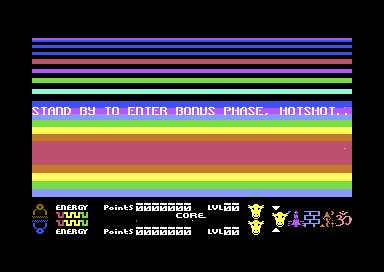
\includegraphics[width=10cm]{src/bonusphase/entry/bonus_entry_example.png}%
\caption{The entry sequence.}
\end{figure}

The entry sequence is an animated cascade of colored bars that appears to roll
down from the top of the screen. You might assume we achieve this effect by simply
drawing a series of colored text-based lines in a tight loop. Not the case:

\begin{figure}[H]
    \centering
    \foreach \l in {0,25,...,890}
    {
      \includegraphics[width=2cm]{src/bonusphase/entry_fill/bonus_entry\l.png}%
    }%
\caption{The entry effect filling the screen.}
\end{figure}

\begin{lstlisting}
EnterBonusPhaseInterruptHandler   
        ...
        LDY backgroundColorIndex
        LDA enterBPRainbowColors,Y
        STA $D021    ;Background Color 0
\end{lstlisting}

What we actually do is update the screen's background color as the raster travels
down the screen. The above three lines do this about 30 times every single paint
of the screen, updating the background color that gets painted as we go. The result
is that each colored bar reflects the background color of the screen at the time
the raster is passing it. The trick is to keep updating the background color at
gradually increasing intervals.

After we update the background color we set the raster interrupt to the next position
we're interested in:

\begin{lstlisting}
EnterBonusPhaseInterruptHandler   
        ...
        LDY backgroundColorIndex
        LDA enterBPRainbowColors,Y
        STA $D021    ;Background Color 0

        ; Check if we've reached the end of the rainbow effect.
        LDA bpRasterPositionArray,Y
        ...
        ; Update the position of the next interrupt.
        CLC 
        ADC $D012    ;Raster Position
        STA $D012    ;Raster Position
\end{lstlisting}

The value we get from \icode{bpRasterPositionArray} reflects our intention of painting
increasingly tall bars:

\begin{lstlisting}
bpRasterPositionArray     .BYTE $01,$01,$01,$01,$02,$02,$02,$02
                          .BYTE $03,$03,$03,$03,$04,$04,$04,$04
                          .BYTE $05,$05,$05,$05,$06,$06,$06,$06
                          .BYTE $07,$07,$07,$07,$07,$07,$00
\end{lstlisting}

Each value in here gets added to the current \index{raster} interrupt position (\icode{ADC \$D012}).
The further we go down the screen the taller the bars become.

\begin{figure}[H]
    \centering
    \foreach \l in {554,...,555}
    {
      \includegraphics[width=6.5cm]{bonusphase/entry/bonus_entry\l.png}%
    }%
  \caption{Updating the background color at a 5 line interval as given by \icode{bpRasterPositionArray}.}
\end{figure}

In addition to drawing incrementally larger bars we're also shifting down by one row the color each one is painted
at each pass. This is responsible for creating the visual effect of each bar moving independently
down the screen.

\begin{figure}[H]
    \centering
    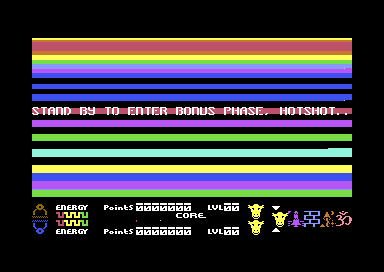
\includegraphics[width=6.5cm]{bonusphase/entry/bonus_entry_from.png}%
    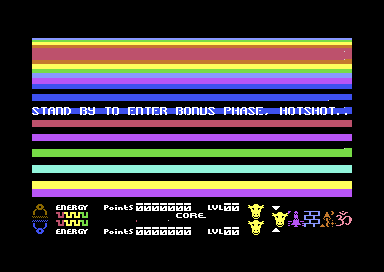
\includegraphics[width=6.5cm]{bonusphase/entry/bonus_entry_to.png}%
  \caption{The color sequences shifts down one position after each full screen paint.}
\end{figure}

This is managed by an array..

\begin{lstlisting}
entryScreenRainbowColors
      .BYTE RED,ORANGE,YELLOW,GREEN,LTBLUE,PURPLE,BLUE,YELLOW
      .BYTE BLACK,CYAN,BLACK,GREEN,BLACK,PURPLE,BLACK,RED
      .BYTE BLACK,BLUE,BLACK,BLUE,BLACK,BLUE,PURPLE,LTBLUE
      .BYTE GREEN,YELLOW,ORANGE,RED
\end{lstlisting}

.. referenced in \icode{UpdateEntryScreenRainbow}. After every full screen paint we update the an
array \icode{previousRoundRainbowColors} to store the position of the previous bar that used it.
This allows us to use \icode{previousRoundRainbowColors} as a source for \icode{X} the next time
we finish a screen and shift the colors along by one position:

\begin{lstlisting}
UpdateEntryScreenRainbow   
        ...
        LDA entryScreenRainbowColors,X
        STA enterBPRainbowColors,Y
        TYA 
        STA previousRoundRainbowColors,X
\end{lstlisting}

All in all, this is a neat effect and would only have been possible at the speeds achieved by using
the raster interrupt in this way. Simply painting the screen with colored text would have been much
slower.

\section{Generating Maps}
\begin{figure}[H]
    \centering
      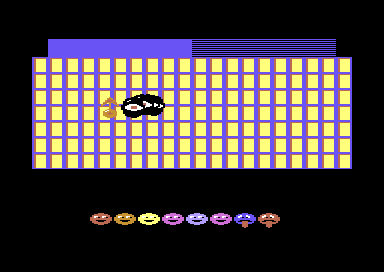
\includegraphics[width=10cm]{src/bonusphase/bonus_phase.png}%
\caption{The beginning of the first bonus phase.}
\end{figure}
Every time the player enters the bonus phase we'll procedurally generate a 
new map. The way we'll manage this is by treating the map a stack of 
256 rows and defining our map simply as an array of the rows that 
make up the map.

  \begin{figure}[H]
      \centering
      \foreach \l in {0,...,6}
      {
        \includegraphics[height=17cm]{src/bonusphase/map\l.png}%
        \hspace{1em}
      }%
  \caption{The first seven maps used by the bonus phase round.}
  \end{figure}

This means that in order to generate a new map all we have to do is come
up with an array of bytes where each byte defines a row in the map. By
way of example, this is what the array that defines the map for the 
first bonus phase round looks like:


\begin{lstlisting}
bonusPhaseMapDefinition 
    .BYTE $00,$00,$00,$00,$00,$00,$00,$00,$00,$00
    .BYTE $11,$11,$11,$11,$11,$11,$11,$11,$11,$11
    .BYTE $11,$11,$11,$11,$11,$11,$11,$11,$11,$11
    .BYTE $15,$16,$16,$16,$16,$16,$16,$16,$16,$17
    .BYTE $15,$16,$16,$16,$16,$16,$16,$16,$16,$17
    .BYTE $13,$13,$13,$13,$13,$13,$13,$13,$13,$13
    .BYTE $15,$16,$16,$16,$16,$16,$16,$16,$16,$17
    .BYTE $14,$14,$00,$15,$16,$17,$00,$00,$14,$14
    .BYTE $00,$14,$14,$14,$14,$14,$14,$14,$14,$00
    .BYTE $00,$00,$00,$00,$00,$00,$00,$00,$00,$00
    .BYTE $00,$14,$14,$14,$14,$14,$14,$14,$14,$00
    .BYTE $14,$14,$00,$15,$16,$17,$00,$00,$14,$14
    .BYTE $15,$16,$16,$16,$16,$16,$16,$16,$16,$17
    .BYTE $00,$14,$14,$14,$14,$14,$14,$14,$14,$00
    .BYTE $00,$15,$16,$17,$00,$00,$15,$16,$17,$00
    .BYTE $13,$13,$13,$13,$13,$13,$13,$13,$13,$13
    .BYTE $15,$16,$16,$16,$16,$16,$16,$16,$16,$17
    .BYTE $11,$11,$11,$11,$11,$11,$11,$11,$11,$11
    .BYTE $00,$00,$00,$00,$00,$00,$00,$00,$00,$00
    .BYTE $12,$12,$12,$12,$12,$12,$12,$12,$12,$00
    .BYTE $00,$15,$16,$17,$00,$00,$15,$16,$17,$00
    .BYTE $00,$15,$16,$17,$00,$00,$15,$16,$17,$00
    .BYTE $13,$13,$13,$13,$13,$13,$13,$13,$13,$13
    .BYTE $12,$12,$12,$12,$12,$12,$12,$12,$12,$00
    .BYTE $11,$11,$11,$11,$11,$11,$11,$11,$11,$11
    .BYTE $10,$10,$10,$10,$10,$10
\end{lstlisting}

This map definition starts from the bottom up, it does this because we
are scrolling upward so it makes sense to begin with what the player
will see first. The start of the map is a simple sequence of zeroes:

\begin{lstlisting}
bonusPhaseMapDefinition 
    .BYTE $00,$00,$00,$00,$00,$00,$00,$00,$00,$00
\end{lstlisting}

This is the row image each line translates to, a regular square pattern
initially followed by rows with some other features.

\begin{figure}[H]
  {
    \setlength{\tabcolsep}{3.0pt}
    \setlength\cmidrulewidth{\heavyrulewidth} % Make cmidrule = 
    \begin{adjustbox}{width=14cm,center}
      \begin{tabular}{cc}
        \toprule
        Index & Image\\
        \midrule
        \icode{\$00} & \makecell[l]{
          
\includegraphics[width=10cm]{src/bonusphase/row_hex00.png}%
        } \\
        \icode{\$00} & \makecell[l]{
          
\includegraphics[width=10cm]{src/bonusphase/row_hex00.png}%
        } \\
        \icode{\$00} & \makecell[l]{
          
\includegraphics[width=10cm]{src/bonusphase/row_hex00.png}%
        } \\
        \icode{\$00} & \makecell[l]{
          
\includegraphics[width=10cm]{src/bonusphase/row_hex00.png}%
        } \\
        \icode{\$00} & \makecell[l]{
          
\includegraphics[width=10cm]{src/bonusphase/row_hex00.png}%
        } \\
        \icode{\$00} & \makecell[l]{
          
\includegraphics[width=10cm]{src/bonusphase/row_hex00.png}%
        } \\
        \icode{\$00} & \makecell[l]{
          
\includegraphics[width=10cm]{src/bonusphase/row_hex00.png}%
        } \\
        \icode{\$00} & \makecell[l]{
          
\includegraphics[width=10cm]{src/bonusphase/row_hex00.png}%
        } \\
        \bottomrule
      \end{tabular}
    \end{adjustbox}
  }\caption{Snapshot of the map created by the first line definition.}
\end{figure}

Further along in the definition we reach a segment where some new features
are introduced.

\begin{lstlisting}
bonusPhaseMapDefinition 
    .BYTE $11,$11,$11,$11,$11,$11,$11,$11,$11,$11
    .BYTE $15,$16,$16,$16,$16,$16,$16,$16,$16,$17
\end{lstlisting}

We can see what each of \icode{\$11,\$15,\$16} translate to when we
map them to their corresponding images:

\begin{figure}[H]
  {
    \setlength{\tabcolsep}{3.0pt}
    \setlength\cmidrulewidth{\heavyrulewidth} % Make cmidrule = 
    \begin{adjustbox}{width=14cm,center}
      \begin{tabular}{cc}
        \toprule
        Index & Image\\
        \midrule
        \icode{\$16} & \makecell[l]{
          
\includegraphics[width=10cm]{src/bonusphase/row_hex16.png}%
        } \\
        \icode{\$16} & \makecell[l]{
          
\includegraphics[width=10cm]{src/bonusphase/row_hex16.png}%
        } \\
        \icode{\$16} & \makecell[l]{
          
\includegraphics[width=10cm]{src/bonusphase/row_hex16.png}%
        } \\
        \icode{\$15} & \makecell[l]{
          
\includegraphics[width=10cm]{src/bonusphase/row_hex15.png}%
        } \\
        \icode{\$11} & \makecell[l]{
          
\includegraphics[width=10cm]{src/bonusphase/row_hex11.png}%
        } \\
        \icode{\$11} & \makecell[l]{
          
\includegraphics[width=10cm]{src/bonusphase/row_hex11.png}%
        } \\
        \icode{\$11} & \makecell[l]{
          
\includegraphics[width=10cm]{src/bonusphase/row_hex11.png}%
        } \\
        \bottomrule
      \end{tabular}
    \end{adjustbox}
  }\caption{Snapshot of the map created by the first line definition.}
\end{figure}

So how do we get from a value like \icode{\$15} to an image that represents
a row on the screen? 

\begin{figure}[H]
  {
    \setlength{\tabcolsep}{3.0pt}
    \setlength\cmidrulewidth{\heavyrulewidth} % Make cmidrule = 
    \begin{adjustbox}{width=14cm,center}
      \begin{tabular}{cc}
        \toprule
        Index & Image\\
        \midrule
        \icode{\$15} & \makecell[l]{
          
\includegraphics[width=10cm]{src/bonusphase/row_hex15.png}%
        }\\
        \bottomrule
      \end{tabular}
    \end{adjustbox}
  }
\end{figure}

We do this by defining each row with yet another array
of bytes. In all we define 32 rows of different types so when we come up
with a map for the level we are simply referencing each of these rows by their
index in the array. Here is the data structure defining each of the 32 rows:

\begin{lstlisting}[basicstyle=\tiny]
bonusPhaseMapRowDefinitions   
        .BYTE $00,$00,$00,$00,$00,$00,$00,$00,$00,$00,$00,$00,$00,$00,$00,$00,$00,$00,$00,$00 ; 00
        .BYTE $0D,$0D,$0E,$0E,$0E,$0E,$0E,$00,$00,$0B,$0B,$00,$00,$0D,$0D,$0D,$0D,$0D,$0E,$0E 
        .BYTE $10,$0B,$0B,$0B,$0B,$0B,$0B,$0B,$0B,$11,$10,$0B,$0B,$0B,$0B,$0B,$0B,$0B,$0B,$11
        .BYTE $0E,$10,$0B,$0B,$0B,$0B,$0B,$0B,$11,$0D,$0E,$10,$0B,$0B,$0B,$0B,$0B,$0B,$11,$0D
        .BYTE $0E,$0E,$10,$0B,$0B,$0B,$0B,$11,$0D,$0D,$0E,$0E,$10,$0B,$0B,$0B,$0B,$11,$0D,$0D
        .BYTE $0E,$0E,$0E,$00,$00,$00,$00,$0D,$0D,$0D,$0E,$0E,$0E,$00,$00,$00,$00,$0D,$0D,$0D
        .BYTE $0E,$0E,$0E,$00,$0A,$0A,$00,$0D,$0D,$0D,$0E,$0E,$0E,$00,$0A,$0A,$00,$0D,$0D,$0D
        .BYTE $0E,$0E,$0E,$00,$09,$09,$00,$0D,$0D,$0D,$0E,$0E,$0E,$00,$09,$09,$00,$0D,$0D,$0D
        .BYTE $0E,$0E,$12,$0C,$0C,$0C,$0C,$13,$0D,$0D,$0E,$0E,$12,$0C,$0C,$0C,$0C,$13,$0D,$0D
        .BYTE $0E,$07,$00,$00,$15,$15,$00,$00,$05,$0D,$0E,$07,$00,$00,$15,$15,$00,$00,$05,$0D
        .BYTE $07,$0F,$00,$00,$15,$15,$00,$00,$0F,$05,$07,$0F,$00,$00,$15,$15,$00,$00,$0F,$05
        .BYTE $17,$17,$00,$00,$18,$17,$00,$00,$18,$18,$17,$17,$00,$00,$18,$17,$00,$00,$18,$18
        .BYTE $0F,$0F,$0F,$00,$00,$00,$00,$0F,$0F,$0F,$0F,$0F,$0F,$00,$00,$00,$00,$0F,$0F,$0F
        .BYTE $00,$00,$09,$09,$00,$00,$09,$09,$00,$00,$00,$00,$09,$09,$00,$00,$09,$09,$00,$00
        .BYTE $00,$00,$0A,$0A,$00,$00,$0A,$0A,$00,$00,$00,$00,$0A,$0A,$00,$00,$0A,$0A,$00,$00
        .BYTE $0F,$0F,$0F,$0F,$0F,$0F,$0F,$0F,$0F,$00,$00,$0F,$0F,$0F,$0F,$0F,$0F,$0F,$0F,$0F ; 0F
        .BYTE $14,$14,$14,$14,$14,$14,$14,$14,$14,$14,$14,$14,$14,$14,$14,$14,$14,$14,$14,$14
        .BYTE $0F,$0E,$0E,$0E,$0E,$0E,$0E,$0E,$0E,$0E,$0D,$0D,$0D,$0D,$0D,$0D,$0D,$0D,$0D,$0F
        .BYTE $0B,$0B,$0B,$00,$0B,$0B,$0B,$0B,$0B,$0F,$0F,$0B,$0B,$0B,$0B,$0B,$00,$0B,$0B,$0B
        .BYTE $15,$15,$15,$15,$15,$15,$15,$15,$15,$15,$15,$15,$15,$15,$15,$15,$15,$15,$15,$15
        .BYTE $00,$00,$00,$0F,$0F,$0F,$00,$00,$00,$0F,$0F,$00,$00,$00,$0F,$0F,$0F,$00,$00,$00
        .BYTE $00,$10,$0B,$11,$00,$00,$10,$0B,$11,$00,$00,$10,$0B,$11,$00,$00,$10,$0B,$11,$00 ; 15 
        .BYTE $00,$0E,$00,$0D,$00,$00,$0E,$00,$0D,$00,$00,$0E,$00,$0D,$00,$00,$0E,$00,$0D,$00
        .BYTE $00,$12,$0C,$13,$00,$00,$12,$0C,$13,$00,$00,$12,$0C,$13,$00,$00,$12,$0C,$13,$00
        .BYTE $0F,$0E,$00,$00,$00,$00,$0D,$0F,$0F,$0F,$0F,$0F,$0F,$0E,$0B,$0B,$0B,$0B,$0D,$0F
        .BYTE $0F,$0E,$0B,$0B,$0B,$0B,$0D,$0F,$0F,$0F,$0F,$0F,$0F,$0E,$00,$00,$00,$00,$0D,$0F
        .BYTE $0F,$0E,$00,$00,$00,$00,$0D,$0F,$0F,$0F,$0F,$0F,$0F,$0E,$00,$00,$00,$00,$0D,$0F
        .BYTE $15,$15,$00,$00,$16,$16,$00,$00,$15,$15,$00,$00,$16,$16,$00,$00,$15,$15,$00,$00
        .BYTE $00,$00,$16,$16,$00,$00,$15,$15,$00,$00,$16,$16,$00,$00,$15,$15,$00,$00,$16,$16
        .BYTE $0B,$0B,$0B,$0B,$0B,$0B,$0B,$0B,$0B,$0B,$0B,$0B,$0B,$0B,$0B,$0B,$0B,$0B,$0B,$0B
        .BYTE $0C,$0C,$0C,$0C,$0C,$0C,$0C,$0C,$0C,$0C,$0C,$0C,$0C,$0C,$0C,$0C,$0C,$0C,$0C,$0C
        .BYTE $09,$09,$09,$09,$09,$09,$09,$09,$09,$15,$15,$09,$09,$09,$09,$09,$09,$09,$09,$09
        .BYTE $0A,$0A,$0A,$0A,$0A,$0A,$0A,$0A,$0A,$15,$15,$0A,$0A,$0A,$0A,$0A,$0A,$0A,$0A,$0A
\end{lstlisting}

The one at index \icode{\$15} (21 in decimal) is this guy:

\begin{lstlisting}[basicstyle=\tiny]
bonusPhaseMapRowDefinitions   
        .BYTE $00,$10,$0B,$11,$00,$00,$10,$0B,$11,$00,$00,$10,$0B,$11,$00,$00,$10,$0B,$11,$00
\end{lstlisting}

Each byte in this definition represents a square cell of four bytes. So for example, \icode{\$00}
translates to:

\begin{figure}[H]
  {
    \begin{adjustbox}{width=2cm,center}
        
\includegraphics[width=2cm]{src/bonusphase/row21_cell0.png}%
    \end{adjustbox}
  }
\end{figure}

\captionsetup[subfigure]{font=large,labelfont=large,labelformat=empty}
And the first five bytes (which are repeated four times to complete the full row) translate as follows:
\begin{figure}[H]
  {
    \setlength{\tabcolsep}{3.0pt}
    \setlength\cmidrulewidth{\heavyrulewidth} % Make cmidrule = 
    \begin{adjustbox}{width=15cm,center}
      \begin{subfigure}{0.3\textwidth}
        
\includegraphics[width=3cm]{src/bonusphase/row21_cell0.png}%
        \caption{\icode{\$00}}
      \end{subfigure}
      \begin{subfigure}{0.3\textwidth}
        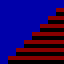
\includegraphics[width=3cm]{src/bonusphase/row21_cell1.png}%
        \caption{\icode{\$10}}
      \end{subfigure}
      \begin{subfigure}{0.3\textwidth}
        
\includegraphics[width=3cm]{src/bonusphase/row21_cell2.png}%
        \caption{\icode{\$0B}}
      \end{subfigure}
      \begin{subfigure}{0.3\textwidth}
        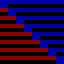
\includegraphics[width=3cm]{src/bonusphase/row21_cell3.png}%
        \caption{\icode{\$11}}
      \end{subfigure}
      \begin{subfigure}{0.3\textwidth}
        
\includegraphics[width=3cm]{src/bonusphase/row21_cell4.png}%
        \caption{\icode{\$00}}
      \end{subfigure}
    \end{adjustbox}
  }
\end{figure}
\captionsetup[subfigure]{font=footnotesize,labelfont=footnotesize,labelformat=empty}

So how do we go from a single byte like \icode{\$00} to a four-byte square? Would you be surprised
if I told you it involved another array of bytes? In fact it involves two arrays of bytes.

\begin{lstlisting}
cellFirstColumnArray
        .BYTE $40,$41,$44,$47,$48,$49,$4F,$4D
        .BYTE $50,$51,$54,$56,$5B,$59,$5C,$5D
        .BYTE $60,$61,$64,$65,$68,$69,$47,$47
        .BYTE $4E,$4E,$57,$57,$5D,$5D,$20,$20
        .BYTE $5D,$45,$4B,$47,$4C,$5D,$4E,$52
        .BYTE $7C,$7D,$6C,$6D,$70,$71,$74,$75
        .BYTE $78,$79
cellSecondColumnArray   
        .BYTE $42,$43,$46,$47,$4A,$48,$4E,$4F
        .BYTE $51,$53,$56,$57,$5A,$5B,$5E,$5C
        .BYTE $61,$63,$66,$67,$6A,$6B,$47,$47
        .BYTE $4E,$4E,$57,$57,$5D,$5D,$20,$20
        .BYTE $45,$47,$57,$4B,$4E,$4C,$52,$57
        .BYTE $7E,$7F,$6E,$6F,$72,$73,$76,$77
        .BYTE $7A,$7B
\end{lstlisting}


So let's look at how we from \icode{\$00} to ...

\begin{figure}[H]
  {
    \begin{adjustbox}{width=2cm,center}
        
\includegraphics[width=2cm]{src/bonusphase/row21_cell0.png}%
    \end{adjustbox}
  }
\end{figure}

.. using the two arrays above. The value \icode{\$00} is treated as in index into each array, so it
points us to the first byte in each. However we're not interested in just the first value in each array
but the first two. So the bytes that we will use to construct the 4-byte square are:


\begin{lstlisting}
cellFirstColumnArray
        .BYTE $40,$41
cellSecondColumnArray   
        .BYTE $42,$43
\end{lstlisting}

Each of these bytes is a reference to a byte in the bonus phase character set. When we set out the
characters in a table as they are eventually laid out we begin to get a sense of what we must do
to turn them into our 4-byte cell:

\begin{figure}[H]                          
{                                          
  \setlength{\tabcolsep}{3.0pt}            
  \setlength\cmidrulewidth{\lightrulewidth}
    \begin{adjustbox}{width=5cm,center}
\begin{subfigure}{0.12\textwidth}

    \begin{figure}[H]
      {
        \setlength{\tabcolsep}{3.0pt}
        \setlength\cmidrulewidth{\lightrulewidth} % Make cmidrule = 
        \begin{adjustbox}{width=0.5cm,center}
          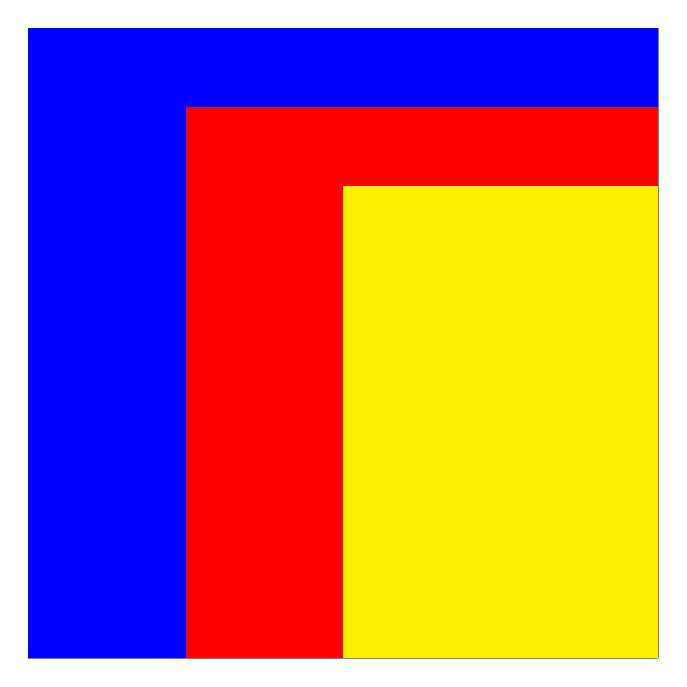
\begin{tikzpicture}
    
\def\BACKGROUNDONE{yellow}
\def\BACKGROUNDTWO{blue}
\def\CHARCOLOR{red}
	\draw[step=1.0,gray,thin] (0,0) grid (8,8);
	\fill[\BACKGROUNDTWO] (0,7) rectangle ++ (1,1);
	\fill[\BACKGROUNDTWO] (1,7) rectangle ++ (1,1);
	\fill[\BACKGROUNDTWO] (2,7) rectangle ++ (1,1);
	\fill[\BACKGROUNDTWO] (3,7) rectangle ++ (1,1);
	\fill[\BACKGROUNDTWO] (4,7) rectangle ++ (1,1);
	\fill[\BACKGROUNDTWO] (5,7) rectangle ++ (1,1);
	\fill[\BACKGROUNDTWO] (6,7) rectangle ++ (1,1);
	\fill[\BACKGROUNDTWO] (7,7) rectangle ++ (1,1);
	\fill[\BACKGROUNDTWO] (0,6) rectangle ++ (1,1);
	\fill[\BACKGROUNDTWO] (1,6) rectangle ++ (1,1);
	\fill[\CHARCOLOR] (2,6) rectangle ++ (1,1);
	\fill[\CHARCOLOR] (3,6) rectangle ++ (1,1);
	\fill[\CHARCOLOR] (4,6) rectangle ++ (1,1);
	\fill[\CHARCOLOR] (5,6) rectangle ++ (1,1);
	\fill[\CHARCOLOR] (6,6) rectangle ++ (1,1);
	\fill[\CHARCOLOR] (7,6) rectangle ++ (1,1);
	\fill[\BACKGROUNDTWO] (0,5) rectangle ++ (1,1);
	\fill[\BACKGROUNDTWO] (1,5) rectangle ++ (1,1);
	\fill[\CHARCOLOR] (2,5) rectangle ++ (1,1);
	\fill[\CHARCOLOR] (3,5) rectangle ++ (1,1);
	\fill[\BACKGROUNDONE] (4,5) rectangle ++ (1,1);
	\fill[\BACKGROUNDONE] (5,5) rectangle ++ (1,1);
	\fill[\BACKGROUNDONE] (6,5) rectangle ++ (1,1);
	\fill[\BACKGROUNDONE] (7,5) rectangle ++ (1,1);
	\fill[\BACKGROUNDTWO] (0,4) rectangle ++ (1,1);
	\fill[\BACKGROUNDTWO] (1,4) rectangle ++ (1,1);
	\fill[\CHARCOLOR] (2,4) rectangle ++ (1,1);
	\fill[\CHARCOLOR] (3,4) rectangle ++ (1,1);
	\fill[\BACKGROUNDONE] (4,4) rectangle ++ (1,1);
	\fill[\BACKGROUNDONE] (5,4) rectangle ++ (1,1);
	\fill[\BACKGROUNDONE] (6,4) rectangle ++ (1,1);
	\fill[\BACKGROUNDONE] (7,4) rectangle ++ (1,1);
	\fill[\BACKGROUNDTWO] (0,3) rectangle ++ (1,1);
	\fill[\BACKGROUNDTWO] (1,3) rectangle ++ (1,1);
	\fill[\CHARCOLOR] (2,3) rectangle ++ (1,1);
	\fill[\CHARCOLOR] (3,3) rectangle ++ (1,1);
	\fill[\BACKGROUNDONE] (4,3) rectangle ++ (1,1);
	\fill[\BACKGROUNDONE] (5,3) rectangle ++ (1,1);
	\fill[\BACKGROUNDONE] (6,3) rectangle ++ (1,1);
	\fill[\BACKGROUNDONE] (7,3) rectangle ++ (1,1);
	\fill[\BACKGROUNDTWO] (0,2) rectangle ++ (1,1);
	\fill[\BACKGROUNDTWO] (1,2) rectangle ++ (1,1);
	\fill[\CHARCOLOR] (2,2) rectangle ++ (1,1);
	\fill[\CHARCOLOR] (3,2) rectangle ++ (1,1);
	\fill[\BACKGROUNDONE] (4,2) rectangle ++ (1,1);
	\fill[\BACKGROUNDONE] (5,2) rectangle ++ (1,1);
	\fill[\BACKGROUNDONE] (6,2) rectangle ++ (1,1);
	\fill[\BACKGROUNDONE] (7,2) rectangle ++ (1,1);
	\fill[\BACKGROUNDTWO] (0,1) rectangle ++ (1,1);
	\fill[\BACKGROUNDTWO] (1,1) rectangle ++ (1,1);
	\fill[\CHARCOLOR] (2,1) rectangle ++ (1,1);
	\fill[\CHARCOLOR] (3,1) rectangle ++ (1,1);
	\fill[\BACKGROUNDONE] (4,1) rectangle ++ (1,1);
	\fill[\BACKGROUNDONE] (5,1) rectangle ++ (1,1);
	\fill[\BACKGROUNDONE] (6,1) rectangle ++ (1,1);
	\fill[\BACKGROUNDONE] (7,1) rectangle ++ (1,1);
	\fill[\BACKGROUNDTWO] (0,0) rectangle ++ (1,1);
	\fill[\BACKGROUNDTWO] (1,0) rectangle ++ (1,1);
	\fill[\CHARCOLOR] (2,0) rectangle ++ (1,1);
	\fill[\CHARCOLOR] (3,0) rectangle ++ (1,1);
	\fill[\BACKGROUNDONE] (4,0) rectangle ++ (1,1);
	\fill[\BACKGROUNDONE] (5,0) rectangle ++ (1,1);
	\fill[\BACKGROUNDONE] (6,0) rectangle ++ (1,1);
	\fill[\BACKGROUNDONE] (7,0) rectangle ++ (1,1);

          \end{tikzpicture}
        \end{adjustbox}
      }\caption*{\$40}
    \end{figure}
    
\end{subfigure}
\begin{subfigure}{0.12\textwidth}

    \begin{figure}[H]
      {
        \setlength{\tabcolsep}{3.0pt}
        \setlength\cmidrulewidth{\lightrulewidth} % Make cmidrule = 
        \begin{adjustbox}{width=0.5cm,center}
          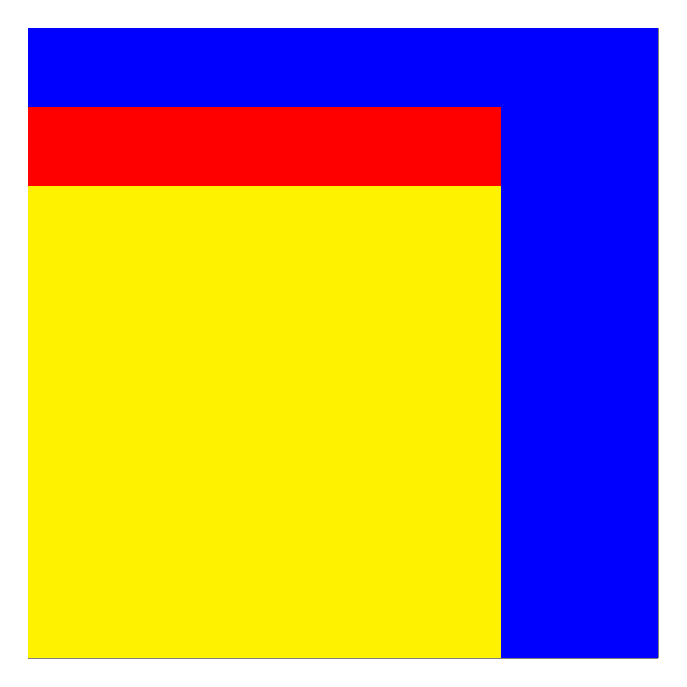
\begin{tikzpicture}
    
\def\BACKGROUNDONE{yellow}
\def\BACKGROUNDTWO{blue}
\def\CHARCOLOR{red}
	\draw[step=1.0,gray,thin] (0,0) grid (8,8);
	\fill[\BACKGROUNDTWO] (0,7) rectangle ++ (1,1);
	\fill[\BACKGROUNDTWO] (1,7) rectangle ++ (1,1);
	\fill[\BACKGROUNDTWO] (2,7) rectangle ++ (1,1);
	\fill[\BACKGROUNDTWO] (3,7) rectangle ++ (1,1);
	\fill[\BACKGROUNDTWO] (4,7) rectangle ++ (1,1);
	\fill[\BACKGROUNDTWO] (5,7) rectangle ++ (1,1);
	\fill[\BACKGROUNDTWO] (6,7) rectangle ++ (1,1);
	\fill[\BACKGROUNDTWO] (7,7) rectangle ++ (1,1);
	\fill[\CHARCOLOR] (0,6) rectangle ++ (1,1);
	\fill[\CHARCOLOR] (1,6) rectangle ++ (1,1);
	\fill[\CHARCOLOR] (2,6) rectangle ++ (1,1);
	\fill[\CHARCOLOR] (3,6) rectangle ++ (1,1);
	\fill[\CHARCOLOR] (4,6) rectangle ++ (1,1);
	\fill[\CHARCOLOR] (5,6) rectangle ++ (1,1);
	\fill[\BACKGROUNDTWO] (6,6) rectangle ++ (1,1);
	\fill[\BACKGROUNDTWO] (7,6) rectangle ++ (1,1);
	\fill[\BACKGROUNDONE] (0,5) rectangle ++ (1,1);
	\fill[\BACKGROUNDONE] (1,5) rectangle ++ (1,1);
	\fill[\BACKGROUNDONE] (2,5) rectangle ++ (1,1);
	\fill[\BACKGROUNDONE] (3,5) rectangle ++ (1,1);
	\fill[\BACKGROUNDONE] (4,5) rectangle ++ (1,1);
	\fill[\BACKGROUNDONE] (5,5) rectangle ++ (1,1);
	\fill[\BACKGROUNDTWO] (6,5) rectangle ++ (1,1);
	\fill[\BACKGROUNDTWO] (7,5) rectangle ++ (1,1);
	\fill[\BACKGROUNDONE] (0,4) rectangle ++ (1,1);
	\fill[\BACKGROUNDONE] (1,4) rectangle ++ (1,1);
	\fill[\BACKGROUNDONE] (2,4) rectangle ++ (1,1);
	\fill[\BACKGROUNDONE] (3,4) rectangle ++ (1,1);
	\fill[\BACKGROUNDONE] (4,4) rectangle ++ (1,1);
	\fill[\BACKGROUNDONE] (5,4) rectangle ++ (1,1);
	\fill[\BACKGROUNDTWO] (6,4) rectangle ++ (1,1);
	\fill[\BACKGROUNDTWO] (7,4) rectangle ++ (1,1);
	\fill[\BACKGROUNDONE] (0,3) rectangle ++ (1,1);
	\fill[\BACKGROUNDONE] (1,3) rectangle ++ (1,1);
	\fill[\BACKGROUNDONE] (2,3) rectangle ++ (1,1);
	\fill[\BACKGROUNDONE] (3,3) rectangle ++ (1,1);
	\fill[\BACKGROUNDONE] (4,3) rectangle ++ (1,1);
	\fill[\BACKGROUNDONE] (5,3) rectangle ++ (1,1);
	\fill[\BACKGROUNDTWO] (6,3) rectangle ++ (1,1);
	\fill[\BACKGROUNDTWO] (7,3) rectangle ++ (1,1);
	\fill[\BACKGROUNDONE] (0,2) rectangle ++ (1,1);
	\fill[\BACKGROUNDONE] (1,2) rectangle ++ (1,1);
	\fill[\BACKGROUNDONE] (2,2) rectangle ++ (1,1);
	\fill[\BACKGROUNDONE] (3,2) rectangle ++ (1,1);
	\fill[\BACKGROUNDONE] (4,2) rectangle ++ (1,1);
	\fill[\BACKGROUNDONE] (5,2) rectangle ++ (1,1);
	\fill[\BACKGROUNDTWO] (6,2) rectangle ++ (1,1);
	\fill[\BACKGROUNDTWO] (7,2) rectangle ++ (1,1);
	\fill[\BACKGROUNDONE] (0,1) rectangle ++ (1,1);
	\fill[\BACKGROUNDONE] (1,1) rectangle ++ (1,1);
	\fill[\BACKGROUNDONE] (2,1) rectangle ++ (1,1);
	\fill[\BACKGROUNDONE] (3,1) rectangle ++ (1,1);
	\fill[\BACKGROUNDONE] (4,1) rectangle ++ (1,1);
	\fill[\BACKGROUNDONE] (5,1) rectangle ++ (1,1);
	\fill[\BACKGROUNDTWO] (6,1) rectangle ++ (1,1);
	\fill[\BACKGROUNDTWO] (7,1) rectangle ++ (1,1);
	\fill[\BACKGROUNDONE] (0,0) rectangle ++ (1,1);
	\fill[\BACKGROUNDONE] (1,0) rectangle ++ (1,1);
	\fill[\BACKGROUNDONE] (2,0) rectangle ++ (1,1);
	\fill[\BACKGROUNDONE] (3,0) rectangle ++ (1,1);
	\fill[\BACKGROUNDONE] (4,0) rectangle ++ (1,1);
	\fill[\BACKGROUNDONE] (5,0) rectangle ++ (1,1);
	\fill[\BACKGROUNDTWO] (6,0) rectangle ++ (1,1);
	\fill[\BACKGROUNDTWO] (7,0) rectangle ++ (1,1);

          \end{tikzpicture}
        \end{adjustbox}
      }\caption*{\$42}
    \end{figure}
    
\end{subfigure}
    \end{adjustbox}
    \begin{adjustbox}{width=5cm,center}
\begin{subfigure}{0.12\textwidth}

    \begin{figure}[H]
      {
        \setlength{\tabcolsep}{3.0pt}
        \setlength\cmidrulewidth{\lightrulewidth} % Make cmidrule = 
        \begin{adjustbox}{width=0.5cm,center}
          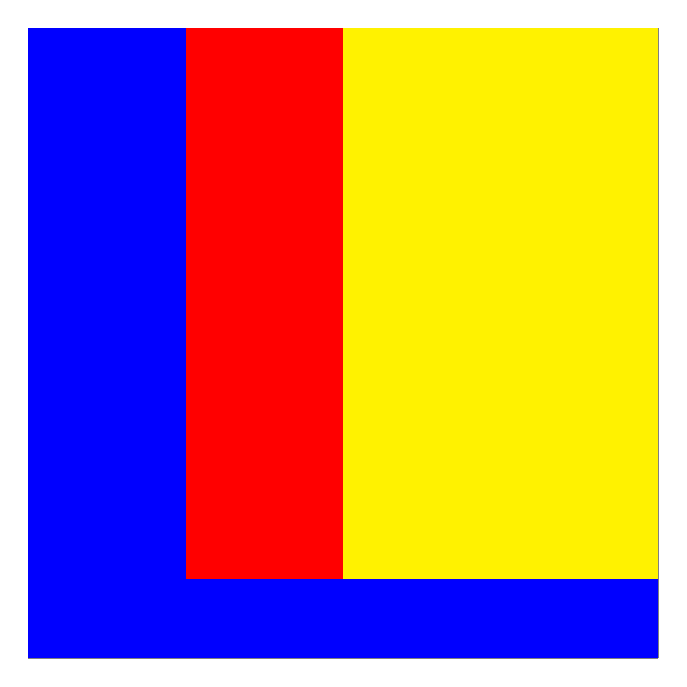
\begin{tikzpicture}
    
\def\BACKGROUNDONE{yellow}
\def\BACKGROUNDTWO{blue}
\def\CHARCOLOR{red}
	\draw[step=1.0,gray,thin] (0,0) grid (8,8);
	\fill[\BACKGROUNDTWO] (0,7) rectangle ++ (1,1);
	\fill[\BACKGROUNDTWO] (1,7) rectangle ++ (1,1);
	\fill[\CHARCOLOR] (2,7) rectangle ++ (1,1);
	\fill[\CHARCOLOR] (3,7) rectangle ++ (1,1);
	\fill[\BACKGROUNDONE] (4,7) rectangle ++ (1,1);
	\fill[\BACKGROUNDONE] (5,7) rectangle ++ (1,1);
	\fill[\BACKGROUNDONE] (6,7) rectangle ++ (1,1);
	\fill[\BACKGROUNDONE] (7,7) rectangle ++ (1,1);
	\fill[\BACKGROUNDTWO] (0,6) rectangle ++ (1,1);
	\fill[\BACKGROUNDTWO] (1,6) rectangle ++ (1,1);
	\fill[\CHARCOLOR] (2,6) rectangle ++ (1,1);
	\fill[\CHARCOLOR] (3,6) rectangle ++ (1,1);
	\fill[\BACKGROUNDONE] (4,6) rectangle ++ (1,1);
	\fill[\BACKGROUNDONE] (5,6) rectangle ++ (1,1);
	\fill[\BACKGROUNDONE] (6,6) rectangle ++ (1,1);
	\fill[\BACKGROUNDONE] (7,6) rectangle ++ (1,1);
	\fill[\BACKGROUNDTWO] (0,5) rectangle ++ (1,1);
	\fill[\BACKGROUNDTWO] (1,5) rectangle ++ (1,1);
	\fill[\CHARCOLOR] (2,5) rectangle ++ (1,1);
	\fill[\CHARCOLOR] (3,5) rectangle ++ (1,1);
	\fill[\BACKGROUNDONE] (4,5) rectangle ++ (1,1);
	\fill[\BACKGROUNDONE] (5,5) rectangle ++ (1,1);
	\fill[\BACKGROUNDONE] (6,5) rectangle ++ (1,1);
	\fill[\BACKGROUNDONE] (7,5) rectangle ++ (1,1);
	\fill[\BACKGROUNDTWO] (0,4) rectangle ++ (1,1);
	\fill[\BACKGROUNDTWO] (1,4) rectangle ++ (1,1);
	\fill[\CHARCOLOR] (2,4) rectangle ++ (1,1);
	\fill[\CHARCOLOR] (3,4) rectangle ++ (1,1);
	\fill[\BACKGROUNDONE] (4,4) rectangle ++ (1,1);
	\fill[\BACKGROUNDONE] (5,4) rectangle ++ (1,1);
	\fill[\BACKGROUNDONE] (6,4) rectangle ++ (1,1);
	\fill[\BACKGROUNDONE] (7,4) rectangle ++ (1,1);
	\fill[\BACKGROUNDTWO] (0,3) rectangle ++ (1,1);
	\fill[\BACKGROUNDTWO] (1,3) rectangle ++ (1,1);
	\fill[\CHARCOLOR] (2,3) rectangle ++ (1,1);
	\fill[\CHARCOLOR] (3,3) rectangle ++ (1,1);
	\fill[\BACKGROUNDONE] (4,3) rectangle ++ (1,1);
	\fill[\BACKGROUNDONE] (5,3) rectangle ++ (1,1);
	\fill[\BACKGROUNDONE] (6,3) rectangle ++ (1,1);
	\fill[\BACKGROUNDONE] (7,3) rectangle ++ (1,1);
	\fill[\BACKGROUNDTWO] (0,2) rectangle ++ (1,1);
	\fill[\BACKGROUNDTWO] (1,2) rectangle ++ (1,1);
	\fill[\CHARCOLOR] (2,2) rectangle ++ (1,1);
	\fill[\CHARCOLOR] (3,2) rectangle ++ (1,1);
	\fill[\BACKGROUNDONE] (4,2) rectangle ++ (1,1);
	\fill[\BACKGROUNDONE] (5,2) rectangle ++ (1,1);
	\fill[\BACKGROUNDONE] (6,2) rectangle ++ (1,1);
	\fill[\BACKGROUNDONE] (7,2) rectangle ++ (1,1);
	\fill[\BACKGROUNDTWO] (0,1) rectangle ++ (1,1);
	\fill[\BACKGROUNDTWO] (1,1) rectangle ++ (1,1);
	\fill[\CHARCOLOR] (2,1) rectangle ++ (1,1);
	\fill[\CHARCOLOR] (3,1) rectangle ++ (1,1);
	\fill[\BACKGROUNDONE] (4,1) rectangle ++ (1,1);
	\fill[\BACKGROUNDONE] (5,1) rectangle ++ (1,1);
	\fill[\BACKGROUNDONE] (6,1) rectangle ++ (1,1);
	\fill[\BACKGROUNDONE] (7,1) rectangle ++ (1,1);
	\fill[\BACKGROUNDTWO] (0,0) rectangle ++ (1,1);
	\fill[\BACKGROUNDTWO] (1,0) rectangle ++ (1,1);
	\fill[\BACKGROUNDTWO] (2,0) rectangle ++ (1,1);
	\fill[\BACKGROUNDTWO] (3,0) rectangle ++ (1,1);
	\fill[\BACKGROUNDTWO] (4,0) rectangle ++ (1,1);
	\fill[\BACKGROUNDTWO] (5,0) rectangle ++ (1,1);
	\fill[\BACKGROUNDTWO] (6,0) rectangle ++ (1,1);
	\fill[\BACKGROUNDTWO] (7,0) rectangle ++ (1,1);

          \end{tikzpicture}
        \end{adjustbox}
      }\caption*{\$41}
    \end{figure}
    
\end{subfigure}
\begin{subfigure}{0.12\textwidth}

    \begin{figure}[H]
      {
        \setlength{\tabcolsep}{3.0pt}
        \setlength\cmidrulewidth{\lightrulewidth} % Make cmidrule = 
        \begin{adjustbox}{width=0.5cm,center}
          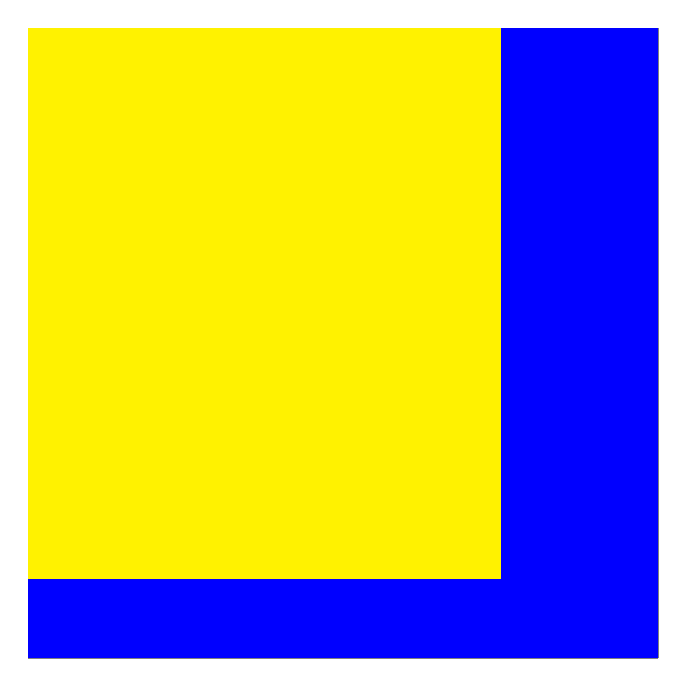
\begin{tikzpicture}
    
\def\BACKGROUNDONE{yellow}
\def\BACKGROUNDTWO{blue}
\def\CHARCOLOR{red}
	\draw[step=1.0,gray,thin] (0,0) grid (8,8);
	\fill[\BACKGROUNDONE] (0,7) rectangle ++ (1,1);
	\fill[\BACKGROUNDONE] (1,7) rectangle ++ (1,1);
	\fill[\BACKGROUNDONE] (2,7) rectangle ++ (1,1);
	\fill[\BACKGROUNDONE] (3,7) rectangle ++ (1,1);
	\fill[\BACKGROUNDONE] (4,7) rectangle ++ (1,1);
	\fill[\BACKGROUNDONE] (5,7) rectangle ++ (1,1);
	\fill[\BACKGROUNDTWO] (6,7) rectangle ++ (1,1);
	\fill[\BACKGROUNDTWO] (7,7) rectangle ++ (1,1);
	\fill[\BACKGROUNDONE] (0,6) rectangle ++ (1,1);
	\fill[\BACKGROUNDONE] (1,6) rectangle ++ (1,1);
	\fill[\BACKGROUNDONE] (2,6) rectangle ++ (1,1);
	\fill[\BACKGROUNDONE] (3,6) rectangle ++ (1,1);
	\fill[\BACKGROUNDONE] (4,6) rectangle ++ (1,1);
	\fill[\BACKGROUNDONE] (5,6) rectangle ++ (1,1);
	\fill[\BACKGROUNDTWO] (6,6) rectangle ++ (1,1);
	\fill[\BACKGROUNDTWO] (7,6) rectangle ++ (1,1);
	\fill[\BACKGROUNDONE] (0,5) rectangle ++ (1,1);
	\fill[\BACKGROUNDONE] (1,5) rectangle ++ (1,1);
	\fill[\BACKGROUNDONE] (2,5) rectangle ++ (1,1);
	\fill[\BACKGROUNDONE] (3,5) rectangle ++ (1,1);
	\fill[\BACKGROUNDONE] (4,5) rectangle ++ (1,1);
	\fill[\BACKGROUNDONE] (5,5) rectangle ++ (1,1);
	\fill[\BACKGROUNDTWO] (6,5) rectangle ++ (1,1);
	\fill[\BACKGROUNDTWO] (7,5) rectangle ++ (1,1);
	\fill[\BACKGROUNDONE] (0,4) rectangle ++ (1,1);
	\fill[\BACKGROUNDONE] (1,4) rectangle ++ (1,1);
	\fill[\BACKGROUNDONE] (2,4) rectangle ++ (1,1);
	\fill[\BACKGROUNDONE] (3,4) rectangle ++ (1,1);
	\fill[\BACKGROUNDONE] (4,4) rectangle ++ (1,1);
	\fill[\BACKGROUNDONE] (5,4) rectangle ++ (1,1);
	\fill[\BACKGROUNDTWO] (6,4) rectangle ++ (1,1);
	\fill[\BACKGROUNDTWO] (7,4) rectangle ++ (1,1);
	\fill[\BACKGROUNDONE] (0,3) rectangle ++ (1,1);
	\fill[\BACKGROUNDONE] (1,3) rectangle ++ (1,1);
	\fill[\BACKGROUNDONE] (2,3) rectangle ++ (1,1);
	\fill[\BACKGROUNDONE] (3,3) rectangle ++ (1,1);
	\fill[\BACKGROUNDONE] (4,3) rectangle ++ (1,1);
	\fill[\BACKGROUNDONE] (5,3) rectangle ++ (1,1);
	\fill[\BACKGROUNDTWO] (6,3) rectangle ++ (1,1);
	\fill[\BACKGROUNDTWO] (7,3) rectangle ++ (1,1);
	\fill[\BACKGROUNDONE] (0,2) rectangle ++ (1,1);
	\fill[\BACKGROUNDONE] (1,2) rectangle ++ (1,1);
	\fill[\BACKGROUNDONE] (2,2) rectangle ++ (1,1);
	\fill[\BACKGROUNDONE] (3,2) rectangle ++ (1,1);
	\fill[\BACKGROUNDONE] (4,2) rectangle ++ (1,1);
	\fill[\BACKGROUNDONE] (5,2) rectangle ++ (1,1);
	\fill[\BACKGROUNDTWO] (6,2) rectangle ++ (1,1);
	\fill[\BACKGROUNDTWO] (7,2) rectangle ++ (1,1);
	\fill[\BACKGROUNDONE] (0,1) rectangle ++ (1,1);
	\fill[\BACKGROUNDONE] (1,1) rectangle ++ (1,1);
	\fill[\BACKGROUNDONE] (2,1) rectangle ++ (1,1);
	\fill[\BACKGROUNDONE] (3,1) rectangle ++ (1,1);
	\fill[\BACKGROUNDONE] (4,1) rectangle ++ (1,1);
	\fill[\BACKGROUNDONE] (5,1) rectangle ++ (1,1);
	\fill[\BACKGROUNDTWO] (6,1) rectangle ++ (1,1);
	\fill[\BACKGROUNDTWO] (7,1) rectangle ++ (1,1);
	\fill[\BACKGROUNDTWO] (0,0) rectangle ++ (1,1);
	\fill[\BACKGROUNDTWO] (1,0) rectangle ++ (1,1);
	\fill[\BACKGROUNDTWO] (2,0) rectangle ++ (1,1);
	\fill[\BACKGROUNDTWO] (3,0) rectangle ++ (1,1);
	\fill[\BACKGROUNDTWO] (4,0) rectangle ++ (1,1);
	\fill[\BACKGROUNDTWO] (5,0) rectangle ++ (1,1);
	\fill[\BACKGROUNDTWO] (6,0) rectangle ++ (1,1);
	\fill[\BACKGROUNDTWO] (7,0) rectangle ++ (1,1);

          \end{tikzpicture}
        \end{adjustbox}
      }\caption*{\$43}
    \end{figure}
    
\end{subfigure}
    \end{adjustbox}
  }\caption[]{Characters making up the four-byte cell referenced by \icode{\$00}.}
\end{figure}

What we have done is take the two values at index \icode{\$00} in \icode{cellFirstColumnArray}
and used each as the first column across two rows. Then we've taken the two values from
\icode{cellSecondColumnArray} and used them as the second column across two rows. 

Let's repeat this process for the values given by index \icode{\$10} highlighted in red. 

\begin{lstlisting}
cellFirstColumnArray
        .BYTE $40,$41,$44,$47,$48,$49,$4F,$4D
        .BYTE $50,$51,$54,$56,$5B,$59,$5C,$5D
        .BYTE $60,$61,$64,$65,$68,$69,$47,$47
        ...
cellSecondColumnArray   
        .BYTE $42,$43,$46,$47,$4A,$48,$4E,$4F
        .BYTE $51,$53,$56,$57,$5A,$5B,$5E,$5C
        .BYTE $61,$63,$66,$67,$6A,$6B,$47,$47
        ...
\end{lstlisting}

The values at index \icode{\$10} in \icode{cellFirstColumnArray} are \icode{\$60,\$61} and
in \icode{cellSecondColumnArray} are \icode{\$61,\$63}. Translated to row and column position
this gives:

\begin{figure}[H]                          
{                                          
  \setlength{\tabcolsep}{3.0pt}            
  \setlength\cmidrulewidth{\lightrulewidth}
    \begin{adjustbox}{width=5cm,center}
\begin{subfigure}{0.12\textwidth}

    \begin{figure}[H]
      {
        \setlength{\tabcolsep}{3.0pt}
        \setlength\cmidrulewidth{\lightrulewidth} % Make cmidrule = 
        \begin{adjustbox}{width=0.5cm,center}
          
\begin{tikzpicture}
    
\def\BACKGROUNDONE{yellow}
\def\BACKGROUNDTWO{blue}
\def\CHARCOLOR{red}
	\draw[step=1.0,gray,thin] (0,0) grid (8,8);
	\fill[\BACKGROUNDTWO] (0,7) rectangle ++ (1,1);
	\fill[\BACKGROUNDTWO] (1,7) rectangle ++ (1,1);
	\fill[\BACKGROUNDTWO] (2,7) rectangle ++ (1,1);
	\fill[\BACKGROUNDTWO] (3,7) rectangle ++ (1,1);
	\fill[\BACKGROUNDTWO] (4,7) rectangle ++ (1,1);
	\fill[\BACKGROUNDTWO] (5,7) rectangle ++ (1,1);
	\fill[\BACKGROUNDTWO] (6,7) rectangle ++ (1,1);
	\fill[\BACKGROUNDTWO] (7,7) rectangle ++ (1,1);
	\fill[\BACKGROUNDTWO] (0,6) rectangle ++ (1,1);
	\fill[\BACKGROUNDTWO] (1,6) rectangle ++ (1,1);
	\fill[\BACKGROUNDTWO] (2,6) rectangle ++ (1,1);
	\fill[\BACKGROUNDTWO] (3,6) rectangle ++ (1,1);
	\fill[\BACKGROUNDTWO] (4,6) rectangle ++ (1,1);
	\fill[\BACKGROUNDTWO] (5,6) rectangle ++ (1,1);
	\fill[\BACKGROUNDTWO] (6,6) rectangle ++ (1,1);
	\fill[\BACKGROUNDTWO] (7,6) rectangle ++ (1,1);
	\fill[\BACKGROUNDTWO] (0,5) rectangle ++ (1,1);
	\fill[\BACKGROUNDTWO] (1,5) rectangle ++ (1,1);
	\fill[\BACKGROUNDTWO] (2,5) rectangle ++ (1,1);
	\fill[\BACKGROUNDTWO] (3,5) rectangle ++ (1,1);
	\fill[\BACKGROUNDTWO] (4,5) rectangle ++ (1,1);
	\fill[\BACKGROUNDTWO] (5,5) rectangle ++ (1,1);
	\fill[\BACKGROUNDTWO] (6,5) rectangle ++ (1,1);
	\fill[\BACKGROUNDTWO] (7,5) rectangle ++ (1,1);
	\fill[\BACKGROUNDTWO] (0,4) rectangle ++ (1,1);
	\fill[\BACKGROUNDTWO] (1,4) rectangle ++ (1,1);
	\fill[\BACKGROUNDTWO] (2,4) rectangle ++ (1,1);
	\fill[\BACKGROUNDTWO] (3,4) rectangle ++ (1,1);
	\fill[\BACKGROUNDTWO] (4,4) rectangle ++ (1,1);
	\fill[\BACKGROUNDTWO] (5,4) rectangle ++ (1,1);
	\fill[\BACKGROUNDTWO] (6,4) rectangle ++ (1,1);
	\fill[\BACKGROUNDTWO] (7,4) rectangle ++ (1,1);
	\fill[\BACKGROUNDTWO] (0,3) rectangle ++ (1,1);
	\fill[\BACKGROUNDTWO] (1,3) rectangle ++ (1,1);
	\fill[\BACKGROUNDTWO] (2,3) rectangle ++ (1,1);
	\fill[\BACKGROUNDTWO] (3,3) rectangle ++ (1,1);
	\fill[\BACKGROUNDTWO] (4,3) rectangle ++ (1,1);
	\fill[\BACKGROUNDTWO] (5,3) rectangle ++ (1,1);
	\fill[\BACKGROUNDTWO] (6,3) rectangle ++ (1,1);
	\fill[\BACKGROUNDTWO] (7,3) rectangle ++ (1,1);
	\fill[\BACKGROUNDTWO] (0,2) rectangle ++ (1,1);
	\fill[\BACKGROUNDTWO] (1,2) rectangle ++ (1,1);
	\fill[\BACKGROUNDTWO] (2,2) rectangle ++ (1,1);
	\fill[\BACKGROUNDTWO] (3,2) rectangle ++ (1,1);
	\fill[\BACKGROUNDTWO] (4,2) rectangle ++ (1,1);
	\fill[\BACKGROUNDTWO] (5,2) rectangle ++ (1,1);
	\fill[\BACKGROUNDTWO] (6,2) rectangle ++ (1,1);
	\fill[\BACKGROUNDTWO] (7,2) rectangle ++ (1,1);
	\fill[\BACKGROUNDTWO] (0,1) rectangle ++ (1,1);
	\fill[\BACKGROUNDTWO] (1,1) rectangle ++ (1,1);
	\fill[\BACKGROUNDTWO] (2,1) rectangle ++ (1,1);
	\fill[\BACKGROUNDTWO] (3,1) rectangle ++ (1,1);
	\fill[\BACKGROUNDTWO] (4,1) rectangle ++ (1,1);
	\fill[\BACKGROUNDTWO] (5,1) rectangle ++ (1,1);
	\fill[\BACKGROUNDTWO] (6,1) rectangle ++ (1,1);
	\fill[\BACKGROUNDTWO] (7,1) rectangle ++ (1,1);
	\fill[\BACKGROUNDTWO] (0,0) rectangle ++ (1,1);
	\fill[\BACKGROUNDTWO] (1,0) rectangle ++ (1,1);
	\fill[\BACKGROUNDTWO] (2,0) rectangle ++ (1,1);
	\fill[\BACKGROUNDTWO] (3,0) rectangle ++ (1,1);
	\fill[\BACKGROUNDTWO] (4,0) rectangle ++ (1,1);
	\fill[\BACKGROUNDTWO] (5,0) rectangle ++ (1,1);
	\fill[\BACKGROUNDTWO] (6,0) rectangle ++ (1,1);
	\fill[\BACKGROUNDTWO] (7,0) rectangle ++ (1,1);

          \end{tikzpicture}
        \end{adjustbox}
      }\caption*{\$60}
    \end{figure}
    
\end{subfigure}
\begin{subfigure}{0.12\textwidth}

    \begin{figure}[H]
      {
        \setlength{\tabcolsep}{3.0pt}
        \setlength\cmidrulewidth{\lightrulewidth} % Make cmidrule = 
        \begin{adjustbox}{width=0.5cm,center}
          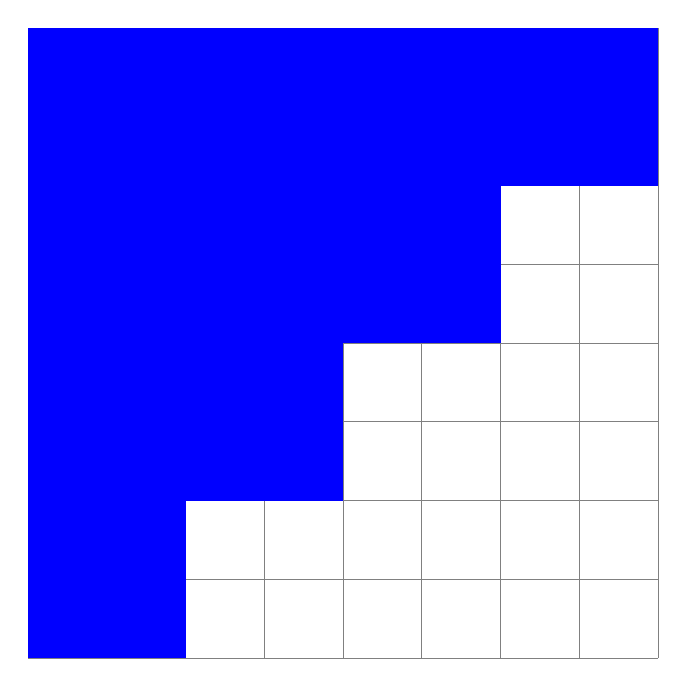
\begin{tikzpicture}
    
\def\BACKGROUNDONE{yellow}
\def\BACKGROUNDTWO{blue}
\def\CHARCOLOR{red}
	\draw[step=1.0,gray,thin] (0,0) grid (8,8);
	\fill[\BACKGROUNDTWO] (0,7) rectangle ++ (1,1);
	\fill[\BACKGROUNDTWO] (1,7) rectangle ++ (1,1);
	\fill[\BACKGROUNDTWO] (2,7) rectangle ++ (1,1);
	\fill[\BACKGROUNDTWO] (3,7) rectangle ++ (1,1);
	\fill[\BACKGROUNDTWO] (4,7) rectangle ++ (1,1);
	\fill[\BACKGROUNDTWO] (5,7) rectangle ++ (1,1);
	\fill[\BACKGROUNDTWO] (6,7) rectangle ++ (1,1);
	\fill[\BACKGROUNDTWO] (7,7) rectangle ++ (1,1);
	\fill[\BACKGROUNDTWO] (0,6) rectangle ++ (1,1);
	\fill[\BACKGROUNDTWO] (1,6) rectangle ++ (1,1);
	\fill[\BACKGROUNDTWO] (2,6) rectangle ++ (1,1);
	\fill[\BACKGROUNDTWO] (3,6) rectangle ++ (1,1);
	\fill[\BACKGROUNDTWO] (4,6) rectangle ++ (1,1);
	\fill[\BACKGROUNDTWO] (5,6) rectangle ++ (1,1);
	\fill[\BACKGROUNDTWO] (6,6) rectangle ++ (1,1);
	\fill[\BACKGROUNDTWO] (7,6) rectangle ++ (1,1);
	\fill[\BACKGROUNDTWO] (0,5) rectangle ++ (1,1);
	\fill[\BACKGROUNDTWO] (1,5) rectangle ++ (1,1);
	\fill[\BACKGROUNDTWO] (2,5) rectangle ++ (1,1);
	\fill[\BACKGROUNDTWO] (3,5) rectangle ++ (1,1);
	\fill[\BACKGROUNDTWO] (4,5) rectangle ++ (1,1);
	\fill[\BACKGROUNDTWO] (5,5) rectangle ++ (1,1);
	\fill[\BACKGROUNDTWO] (0,4) rectangle ++ (1,1);
	\fill[\BACKGROUNDTWO] (1,4) rectangle ++ (1,1);
	\fill[\BACKGROUNDTWO] (2,4) rectangle ++ (1,1);
	\fill[\BACKGROUNDTWO] (3,4) rectangle ++ (1,1);
	\fill[\BACKGROUNDTWO] (4,4) rectangle ++ (1,1);
	\fill[\BACKGROUNDTWO] (5,4) rectangle ++ (1,1);
	\fill[\BACKGROUNDTWO] (0,3) rectangle ++ (1,1);
	\fill[\BACKGROUNDTWO] (1,3) rectangle ++ (1,1);
	\fill[\BACKGROUNDTWO] (2,3) rectangle ++ (1,1);
	\fill[\BACKGROUNDTWO] (3,3) rectangle ++ (1,1);
	\fill[\BACKGROUNDTWO] (0,2) rectangle ++ (1,1);
	\fill[\BACKGROUNDTWO] (1,2) rectangle ++ (1,1);
	\fill[\BACKGROUNDTWO] (2,2) rectangle ++ (1,1);
	\fill[\BACKGROUNDTWO] (3,2) rectangle ++ (1,1);
	\fill[\BACKGROUNDTWO] (0,1) rectangle ++ (1,1);
	\fill[\BACKGROUNDTWO] (1,1) rectangle ++ (1,1);
	\fill[\BACKGROUNDTWO] (0,0) rectangle ++ (1,1);
	\fill[\BACKGROUNDTWO] (1,0) rectangle ++ (1,1);

          \end{tikzpicture}
        \end{adjustbox}
      }\caption*{\$61}
    \end{figure}
    
\end{subfigure}
    \end{adjustbox}
    \begin{adjustbox}{width=5cm,center}
\begin{subfigure}{0.12\textwidth}

    \begin{figure}[H]
      {
        \setlength{\tabcolsep}{3.0pt}
        \setlength\cmidrulewidth{\lightrulewidth} % Make cmidrule = 
        \begin{adjustbox}{width=0.5cm,center}
          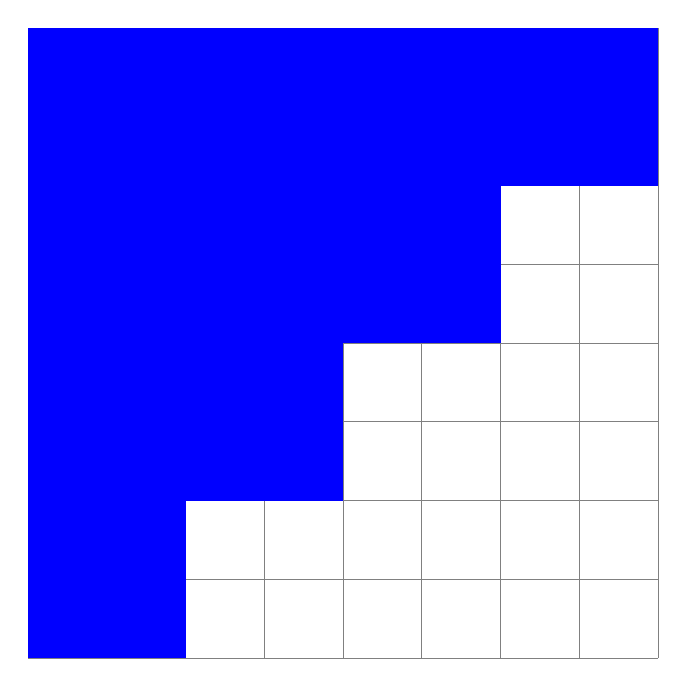
\begin{tikzpicture}
    
\def\BACKGROUNDONE{yellow}
\def\BACKGROUNDTWO{blue}
\def\CHARCOLOR{red}
	\draw[step=1.0,gray,thin] (0,0) grid (8,8);
	\fill[\BACKGROUNDTWO] (0,7) rectangle ++ (1,1);
	\fill[\BACKGROUNDTWO] (1,7) rectangle ++ (1,1);
	\fill[\BACKGROUNDTWO] (2,7) rectangle ++ (1,1);
	\fill[\BACKGROUNDTWO] (3,7) rectangle ++ (1,1);
	\fill[\BACKGROUNDTWO] (4,7) rectangle ++ (1,1);
	\fill[\BACKGROUNDTWO] (5,7) rectangle ++ (1,1);
	\fill[\BACKGROUNDTWO] (6,7) rectangle ++ (1,1);
	\fill[\BACKGROUNDTWO] (7,7) rectangle ++ (1,1);
	\fill[\BACKGROUNDTWO] (0,6) rectangle ++ (1,1);
	\fill[\BACKGROUNDTWO] (1,6) rectangle ++ (1,1);
	\fill[\BACKGROUNDTWO] (2,6) rectangle ++ (1,1);
	\fill[\BACKGROUNDTWO] (3,6) rectangle ++ (1,1);
	\fill[\BACKGROUNDTWO] (4,6) rectangle ++ (1,1);
	\fill[\BACKGROUNDTWO] (5,6) rectangle ++ (1,1);
	\fill[\BACKGROUNDTWO] (6,6) rectangle ++ (1,1);
	\fill[\BACKGROUNDTWO] (7,6) rectangle ++ (1,1);
	\fill[\BACKGROUNDTWO] (0,5) rectangle ++ (1,1);
	\fill[\BACKGROUNDTWO] (1,5) rectangle ++ (1,1);
	\fill[\BACKGROUNDTWO] (2,5) rectangle ++ (1,1);
	\fill[\BACKGROUNDTWO] (3,5) rectangle ++ (1,1);
	\fill[\BACKGROUNDTWO] (4,5) rectangle ++ (1,1);
	\fill[\BACKGROUNDTWO] (5,5) rectangle ++ (1,1);
	\fill[\BACKGROUNDTWO] (0,4) rectangle ++ (1,1);
	\fill[\BACKGROUNDTWO] (1,4) rectangle ++ (1,1);
	\fill[\BACKGROUNDTWO] (2,4) rectangle ++ (1,1);
	\fill[\BACKGROUNDTWO] (3,4) rectangle ++ (1,1);
	\fill[\BACKGROUNDTWO] (4,4) rectangle ++ (1,1);
	\fill[\BACKGROUNDTWO] (5,4) rectangle ++ (1,1);
	\fill[\BACKGROUNDTWO] (0,3) rectangle ++ (1,1);
	\fill[\BACKGROUNDTWO] (1,3) rectangle ++ (1,1);
	\fill[\BACKGROUNDTWO] (2,3) rectangle ++ (1,1);
	\fill[\BACKGROUNDTWO] (3,3) rectangle ++ (1,1);
	\fill[\BACKGROUNDTWO] (0,2) rectangle ++ (1,1);
	\fill[\BACKGROUNDTWO] (1,2) rectangle ++ (1,1);
	\fill[\BACKGROUNDTWO] (2,2) rectangle ++ (1,1);
	\fill[\BACKGROUNDTWO] (3,2) rectangle ++ (1,1);
	\fill[\BACKGROUNDTWO] (0,1) rectangle ++ (1,1);
	\fill[\BACKGROUNDTWO] (1,1) rectangle ++ (1,1);
	\fill[\BACKGROUNDTWO] (0,0) rectangle ++ (1,1);
	\fill[\BACKGROUNDTWO] (1,0) rectangle ++ (1,1);

          \end{tikzpicture}
        \end{adjustbox}
      }\caption*{\$61}
    \end{figure}
    
\end{subfigure}
\begin{subfigure}{0.12\textwidth}

    \begin{figure}[H]
      {
        \setlength{\tabcolsep}{3.0pt}
        \setlength\cmidrulewidth{\lightrulewidth} % Make cmidrule = 
        \begin{adjustbox}{width=0.5cm,center}
          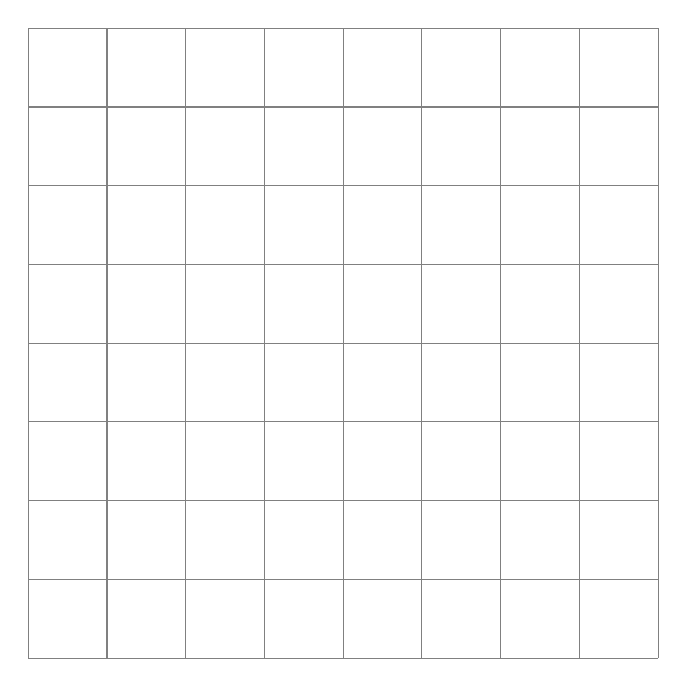
\begin{tikzpicture}
    
\def\BACKGROUNDONE{yellow}
\def\BACKGROUNDTWO{blue}
\def\CHARCOLOR{red}
	\draw[step=1.0,gray,thin] (0,0) grid (8,8);

          \end{tikzpicture}
        \end{adjustbox}
      }\caption*{\$63}
    \end{figure}
    
\end{subfigure}
    \end{adjustbox}
  }\caption[]{Characters making up the four-byte cell referenced by \icode{\$10}.}
\end{figure}

Which gives us our second cell..
\begin{figure}[H]
  {
    \begin{adjustbox}{width=2cm,center}
        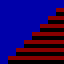
\includegraphics[width=2cm]{src/bonusphase/row21_cell1.png}%
    \end{adjustbox}
  }
\end{figure}

in the row:
\begin{figure}[H]
  {
    \setlength{\tabcolsep}{3.0pt}
    \setlength\cmidrulewidth{\heavyrulewidth} % Make cmidrule = 
    \begin{adjustbox}{width=14cm,center}
          
\includegraphics[width=10cm]{src/bonusphase/row_hex15.png}%
    \end{adjustbox}
  }
\end{figure}

The code that looks after all this is a routine we call \icode{BonusPhaseFillTopLineAfterScrollUp}
which is called every time the player scrolls up. There's an equivalent \\
\icode{BonusPhaseFillBottomLineAfterScrollDown}
for when the player scrolls down. They're nearly identical.

\begin{minipage}[b]{0.45\linewidth}
\centering
\begin{lstlisting}[basicstyle=\tiny]
BonusPhaseFillTopLineAfterScrollUp   
        LDX offsetForScrollUp
        LDY bonusPhaseMapDefinition,X
        LDA bonusPhaseMapLoPtrArray,Y
        STA bonusPhaseMapLoPtr
        LDA bonusPhaseMapHiPtrArray,Y
        STA bonusPhaseMapHiPtr

        LDY #$00
        LDX #$00
FillRowLoop
        LDA (bonusPhaseMapLoPtr),Y
        STY mapOffsetTemp
        ASL 
        CLC 
        ADC scrollLineOffset
        TAY 
        LDA cellFirstColumnArray,Y
        STA SCREEN_RAM,X
        LDA cellSecondColumnArray,Y
        STA SCREEN_RAM + LINE0_COL1,X
        LDY mapOffsetTemp
        INX 
        INX 
        INY 
        CPY #$14
        BNE FillRowLoop

        LDA scrollLineOffset
        BNE ReturnEarly

        INC offsetForScrollUp
        INC offsetForScrollDown
ReturnEarly
        RTS 
\end{lstlisting}
\end{minipage}
\hspace{0.5cm}
\begin{minipage}[b]{0.45\linewidth}
\centering
\begin{lstlisting}[basicstyle=\tiny]
BonusPhaseFillBottomLineAfterScrollDown   
        LDX offsetForScrollDown
        LDY bonusPhaseMapDefinition,X
        LDA bonusPhaseMapLoPtrArray,Y
        STA bonusPhaseMapLoPtr
        LDA bonusPhaseMapHiPtrArray,Y
        STA bonusPhaseMapHiPtr

        LDY #$00
        LDX #$00
FillRowLoop
        LDA (bonusPhaseMapLoPtr),Y
        STY mapOffsetTemp
        ASL 
        CLC 
        ADC scrollLineOffset
        TAY 
        LDA cellFirstColumnArray,Y
        STA SCREEN_RAM + LINE18_COL0,X
        LDA cellSecondColumnArray,Y
        STA SCREEN_RAM + LINE18_COL1,X
        LDY mapOffsetTemp
        INX 
        INX 
        INY 
        CPY #$14
        BNE FillRowLoop

        LDA scrollLineOffset
        BEQ FillRowLoop

        DEC offsetForScrollDown
        DEC offsetForScrollUp
        LDA offsetForScrollDown
        CMP #$FF
        BNE ReturnEarly

        LDA #$00
        STA offsetForScrollDown
        LDA #$0A
        STA offsetForScrollUp
ReturnEarly
        RTS 
\end{lstlisting}
\end{minipage}

The thing to note about this routine is that it only fills one actual line of characters
at a time, whereas as the 'rows' we've defined are two lines deep. It decides which of the
two lines its writing by using the \icode{scrollLineOffset} variable to determine which
one its writing.

\subsection{Choosing a Map}
So now that we understand how the individual rows of the map are generated, the question
arises: how do we procedurally generate entire maps? Do we just pick random rows and 
join them together? This wouldn't work well, since some rows aren't going to go well
together. The solution is to define entire map segments using the building blocks above
and let those be the building blocks we use when constructing an entire map.

If we look at our definition for the first bonus phase  again we can see it consists of arrays of 10 bytes with
each 10-byte array corresponding to a segment in the map and each byte in the array corresponding to a row in the map. 
So each 10-byte array below gives us a full 20 byte high screen of map data.

\begin{lstlisting}
bonusPhaseMapDefinition 
    .BYTE $00,$00,$00,$00,$00,$00,$00,$00,$00,$00
    .BYTE $11,$11,$11,$11,$11,$11,$11,$11,$11,$11
    .BYTE $11,$11,$11,$11,$11,$11,$11,$11,$11,$11
    .BYTE $15,$16,$16,$16,$16,$16,$16,$16,$16,$17
    .BYTE $15,$16,$16,$16,$16,$16,$16,$16,$16,$17
    .BYTE $13,$13,$13,$13,$13,$13,$13,$13,$13,$13
    .BYTE $15,$16,$16,$16,$16,$16,$16,$16,$16,$17
    .BYTE $14,$14,$00,$15,$16,$17,$00,$00,$14,$14
    .BYTE $00,$14,$14,$14,$14,$14,$14,$14,$14,$00
    .BYTE $00,$00,$00,$00,$00,$00,$00,$00,$00,$00
    .BYTE $00,$14,$14,$14,$14,$14,$14,$14,$14,$00
    .BYTE $14,$14,$00,$15,$16,$17,$00,$00,$14,$14
    .BYTE $15,$16,$16,$16,$16,$16,$16,$16,$16,$17
    .BYTE $00,$14,$14,$14,$14,$14,$14,$14,$14,$00
    .BYTE $00,$15,$16,$17,$00,$00,$15,$16,$17,$00
    .BYTE $13,$13,$13,$13,$13,$13,$13,$13,$13,$13
    .BYTE $15,$16,$16,$16,$16,$16,$16,$16,$16,$17
    .BYTE $11,$11,$11,$11,$11,$11,$11,$11,$11,$11
    .BYTE $00,$00,$00,$00,$00,$00,$00,$00,$00,$00
    .BYTE $12,$12,$12,$12,$12,$12,$12,$12,$12,$00
    .BYTE $00,$15,$16,$17,$00,$00,$15,$16,$17,$00
    .BYTE $00,$15,$16,$17,$00,$00,$15,$16,$17,$00
    .BYTE $13,$13,$13,$13,$13,$13,$13,$13,$13,$13
    .BYTE $12,$12,$12,$12,$12,$12,$12,$12,$12,$00
    .BYTE $11,$11,$11,$11,$11,$11,$11,$11,$11,$11
    .BYTE $10,$10,$10,$10,$10,$10
\end{lstlisting}

The trick is that these segments aren't themselves
generated procedurally, we defined them in advance.  We did this in \icode{bonusMapSegmentArray}
given below. We've highlighted the segments used in our map in red:

\begin{lstlisting}
bonusMapSegmentArray
        .BYTE $00,$00,$00,$00,$00,$00,$00,$00,$00,$00
        .BYTE $00,$15,$16,$17,$00,$00,$15,$16,$17,$00
        .BYTE $00,$14,$14,$14,$14,$14,$14,$14,$14,$00
        .BYTE $11,$11,$11,$11,$11,$11,$11,$11,$11,$11
        .BYTE $13,$13,$13,$13,$13,$13,$13,$13,$13,$13
        .BYTE $12,$12,$12,$12,$12,$12,$12,$12,$12,$00
        .BYTE $14,$14,$00,$15,$16,$17,$00,$00,$14,$14
        .BYTE $15,$16,$16,$16,$16,$16,$16,$16,$16,$17
        .BYTE $00,$00,$00,$00,$00,$00,$00,$00,$00,$00
        .BYTE $00,$00,$0F,$0F,$0F,$0F,$0F,$0F,$00,$00
        .BYTE $01,$01,$01,$01,$00,$00,$01,$01,$01,$01
        .BYTE $00,$00,$0B,$0B,$0B,$0C,$0C,$0C,$00,$00
        .BYTE $00,$02,$03,$04,$05,$06,$07,$08,$09,$0A
        .BYTE $02,$03,$04,$05,$05,$05,$05,$0B,$0B,$0B
        .BYTE $00,$00,$01,$01,$00,$00,$01,$01,$00,$00
        .BYTE $00,$00,$0E,$0D,$00,$00,$0E,$0D,$00,$00
        .BYTE $00,$02,$03,$04,$05,$08,$09,$0A,$0B,$00
        .BYTE $00,$00,$00,$1A,$1A,$1A,$18,$18,$18,$18
        .BYTE $00,$00,$00,$1A,$1A,$1A,$19,$19,$19,$19
        .BYTE $00,$00,$18,$18,$00,$00,$00,$00,$19,$19
        .BYTE $00,$00,$1B,$1B,$00,$00,$15,$16,$17,$00
        .BYTE $15,$16,$17,$1D,$1D,$15,$16,$17,$1D,$1D
        .BYTE $14,$14,$1E,$1E,$00,$00,$15,$16,$17,$00
        .BYTE $00,$0B,$0B,$0B,$15,$16,$17,$15,$16,$17
        .BYTE $00,$00,$1D,$1D,$1D,$1D,$1E,$1E,$1E,$1E
        .BYTE $00,$00,$20,$1F,$20,$1F,$00,$00,$11,$11
        .BYTE $00,$00,$20,$1F,$20,$1F,$20,$1F,$20,$1F
        .BYTE $00,$1E,$1E,$1E,$20,$1F,$1D,$1D,$1D,$00
        .BYTE $00,$0C,$0C,$0C,$15,$16,$17,$00,$00,$00
        .BYTE $00,$02,$03,$04,$05,$08,$09,$0A,$0B,$00
        .BYTE $00,$00,$06,$06,$06,$11,$11,$11,$00,$00
        .BYTE $00,$00,$0F,$0F,$15,$16,$17,$15,$16,$17
\end{lstlisting}

By way of example this is what the last segment in the list above looks like when 
rendered as a section of our map:

\begin{figure}[H]
  {
    \setlength{\tabcolsep}{3.0pt}
    \setlength\cmidrulewidth{\heavyrulewidth} % Make cmidrule = 
    \begin{adjustbox}{width=14cm,center}
      \begin{tabular}{cc}
        \toprule
        Index & Image\\
        \icode{\$17} & \makecell[l]{
          
\includegraphics[width=10cm]{src/bonusphase/row_hex17.png}%
        } \\
        \icode{\$16} & \makecell[l]{
          
\includegraphics[width=10cm]{src/bonusphase/row_hex16.png}%
        } \\
        \icode{\$15} & \makecell[l]{
          
\includegraphics[width=10cm]{src/bonusphase/row_hex15.png}%
        } \\
        \icode{\$17} & \makecell[l]{
          
\includegraphics[width=10cm]{src/bonusphase/row_hex17.png}%
        } \\
        \icode{\$16} & \makecell[l]{
          
\includegraphics[width=10cm]{src/bonusphase/row_hex16.png}%
        } \\
        \icode{\$15} & \makecell[l]{
          
\includegraphics[width=10cm]{src/bonusphase/row_hex15.png}%
        } \\
        \icode{\$0F} & \makecell[l]{
          
\includegraphics[width=10cm]{src/bonusphase/row_hex0F.png}%
        } \\
        \icode{\$0F} & \makecell[l]{
          
\includegraphics[width=10cm]{src/bonusphase/row_hex0F.png}%
        } \\
        \icode{\$00} & \makecell[l]{
          
\includegraphics[width=10cm]{src/bonusphase/row_hex00.png}%
        } \\
        \icode{\$00} & \makecell[l]{
          
\includegraphics[width=10cm]{src/bonusphase/row_hex00.png}%
        } \\
      \end{tabular}
    \end{adjustbox}
  }
\end{figure}

So our procedure for generating a map is simply choosing 30 of these segments in a
pseudo-random order and stacking them on top of one another!



\section{Some Very Ugly Sprites}
For some reason the gilby sprite in the bonus phase is made impossibly ugly.

\begin{figure}[H]
  {
    \setlength{\tabcolsep}{1.0pt}
    \setlength\cmidrulewidth{\heavyrulewidth} % Make cmidrule = 
    \begin{adjustbox}{width=14cm,center}
      \begin{tabular}{cccc}
        \toprule
        Please & Make & It & Stop \\
        \midrule
        \midrule
\makecell[l]{
	\begin{subfigure}{0.3\textwidth}
    \def\MULTICOLORONE{gray}
    \def\MULTICOLORTWO{white}
    \def\SPRITECOLOR{red}
		
\begin{figure}[H]
  {
    \setlength{\tabcolsep}{3.0pt}
    \setlength\cmidrulewidth{\heavyrulewidth} % Make cmidrule = 
    \begin{adjustbox}{width=3cm,center}
      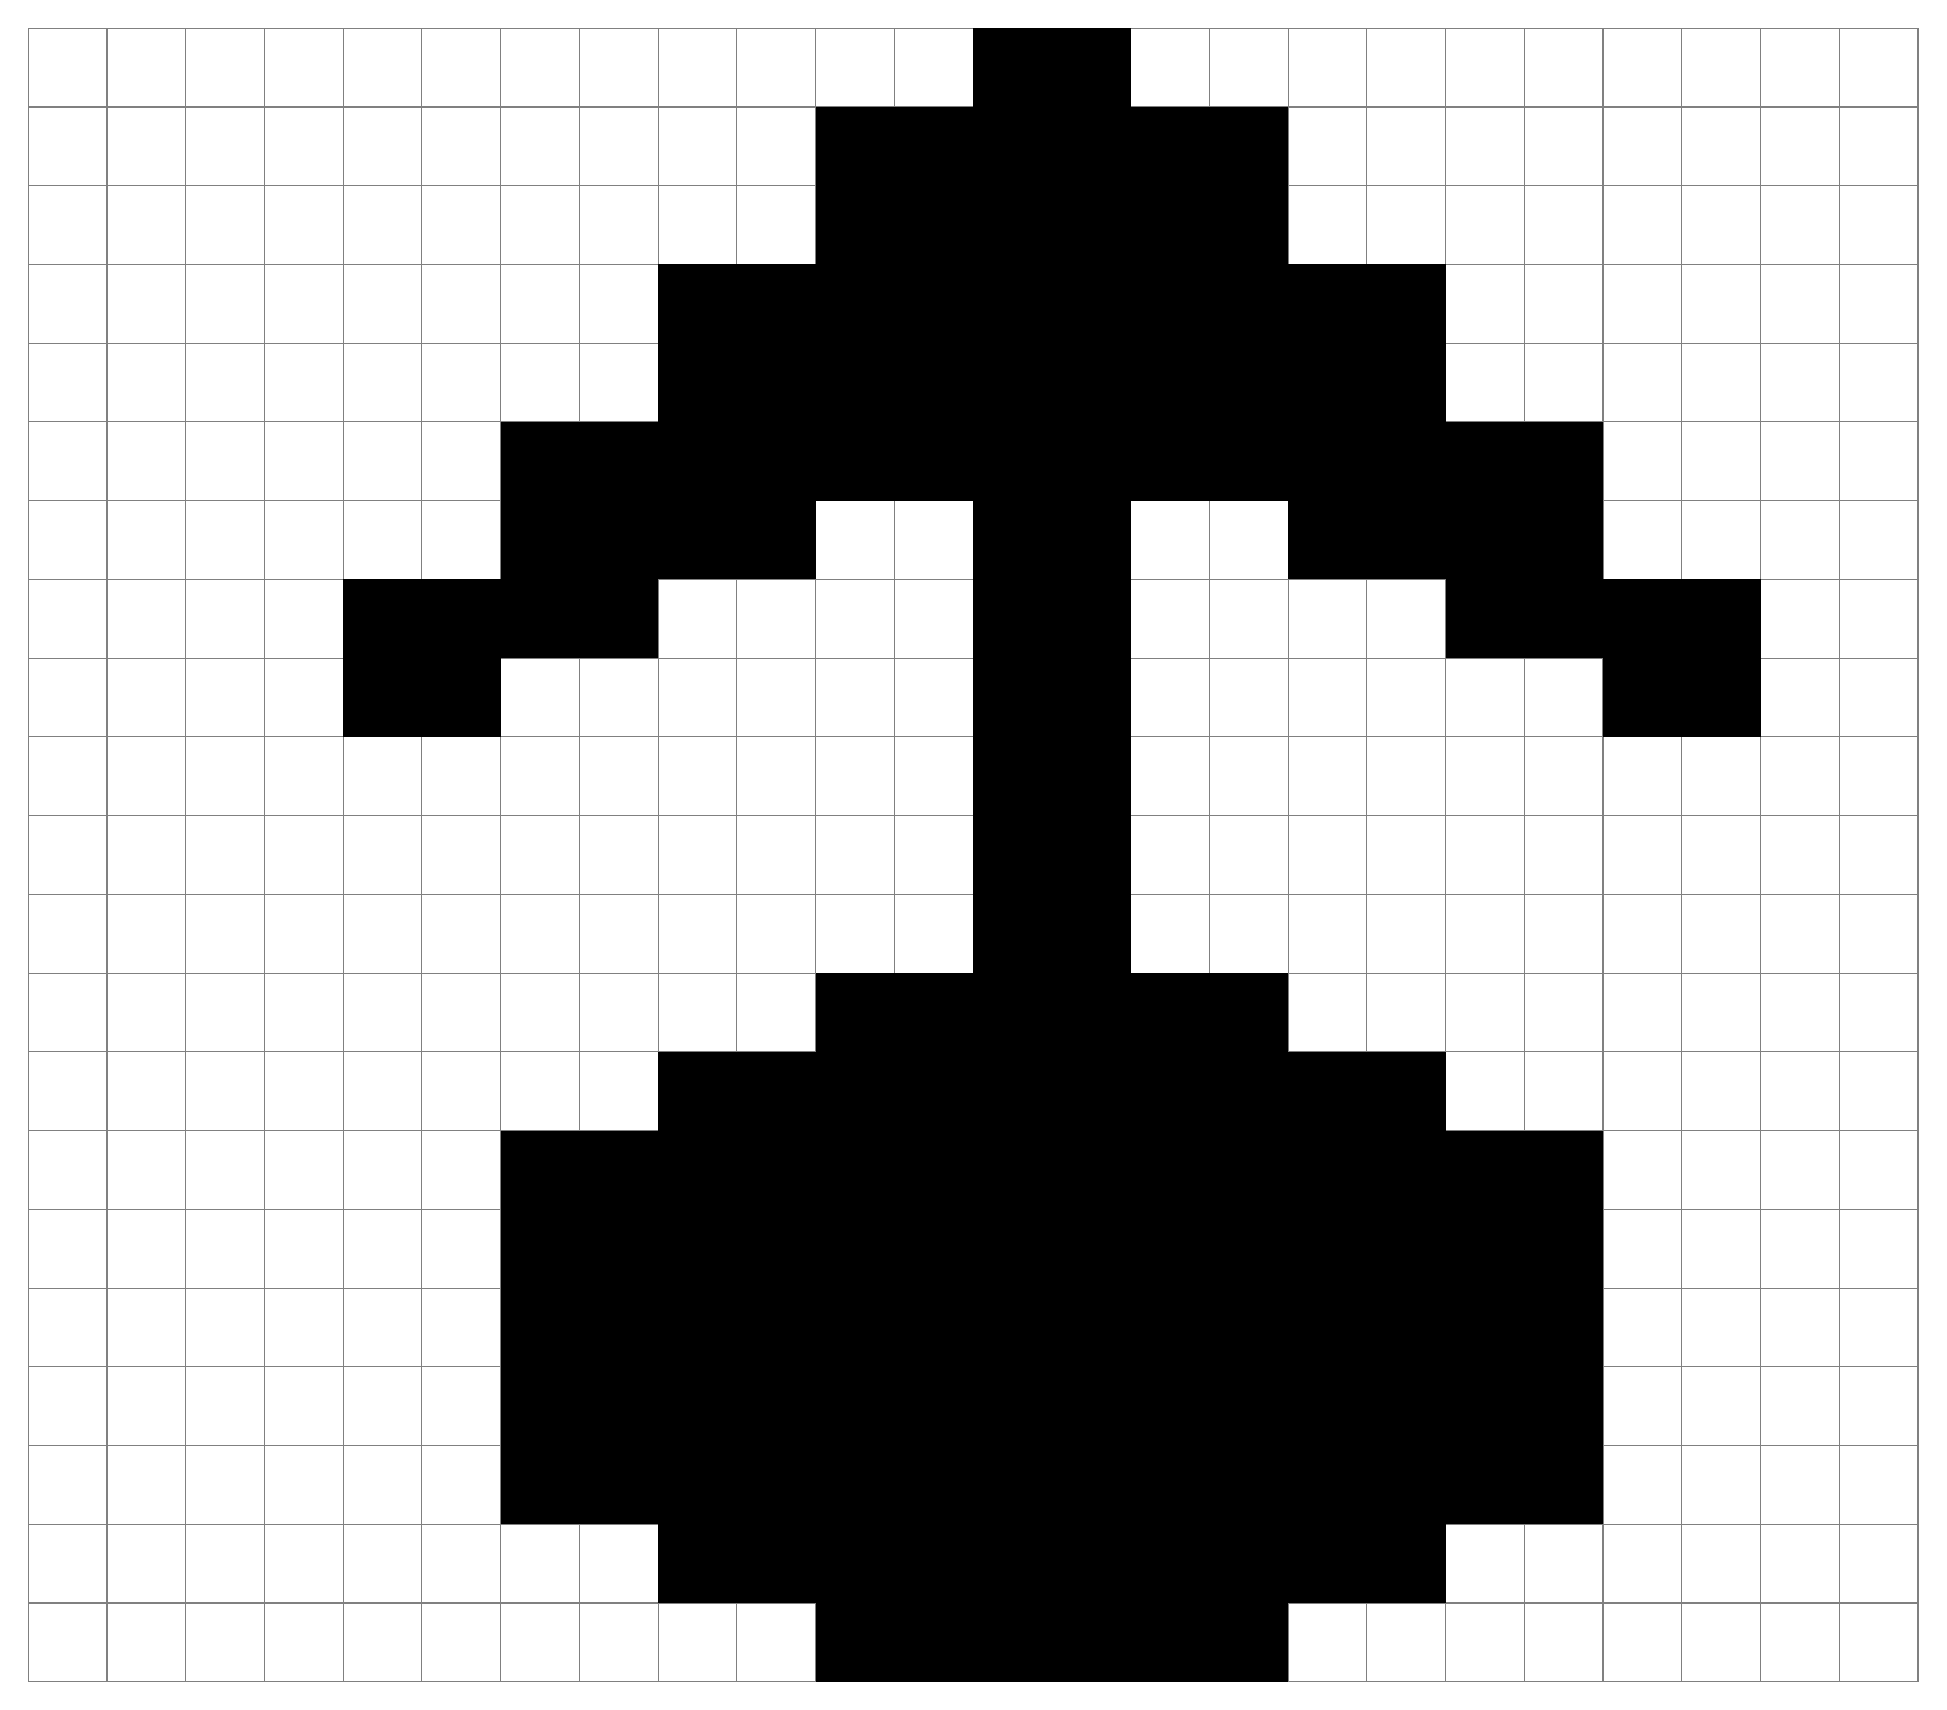
\begin{tikzpicture}

	\draw[step=1.0,gray,thin] (0,0) grid (24,21);
	\fill[\SPRITECOLOR] (12,20) rectangle ++ (1,1);
	\fill[\SPRITECOLOR] (13,20) rectangle ++ (1,1);
	\fill[\SPRITECOLOR] (10,19) rectangle ++ (1,1);
	\fill[\SPRITECOLOR] (11,19) rectangle ++ (1,1);
	\fill[\SPRITECOLOR] (12,19) rectangle ++ (1,1);
	\fill[\SPRITECOLOR] (13,19) rectangle ++ (1,1);
	\fill[\SPRITECOLOR] (14,19) rectangle ++ (1,1);
	\fill[\SPRITECOLOR] (15,19) rectangle ++ (1,1);
	\fill[\SPRITECOLOR] (10,18) rectangle ++ (1,1);
	\fill[\SPRITECOLOR] (11,18) rectangle ++ (1,1);
	\fill[\MULTICOLORONE] (12,18) rectangle ++ (1,1);
	\fill[\MULTICOLORONE] (13,18) rectangle ++ (1,1);
	\fill[\SPRITECOLOR] (14,18) rectangle ++ (1,1);
	\fill[\SPRITECOLOR] (15,18) rectangle ++ (1,1);
	\fill[\SPRITECOLOR] (8,17) rectangle ++ (1,1);
	\fill[\SPRITECOLOR] (9,17) rectangle ++ (1,1);
	\fill[\MULTICOLORONE] (10,17) rectangle ++ (1,1);
	\fill[\MULTICOLORONE] (11,17) rectangle ++ (1,1);
	\fill[\MULTICOLORONE] (12,17) rectangle ++ (1,1);
	\fill[\MULTICOLORONE] (13,17) rectangle ++ (1,1);
	\fill[\MULTICOLORONE] (14,17) rectangle ++ (1,1);
	\fill[\MULTICOLORONE] (15,17) rectangle ++ (1,1);
	\fill[\SPRITECOLOR] (16,17) rectangle ++ (1,1);
	\fill[\SPRITECOLOR] (17,17) rectangle ++ (1,1);
	\fill[\SPRITECOLOR] (8,16) rectangle ++ (1,1);
	\fill[\SPRITECOLOR] (9,16) rectangle ++ (1,1);
	\fill[\MULTICOLORONE] (10,16) rectangle ++ (1,1);
	\fill[\MULTICOLORONE] (11,16) rectangle ++ (1,1);
	\fill[\MULTICOLORONE] (12,16) rectangle ++ (1,1);
	\fill[\MULTICOLORONE] (13,16) rectangle ++ (1,1);
	\fill[\MULTICOLORONE] (14,16) rectangle ++ (1,1);
	\fill[\MULTICOLORONE] (15,16) rectangle ++ (1,1);
	\fill[\SPRITECOLOR] (16,16) rectangle ++ (1,1);
	\fill[\SPRITECOLOR] (17,16) rectangle ++ (1,1);
	\fill[\SPRITECOLOR] (6,15) rectangle ++ (1,1);
	\fill[\SPRITECOLOR] (7,15) rectangle ++ (1,1);
	\fill[\MULTICOLORONE] (8,15) rectangle ++ (1,1);
	\fill[\MULTICOLORONE] (9,15) rectangle ++ (1,1);
	\fill[\SPRITECOLOR] (10,15) rectangle ++ (1,1);
	\fill[\SPRITECOLOR] (11,15) rectangle ++ (1,1);
	\fill[\SPRITECOLOR] (12,15) rectangle ++ (1,1);
	\fill[\SPRITECOLOR] (13,15) rectangle ++ (1,1);
	\fill[\SPRITECOLOR] (14,15) rectangle ++ (1,1);
	\fill[\SPRITECOLOR] (15,15) rectangle ++ (1,1);
	\fill[\MULTICOLORONE] (16,15) rectangle ++ (1,1);
	\fill[\MULTICOLORONE] (17,15) rectangle ++ (1,1);
	\fill[\SPRITECOLOR] (18,15) rectangle ++ (1,1);
	\fill[\SPRITECOLOR] (19,15) rectangle ++ (1,1);
	\fill[\MULTICOLORONE] (6,14) rectangle ++ (1,1);
	\fill[\MULTICOLORONE] (7,14) rectangle ++ (1,1);
	\fill[\SPRITECOLOR] (8,14) rectangle ++ (1,1);
	\fill[\SPRITECOLOR] (9,14) rectangle ++ (1,1);
	\fill[\SPRITECOLOR] (12,14) rectangle ++ (1,1);
	\fill[\SPRITECOLOR] (13,14) rectangle ++ (1,1);
	\fill[\SPRITECOLOR] (16,14) rectangle ++ (1,1);
	\fill[\SPRITECOLOR] (17,14) rectangle ++ (1,1);
	\fill[\MULTICOLORONE] (18,14) rectangle ++ (1,1);
	\fill[\MULTICOLORONE] (19,14) rectangle ++ (1,1);
	\fill[\SPRITECOLOR] (4,13) rectangle ++ (1,1);
	\fill[\SPRITECOLOR] (5,13) rectangle ++ (1,1);
	\fill[\SPRITECOLOR] (6,13) rectangle ++ (1,1);
	\fill[\SPRITECOLOR] (7,13) rectangle ++ (1,1);
	\fill[\SPRITECOLOR] (12,13) rectangle ++ (1,1);
	\fill[\SPRITECOLOR] (13,13) rectangle ++ (1,1);
	\fill[\SPRITECOLOR] (18,13) rectangle ++ (1,1);
	\fill[\SPRITECOLOR] (19,13) rectangle ++ (1,1);
	\fill[\SPRITECOLOR] (20,13) rectangle ++ (1,1);
	\fill[\SPRITECOLOR] (21,13) rectangle ++ (1,1);
	\fill[\SPRITECOLOR] (4,12) rectangle ++ (1,1);
	\fill[\SPRITECOLOR] (5,12) rectangle ++ (1,1);
	\fill[\SPRITECOLOR] (12,12) rectangle ++ (1,1);
	\fill[\SPRITECOLOR] (13,12) rectangle ++ (1,1);
	\fill[\SPRITECOLOR] (20,12) rectangle ++ (1,1);
	\fill[\SPRITECOLOR] (21,12) rectangle ++ (1,1);
	\fill[\SPRITECOLOR] (12,11) rectangle ++ (1,1);
	\fill[\SPRITECOLOR] (13,11) rectangle ++ (1,1);
	\fill[\SPRITECOLOR] (12,10) rectangle ++ (1,1);
	\fill[\SPRITECOLOR] (13,10) rectangle ++ (1,1);
	\fill[\SPRITECOLOR] (12,9) rectangle ++ (1,1);
	\fill[\SPRITECOLOR] (13,9) rectangle ++ (1,1);
	\fill[\SPRITECOLOR] (10,8) rectangle ++ (1,1);
	\fill[\SPRITECOLOR] (11,8) rectangle ++ (1,1);
	\fill[\SPRITECOLOR] (12,8) rectangle ++ (1,1);
	\fill[\SPRITECOLOR] (13,8) rectangle ++ (1,1);
	\fill[\SPRITECOLOR] (14,8) rectangle ++ (1,1);
	\fill[\SPRITECOLOR] (15,8) rectangle ++ (1,1);
	\fill[\SPRITECOLOR] (8,7) rectangle ++ (1,1);
	\fill[\SPRITECOLOR] (9,7) rectangle ++ (1,1);
	\fill[\MULTICOLORTWO] (10,7) rectangle ++ (1,1);
	\fill[\MULTICOLORTWO] (11,7) rectangle ++ (1,1);
	\fill[\SPRITECOLOR] (12,7) rectangle ++ (1,1);
	\fill[\SPRITECOLOR] (13,7) rectangle ++ (1,1);
	\fill[\SPRITECOLOR] (14,7) rectangle ++ (1,1);
	\fill[\SPRITECOLOR] (15,7) rectangle ++ (1,1);
	\fill[\SPRITECOLOR] (16,7) rectangle ++ (1,1);
	\fill[\SPRITECOLOR] (17,7) rectangle ++ (1,1);
	\fill[\SPRITECOLOR] (6,6) rectangle ++ (1,1);
	\fill[\SPRITECOLOR] (7,6) rectangle ++ (1,1);
	\fill[\MULTICOLORTWO] (8,6) rectangle ++ (1,1);
	\fill[\MULTICOLORTWO] (9,6) rectangle ++ (1,1);
	\fill[\SPRITECOLOR] (10,6) rectangle ++ (1,1);
	\fill[\SPRITECOLOR] (11,6) rectangle ++ (1,1);
	\fill[\SPRITECOLOR] (12,6) rectangle ++ (1,1);
	\fill[\SPRITECOLOR] (13,6) rectangle ++ (1,1);
	\fill[\SPRITECOLOR] (14,6) rectangle ++ (1,1);
	\fill[\SPRITECOLOR] (15,6) rectangle ++ (1,1);
	\fill[\SPRITECOLOR] (16,6) rectangle ++ (1,1);
	\fill[\SPRITECOLOR] (17,6) rectangle ++ (1,1);
	\fill[\SPRITECOLOR] (18,6) rectangle ++ (1,1);
	\fill[\SPRITECOLOR] (19,6) rectangle ++ (1,1);
	\fill[\SPRITECOLOR] (6,5) rectangle ++ (1,1);
	\fill[\SPRITECOLOR] (7,5) rectangle ++ (1,1);
	\fill[\SPRITECOLOR] (8,5) rectangle ++ (1,1);
	\fill[\SPRITECOLOR] (9,5) rectangle ++ (1,1);
	\fill[\SPRITECOLOR] (10,5) rectangle ++ (1,1);
	\fill[\SPRITECOLOR] (11,5) rectangle ++ (1,1);
	\fill[\MULTICOLORONE] (12,5) rectangle ++ (1,1);
	\fill[\MULTICOLORONE] (13,5) rectangle ++ (1,1);
	\fill[\SPRITECOLOR] (14,5) rectangle ++ (1,1);
	\fill[\SPRITECOLOR] (15,5) rectangle ++ (1,1);
	\fill[\SPRITECOLOR] (16,5) rectangle ++ (1,1);
	\fill[\SPRITECOLOR] (17,5) rectangle ++ (1,1);
	\fill[\SPRITECOLOR] (18,5) rectangle ++ (1,1);
	\fill[\SPRITECOLOR] (19,5) rectangle ++ (1,1);
	\fill[\SPRITECOLOR] (6,4) rectangle ++ (1,1);
	\fill[\SPRITECOLOR] (7,4) rectangle ++ (1,1);
	\fill[\SPRITECOLOR] (8,4) rectangle ++ (1,1);
	\fill[\SPRITECOLOR] (9,4) rectangle ++ (1,1);
	\fill[\MULTICOLORONE] (10,4) rectangle ++ (1,1);
	\fill[\MULTICOLORONE] (11,4) rectangle ++ (1,1);
	\fill[\MULTICOLORONE] (12,4) rectangle ++ (1,1);
	\fill[\MULTICOLORONE] (13,4) rectangle ++ (1,1);
	\fill[\MULTICOLORONE] (14,4) rectangle ++ (1,1);
	\fill[\MULTICOLORONE] (15,4) rectangle ++ (1,1);
	\fill[\SPRITECOLOR] (16,4) rectangle ++ (1,1);
	\fill[\SPRITECOLOR] (17,4) rectangle ++ (1,1);
	\fill[\SPRITECOLOR] (18,4) rectangle ++ (1,1);
	\fill[\SPRITECOLOR] (19,4) rectangle ++ (1,1);
	\fill[\SPRITECOLOR] (6,3) rectangle ++ (1,1);
	\fill[\SPRITECOLOR] (7,3) rectangle ++ (1,1);
	\fill[\SPRITECOLOR] (8,3) rectangle ++ (1,1);
	\fill[\SPRITECOLOR] (9,3) rectangle ++ (1,1);
	\fill[\SPRITECOLOR] (10,3) rectangle ++ (1,1);
	\fill[\SPRITECOLOR] (11,3) rectangle ++ (1,1);
	\fill[\MULTICOLORONE] (12,3) rectangle ++ (1,1);
	\fill[\MULTICOLORONE] (13,3) rectangle ++ (1,1);
	\fill[\SPRITECOLOR] (14,3) rectangle ++ (1,1);
	\fill[\SPRITECOLOR] (15,3) rectangle ++ (1,1);
	\fill[\SPRITECOLOR] (16,3) rectangle ++ (1,1);
	\fill[\SPRITECOLOR] (17,3) rectangle ++ (1,1);
	\fill[\SPRITECOLOR] (18,3) rectangle ++ (1,1);
	\fill[\SPRITECOLOR] (19,3) rectangle ++ (1,1);
	\fill[\SPRITECOLOR] (6,2) rectangle ++ (1,1);
	\fill[\SPRITECOLOR] (7,2) rectangle ++ (1,1);
	\fill[\SPRITECOLOR] (8,2) rectangle ++ (1,1);
	\fill[\SPRITECOLOR] (9,2) rectangle ++ (1,1);
	\fill[\SPRITECOLOR] (10,2) rectangle ++ (1,1);
	\fill[\SPRITECOLOR] (11,2) rectangle ++ (1,1);
	\fill[\SPRITECOLOR] (12,2) rectangle ++ (1,1);
	\fill[\SPRITECOLOR] (13,2) rectangle ++ (1,1);
	\fill[\SPRITECOLOR] (14,2) rectangle ++ (1,1);
	\fill[\SPRITECOLOR] (15,2) rectangle ++ (1,1);
	\fill[\SPRITECOLOR] (16,2) rectangle ++ (1,1);
	\fill[\SPRITECOLOR] (17,2) rectangle ++ (1,1);
	\fill[\SPRITECOLOR] (18,2) rectangle ++ (1,1);
	\fill[\SPRITECOLOR] (19,2) rectangle ++ (1,1);
	\fill[\SPRITECOLOR] (8,1) rectangle ++ (1,1);
	\fill[\SPRITECOLOR] (9,1) rectangle ++ (1,1);
	\fill[\SPRITECOLOR] (10,1) rectangle ++ (1,1);
	\fill[\SPRITECOLOR] (11,1) rectangle ++ (1,1);
	\fill[\SPRITECOLOR] (12,1) rectangle ++ (1,1);
	\fill[\SPRITECOLOR] (13,1) rectangle ++ (1,1);
	\fill[\SPRITECOLOR] (14,1) rectangle ++ (1,1);
	\fill[\SPRITECOLOR] (15,1) rectangle ++ (1,1);
	\fill[\SPRITECOLOR] (16,1) rectangle ++ (1,1);
	\fill[\SPRITECOLOR] (17,1) rectangle ++ (1,1);
	\fill[\SPRITECOLOR] (10,0) rectangle ++ (1,1);
	\fill[\SPRITECOLOR] (11,0) rectangle ++ (1,1);
	\fill[\SPRITECOLOR] (12,0) rectangle ++ (1,1);
	\fill[\SPRITECOLOR] (13,0) rectangle ++ (1,1);
	\fill[\SPRITECOLOR] (14,0) rectangle ++ (1,1);
	\fill[\SPRITECOLOR] (15,0) rectangle ++ (1,1);

      \end{tikzpicture}
    \end{adjustbox}
  }\caption{UGLY\_GILBY1}
\end{figure}

	\end{subfigure}
} & 
\makecell[l]{
	\begin{subfigure}{0.3\textwidth}
    \def\MULTICOLORONE{gray}
    \def\MULTICOLORTWO{white}
    \def\SPRITECOLOR{red}
		
\begin{figure}[H]
  {
    \setlength{\tabcolsep}{3.0pt}
    \setlength\cmidrulewidth{\heavyrulewidth} % Make cmidrule = 
    \begin{adjustbox}{width=3cm,center}
      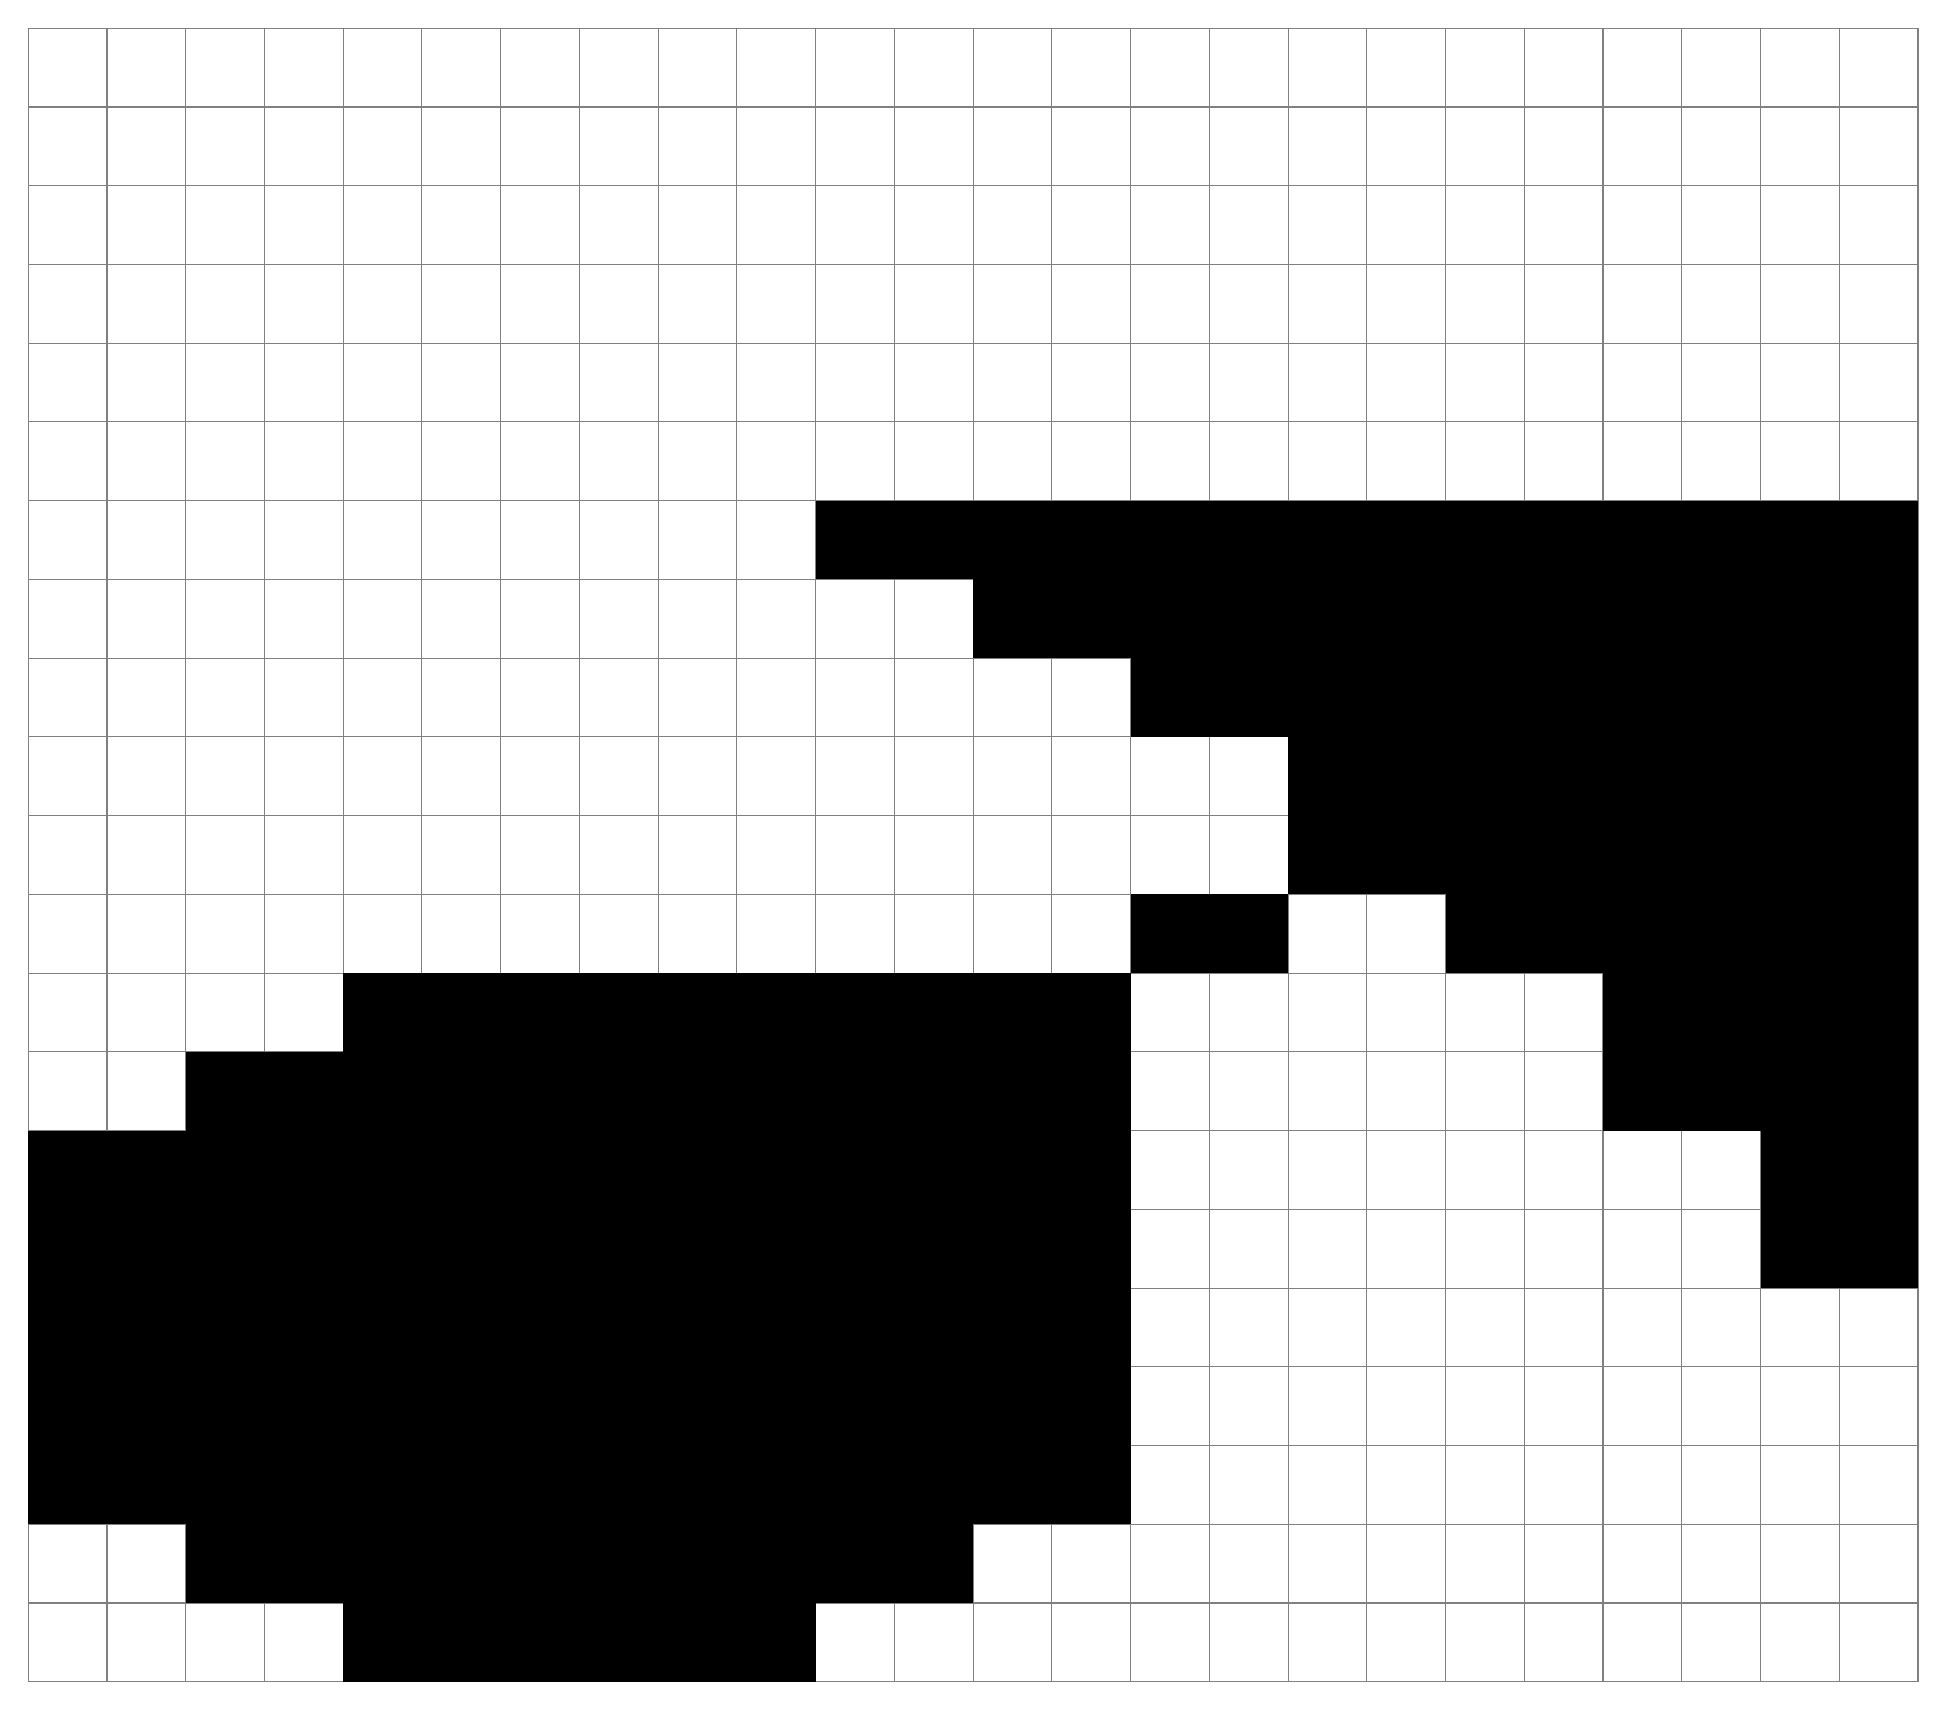
\begin{tikzpicture}

	\draw[step=1.0,gray,thin] (0,0) grid (24,21);
	\fill[\SPRITECOLOR] (10,14) rectangle ++ (1,1);
	\fill[\SPRITECOLOR] (11,14) rectangle ++ (1,1);
	\fill[\SPRITECOLOR] (12,14) rectangle ++ (1,1);
	\fill[\SPRITECOLOR] (13,14) rectangle ++ (1,1);
	\fill[\SPRITECOLOR] (14,14) rectangle ++ (1,1);
	\fill[\SPRITECOLOR] (15,14) rectangle ++ (1,1);
	\fill[\SPRITECOLOR] (16,14) rectangle ++ (1,1);
	\fill[\SPRITECOLOR] (17,14) rectangle ++ (1,1);
	\fill[\SPRITECOLOR] (18,14) rectangle ++ (1,1);
	\fill[\SPRITECOLOR] (19,14) rectangle ++ (1,1);
	\fill[\SPRITECOLOR] (20,14) rectangle ++ (1,1);
	\fill[\SPRITECOLOR] (21,14) rectangle ++ (1,1);
	\fill[\SPRITECOLOR] (22,14) rectangle ++ (1,1);
	\fill[\SPRITECOLOR] (23,14) rectangle ++ (1,1);
	\fill[\SPRITECOLOR] (12,13) rectangle ++ (1,1);
	\fill[\SPRITECOLOR] (13,13) rectangle ++ (1,1);
	\fill[\MULTICOLORONE] (14,13) rectangle ++ (1,1);
	\fill[\MULTICOLORONE] (15,13) rectangle ++ (1,1);
	\fill[\MULTICOLORONE] (16,13) rectangle ++ (1,1);
	\fill[\MULTICOLORONE] (17,13) rectangle ++ (1,1);
	\fill[\MULTICOLORONE] (18,13) rectangle ++ (1,1);
	\fill[\MULTICOLORONE] (19,13) rectangle ++ (1,1);
	\fill[\MULTICOLORONE] (20,13) rectangle ++ (1,1);
	\fill[\MULTICOLORONE] (21,13) rectangle ++ (1,1);
	\fill[\SPRITECOLOR] (22,13) rectangle ++ (1,1);
	\fill[\SPRITECOLOR] (23,13) rectangle ++ (1,1);
	\fill[\SPRITECOLOR] (14,12) rectangle ++ (1,1);
	\fill[\SPRITECOLOR] (15,12) rectangle ++ (1,1);
	\fill[\SPRITECOLOR] (16,12) rectangle ++ (1,1);
	\fill[\SPRITECOLOR] (17,12) rectangle ++ (1,1);
	\fill[\MULTICOLORONE] (18,12) rectangle ++ (1,1);
	\fill[\MULTICOLORONE] (19,12) rectangle ++ (1,1);
	\fill[\MULTICOLORONE] (20,12) rectangle ++ (1,1);
	\fill[\MULTICOLORONE] (21,12) rectangle ++ (1,1);
	\fill[\SPRITECOLOR] (22,12) rectangle ++ (1,1);
	\fill[\SPRITECOLOR] (23,12) rectangle ++ (1,1);
	\fill[\SPRITECOLOR] (16,11) rectangle ++ (1,1);
	\fill[\SPRITECOLOR] (17,11) rectangle ++ (1,1);
	\fill[\SPRITECOLOR] (18,11) rectangle ++ (1,1);
	\fill[\SPRITECOLOR] (19,11) rectangle ++ (1,1);
	\fill[\MULTICOLORONE] (20,11) rectangle ++ (1,1);
	\fill[\MULTICOLORONE] (21,11) rectangle ++ (1,1);
	\fill[\SPRITECOLOR] (22,11) rectangle ++ (1,1);
	\fill[\SPRITECOLOR] (23,11) rectangle ++ (1,1);
	\fill[\SPRITECOLOR] (16,10) rectangle ++ (1,1);
	\fill[\SPRITECOLOR] (17,10) rectangle ++ (1,1);
	\fill[\SPRITECOLOR] (18,10) rectangle ++ (1,1);
	\fill[\SPRITECOLOR] (19,10) rectangle ++ (1,1);
	\fill[\MULTICOLORONE] (20,10) rectangle ++ (1,1);
	\fill[\MULTICOLORONE] (21,10) rectangle ++ (1,1);
	\fill[\SPRITECOLOR] (22,10) rectangle ++ (1,1);
	\fill[\SPRITECOLOR] (23,10) rectangle ++ (1,1);
	\fill[\SPRITECOLOR] (14,9) rectangle ++ (1,1);
	\fill[\SPRITECOLOR] (15,9) rectangle ++ (1,1);
	\fill[\SPRITECOLOR] (18,9) rectangle ++ (1,1);
	\fill[\SPRITECOLOR] (19,9) rectangle ++ (1,1);
	\fill[\MULTICOLORONE] (20,9) rectangle ++ (1,1);
	\fill[\MULTICOLORONE] (21,9) rectangle ++ (1,1);
	\fill[\SPRITECOLOR] (22,9) rectangle ++ (1,1);
	\fill[\SPRITECOLOR] (23,9) rectangle ++ (1,1);
	\fill[\SPRITECOLOR] (4,8) rectangle ++ (1,1);
	\fill[\SPRITECOLOR] (5,8) rectangle ++ (1,1);
	\fill[\SPRITECOLOR] (6,8) rectangle ++ (1,1);
	\fill[\SPRITECOLOR] (7,8) rectangle ++ (1,1);
	\fill[\SPRITECOLOR] (8,8) rectangle ++ (1,1);
	\fill[\SPRITECOLOR] (9,8) rectangle ++ (1,1);
	\fill[\SPRITECOLOR] (10,8) rectangle ++ (1,1);
	\fill[\SPRITECOLOR] (11,8) rectangle ++ (1,1);
	\fill[\SPRITECOLOR] (12,8) rectangle ++ (1,1);
	\fill[\SPRITECOLOR] (13,8) rectangle ++ (1,1);
	\fill[\SPRITECOLOR] (20,8) rectangle ++ (1,1);
	\fill[\SPRITECOLOR] (21,8) rectangle ++ (1,1);
	\fill[\SPRITECOLOR] (22,8) rectangle ++ (1,1);
	\fill[\SPRITECOLOR] (23,8) rectangle ++ (1,1);
	\fill[\SPRITECOLOR] (2,7) rectangle ++ (1,1);
	\fill[\SPRITECOLOR] (3,7) rectangle ++ (1,1);
	\fill[\MULTICOLORTWO] (4,7) rectangle ++ (1,1);
	\fill[\MULTICOLORTWO] (5,7) rectangle ++ (1,1);
	\fill[\SPRITECOLOR] (6,7) rectangle ++ (1,1);
	\fill[\SPRITECOLOR] (7,7) rectangle ++ (1,1);
	\fill[\SPRITECOLOR] (8,7) rectangle ++ (1,1);
	\fill[\SPRITECOLOR] (9,7) rectangle ++ (1,1);
	\fill[\SPRITECOLOR] (10,7) rectangle ++ (1,1);
	\fill[\SPRITECOLOR] (11,7) rectangle ++ (1,1);
	\fill[\SPRITECOLOR] (12,7) rectangle ++ (1,1);
	\fill[\SPRITECOLOR] (13,7) rectangle ++ (1,1);
	\fill[\SPRITECOLOR] (20,7) rectangle ++ (1,1);
	\fill[\SPRITECOLOR] (21,7) rectangle ++ (1,1);
	\fill[\SPRITECOLOR] (22,7) rectangle ++ (1,1);
	\fill[\SPRITECOLOR] (23,7) rectangle ++ (1,1);
	\fill[\SPRITECOLOR] (0,6) rectangle ++ (1,1);
	\fill[\SPRITECOLOR] (1,6) rectangle ++ (1,1);
	\fill[\MULTICOLORTWO] (2,6) rectangle ++ (1,1);
	\fill[\MULTICOLORTWO] (3,6) rectangle ++ (1,1);
	\fill[\SPRITECOLOR] (4,6) rectangle ++ (1,1);
	\fill[\SPRITECOLOR] (5,6) rectangle ++ (1,1);
	\fill[\SPRITECOLOR] (6,6) rectangle ++ (1,1);
	\fill[\SPRITECOLOR] (7,6) rectangle ++ (1,1);
	\fill[\SPRITECOLOR] (8,6) rectangle ++ (1,1);
	\fill[\SPRITECOLOR] (9,6) rectangle ++ (1,1);
	\fill[\SPRITECOLOR] (10,6) rectangle ++ (1,1);
	\fill[\SPRITECOLOR] (11,6) rectangle ++ (1,1);
	\fill[\SPRITECOLOR] (12,6) rectangle ++ (1,1);
	\fill[\SPRITECOLOR] (13,6) rectangle ++ (1,1);
	\fill[\SPRITECOLOR] (22,6) rectangle ++ (1,1);
	\fill[\SPRITECOLOR] (23,6) rectangle ++ (1,1);
	\fill[\SPRITECOLOR] (0,5) rectangle ++ (1,1);
	\fill[\SPRITECOLOR] (1,5) rectangle ++ (1,1);
	\fill[\SPRITECOLOR] (2,5) rectangle ++ (1,1);
	\fill[\SPRITECOLOR] (3,5) rectangle ++ (1,1);
	\fill[\SPRITECOLOR] (4,5) rectangle ++ (1,1);
	\fill[\SPRITECOLOR] (5,5) rectangle ++ (1,1);
	\fill[\MULTICOLORONE] (6,5) rectangle ++ (1,1);
	\fill[\MULTICOLORONE] (7,5) rectangle ++ (1,1);
	\fill[\SPRITECOLOR] (8,5) rectangle ++ (1,1);
	\fill[\SPRITECOLOR] (9,5) rectangle ++ (1,1);
	\fill[\SPRITECOLOR] (10,5) rectangle ++ (1,1);
	\fill[\SPRITECOLOR] (11,5) rectangle ++ (1,1);
	\fill[\SPRITECOLOR] (12,5) rectangle ++ (1,1);
	\fill[\SPRITECOLOR] (13,5) rectangle ++ (1,1);
	\fill[\SPRITECOLOR] (22,5) rectangle ++ (1,1);
	\fill[\SPRITECOLOR] (23,5) rectangle ++ (1,1);
	\fill[\SPRITECOLOR] (0,4) rectangle ++ (1,1);
	\fill[\SPRITECOLOR] (1,4) rectangle ++ (1,1);
	\fill[\SPRITECOLOR] (2,4) rectangle ++ (1,1);
	\fill[\SPRITECOLOR] (3,4) rectangle ++ (1,1);
	\fill[\MULTICOLORONE] (4,4) rectangle ++ (1,1);
	\fill[\MULTICOLORONE] (5,4) rectangle ++ (1,1);
	\fill[\MULTICOLORONE] (6,4) rectangle ++ (1,1);
	\fill[\MULTICOLORONE] (7,4) rectangle ++ (1,1);
	\fill[\MULTICOLORONE] (8,4) rectangle ++ (1,1);
	\fill[\MULTICOLORONE] (9,4) rectangle ++ (1,1);
	\fill[\SPRITECOLOR] (10,4) rectangle ++ (1,1);
	\fill[\SPRITECOLOR] (11,4) rectangle ++ (1,1);
	\fill[\SPRITECOLOR] (12,4) rectangle ++ (1,1);
	\fill[\SPRITECOLOR] (13,4) rectangle ++ (1,1);
	\fill[\SPRITECOLOR] (0,3) rectangle ++ (1,1);
	\fill[\SPRITECOLOR] (1,3) rectangle ++ (1,1);
	\fill[\SPRITECOLOR] (2,3) rectangle ++ (1,1);
	\fill[\SPRITECOLOR] (3,3) rectangle ++ (1,1);
	\fill[\SPRITECOLOR] (4,3) rectangle ++ (1,1);
	\fill[\SPRITECOLOR] (5,3) rectangle ++ (1,1);
	\fill[\MULTICOLORONE] (6,3) rectangle ++ (1,1);
	\fill[\MULTICOLORONE] (7,3) rectangle ++ (1,1);
	\fill[\SPRITECOLOR] (8,3) rectangle ++ (1,1);
	\fill[\SPRITECOLOR] (9,3) rectangle ++ (1,1);
	\fill[\SPRITECOLOR] (10,3) rectangle ++ (1,1);
	\fill[\SPRITECOLOR] (11,3) rectangle ++ (1,1);
	\fill[\SPRITECOLOR] (12,3) rectangle ++ (1,1);
	\fill[\SPRITECOLOR] (13,3) rectangle ++ (1,1);
	\fill[\SPRITECOLOR] (0,2) rectangle ++ (1,1);
	\fill[\SPRITECOLOR] (1,2) rectangle ++ (1,1);
	\fill[\SPRITECOLOR] (2,2) rectangle ++ (1,1);
	\fill[\SPRITECOLOR] (3,2) rectangle ++ (1,1);
	\fill[\SPRITECOLOR] (4,2) rectangle ++ (1,1);
	\fill[\SPRITECOLOR] (5,2) rectangle ++ (1,1);
	\fill[\SPRITECOLOR] (6,2) rectangle ++ (1,1);
	\fill[\SPRITECOLOR] (7,2) rectangle ++ (1,1);
	\fill[\SPRITECOLOR] (8,2) rectangle ++ (1,1);
	\fill[\SPRITECOLOR] (9,2) rectangle ++ (1,1);
	\fill[\SPRITECOLOR] (10,2) rectangle ++ (1,1);
	\fill[\SPRITECOLOR] (11,2) rectangle ++ (1,1);
	\fill[\SPRITECOLOR] (12,2) rectangle ++ (1,1);
	\fill[\SPRITECOLOR] (13,2) rectangle ++ (1,1);
	\fill[\SPRITECOLOR] (2,1) rectangle ++ (1,1);
	\fill[\SPRITECOLOR] (3,1) rectangle ++ (1,1);
	\fill[\SPRITECOLOR] (4,1) rectangle ++ (1,1);
	\fill[\SPRITECOLOR] (5,1) rectangle ++ (1,1);
	\fill[\SPRITECOLOR] (6,1) rectangle ++ (1,1);
	\fill[\SPRITECOLOR] (7,1) rectangle ++ (1,1);
	\fill[\SPRITECOLOR] (8,1) rectangle ++ (1,1);
	\fill[\SPRITECOLOR] (9,1) rectangle ++ (1,1);
	\fill[\SPRITECOLOR] (10,1) rectangle ++ (1,1);
	\fill[\SPRITECOLOR] (11,1) rectangle ++ (1,1);
	\fill[\SPRITECOLOR] (4,0) rectangle ++ (1,1);
	\fill[\SPRITECOLOR] (5,0) rectangle ++ (1,1);
	\fill[\SPRITECOLOR] (6,0) rectangle ++ (1,1);
	\fill[\SPRITECOLOR] (7,0) rectangle ++ (1,1);
	\fill[\SPRITECOLOR] (8,0) rectangle ++ (1,1);
	\fill[\SPRITECOLOR] (9,0) rectangle ++ (1,1);

      \end{tikzpicture}
    \end{adjustbox}
  }\caption{UGLY\_GILBY2}
\end{figure}

	\end{subfigure}
} & 
\makecell[l]{
	\begin{subfigure}{0.3\textwidth}
    \def\MULTICOLORONE{gray}
    \def\MULTICOLORTWO{white}
    \def\SPRITECOLOR{red}
		
\begin{figure}[H]
  {
    \setlength{\tabcolsep}{3.0pt}
    \setlength\cmidrulewidth{\heavyrulewidth} % Make cmidrule = 
    \begin{adjustbox}{width=3cm,center}
      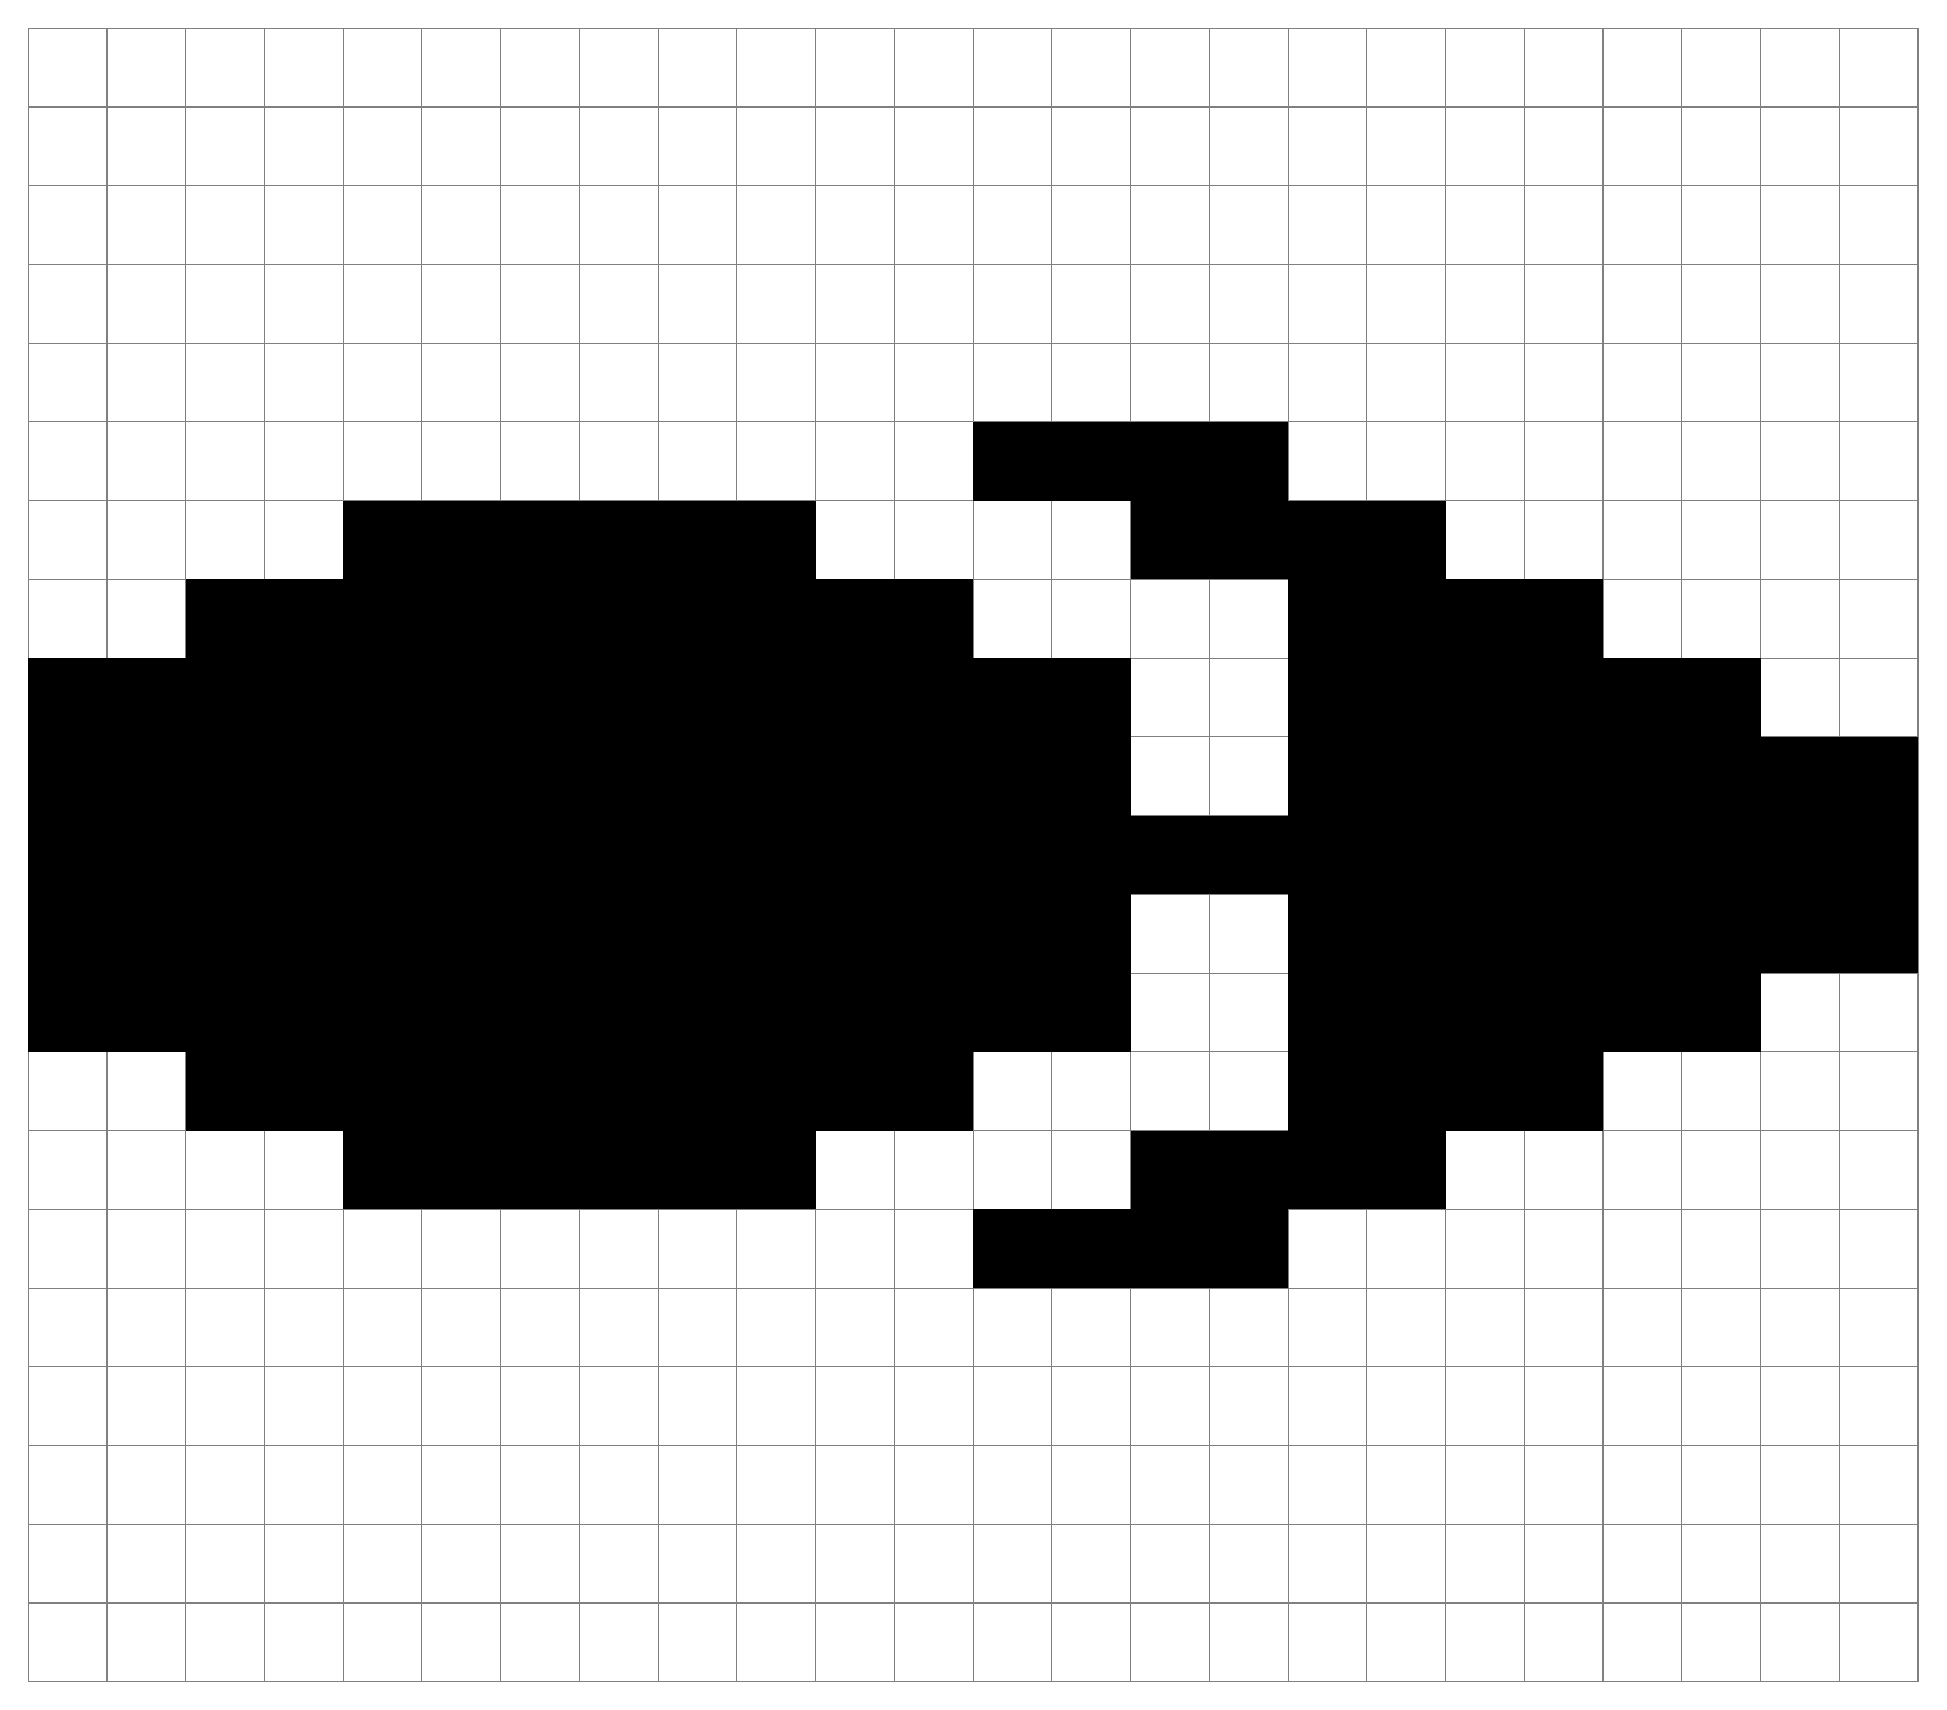
\begin{tikzpicture}

	\draw[step=1.0,gray,thin] (0,0) grid (24,21);
	\fill[\SPRITECOLOR] (12,15) rectangle ++ (1,1);
	\fill[\SPRITECOLOR] (13,15) rectangle ++ (1,1);
	\fill[\SPRITECOLOR] (14,15) rectangle ++ (1,1);
	\fill[\SPRITECOLOR] (15,15) rectangle ++ (1,1);
	\fill[\SPRITECOLOR] (4,14) rectangle ++ (1,1);
	\fill[\SPRITECOLOR] (5,14) rectangle ++ (1,1);
	\fill[\SPRITECOLOR] (6,14) rectangle ++ (1,1);
	\fill[\SPRITECOLOR] (7,14) rectangle ++ (1,1);
	\fill[\SPRITECOLOR] (8,14) rectangle ++ (1,1);
	\fill[\SPRITECOLOR] (9,14) rectangle ++ (1,1);
	\fill[\SPRITECOLOR] (14,14) rectangle ++ (1,1);
	\fill[\SPRITECOLOR] (15,14) rectangle ++ (1,1);
	\fill[\SPRITECOLOR] (16,14) rectangle ++ (1,1);
	\fill[\SPRITECOLOR] (17,14) rectangle ++ (1,1);
	\fill[\SPRITECOLOR] (2,13) rectangle ++ (1,1);
	\fill[\SPRITECOLOR] (3,13) rectangle ++ (1,1);
	\fill[\MULTICOLORTWO] (4,13) rectangle ++ (1,1);
	\fill[\MULTICOLORTWO] (5,13) rectangle ++ (1,1);
	\fill[\SPRITECOLOR] (6,13) rectangle ++ (1,1);
	\fill[\SPRITECOLOR] (7,13) rectangle ++ (1,1);
	\fill[\SPRITECOLOR] (8,13) rectangle ++ (1,1);
	\fill[\SPRITECOLOR] (9,13) rectangle ++ (1,1);
	\fill[\SPRITECOLOR] (10,13) rectangle ++ (1,1);
	\fill[\SPRITECOLOR] (11,13) rectangle ++ (1,1);
	\fill[\MULTICOLORONE] (16,13) rectangle ++ (1,1);
	\fill[\MULTICOLORONE] (17,13) rectangle ++ (1,1);
	\fill[\SPRITECOLOR] (18,13) rectangle ++ (1,1);
	\fill[\SPRITECOLOR] (19,13) rectangle ++ (1,1);
	\fill[\SPRITECOLOR] (0,12) rectangle ++ (1,1);
	\fill[\SPRITECOLOR] (1,12) rectangle ++ (1,1);
	\fill[\MULTICOLORTWO] (2,12) rectangle ++ (1,1);
	\fill[\MULTICOLORTWO] (3,12) rectangle ++ (1,1);
	\fill[\SPRITECOLOR] (4,12) rectangle ++ (1,1);
	\fill[\SPRITECOLOR] (5,12) rectangle ++ (1,1);
	\fill[\SPRITECOLOR] (6,12) rectangle ++ (1,1);
	\fill[\SPRITECOLOR] (7,12) rectangle ++ (1,1);
	\fill[\SPRITECOLOR] (8,12) rectangle ++ (1,1);
	\fill[\SPRITECOLOR] (9,12) rectangle ++ (1,1);
	\fill[\SPRITECOLOR] (10,12) rectangle ++ (1,1);
	\fill[\SPRITECOLOR] (11,12) rectangle ++ (1,1);
	\fill[\SPRITECOLOR] (12,12) rectangle ++ (1,1);
	\fill[\SPRITECOLOR] (13,12) rectangle ++ (1,1);
	\fill[\SPRITECOLOR] (16,12) rectangle ++ (1,1);
	\fill[\SPRITECOLOR] (17,12) rectangle ++ (1,1);
	\fill[\MULTICOLORONE] (18,12) rectangle ++ (1,1);
	\fill[\MULTICOLORONE] (19,12) rectangle ++ (1,1);
	\fill[\SPRITECOLOR] (20,12) rectangle ++ (1,1);
	\fill[\SPRITECOLOR] (21,12) rectangle ++ (1,1);
	\fill[\SPRITECOLOR] (0,11) rectangle ++ (1,1);
	\fill[\SPRITECOLOR] (1,11) rectangle ++ (1,1);
	\fill[\SPRITECOLOR] (2,11) rectangle ++ (1,1);
	\fill[\SPRITECOLOR] (3,11) rectangle ++ (1,1);
	\fill[\SPRITECOLOR] (4,11) rectangle ++ (1,1);
	\fill[\SPRITECOLOR] (5,11) rectangle ++ (1,1);
	\fill[\MULTICOLORONE] (6,11) rectangle ++ (1,1);
	\fill[\MULTICOLORONE] (7,11) rectangle ++ (1,1);
	\fill[\SPRITECOLOR] (8,11) rectangle ++ (1,1);
	\fill[\SPRITECOLOR] (9,11) rectangle ++ (1,1);
	\fill[\SPRITECOLOR] (10,11) rectangle ++ (1,1);
	\fill[\SPRITECOLOR] (11,11) rectangle ++ (1,1);
	\fill[\SPRITECOLOR] (12,11) rectangle ++ (1,1);
	\fill[\SPRITECOLOR] (13,11) rectangle ++ (1,1);
	\fill[\SPRITECOLOR] (16,11) rectangle ++ (1,1);
	\fill[\SPRITECOLOR] (17,11) rectangle ++ (1,1);
	\fill[\MULTICOLORONE] (18,11) rectangle ++ (1,1);
	\fill[\MULTICOLORONE] (19,11) rectangle ++ (1,1);
	\fill[\MULTICOLORONE] (20,11) rectangle ++ (1,1);
	\fill[\MULTICOLORONE] (21,11) rectangle ++ (1,1);
	\fill[\SPRITECOLOR] (22,11) rectangle ++ (1,1);
	\fill[\SPRITECOLOR] (23,11) rectangle ++ (1,1);
	\fill[\SPRITECOLOR] (0,10) rectangle ++ (1,1);
	\fill[\SPRITECOLOR] (1,10) rectangle ++ (1,1);
	\fill[\SPRITECOLOR] (2,10) rectangle ++ (1,1);
	\fill[\SPRITECOLOR] (3,10) rectangle ++ (1,1);
	\fill[\MULTICOLORONE] (4,10) rectangle ++ (1,1);
	\fill[\MULTICOLORONE] (5,10) rectangle ++ (1,1);
	\fill[\MULTICOLORONE] (6,10) rectangle ++ (1,1);
	\fill[\MULTICOLORONE] (7,10) rectangle ++ (1,1);
	\fill[\MULTICOLORONE] (8,10) rectangle ++ (1,1);
	\fill[\MULTICOLORONE] (9,10) rectangle ++ (1,1);
	\fill[\SPRITECOLOR] (10,10) rectangle ++ (1,1);
	\fill[\SPRITECOLOR] (11,10) rectangle ++ (1,1);
	\fill[\SPRITECOLOR] (12,10) rectangle ++ (1,1);
	\fill[\SPRITECOLOR] (13,10) rectangle ++ (1,1);
	\fill[\SPRITECOLOR] (14,10) rectangle ++ (1,1);
	\fill[\SPRITECOLOR] (15,10) rectangle ++ (1,1);
	\fill[\SPRITECOLOR] (16,10) rectangle ++ (1,1);
	\fill[\SPRITECOLOR] (17,10) rectangle ++ (1,1);
	\fill[\MULTICOLORONE] (18,10) rectangle ++ (1,1);
	\fill[\MULTICOLORONE] (19,10) rectangle ++ (1,1);
	\fill[\MULTICOLORONE] (20,10) rectangle ++ (1,1);
	\fill[\MULTICOLORONE] (21,10) rectangle ++ (1,1);
	\fill[\SPRITECOLOR] (22,10) rectangle ++ (1,1);
	\fill[\SPRITECOLOR] (23,10) rectangle ++ (1,1);
	\fill[\SPRITECOLOR] (0,9) rectangle ++ (1,1);
	\fill[\SPRITECOLOR] (1,9) rectangle ++ (1,1);
	\fill[\SPRITECOLOR] (2,9) rectangle ++ (1,1);
	\fill[\SPRITECOLOR] (3,9) rectangle ++ (1,1);
	\fill[\SPRITECOLOR] (4,9) rectangle ++ (1,1);
	\fill[\SPRITECOLOR] (5,9) rectangle ++ (1,1);
	\fill[\MULTICOLORONE] (6,9) rectangle ++ (1,1);
	\fill[\MULTICOLORONE] (7,9) rectangle ++ (1,1);
	\fill[\SPRITECOLOR] (8,9) rectangle ++ (1,1);
	\fill[\SPRITECOLOR] (9,9) rectangle ++ (1,1);
	\fill[\SPRITECOLOR] (10,9) rectangle ++ (1,1);
	\fill[\SPRITECOLOR] (11,9) rectangle ++ (1,1);
	\fill[\SPRITECOLOR] (12,9) rectangle ++ (1,1);
	\fill[\SPRITECOLOR] (13,9) rectangle ++ (1,1);
	\fill[\SPRITECOLOR] (16,9) rectangle ++ (1,1);
	\fill[\SPRITECOLOR] (17,9) rectangle ++ (1,1);
	\fill[\MULTICOLORONE] (18,9) rectangle ++ (1,1);
	\fill[\MULTICOLORONE] (19,9) rectangle ++ (1,1);
	\fill[\MULTICOLORONE] (20,9) rectangle ++ (1,1);
	\fill[\MULTICOLORONE] (21,9) rectangle ++ (1,1);
	\fill[\SPRITECOLOR] (22,9) rectangle ++ (1,1);
	\fill[\SPRITECOLOR] (23,9) rectangle ++ (1,1);
	\fill[\SPRITECOLOR] (0,8) rectangle ++ (1,1);
	\fill[\SPRITECOLOR] (1,8) rectangle ++ (1,1);
	\fill[\SPRITECOLOR] (2,8) rectangle ++ (1,1);
	\fill[\SPRITECOLOR] (3,8) rectangle ++ (1,1);
	\fill[\SPRITECOLOR] (4,8) rectangle ++ (1,1);
	\fill[\SPRITECOLOR] (5,8) rectangle ++ (1,1);
	\fill[\SPRITECOLOR] (6,8) rectangle ++ (1,1);
	\fill[\SPRITECOLOR] (7,8) rectangle ++ (1,1);
	\fill[\SPRITECOLOR] (8,8) rectangle ++ (1,1);
	\fill[\SPRITECOLOR] (9,8) rectangle ++ (1,1);
	\fill[\SPRITECOLOR] (10,8) rectangle ++ (1,1);
	\fill[\SPRITECOLOR] (11,8) rectangle ++ (1,1);
	\fill[\SPRITECOLOR] (12,8) rectangle ++ (1,1);
	\fill[\SPRITECOLOR] (13,8) rectangle ++ (1,1);
	\fill[\SPRITECOLOR] (16,8) rectangle ++ (1,1);
	\fill[\SPRITECOLOR] (17,8) rectangle ++ (1,1);
	\fill[\MULTICOLORONE] (18,8) rectangle ++ (1,1);
	\fill[\MULTICOLORONE] (19,8) rectangle ++ (1,1);
	\fill[\SPRITECOLOR] (20,8) rectangle ++ (1,1);
	\fill[\SPRITECOLOR] (21,8) rectangle ++ (1,1);
	\fill[\SPRITECOLOR] (2,7) rectangle ++ (1,1);
	\fill[\SPRITECOLOR] (3,7) rectangle ++ (1,1);
	\fill[\SPRITECOLOR] (4,7) rectangle ++ (1,1);
	\fill[\SPRITECOLOR] (5,7) rectangle ++ (1,1);
	\fill[\SPRITECOLOR] (6,7) rectangle ++ (1,1);
	\fill[\SPRITECOLOR] (7,7) rectangle ++ (1,1);
	\fill[\SPRITECOLOR] (8,7) rectangle ++ (1,1);
	\fill[\SPRITECOLOR] (9,7) rectangle ++ (1,1);
	\fill[\SPRITECOLOR] (10,7) rectangle ++ (1,1);
	\fill[\SPRITECOLOR] (11,7) rectangle ++ (1,1);
	\fill[\MULTICOLORONE] (16,7) rectangle ++ (1,1);
	\fill[\MULTICOLORONE] (17,7) rectangle ++ (1,1);
	\fill[\SPRITECOLOR] (18,7) rectangle ++ (1,1);
	\fill[\SPRITECOLOR] (19,7) rectangle ++ (1,1);
	\fill[\SPRITECOLOR] (4,6) rectangle ++ (1,1);
	\fill[\SPRITECOLOR] (5,6) rectangle ++ (1,1);
	\fill[\SPRITECOLOR] (6,6) rectangle ++ (1,1);
	\fill[\SPRITECOLOR] (7,6) rectangle ++ (1,1);
	\fill[\SPRITECOLOR] (8,6) rectangle ++ (1,1);
	\fill[\SPRITECOLOR] (9,6) rectangle ++ (1,1);
	\fill[\SPRITECOLOR] (14,6) rectangle ++ (1,1);
	\fill[\SPRITECOLOR] (15,6) rectangle ++ (1,1);
	\fill[\SPRITECOLOR] (16,6) rectangle ++ (1,1);
	\fill[\SPRITECOLOR] (17,6) rectangle ++ (1,1);
	\fill[\SPRITECOLOR] (12,5) rectangle ++ (1,1);
	\fill[\SPRITECOLOR] (13,5) rectangle ++ (1,1);
	\fill[\SPRITECOLOR] (14,5) rectangle ++ (1,1);
	\fill[\SPRITECOLOR] (15,5) rectangle ++ (1,1);

      \end{tikzpicture}
    \end{adjustbox}
  }\caption{UGLY\_GILBY3}
\end{figure}

	\end{subfigure}
} & 
\makecell[l]{
	\begin{subfigure}{0.3\textwidth}
    \def\MULTICOLORONE{gray}
    \def\MULTICOLORTWO{white}
    \def\SPRITECOLOR{red}
		
\begin{figure}[H]
  {
    \setlength{\tabcolsep}{3.0pt}
    \setlength\cmidrulewidth{\heavyrulewidth} % Make cmidrule = 
    \begin{adjustbox}{width=3cm,center}
      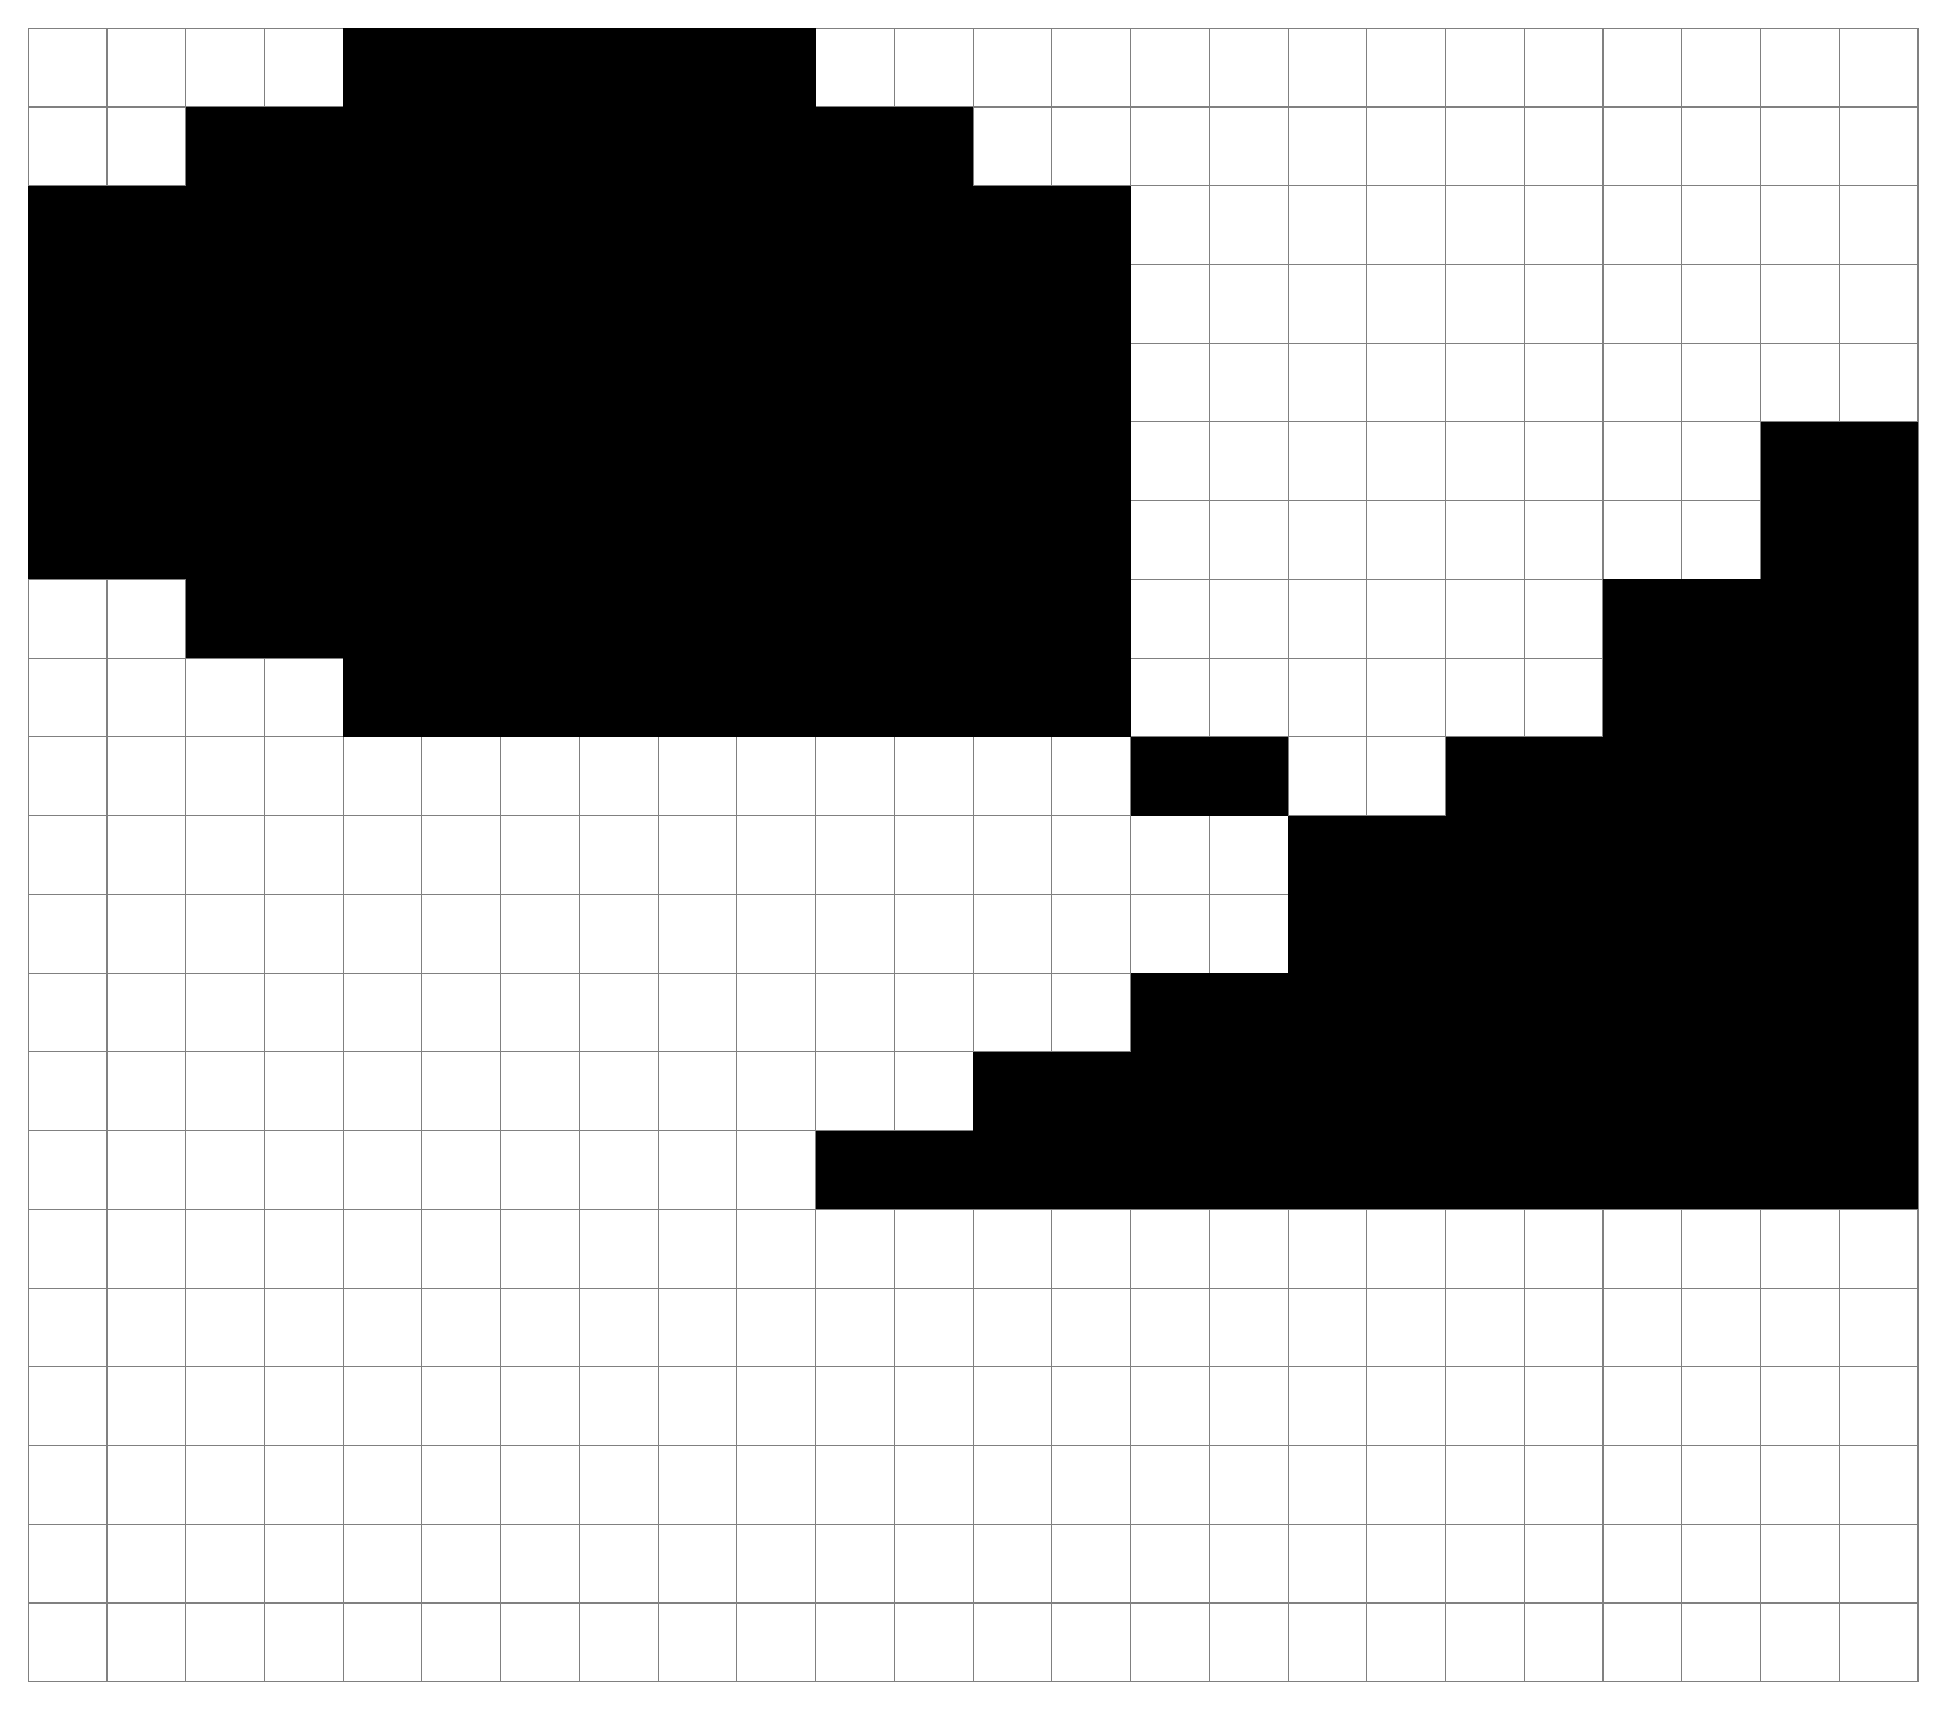
\begin{tikzpicture}

	\draw[step=1.0,gray,thin] (0,0) grid (24,21);
	\fill[\SPRITECOLOR] (4,20) rectangle ++ (1,1);
	\fill[\SPRITECOLOR] (5,20) rectangle ++ (1,1);
	\fill[\SPRITECOLOR] (6,20) rectangle ++ (1,1);
	\fill[\SPRITECOLOR] (7,20) rectangle ++ (1,1);
	\fill[\SPRITECOLOR] (8,20) rectangle ++ (1,1);
	\fill[\SPRITECOLOR] (9,20) rectangle ++ (1,1);
	\fill[\SPRITECOLOR] (2,19) rectangle ++ (1,1);
	\fill[\SPRITECOLOR] (3,19) rectangle ++ (1,1);
	\fill[\MULTICOLORTWO] (4,19) rectangle ++ (1,1);
	\fill[\MULTICOLORTWO] (5,19) rectangle ++ (1,1);
	\fill[\SPRITECOLOR] (6,19) rectangle ++ (1,1);
	\fill[\SPRITECOLOR] (7,19) rectangle ++ (1,1);
	\fill[\SPRITECOLOR] (8,19) rectangle ++ (1,1);
	\fill[\SPRITECOLOR] (9,19) rectangle ++ (1,1);
	\fill[\SPRITECOLOR] (10,19) rectangle ++ (1,1);
	\fill[\SPRITECOLOR] (11,19) rectangle ++ (1,1);
	\fill[\SPRITECOLOR] (0,18) rectangle ++ (1,1);
	\fill[\SPRITECOLOR] (1,18) rectangle ++ (1,1);
	\fill[\MULTICOLORTWO] (2,18) rectangle ++ (1,1);
	\fill[\MULTICOLORTWO] (3,18) rectangle ++ (1,1);
	\fill[\SPRITECOLOR] (4,18) rectangle ++ (1,1);
	\fill[\SPRITECOLOR] (5,18) rectangle ++ (1,1);
	\fill[\SPRITECOLOR] (6,18) rectangle ++ (1,1);
	\fill[\SPRITECOLOR] (7,18) rectangle ++ (1,1);
	\fill[\SPRITECOLOR] (8,18) rectangle ++ (1,1);
	\fill[\SPRITECOLOR] (9,18) rectangle ++ (1,1);
	\fill[\SPRITECOLOR] (10,18) rectangle ++ (1,1);
	\fill[\SPRITECOLOR] (11,18) rectangle ++ (1,1);
	\fill[\SPRITECOLOR] (12,18) rectangle ++ (1,1);
	\fill[\SPRITECOLOR] (13,18) rectangle ++ (1,1);
	\fill[\SPRITECOLOR] (0,17) rectangle ++ (1,1);
	\fill[\SPRITECOLOR] (1,17) rectangle ++ (1,1);
	\fill[\SPRITECOLOR] (2,17) rectangle ++ (1,1);
	\fill[\SPRITECOLOR] (3,17) rectangle ++ (1,1);
	\fill[\SPRITECOLOR] (4,17) rectangle ++ (1,1);
	\fill[\SPRITECOLOR] (5,17) rectangle ++ (1,1);
	\fill[\MULTICOLORONE] (6,17) rectangle ++ (1,1);
	\fill[\MULTICOLORONE] (7,17) rectangle ++ (1,1);
	\fill[\SPRITECOLOR] (8,17) rectangle ++ (1,1);
	\fill[\SPRITECOLOR] (9,17) rectangle ++ (1,1);
	\fill[\SPRITECOLOR] (10,17) rectangle ++ (1,1);
	\fill[\SPRITECOLOR] (11,17) rectangle ++ (1,1);
	\fill[\SPRITECOLOR] (12,17) rectangle ++ (1,1);
	\fill[\SPRITECOLOR] (13,17) rectangle ++ (1,1);
	\fill[\SPRITECOLOR] (0,16) rectangle ++ (1,1);
	\fill[\SPRITECOLOR] (1,16) rectangle ++ (1,1);
	\fill[\SPRITECOLOR] (2,16) rectangle ++ (1,1);
	\fill[\SPRITECOLOR] (3,16) rectangle ++ (1,1);
	\fill[\MULTICOLORONE] (4,16) rectangle ++ (1,1);
	\fill[\MULTICOLORONE] (5,16) rectangle ++ (1,1);
	\fill[\MULTICOLORONE] (6,16) rectangle ++ (1,1);
	\fill[\MULTICOLORONE] (7,16) rectangle ++ (1,1);
	\fill[\MULTICOLORONE] (8,16) rectangle ++ (1,1);
	\fill[\MULTICOLORONE] (9,16) rectangle ++ (1,1);
	\fill[\SPRITECOLOR] (10,16) rectangle ++ (1,1);
	\fill[\SPRITECOLOR] (11,16) rectangle ++ (1,1);
	\fill[\SPRITECOLOR] (12,16) rectangle ++ (1,1);
	\fill[\SPRITECOLOR] (13,16) rectangle ++ (1,1);
	\fill[\SPRITECOLOR] (0,15) rectangle ++ (1,1);
	\fill[\SPRITECOLOR] (1,15) rectangle ++ (1,1);
	\fill[\SPRITECOLOR] (2,15) rectangle ++ (1,1);
	\fill[\SPRITECOLOR] (3,15) rectangle ++ (1,1);
	\fill[\SPRITECOLOR] (4,15) rectangle ++ (1,1);
	\fill[\SPRITECOLOR] (5,15) rectangle ++ (1,1);
	\fill[\MULTICOLORONE] (6,15) rectangle ++ (1,1);
	\fill[\MULTICOLORONE] (7,15) rectangle ++ (1,1);
	\fill[\SPRITECOLOR] (8,15) rectangle ++ (1,1);
	\fill[\SPRITECOLOR] (9,15) rectangle ++ (1,1);
	\fill[\SPRITECOLOR] (10,15) rectangle ++ (1,1);
	\fill[\SPRITECOLOR] (11,15) rectangle ++ (1,1);
	\fill[\SPRITECOLOR] (12,15) rectangle ++ (1,1);
	\fill[\SPRITECOLOR] (13,15) rectangle ++ (1,1);
	\fill[\SPRITECOLOR] (22,15) rectangle ++ (1,1);
	\fill[\SPRITECOLOR] (23,15) rectangle ++ (1,1);
	\fill[\SPRITECOLOR] (0,14) rectangle ++ (1,1);
	\fill[\SPRITECOLOR] (1,14) rectangle ++ (1,1);
	\fill[\SPRITECOLOR] (2,14) rectangle ++ (1,1);
	\fill[\SPRITECOLOR] (3,14) rectangle ++ (1,1);
	\fill[\SPRITECOLOR] (4,14) rectangle ++ (1,1);
	\fill[\SPRITECOLOR] (5,14) rectangle ++ (1,1);
	\fill[\SPRITECOLOR] (6,14) rectangle ++ (1,1);
	\fill[\SPRITECOLOR] (7,14) rectangle ++ (1,1);
	\fill[\SPRITECOLOR] (8,14) rectangle ++ (1,1);
	\fill[\SPRITECOLOR] (9,14) rectangle ++ (1,1);
	\fill[\SPRITECOLOR] (10,14) rectangle ++ (1,1);
	\fill[\SPRITECOLOR] (11,14) rectangle ++ (1,1);
	\fill[\SPRITECOLOR] (12,14) rectangle ++ (1,1);
	\fill[\SPRITECOLOR] (13,14) rectangle ++ (1,1);
	\fill[\SPRITECOLOR] (22,14) rectangle ++ (1,1);
	\fill[\SPRITECOLOR] (23,14) rectangle ++ (1,1);
	\fill[\SPRITECOLOR] (2,13) rectangle ++ (1,1);
	\fill[\SPRITECOLOR] (3,13) rectangle ++ (1,1);
	\fill[\SPRITECOLOR] (4,13) rectangle ++ (1,1);
	\fill[\SPRITECOLOR] (5,13) rectangle ++ (1,1);
	\fill[\SPRITECOLOR] (6,13) rectangle ++ (1,1);
	\fill[\SPRITECOLOR] (7,13) rectangle ++ (1,1);
	\fill[\SPRITECOLOR] (8,13) rectangle ++ (1,1);
	\fill[\SPRITECOLOR] (9,13) rectangle ++ (1,1);
	\fill[\SPRITECOLOR] (10,13) rectangle ++ (1,1);
	\fill[\SPRITECOLOR] (11,13) rectangle ++ (1,1);
	\fill[\SPRITECOLOR] (12,13) rectangle ++ (1,1);
	\fill[\SPRITECOLOR] (13,13) rectangle ++ (1,1);
	\fill[\SPRITECOLOR] (20,13) rectangle ++ (1,1);
	\fill[\SPRITECOLOR] (21,13) rectangle ++ (1,1);
	\fill[\SPRITECOLOR] (22,13) rectangle ++ (1,1);
	\fill[\SPRITECOLOR] (23,13) rectangle ++ (1,1);
	\fill[\SPRITECOLOR] (4,12) rectangle ++ (1,1);
	\fill[\SPRITECOLOR] (5,12) rectangle ++ (1,1);
	\fill[\SPRITECOLOR] (6,12) rectangle ++ (1,1);
	\fill[\SPRITECOLOR] (7,12) rectangle ++ (1,1);
	\fill[\SPRITECOLOR] (8,12) rectangle ++ (1,1);
	\fill[\SPRITECOLOR] (9,12) rectangle ++ (1,1);
	\fill[\SPRITECOLOR] (10,12) rectangle ++ (1,1);
	\fill[\SPRITECOLOR] (11,12) rectangle ++ (1,1);
	\fill[\SPRITECOLOR] (12,12) rectangle ++ (1,1);
	\fill[\SPRITECOLOR] (13,12) rectangle ++ (1,1);
	\fill[\SPRITECOLOR] (20,12) rectangle ++ (1,1);
	\fill[\SPRITECOLOR] (21,12) rectangle ++ (1,1);
	\fill[\SPRITECOLOR] (22,12) rectangle ++ (1,1);
	\fill[\SPRITECOLOR] (23,12) rectangle ++ (1,1);
	\fill[\SPRITECOLOR] (14,11) rectangle ++ (1,1);
	\fill[\SPRITECOLOR] (15,11) rectangle ++ (1,1);
	\fill[\SPRITECOLOR] (18,11) rectangle ++ (1,1);
	\fill[\SPRITECOLOR] (19,11) rectangle ++ (1,1);
	\fill[\MULTICOLORONE] (20,11) rectangle ++ (1,1);
	\fill[\MULTICOLORONE] (21,11) rectangle ++ (1,1);
	\fill[\SPRITECOLOR] (22,11) rectangle ++ (1,1);
	\fill[\SPRITECOLOR] (23,11) rectangle ++ (1,1);
	\fill[\SPRITECOLOR] (16,10) rectangle ++ (1,1);
	\fill[\SPRITECOLOR] (17,10) rectangle ++ (1,1);
	\fill[\SPRITECOLOR] (18,10) rectangle ++ (1,1);
	\fill[\SPRITECOLOR] (19,10) rectangle ++ (1,1);
	\fill[\MULTICOLORONE] (20,10) rectangle ++ (1,1);
	\fill[\MULTICOLORONE] (21,10) rectangle ++ (1,1);
	\fill[\SPRITECOLOR] (22,10) rectangle ++ (1,1);
	\fill[\SPRITECOLOR] (23,10) rectangle ++ (1,1);
	\fill[\SPRITECOLOR] (16,9) rectangle ++ (1,1);
	\fill[\SPRITECOLOR] (17,9) rectangle ++ (1,1);
	\fill[\SPRITECOLOR] (18,9) rectangle ++ (1,1);
	\fill[\SPRITECOLOR] (19,9) rectangle ++ (1,1);
	\fill[\MULTICOLORONE] (20,9) rectangle ++ (1,1);
	\fill[\MULTICOLORONE] (21,9) rectangle ++ (1,1);
	\fill[\SPRITECOLOR] (22,9) rectangle ++ (1,1);
	\fill[\SPRITECOLOR] (23,9) rectangle ++ (1,1);
	\fill[\SPRITECOLOR] (14,8) rectangle ++ (1,1);
	\fill[\SPRITECOLOR] (15,8) rectangle ++ (1,1);
	\fill[\SPRITECOLOR] (16,8) rectangle ++ (1,1);
	\fill[\SPRITECOLOR] (17,8) rectangle ++ (1,1);
	\fill[\MULTICOLORONE] (18,8) rectangle ++ (1,1);
	\fill[\MULTICOLORONE] (19,8) rectangle ++ (1,1);
	\fill[\MULTICOLORONE] (20,8) rectangle ++ (1,1);
	\fill[\MULTICOLORONE] (21,8) rectangle ++ (1,1);
	\fill[\SPRITECOLOR] (22,8) rectangle ++ (1,1);
	\fill[\SPRITECOLOR] (23,8) rectangle ++ (1,1);
	\fill[\SPRITECOLOR] (12,7) rectangle ++ (1,1);
	\fill[\SPRITECOLOR] (13,7) rectangle ++ (1,1);
	\fill[\MULTICOLORONE] (14,7) rectangle ++ (1,1);
	\fill[\MULTICOLORONE] (15,7) rectangle ++ (1,1);
	\fill[\MULTICOLORONE] (16,7) rectangle ++ (1,1);
	\fill[\MULTICOLORONE] (17,7) rectangle ++ (1,1);
	\fill[\MULTICOLORONE] (18,7) rectangle ++ (1,1);
	\fill[\MULTICOLORONE] (19,7) rectangle ++ (1,1);
	\fill[\MULTICOLORONE] (20,7) rectangle ++ (1,1);
	\fill[\MULTICOLORONE] (21,7) rectangle ++ (1,1);
	\fill[\SPRITECOLOR] (22,7) rectangle ++ (1,1);
	\fill[\SPRITECOLOR] (23,7) rectangle ++ (1,1);
	\fill[\SPRITECOLOR] (10,6) rectangle ++ (1,1);
	\fill[\SPRITECOLOR] (11,6) rectangle ++ (1,1);
	\fill[\SPRITECOLOR] (12,6) rectangle ++ (1,1);
	\fill[\SPRITECOLOR] (13,6) rectangle ++ (1,1);
	\fill[\SPRITECOLOR] (14,6) rectangle ++ (1,1);
	\fill[\SPRITECOLOR] (15,6) rectangle ++ (1,1);
	\fill[\SPRITECOLOR] (16,6) rectangle ++ (1,1);
	\fill[\SPRITECOLOR] (17,6) rectangle ++ (1,1);
	\fill[\SPRITECOLOR] (18,6) rectangle ++ (1,1);
	\fill[\SPRITECOLOR] (19,6) rectangle ++ (1,1);
	\fill[\SPRITECOLOR] (20,6) rectangle ++ (1,1);
	\fill[\SPRITECOLOR] (21,6) rectangle ++ (1,1);
	\fill[\SPRITECOLOR] (22,6) rectangle ++ (1,1);
	\fill[\SPRITECOLOR] (23,6) rectangle ++ (1,1);

      \end{tikzpicture}
    \end{adjustbox}
  }\caption{UGLY\_GILBY4}
\end{figure}

	\end{subfigure}
} \\
\makecell[l]{
	\begin{subfigure}{0.3\textwidth}
    \def\MULTICOLORONE{gray}
    \def\MULTICOLORTWO{white}
    \def\SPRITECOLOR{red}
		
\begin{figure}[H]
  {
    \setlength{\tabcolsep}{3.0pt}
    \setlength\cmidrulewidth{\heavyrulewidth} % Make cmidrule = 
    \begin{adjustbox}{width=3cm,center}
      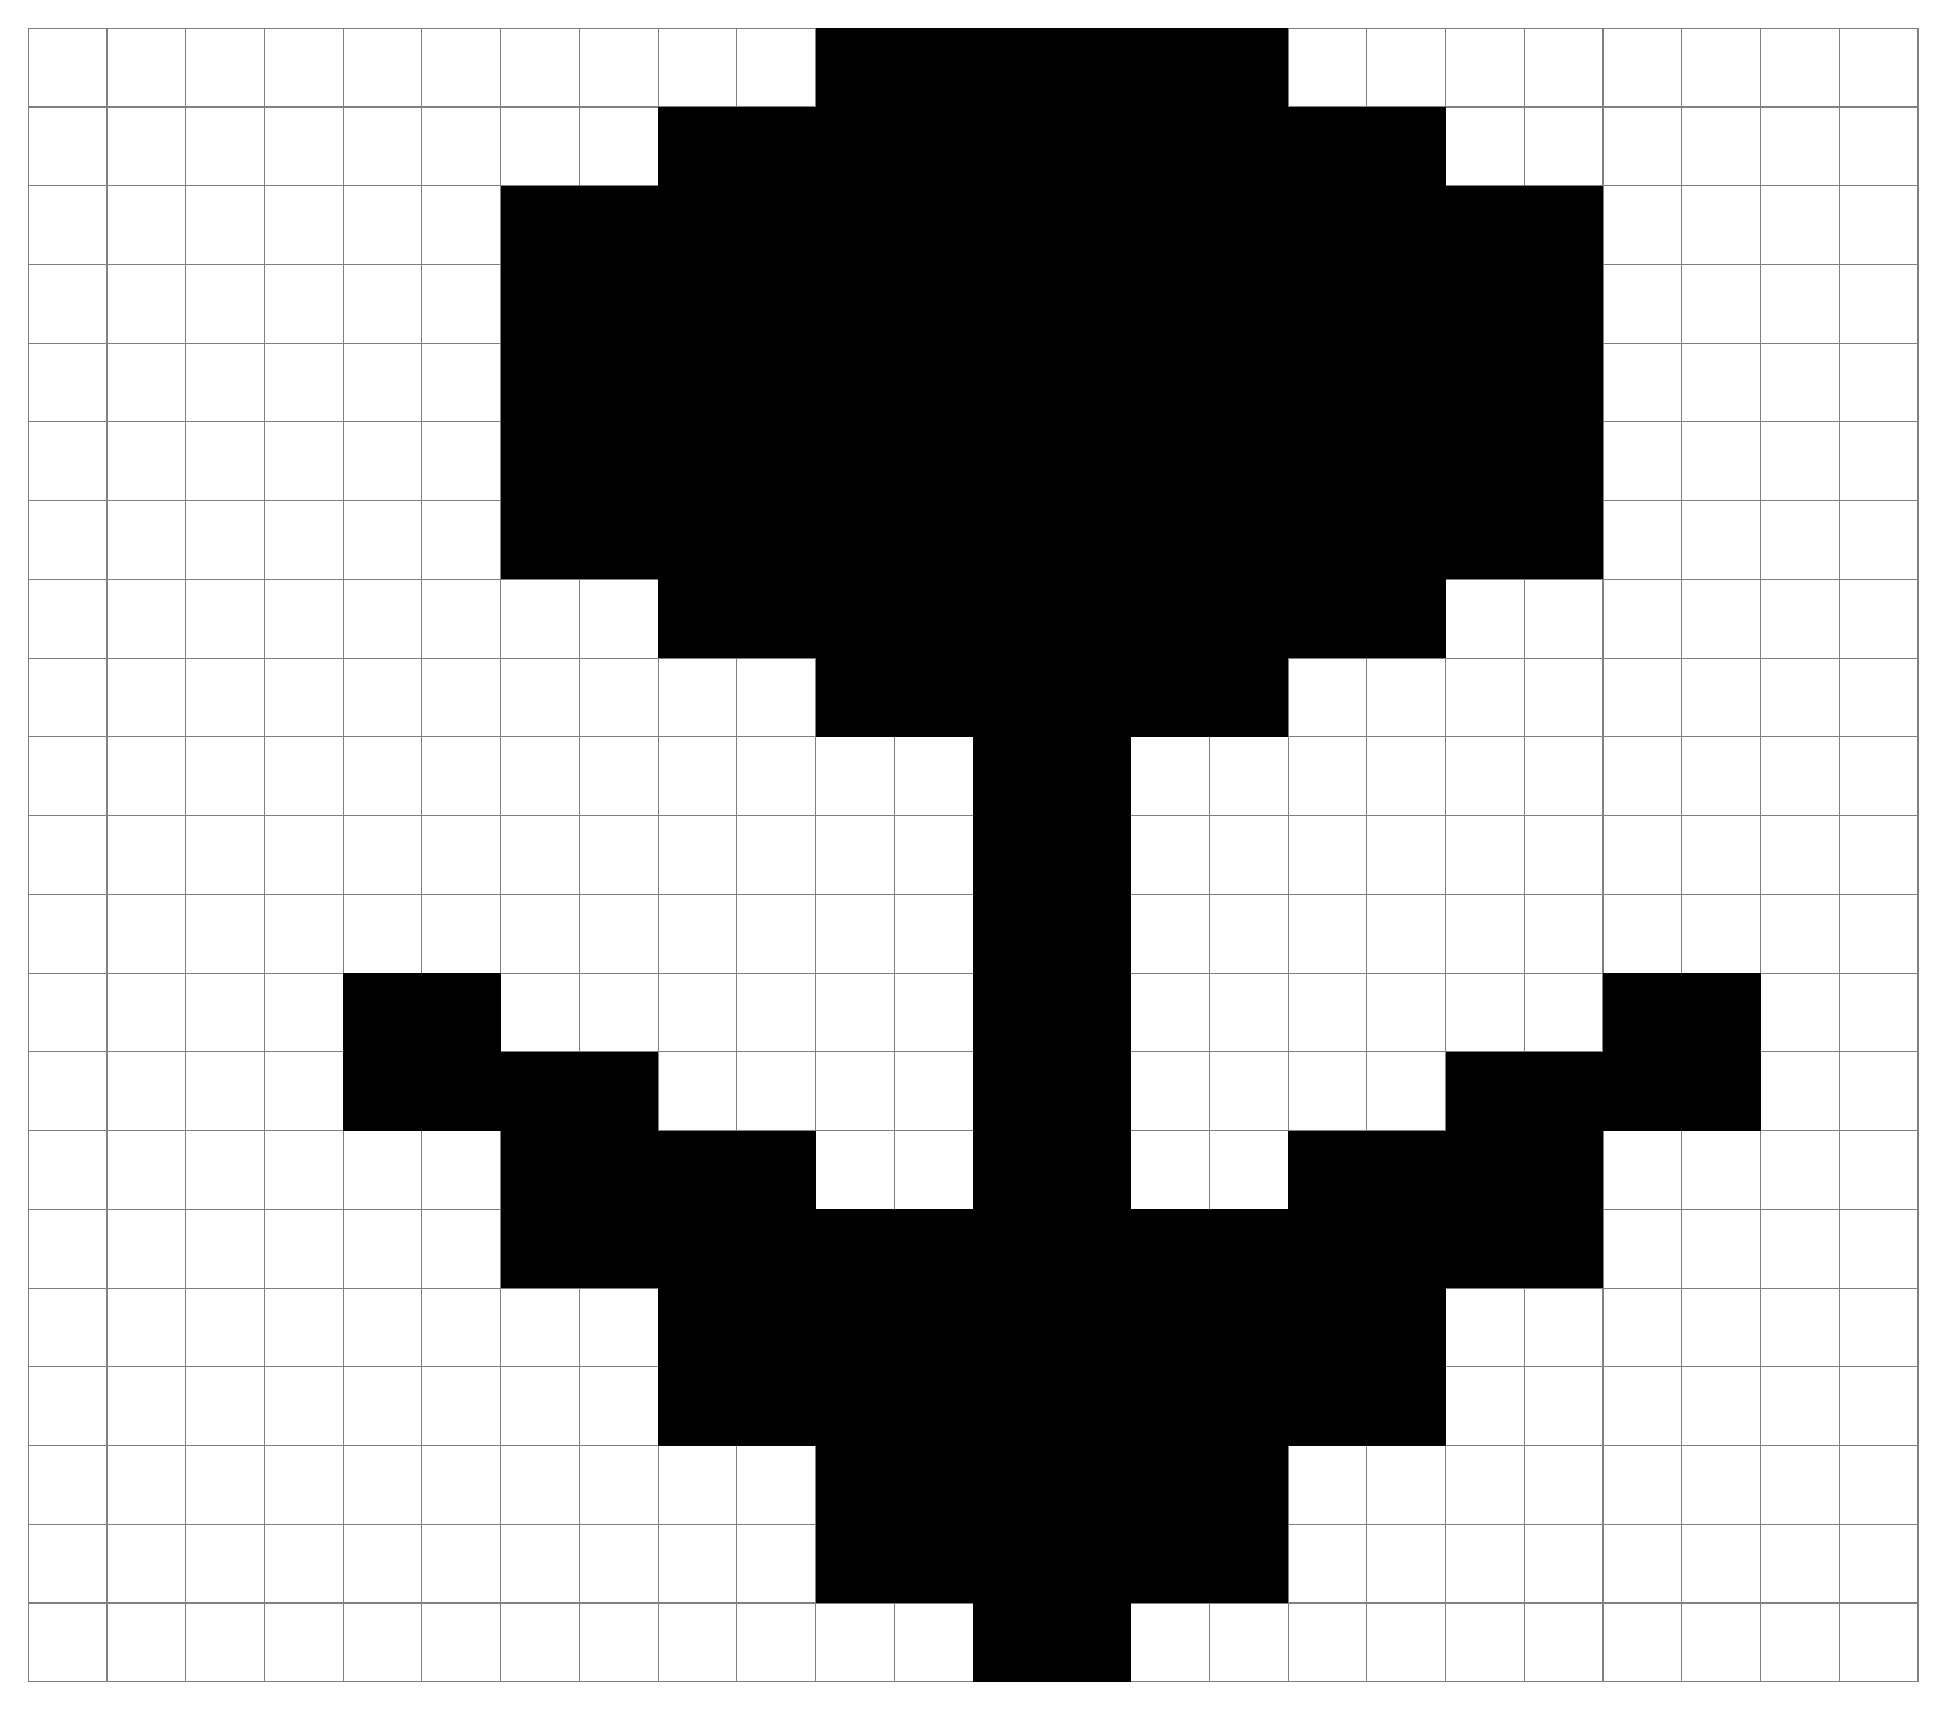
\begin{tikzpicture}

	\draw[step=1.0,gray,thin] (0,0) grid (24,21);
	\fill[\SPRITECOLOR] (10,20) rectangle ++ (1,1);
	\fill[\SPRITECOLOR] (11,20) rectangle ++ (1,1);
	\fill[\SPRITECOLOR] (12,20) rectangle ++ (1,1);
	\fill[\SPRITECOLOR] (13,20) rectangle ++ (1,1);
	\fill[\SPRITECOLOR] (14,20) rectangle ++ (1,1);
	\fill[\SPRITECOLOR] (15,20) rectangle ++ (1,1);
	\fill[\SPRITECOLOR] (8,19) rectangle ++ (1,1);
	\fill[\SPRITECOLOR] (9,19) rectangle ++ (1,1);
	\fill[\MULTICOLORTWO] (10,19) rectangle ++ (1,1);
	\fill[\MULTICOLORTWO] (11,19) rectangle ++ (1,1);
	\fill[\SPRITECOLOR] (12,19) rectangle ++ (1,1);
	\fill[\SPRITECOLOR] (13,19) rectangle ++ (1,1);
	\fill[\SPRITECOLOR] (14,19) rectangle ++ (1,1);
	\fill[\SPRITECOLOR] (15,19) rectangle ++ (1,1);
	\fill[\SPRITECOLOR] (16,19) rectangle ++ (1,1);
	\fill[\SPRITECOLOR] (17,19) rectangle ++ (1,1);
	\fill[\SPRITECOLOR] (6,18) rectangle ++ (1,1);
	\fill[\SPRITECOLOR] (7,18) rectangle ++ (1,1);
	\fill[\MULTICOLORTWO] (8,18) rectangle ++ (1,1);
	\fill[\MULTICOLORTWO] (9,18) rectangle ++ (1,1);
	\fill[\SPRITECOLOR] (10,18) rectangle ++ (1,1);
	\fill[\SPRITECOLOR] (11,18) rectangle ++ (1,1);
	\fill[\SPRITECOLOR] (12,18) rectangle ++ (1,1);
	\fill[\SPRITECOLOR] (13,18) rectangle ++ (1,1);
	\fill[\SPRITECOLOR] (14,18) rectangle ++ (1,1);
	\fill[\SPRITECOLOR] (15,18) rectangle ++ (1,1);
	\fill[\SPRITECOLOR] (16,18) rectangle ++ (1,1);
	\fill[\SPRITECOLOR] (17,18) rectangle ++ (1,1);
	\fill[\SPRITECOLOR] (18,18) rectangle ++ (1,1);
	\fill[\SPRITECOLOR] (19,18) rectangle ++ (1,1);
	\fill[\SPRITECOLOR] (6,17) rectangle ++ (1,1);
	\fill[\SPRITECOLOR] (7,17) rectangle ++ (1,1);
	\fill[\SPRITECOLOR] (8,17) rectangle ++ (1,1);
	\fill[\SPRITECOLOR] (9,17) rectangle ++ (1,1);
	\fill[\SPRITECOLOR] (10,17) rectangle ++ (1,1);
	\fill[\SPRITECOLOR] (11,17) rectangle ++ (1,1);
	\fill[\MULTICOLORONE] (12,17) rectangle ++ (1,1);
	\fill[\MULTICOLORONE] (13,17) rectangle ++ (1,1);
	\fill[\SPRITECOLOR] (14,17) rectangle ++ (1,1);
	\fill[\SPRITECOLOR] (15,17) rectangle ++ (1,1);
	\fill[\SPRITECOLOR] (16,17) rectangle ++ (1,1);
	\fill[\SPRITECOLOR] (17,17) rectangle ++ (1,1);
	\fill[\SPRITECOLOR] (18,17) rectangle ++ (1,1);
	\fill[\SPRITECOLOR] (19,17) rectangle ++ (1,1);
	\fill[\SPRITECOLOR] (6,16) rectangle ++ (1,1);
	\fill[\SPRITECOLOR] (7,16) rectangle ++ (1,1);
	\fill[\SPRITECOLOR] (8,16) rectangle ++ (1,1);
	\fill[\SPRITECOLOR] (9,16) rectangle ++ (1,1);
	\fill[\MULTICOLORONE] (10,16) rectangle ++ (1,1);
	\fill[\MULTICOLORONE] (11,16) rectangle ++ (1,1);
	\fill[\MULTICOLORONE] (12,16) rectangle ++ (1,1);
	\fill[\MULTICOLORONE] (13,16) rectangle ++ (1,1);
	\fill[\MULTICOLORONE] (14,16) rectangle ++ (1,1);
	\fill[\MULTICOLORONE] (15,16) rectangle ++ (1,1);
	\fill[\SPRITECOLOR] (16,16) rectangle ++ (1,1);
	\fill[\SPRITECOLOR] (17,16) rectangle ++ (1,1);
	\fill[\SPRITECOLOR] (18,16) rectangle ++ (1,1);
	\fill[\SPRITECOLOR] (19,16) rectangle ++ (1,1);
	\fill[\SPRITECOLOR] (6,15) rectangle ++ (1,1);
	\fill[\SPRITECOLOR] (7,15) rectangle ++ (1,1);
	\fill[\SPRITECOLOR] (8,15) rectangle ++ (1,1);
	\fill[\SPRITECOLOR] (9,15) rectangle ++ (1,1);
	\fill[\SPRITECOLOR] (10,15) rectangle ++ (1,1);
	\fill[\SPRITECOLOR] (11,15) rectangle ++ (1,1);
	\fill[\MULTICOLORONE] (12,15) rectangle ++ (1,1);
	\fill[\MULTICOLORONE] (13,15) rectangle ++ (1,1);
	\fill[\SPRITECOLOR] (14,15) rectangle ++ (1,1);
	\fill[\SPRITECOLOR] (15,15) rectangle ++ (1,1);
	\fill[\SPRITECOLOR] (16,15) rectangle ++ (1,1);
	\fill[\SPRITECOLOR] (17,15) rectangle ++ (1,1);
	\fill[\SPRITECOLOR] (18,15) rectangle ++ (1,1);
	\fill[\SPRITECOLOR] (19,15) rectangle ++ (1,1);
	\fill[\SPRITECOLOR] (6,14) rectangle ++ (1,1);
	\fill[\SPRITECOLOR] (7,14) rectangle ++ (1,1);
	\fill[\SPRITECOLOR] (8,14) rectangle ++ (1,1);
	\fill[\SPRITECOLOR] (9,14) rectangle ++ (1,1);
	\fill[\SPRITECOLOR] (10,14) rectangle ++ (1,1);
	\fill[\SPRITECOLOR] (11,14) rectangle ++ (1,1);
	\fill[\SPRITECOLOR] (12,14) rectangle ++ (1,1);
	\fill[\SPRITECOLOR] (13,14) rectangle ++ (1,1);
	\fill[\SPRITECOLOR] (14,14) rectangle ++ (1,1);
	\fill[\SPRITECOLOR] (15,14) rectangle ++ (1,1);
	\fill[\SPRITECOLOR] (16,14) rectangle ++ (1,1);
	\fill[\SPRITECOLOR] (17,14) rectangle ++ (1,1);
	\fill[\SPRITECOLOR] (18,14) rectangle ++ (1,1);
	\fill[\SPRITECOLOR] (19,14) rectangle ++ (1,1);
	\fill[\SPRITECOLOR] (8,13) rectangle ++ (1,1);
	\fill[\SPRITECOLOR] (9,13) rectangle ++ (1,1);
	\fill[\SPRITECOLOR] (10,13) rectangle ++ (1,1);
	\fill[\SPRITECOLOR] (11,13) rectangle ++ (1,1);
	\fill[\SPRITECOLOR] (12,13) rectangle ++ (1,1);
	\fill[\SPRITECOLOR] (13,13) rectangle ++ (1,1);
	\fill[\SPRITECOLOR] (14,13) rectangle ++ (1,1);
	\fill[\SPRITECOLOR] (15,13) rectangle ++ (1,1);
	\fill[\SPRITECOLOR] (16,13) rectangle ++ (1,1);
	\fill[\SPRITECOLOR] (17,13) rectangle ++ (1,1);
	\fill[\SPRITECOLOR] (10,12) rectangle ++ (1,1);
	\fill[\SPRITECOLOR] (11,12) rectangle ++ (1,1);
	\fill[\SPRITECOLOR] (12,12) rectangle ++ (1,1);
	\fill[\SPRITECOLOR] (13,12) rectangle ++ (1,1);
	\fill[\SPRITECOLOR] (14,12) rectangle ++ (1,1);
	\fill[\SPRITECOLOR] (15,12) rectangle ++ (1,1);
	\fill[\SPRITECOLOR] (12,11) rectangle ++ (1,1);
	\fill[\SPRITECOLOR] (13,11) rectangle ++ (1,1);
	\fill[\SPRITECOLOR] (12,10) rectangle ++ (1,1);
	\fill[\SPRITECOLOR] (13,10) rectangle ++ (1,1);
	\fill[\SPRITECOLOR] (12,9) rectangle ++ (1,1);
	\fill[\SPRITECOLOR] (13,9) rectangle ++ (1,1);
	\fill[\SPRITECOLOR] (4,8) rectangle ++ (1,1);
	\fill[\SPRITECOLOR] (5,8) rectangle ++ (1,1);
	\fill[\SPRITECOLOR] (12,8) rectangle ++ (1,1);
	\fill[\SPRITECOLOR] (13,8) rectangle ++ (1,1);
	\fill[\SPRITECOLOR] (20,8) rectangle ++ (1,1);
	\fill[\SPRITECOLOR] (21,8) rectangle ++ (1,1);
	\fill[\SPRITECOLOR] (4,7) rectangle ++ (1,1);
	\fill[\SPRITECOLOR] (5,7) rectangle ++ (1,1);
	\fill[\SPRITECOLOR] (6,7) rectangle ++ (1,1);
	\fill[\SPRITECOLOR] (7,7) rectangle ++ (1,1);
	\fill[\SPRITECOLOR] (12,7) rectangle ++ (1,1);
	\fill[\SPRITECOLOR] (13,7) rectangle ++ (1,1);
	\fill[\SPRITECOLOR] (18,7) rectangle ++ (1,1);
	\fill[\SPRITECOLOR] (19,7) rectangle ++ (1,1);
	\fill[\SPRITECOLOR] (20,7) rectangle ++ (1,1);
	\fill[\SPRITECOLOR] (21,7) rectangle ++ (1,1);
	\fill[\MULTICOLORONE] (6,6) rectangle ++ (1,1);
	\fill[\MULTICOLORONE] (7,6) rectangle ++ (1,1);
	\fill[\SPRITECOLOR] (8,6) rectangle ++ (1,1);
	\fill[\SPRITECOLOR] (9,6) rectangle ++ (1,1);
	\fill[\SPRITECOLOR] (12,6) rectangle ++ (1,1);
	\fill[\SPRITECOLOR] (13,6) rectangle ++ (1,1);
	\fill[\SPRITECOLOR] (16,6) rectangle ++ (1,1);
	\fill[\SPRITECOLOR] (17,6) rectangle ++ (1,1);
	\fill[\MULTICOLORONE] (18,6) rectangle ++ (1,1);
	\fill[\MULTICOLORONE] (19,6) rectangle ++ (1,1);
	\fill[\SPRITECOLOR] (6,5) rectangle ++ (1,1);
	\fill[\SPRITECOLOR] (7,5) rectangle ++ (1,1);
	\fill[\MULTICOLORONE] (8,5) rectangle ++ (1,1);
	\fill[\MULTICOLORONE] (9,5) rectangle ++ (1,1);
	\fill[\SPRITECOLOR] (10,5) rectangle ++ (1,1);
	\fill[\SPRITECOLOR] (11,5) rectangle ++ (1,1);
	\fill[\SPRITECOLOR] (12,5) rectangle ++ (1,1);
	\fill[\SPRITECOLOR] (13,5) rectangle ++ (1,1);
	\fill[\SPRITECOLOR] (14,5) rectangle ++ (1,1);
	\fill[\SPRITECOLOR] (15,5) rectangle ++ (1,1);
	\fill[\MULTICOLORONE] (16,5) rectangle ++ (1,1);
	\fill[\MULTICOLORONE] (17,5) rectangle ++ (1,1);
	\fill[\SPRITECOLOR] (18,5) rectangle ++ (1,1);
	\fill[\SPRITECOLOR] (19,5) rectangle ++ (1,1);
	\fill[\SPRITECOLOR] (8,4) rectangle ++ (1,1);
	\fill[\SPRITECOLOR] (9,4) rectangle ++ (1,1);
	\fill[\MULTICOLORONE] (10,4) rectangle ++ (1,1);
	\fill[\MULTICOLORONE] (11,4) rectangle ++ (1,1);
	\fill[\MULTICOLORONE] (12,4) rectangle ++ (1,1);
	\fill[\MULTICOLORONE] (13,4) rectangle ++ (1,1);
	\fill[\MULTICOLORONE] (14,4) rectangle ++ (1,1);
	\fill[\MULTICOLORONE] (15,4) rectangle ++ (1,1);
	\fill[\SPRITECOLOR] (16,4) rectangle ++ (1,1);
	\fill[\SPRITECOLOR] (17,4) rectangle ++ (1,1);
	\fill[\SPRITECOLOR] (8,3) rectangle ++ (1,1);
	\fill[\SPRITECOLOR] (9,3) rectangle ++ (1,1);
	\fill[\MULTICOLORONE] (10,3) rectangle ++ (1,1);
	\fill[\MULTICOLORONE] (11,3) rectangle ++ (1,1);
	\fill[\MULTICOLORONE] (12,3) rectangle ++ (1,1);
	\fill[\MULTICOLORONE] (13,3) rectangle ++ (1,1);
	\fill[\MULTICOLORONE] (14,3) rectangle ++ (1,1);
	\fill[\MULTICOLORONE] (15,3) rectangle ++ (1,1);
	\fill[\SPRITECOLOR] (16,3) rectangle ++ (1,1);
	\fill[\SPRITECOLOR] (17,3) rectangle ++ (1,1);
	\fill[\SPRITECOLOR] (10,2) rectangle ++ (1,1);
	\fill[\SPRITECOLOR] (11,2) rectangle ++ (1,1);
	\fill[\MULTICOLORONE] (12,2) rectangle ++ (1,1);
	\fill[\MULTICOLORONE] (13,2) rectangle ++ (1,1);
	\fill[\SPRITECOLOR] (14,2) rectangle ++ (1,1);
	\fill[\SPRITECOLOR] (15,2) rectangle ++ (1,1);
	\fill[\SPRITECOLOR] (10,1) rectangle ++ (1,1);
	\fill[\SPRITECOLOR] (11,1) rectangle ++ (1,1);
	\fill[\SPRITECOLOR] (12,1) rectangle ++ (1,1);
	\fill[\SPRITECOLOR] (13,1) rectangle ++ (1,1);
	\fill[\SPRITECOLOR] (14,1) rectangle ++ (1,1);
	\fill[\SPRITECOLOR] (15,1) rectangle ++ (1,1);
	\fill[\SPRITECOLOR] (12,0) rectangle ++ (1,1);
	\fill[\SPRITECOLOR] (13,0) rectangle ++ (1,1);

      \end{tikzpicture}
    \end{adjustbox}
  }\caption{UGLY\_GILBY5}
\end{figure}

	\end{subfigure}
} & 
\makecell[l]{
	\begin{subfigure}{0.3\textwidth}
    \def\MULTICOLORONE{gray}
    \def\MULTICOLORTWO{white}
    \def\SPRITECOLOR{red}
		
\begin{figure}[H]
  {
    \setlength{\tabcolsep}{3.0pt}
    \setlength\cmidrulewidth{\heavyrulewidth} % Make cmidrule = 
    \begin{adjustbox}{width=3cm,center}
      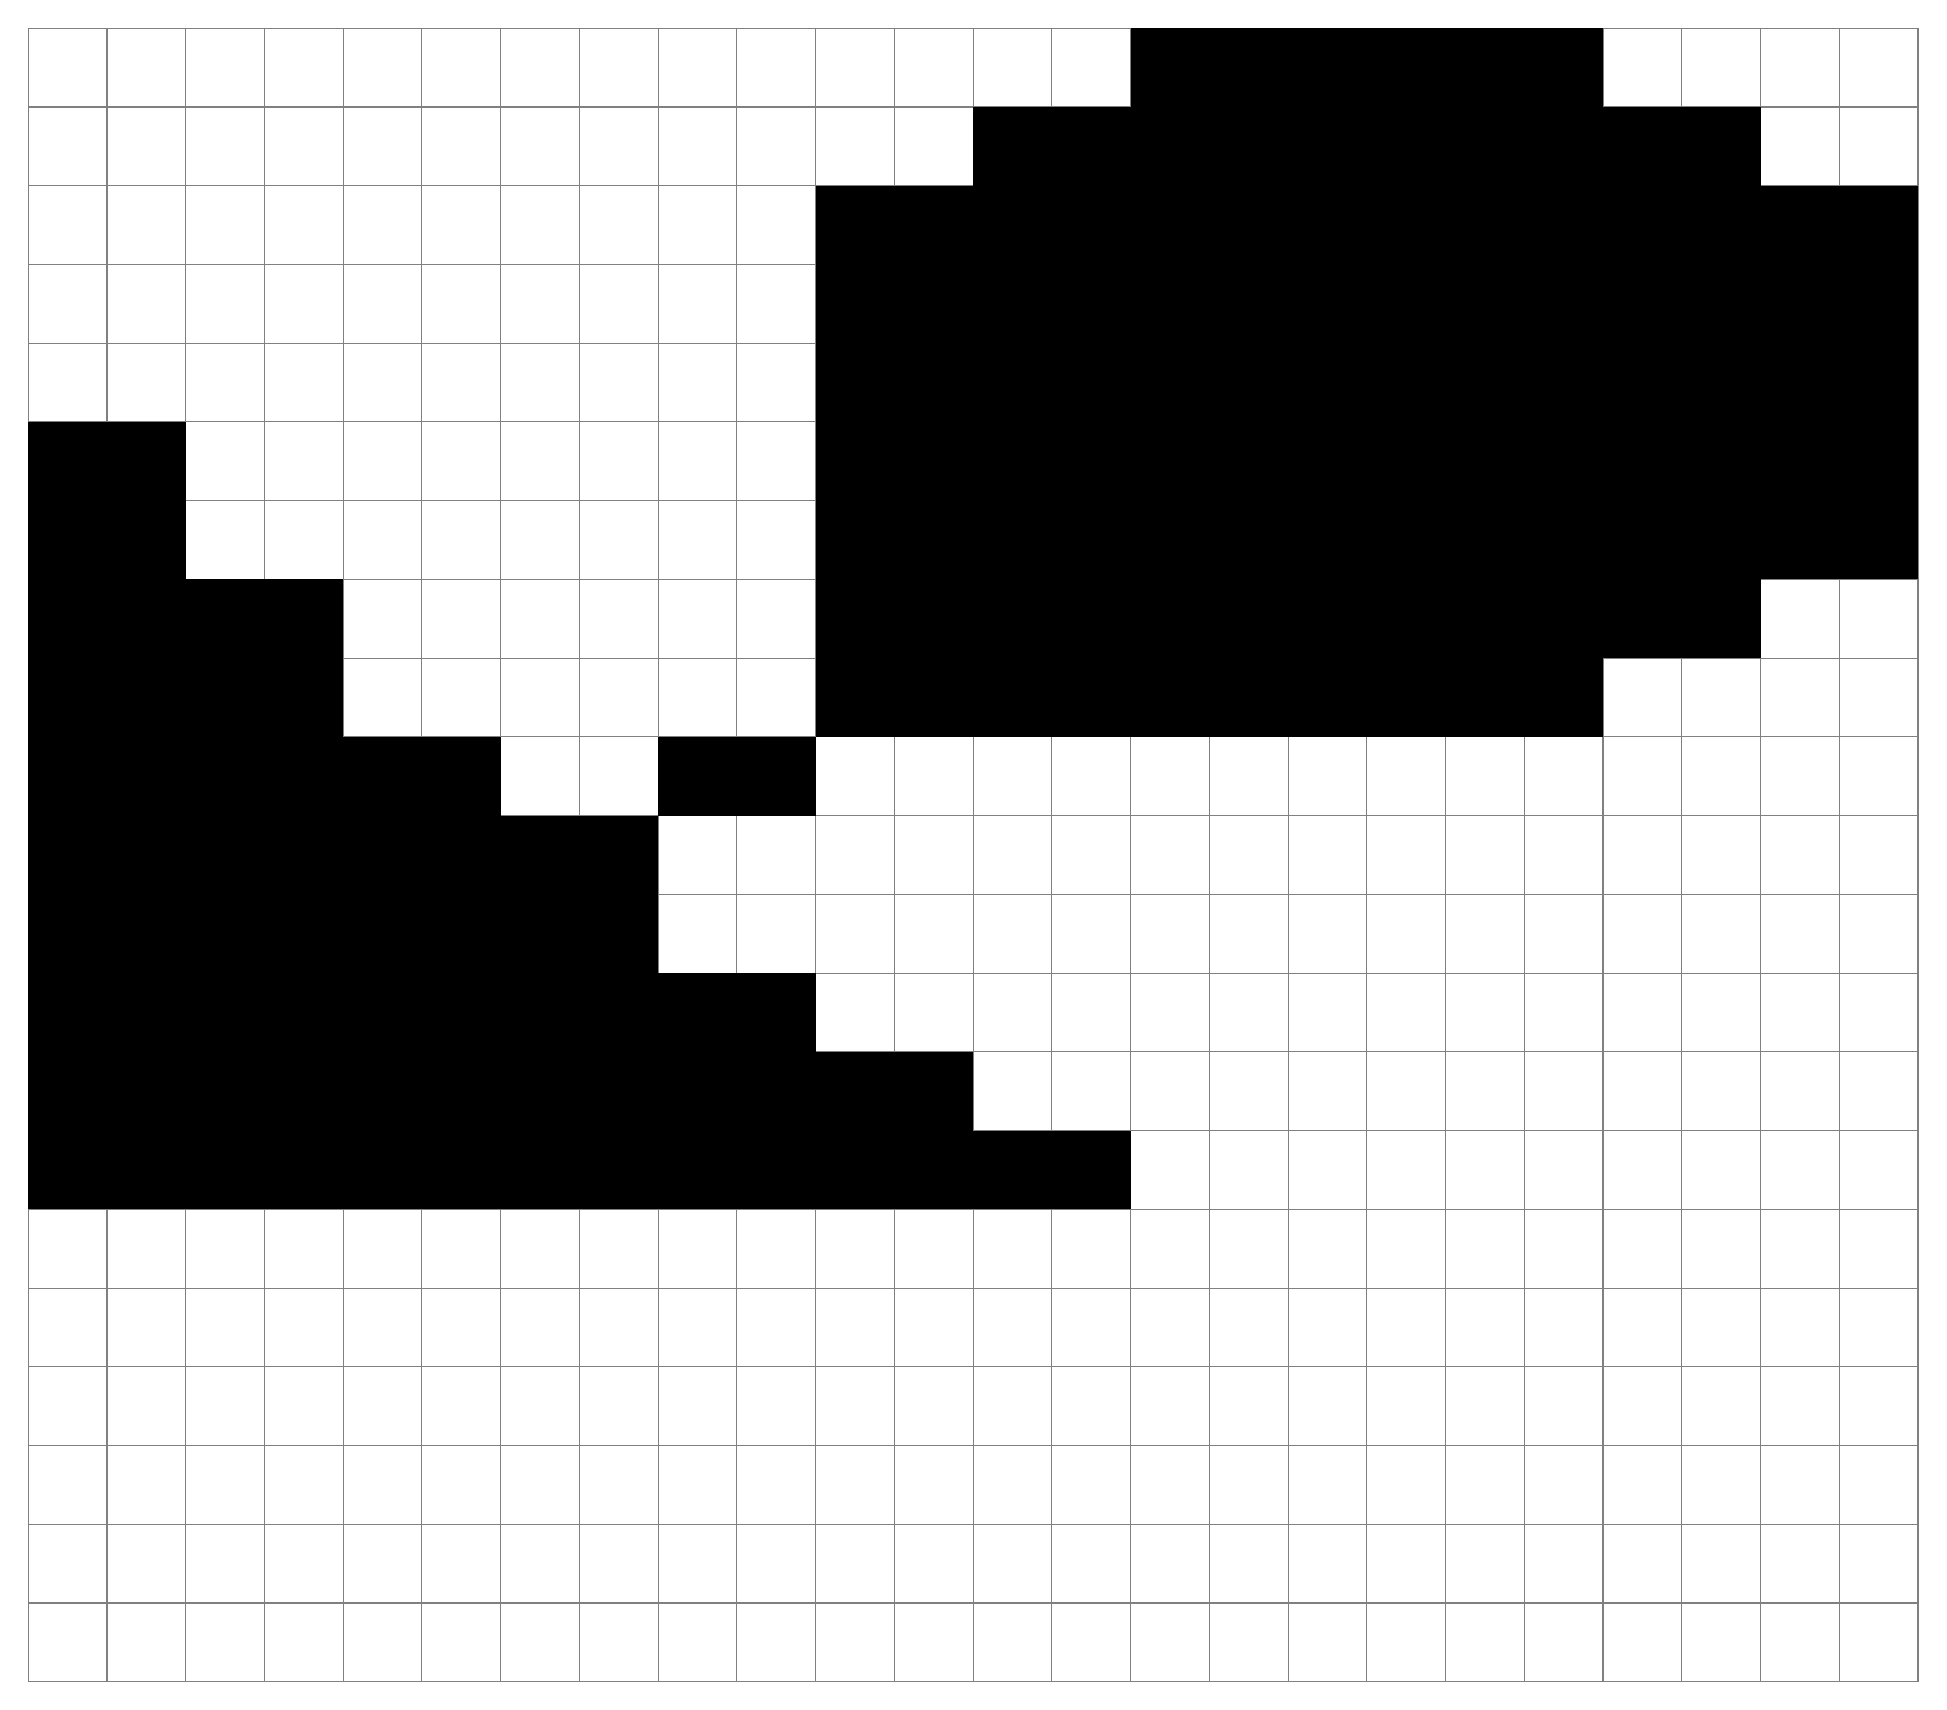
\begin{tikzpicture}

	\draw[step=1.0,gray,thin] (0,0) grid (24,21);
	\fill[\SPRITECOLOR] (14,20) rectangle ++ (1,1);
	\fill[\SPRITECOLOR] (15,20) rectangle ++ (1,1);
	\fill[\SPRITECOLOR] (16,20) rectangle ++ (1,1);
	\fill[\SPRITECOLOR] (17,20) rectangle ++ (1,1);
	\fill[\SPRITECOLOR] (18,20) rectangle ++ (1,1);
	\fill[\SPRITECOLOR] (19,20) rectangle ++ (1,1);
	\fill[\SPRITECOLOR] (12,19) rectangle ++ (1,1);
	\fill[\SPRITECOLOR] (13,19) rectangle ++ (1,1);
	\fill[\MULTICOLORTWO] (14,19) rectangle ++ (1,1);
	\fill[\MULTICOLORTWO] (15,19) rectangle ++ (1,1);
	\fill[\SPRITECOLOR] (16,19) rectangle ++ (1,1);
	\fill[\SPRITECOLOR] (17,19) rectangle ++ (1,1);
	\fill[\SPRITECOLOR] (18,19) rectangle ++ (1,1);
	\fill[\SPRITECOLOR] (19,19) rectangle ++ (1,1);
	\fill[\SPRITECOLOR] (20,19) rectangle ++ (1,1);
	\fill[\SPRITECOLOR] (21,19) rectangle ++ (1,1);
	\fill[\SPRITECOLOR] (10,18) rectangle ++ (1,1);
	\fill[\SPRITECOLOR] (11,18) rectangle ++ (1,1);
	\fill[\MULTICOLORTWO] (12,18) rectangle ++ (1,1);
	\fill[\MULTICOLORTWO] (13,18) rectangle ++ (1,1);
	\fill[\SPRITECOLOR] (14,18) rectangle ++ (1,1);
	\fill[\SPRITECOLOR] (15,18) rectangle ++ (1,1);
	\fill[\SPRITECOLOR] (16,18) rectangle ++ (1,1);
	\fill[\SPRITECOLOR] (17,18) rectangle ++ (1,1);
	\fill[\SPRITECOLOR] (18,18) rectangle ++ (1,1);
	\fill[\SPRITECOLOR] (19,18) rectangle ++ (1,1);
	\fill[\SPRITECOLOR] (20,18) rectangle ++ (1,1);
	\fill[\SPRITECOLOR] (21,18) rectangle ++ (1,1);
	\fill[\SPRITECOLOR] (22,18) rectangle ++ (1,1);
	\fill[\SPRITECOLOR] (23,18) rectangle ++ (1,1);
	\fill[\SPRITECOLOR] (10,17) rectangle ++ (1,1);
	\fill[\SPRITECOLOR] (11,17) rectangle ++ (1,1);
	\fill[\SPRITECOLOR] (12,17) rectangle ++ (1,1);
	\fill[\SPRITECOLOR] (13,17) rectangle ++ (1,1);
	\fill[\SPRITECOLOR] (14,17) rectangle ++ (1,1);
	\fill[\SPRITECOLOR] (15,17) rectangle ++ (1,1);
	\fill[\MULTICOLORONE] (16,17) rectangle ++ (1,1);
	\fill[\MULTICOLORONE] (17,17) rectangle ++ (1,1);
	\fill[\SPRITECOLOR] (18,17) rectangle ++ (1,1);
	\fill[\SPRITECOLOR] (19,17) rectangle ++ (1,1);
	\fill[\SPRITECOLOR] (20,17) rectangle ++ (1,1);
	\fill[\SPRITECOLOR] (21,17) rectangle ++ (1,1);
	\fill[\SPRITECOLOR] (22,17) rectangle ++ (1,1);
	\fill[\SPRITECOLOR] (23,17) rectangle ++ (1,1);
	\fill[\SPRITECOLOR] (10,16) rectangle ++ (1,1);
	\fill[\SPRITECOLOR] (11,16) rectangle ++ (1,1);
	\fill[\SPRITECOLOR] (12,16) rectangle ++ (1,1);
	\fill[\SPRITECOLOR] (13,16) rectangle ++ (1,1);
	\fill[\MULTICOLORONE] (14,16) rectangle ++ (1,1);
	\fill[\MULTICOLORONE] (15,16) rectangle ++ (1,1);
	\fill[\MULTICOLORONE] (16,16) rectangle ++ (1,1);
	\fill[\MULTICOLORONE] (17,16) rectangle ++ (1,1);
	\fill[\MULTICOLORONE] (18,16) rectangle ++ (1,1);
	\fill[\MULTICOLORONE] (19,16) rectangle ++ (1,1);
	\fill[\SPRITECOLOR] (20,16) rectangle ++ (1,1);
	\fill[\SPRITECOLOR] (21,16) rectangle ++ (1,1);
	\fill[\SPRITECOLOR] (22,16) rectangle ++ (1,1);
	\fill[\SPRITECOLOR] (23,16) rectangle ++ (1,1);
	\fill[\SPRITECOLOR] (0,15) rectangle ++ (1,1);
	\fill[\SPRITECOLOR] (1,15) rectangle ++ (1,1);
	\fill[\SPRITECOLOR] (10,15) rectangle ++ (1,1);
	\fill[\SPRITECOLOR] (11,15) rectangle ++ (1,1);
	\fill[\SPRITECOLOR] (12,15) rectangle ++ (1,1);
	\fill[\SPRITECOLOR] (13,15) rectangle ++ (1,1);
	\fill[\SPRITECOLOR] (14,15) rectangle ++ (1,1);
	\fill[\SPRITECOLOR] (15,15) rectangle ++ (1,1);
	\fill[\MULTICOLORONE] (16,15) rectangle ++ (1,1);
	\fill[\MULTICOLORONE] (17,15) rectangle ++ (1,1);
	\fill[\SPRITECOLOR] (18,15) rectangle ++ (1,1);
	\fill[\SPRITECOLOR] (19,15) rectangle ++ (1,1);
	\fill[\SPRITECOLOR] (20,15) rectangle ++ (1,1);
	\fill[\SPRITECOLOR] (21,15) rectangle ++ (1,1);
	\fill[\SPRITECOLOR] (22,15) rectangle ++ (1,1);
	\fill[\SPRITECOLOR] (23,15) rectangle ++ (1,1);
	\fill[\SPRITECOLOR] (0,14) rectangle ++ (1,1);
	\fill[\SPRITECOLOR] (1,14) rectangle ++ (1,1);
	\fill[\SPRITECOLOR] (10,14) rectangle ++ (1,1);
	\fill[\SPRITECOLOR] (11,14) rectangle ++ (1,1);
	\fill[\SPRITECOLOR] (12,14) rectangle ++ (1,1);
	\fill[\SPRITECOLOR] (13,14) rectangle ++ (1,1);
	\fill[\SPRITECOLOR] (14,14) rectangle ++ (1,1);
	\fill[\SPRITECOLOR] (15,14) rectangle ++ (1,1);
	\fill[\SPRITECOLOR] (16,14) rectangle ++ (1,1);
	\fill[\SPRITECOLOR] (17,14) rectangle ++ (1,1);
	\fill[\SPRITECOLOR] (18,14) rectangle ++ (1,1);
	\fill[\SPRITECOLOR] (19,14) rectangle ++ (1,1);
	\fill[\SPRITECOLOR] (20,14) rectangle ++ (1,1);
	\fill[\SPRITECOLOR] (21,14) rectangle ++ (1,1);
	\fill[\SPRITECOLOR] (22,14) rectangle ++ (1,1);
	\fill[\SPRITECOLOR] (23,14) rectangle ++ (1,1);
	\fill[\SPRITECOLOR] (0,13) rectangle ++ (1,1);
	\fill[\SPRITECOLOR] (1,13) rectangle ++ (1,1);
	\fill[\SPRITECOLOR] (2,13) rectangle ++ (1,1);
	\fill[\SPRITECOLOR] (3,13) rectangle ++ (1,1);
	\fill[\SPRITECOLOR] (10,13) rectangle ++ (1,1);
	\fill[\SPRITECOLOR] (11,13) rectangle ++ (1,1);
	\fill[\SPRITECOLOR] (12,13) rectangle ++ (1,1);
	\fill[\SPRITECOLOR] (13,13) rectangle ++ (1,1);
	\fill[\SPRITECOLOR] (14,13) rectangle ++ (1,1);
	\fill[\SPRITECOLOR] (15,13) rectangle ++ (1,1);
	\fill[\SPRITECOLOR] (16,13) rectangle ++ (1,1);
	\fill[\SPRITECOLOR] (17,13) rectangle ++ (1,1);
	\fill[\SPRITECOLOR] (18,13) rectangle ++ (1,1);
	\fill[\SPRITECOLOR] (19,13) rectangle ++ (1,1);
	\fill[\SPRITECOLOR] (20,13) rectangle ++ (1,1);
	\fill[\SPRITECOLOR] (21,13) rectangle ++ (1,1);
	\fill[\SPRITECOLOR] (0,12) rectangle ++ (1,1);
	\fill[\SPRITECOLOR] (1,12) rectangle ++ (1,1);
	\fill[\SPRITECOLOR] (2,12) rectangle ++ (1,1);
	\fill[\SPRITECOLOR] (3,12) rectangle ++ (1,1);
	\fill[\SPRITECOLOR] (10,12) rectangle ++ (1,1);
	\fill[\SPRITECOLOR] (11,12) rectangle ++ (1,1);
	\fill[\SPRITECOLOR] (12,12) rectangle ++ (1,1);
	\fill[\SPRITECOLOR] (13,12) rectangle ++ (1,1);
	\fill[\SPRITECOLOR] (14,12) rectangle ++ (1,1);
	\fill[\SPRITECOLOR] (15,12) rectangle ++ (1,1);
	\fill[\SPRITECOLOR] (16,12) rectangle ++ (1,1);
	\fill[\SPRITECOLOR] (17,12) rectangle ++ (1,1);
	\fill[\SPRITECOLOR] (18,12) rectangle ++ (1,1);
	\fill[\SPRITECOLOR] (19,12) rectangle ++ (1,1);
	\fill[\SPRITECOLOR] (0,11) rectangle ++ (1,1);
	\fill[\SPRITECOLOR] (1,11) rectangle ++ (1,1);
	\fill[\MULTICOLORONE] (2,11) rectangle ++ (1,1);
	\fill[\MULTICOLORONE] (3,11) rectangle ++ (1,1);
	\fill[\SPRITECOLOR] (4,11) rectangle ++ (1,1);
	\fill[\SPRITECOLOR] (5,11) rectangle ++ (1,1);
	\fill[\SPRITECOLOR] (8,11) rectangle ++ (1,1);
	\fill[\SPRITECOLOR] (9,11) rectangle ++ (1,1);
	\fill[\SPRITECOLOR] (0,10) rectangle ++ (1,1);
	\fill[\SPRITECOLOR] (1,10) rectangle ++ (1,1);
	\fill[\MULTICOLORONE] (2,10) rectangle ++ (1,1);
	\fill[\MULTICOLORONE] (3,10) rectangle ++ (1,1);
	\fill[\SPRITECOLOR] (4,10) rectangle ++ (1,1);
	\fill[\SPRITECOLOR] (5,10) rectangle ++ (1,1);
	\fill[\SPRITECOLOR] (6,10) rectangle ++ (1,1);
	\fill[\SPRITECOLOR] (7,10) rectangle ++ (1,1);
	\fill[\SPRITECOLOR] (0,9) rectangle ++ (1,1);
	\fill[\SPRITECOLOR] (1,9) rectangle ++ (1,1);
	\fill[\MULTICOLORONE] (2,9) rectangle ++ (1,1);
	\fill[\MULTICOLORONE] (3,9) rectangle ++ (1,1);
	\fill[\SPRITECOLOR] (4,9) rectangle ++ (1,1);
	\fill[\SPRITECOLOR] (5,9) rectangle ++ (1,1);
	\fill[\SPRITECOLOR] (6,9) rectangle ++ (1,1);
	\fill[\SPRITECOLOR] (7,9) rectangle ++ (1,1);
	\fill[\SPRITECOLOR] (0,8) rectangle ++ (1,1);
	\fill[\SPRITECOLOR] (1,8) rectangle ++ (1,1);
	\fill[\MULTICOLORONE] (2,8) rectangle ++ (1,1);
	\fill[\MULTICOLORONE] (3,8) rectangle ++ (1,1);
	\fill[\MULTICOLORONE] (4,8) rectangle ++ (1,1);
	\fill[\MULTICOLORONE] (5,8) rectangle ++ (1,1);
	\fill[\SPRITECOLOR] (6,8) rectangle ++ (1,1);
	\fill[\SPRITECOLOR] (7,8) rectangle ++ (1,1);
	\fill[\SPRITECOLOR] (8,8) rectangle ++ (1,1);
	\fill[\SPRITECOLOR] (9,8) rectangle ++ (1,1);
	\fill[\SPRITECOLOR] (0,7) rectangle ++ (1,1);
	\fill[\SPRITECOLOR] (1,7) rectangle ++ (1,1);
	\fill[\MULTICOLORONE] (2,7) rectangle ++ (1,1);
	\fill[\MULTICOLORONE] (3,7) rectangle ++ (1,1);
	\fill[\MULTICOLORONE] (4,7) rectangle ++ (1,1);
	\fill[\MULTICOLORONE] (5,7) rectangle ++ (1,1);
	\fill[\MULTICOLORONE] (6,7) rectangle ++ (1,1);
	\fill[\MULTICOLORONE] (7,7) rectangle ++ (1,1);
	\fill[\MULTICOLORONE] (8,7) rectangle ++ (1,1);
	\fill[\MULTICOLORONE] (9,7) rectangle ++ (1,1);
	\fill[\SPRITECOLOR] (10,7) rectangle ++ (1,1);
	\fill[\SPRITECOLOR] (11,7) rectangle ++ (1,1);
	\fill[\SPRITECOLOR] (0,6) rectangle ++ (1,1);
	\fill[\SPRITECOLOR] (1,6) rectangle ++ (1,1);
	\fill[\SPRITECOLOR] (2,6) rectangle ++ (1,1);
	\fill[\SPRITECOLOR] (3,6) rectangle ++ (1,1);
	\fill[\SPRITECOLOR] (4,6) rectangle ++ (1,1);
	\fill[\SPRITECOLOR] (5,6) rectangle ++ (1,1);
	\fill[\SPRITECOLOR] (6,6) rectangle ++ (1,1);
	\fill[\SPRITECOLOR] (7,6) rectangle ++ (1,1);
	\fill[\SPRITECOLOR] (8,6) rectangle ++ (1,1);
	\fill[\SPRITECOLOR] (9,6) rectangle ++ (1,1);
	\fill[\SPRITECOLOR] (10,6) rectangle ++ (1,1);
	\fill[\SPRITECOLOR] (11,6) rectangle ++ (1,1);
	\fill[\SPRITECOLOR] (12,6) rectangle ++ (1,1);
	\fill[\SPRITECOLOR] (13,6) rectangle ++ (1,1);

      \end{tikzpicture}
    \end{adjustbox}
  }\caption{UGLY\_GILBY6}
\end{figure}

	\end{subfigure}
} & 
\makecell[l]{
	\begin{subfigure}{0.3\textwidth}
    \def\MULTICOLORONE{gray}
    \def\MULTICOLORTWO{white}
    \def\SPRITECOLOR{red}
		
\begin{figure}[H]
  {
    \setlength{\tabcolsep}{3.0pt}
    \setlength\cmidrulewidth{\heavyrulewidth} % Make cmidrule = 
    \begin{adjustbox}{width=3cm,center}
      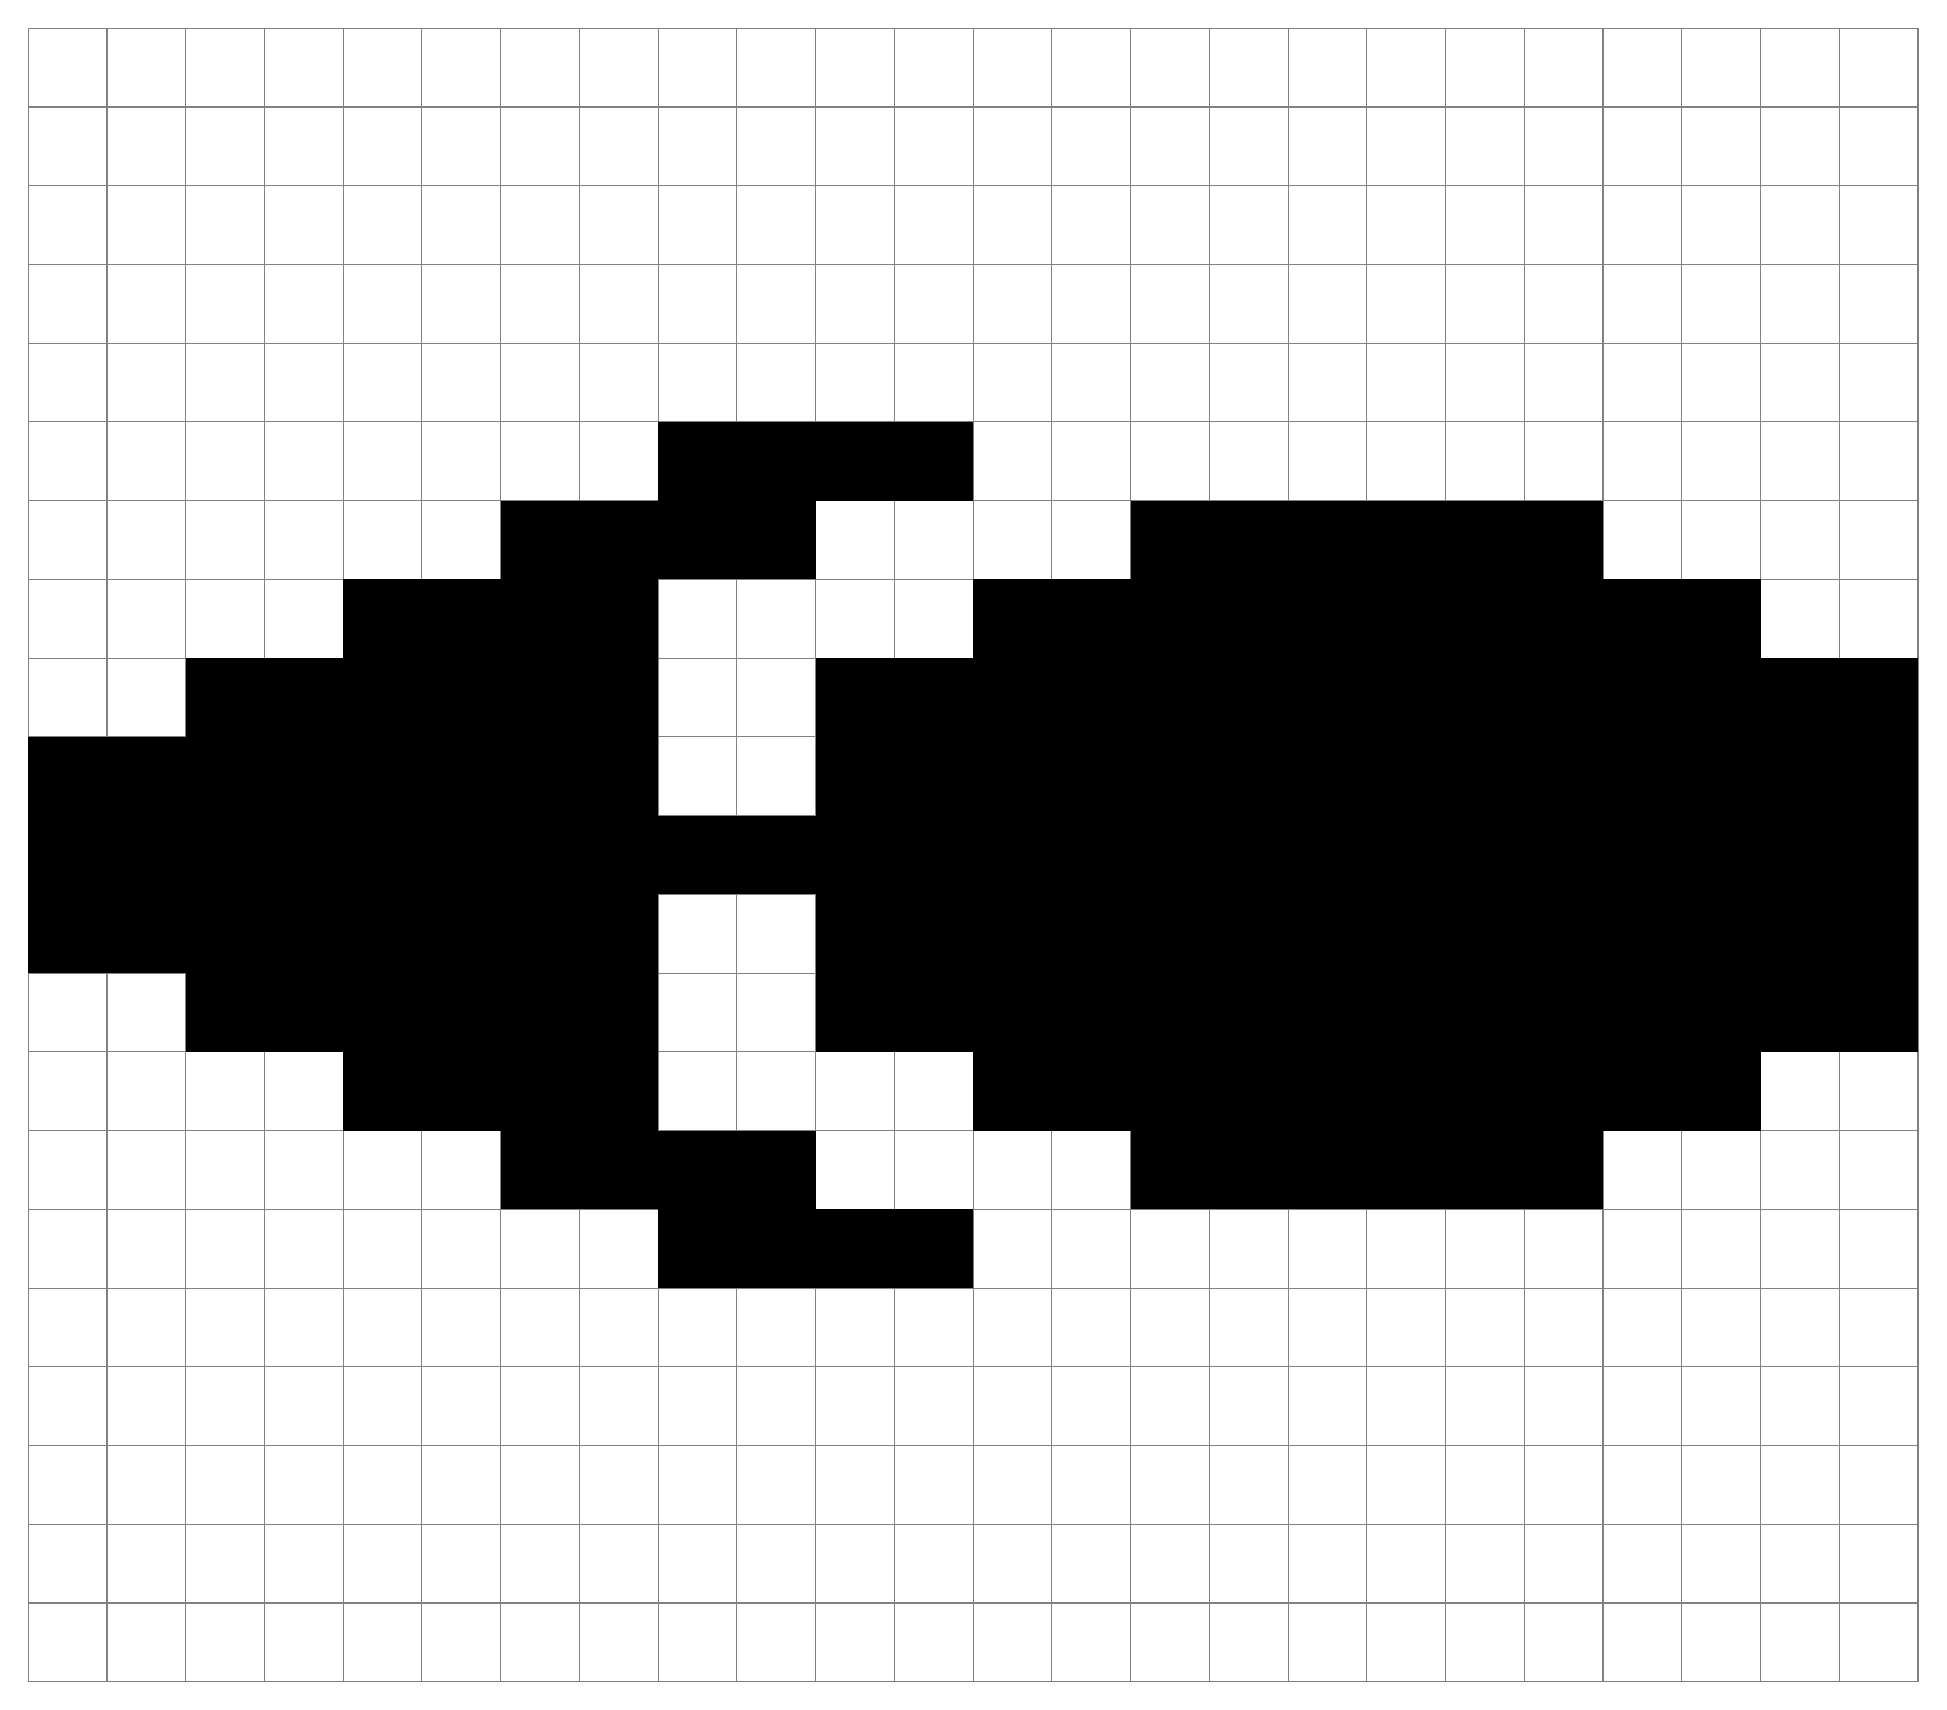
\begin{tikzpicture}

	\draw[step=1.0,gray,thin] (0,0) grid (24,21);
	\fill[\SPRITECOLOR] (8,15) rectangle ++ (1,1);
	\fill[\SPRITECOLOR] (9,15) rectangle ++ (1,1);
	\fill[\SPRITECOLOR] (10,15) rectangle ++ (1,1);
	\fill[\SPRITECOLOR] (11,15) rectangle ++ (1,1);
	\fill[\SPRITECOLOR] (6,14) rectangle ++ (1,1);
	\fill[\SPRITECOLOR] (7,14) rectangle ++ (1,1);
	\fill[\SPRITECOLOR] (8,14) rectangle ++ (1,1);
	\fill[\SPRITECOLOR] (9,14) rectangle ++ (1,1);
	\fill[\SPRITECOLOR] (14,14) rectangle ++ (1,1);
	\fill[\SPRITECOLOR] (15,14) rectangle ++ (1,1);
	\fill[\SPRITECOLOR] (16,14) rectangle ++ (1,1);
	\fill[\SPRITECOLOR] (17,14) rectangle ++ (1,1);
	\fill[\SPRITECOLOR] (18,14) rectangle ++ (1,1);
	\fill[\SPRITECOLOR] (19,14) rectangle ++ (1,1);
	\fill[\SPRITECOLOR] (4,13) rectangle ++ (1,1);
	\fill[\SPRITECOLOR] (5,13) rectangle ++ (1,1);
	\fill[\MULTICOLORONE] (6,13) rectangle ++ (1,1);
	\fill[\MULTICOLORONE] (7,13) rectangle ++ (1,1);
	\fill[\SPRITECOLOR] (12,13) rectangle ++ (1,1);
	\fill[\SPRITECOLOR] (13,13) rectangle ++ (1,1);
	\fill[\MULTICOLORTWO] (14,13) rectangle ++ (1,1);
	\fill[\MULTICOLORTWO] (15,13) rectangle ++ (1,1);
	\fill[\SPRITECOLOR] (16,13) rectangle ++ (1,1);
	\fill[\SPRITECOLOR] (17,13) rectangle ++ (1,1);
	\fill[\SPRITECOLOR] (18,13) rectangle ++ (1,1);
	\fill[\SPRITECOLOR] (19,13) rectangle ++ (1,1);
	\fill[\SPRITECOLOR] (20,13) rectangle ++ (1,1);
	\fill[\SPRITECOLOR] (21,13) rectangle ++ (1,1);
	\fill[\SPRITECOLOR] (2,12) rectangle ++ (1,1);
	\fill[\SPRITECOLOR] (3,12) rectangle ++ (1,1);
	\fill[\MULTICOLORONE] (4,12) rectangle ++ (1,1);
	\fill[\MULTICOLORONE] (5,12) rectangle ++ (1,1);
	\fill[\SPRITECOLOR] (6,12) rectangle ++ (1,1);
	\fill[\SPRITECOLOR] (7,12) rectangle ++ (1,1);
	\fill[\SPRITECOLOR] (10,12) rectangle ++ (1,1);
	\fill[\SPRITECOLOR] (11,12) rectangle ++ (1,1);
	\fill[\MULTICOLORTWO] (12,12) rectangle ++ (1,1);
	\fill[\MULTICOLORTWO] (13,12) rectangle ++ (1,1);
	\fill[\SPRITECOLOR] (14,12) rectangle ++ (1,1);
	\fill[\SPRITECOLOR] (15,12) rectangle ++ (1,1);
	\fill[\SPRITECOLOR] (16,12) rectangle ++ (1,1);
	\fill[\SPRITECOLOR] (17,12) rectangle ++ (1,1);
	\fill[\SPRITECOLOR] (18,12) rectangle ++ (1,1);
	\fill[\SPRITECOLOR] (19,12) rectangle ++ (1,1);
	\fill[\SPRITECOLOR] (20,12) rectangle ++ (1,1);
	\fill[\SPRITECOLOR] (21,12) rectangle ++ (1,1);
	\fill[\SPRITECOLOR] (22,12) rectangle ++ (1,1);
	\fill[\SPRITECOLOR] (23,12) rectangle ++ (1,1);
	\fill[\SPRITECOLOR] (0,11) rectangle ++ (1,1);
	\fill[\SPRITECOLOR] (1,11) rectangle ++ (1,1);
	\fill[\MULTICOLORONE] (2,11) rectangle ++ (1,1);
	\fill[\MULTICOLORONE] (3,11) rectangle ++ (1,1);
	\fill[\MULTICOLORONE] (4,11) rectangle ++ (1,1);
	\fill[\MULTICOLORONE] (5,11) rectangle ++ (1,1);
	\fill[\SPRITECOLOR] (6,11) rectangle ++ (1,1);
	\fill[\SPRITECOLOR] (7,11) rectangle ++ (1,1);
	\fill[\SPRITECOLOR] (10,11) rectangle ++ (1,1);
	\fill[\SPRITECOLOR] (11,11) rectangle ++ (1,1);
	\fill[\SPRITECOLOR] (12,11) rectangle ++ (1,1);
	\fill[\SPRITECOLOR] (13,11) rectangle ++ (1,1);
	\fill[\SPRITECOLOR] (14,11) rectangle ++ (1,1);
	\fill[\SPRITECOLOR] (15,11) rectangle ++ (1,1);
	\fill[\MULTICOLORONE] (16,11) rectangle ++ (1,1);
	\fill[\MULTICOLORONE] (17,11) rectangle ++ (1,1);
	\fill[\SPRITECOLOR] (18,11) rectangle ++ (1,1);
	\fill[\SPRITECOLOR] (19,11) rectangle ++ (1,1);
	\fill[\SPRITECOLOR] (20,11) rectangle ++ (1,1);
	\fill[\SPRITECOLOR] (21,11) rectangle ++ (1,1);
	\fill[\SPRITECOLOR] (22,11) rectangle ++ (1,1);
	\fill[\SPRITECOLOR] (23,11) rectangle ++ (1,1);
	\fill[\SPRITECOLOR] (0,10) rectangle ++ (1,1);
	\fill[\SPRITECOLOR] (1,10) rectangle ++ (1,1);
	\fill[\MULTICOLORONE] (2,10) rectangle ++ (1,1);
	\fill[\MULTICOLORONE] (3,10) rectangle ++ (1,1);
	\fill[\MULTICOLORONE] (4,10) rectangle ++ (1,1);
	\fill[\MULTICOLORONE] (5,10) rectangle ++ (1,1);
	\fill[\SPRITECOLOR] (6,10) rectangle ++ (1,1);
	\fill[\SPRITECOLOR] (7,10) rectangle ++ (1,1);
	\fill[\SPRITECOLOR] (8,10) rectangle ++ (1,1);
	\fill[\SPRITECOLOR] (9,10) rectangle ++ (1,1);
	\fill[\SPRITECOLOR] (10,10) rectangle ++ (1,1);
	\fill[\SPRITECOLOR] (11,10) rectangle ++ (1,1);
	\fill[\SPRITECOLOR] (12,10) rectangle ++ (1,1);
	\fill[\SPRITECOLOR] (13,10) rectangle ++ (1,1);
	\fill[\MULTICOLORONE] (14,10) rectangle ++ (1,1);
	\fill[\MULTICOLORONE] (15,10) rectangle ++ (1,1);
	\fill[\MULTICOLORONE] (16,10) rectangle ++ (1,1);
	\fill[\MULTICOLORONE] (17,10) rectangle ++ (1,1);
	\fill[\MULTICOLORONE] (18,10) rectangle ++ (1,1);
	\fill[\MULTICOLORONE] (19,10) rectangle ++ (1,1);
	\fill[\SPRITECOLOR] (20,10) rectangle ++ (1,1);
	\fill[\SPRITECOLOR] (21,10) rectangle ++ (1,1);
	\fill[\SPRITECOLOR] (22,10) rectangle ++ (1,1);
	\fill[\SPRITECOLOR] (23,10) rectangle ++ (1,1);
	\fill[\SPRITECOLOR] (0,9) rectangle ++ (1,1);
	\fill[\SPRITECOLOR] (1,9) rectangle ++ (1,1);
	\fill[\MULTICOLORONE] (2,9) rectangle ++ (1,1);
	\fill[\MULTICOLORONE] (3,9) rectangle ++ (1,1);
	\fill[\MULTICOLORONE] (4,9) rectangle ++ (1,1);
	\fill[\MULTICOLORONE] (5,9) rectangle ++ (1,1);
	\fill[\SPRITECOLOR] (6,9) rectangle ++ (1,1);
	\fill[\SPRITECOLOR] (7,9) rectangle ++ (1,1);
	\fill[\SPRITECOLOR] (10,9) rectangle ++ (1,1);
	\fill[\SPRITECOLOR] (11,9) rectangle ++ (1,1);
	\fill[\SPRITECOLOR] (12,9) rectangle ++ (1,1);
	\fill[\SPRITECOLOR] (13,9) rectangle ++ (1,1);
	\fill[\SPRITECOLOR] (14,9) rectangle ++ (1,1);
	\fill[\SPRITECOLOR] (15,9) rectangle ++ (1,1);
	\fill[\MULTICOLORONE] (16,9) rectangle ++ (1,1);
	\fill[\MULTICOLORONE] (17,9) rectangle ++ (1,1);
	\fill[\SPRITECOLOR] (18,9) rectangle ++ (1,1);
	\fill[\SPRITECOLOR] (19,9) rectangle ++ (1,1);
	\fill[\SPRITECOLOR] (20,9) rectangle ++ (1,1);
	\fill[\SPRITECOLOR] (21,9) rectangle ++ (1,1);
	\fill[\SPRITECOLOR] (22,9) rectangle ++ (1,1);
	\fill[\SPRITECOLOR] (23,9) rectangle ++ (1,1);
	\fill[\SPRITECOLOR] (2,8) rectangle ++ (1,1);
	\fill[\SPRITECOLOR] (3,8) rectangle ++ (1,1);
	\fill[\MULTICOLORONE] (4,8) rectangle ++ (1,1);
	\fill[\MULTICOLORONE] (5,8) rectangle ++ (1,1);
	\fill[\SPRITECOLOR] (6,8) rectangle ++ (1,1);
	\fill[\SPRITECOLOR] (7,8) rectangle ++ (1,1);
	\fill[\SPRITECOLOR] (10,8) rectangle ++ (1,1);
	\fill[\SPRITECOLOR] (11,8) rectangle ++ (1,1);
	\fill[\SPRITECOLOR] (12,8) rectangle ++ (1,1);
	\fill[\SPRITECOLOR] (13,8) rectangle ++ (1,1);
	\fill[\SPRITECOLOR] (14,8) rectangle ++ (1,1);
	\fill[\SPRITECOLOR] (15,8) rectangle ++ (1,1);
	\fill[\SPRITECOLOR] (16,8) rectangle ++ (1,1);
	\fill[\SPRITECOLOR] (17,8) rectangle ++ (1,1);
	\fill[\SPRITECOLOR] (18,8) rectangle ++ (1,1);
	\fill[\SPRITECOLOR] (19,8) rectangle ++ (1,1);
	\fill[\SPRITECOLOR] (20,8) rectangle ++ (1,1);
	\fill[\SPRITECOLOR] (21,8) rectangle ++ (1,1);
	\fill[\SPRITECOLOR] (22,8) rectangle ++ (1,1);
	\fill[\SPRITECOLOR] (23,8) rectangle ++ (1,1);
	\fill[\SPRITECOLOR] (4,7) rectangle ++ (1,1);
	\fill[\SPRITECOLOR] (5,7) rectangle ++ (1,1);
	\fill[\MULTICOLORONE] (6,7) rectangle ++ (1,1);
	\fill[\MULTICOLORONE] (7,7) rectangle ++ (1,1);
	\fill[\SPRITECOLOR] (12,7) rectangle ++ (1,1);
	\fill[\SPRITECOLOR] (13,7) rectangle ++ (1,1);
	\fill[\SPRITECOLOR] (14,7) rectangle ++ (1,1);
	\fill[\SPRITECOLOR] (15,7) rectangle ++ (1,1);
	\fill[\SPRITECOLOR] (16,7) rectangle ++ (1,1);
	\fill[\SPRITECOLOR] (17,7) rectangle ++ (1,1);
	\fill[\SPRITECOLOR] (18,7) rectangle ++ (1,1);
	\fill[\SPRITECOLOR] (19,7) rectangle ++ (1,1);
	\fill[\SPRITECOLOR] (20,7) rectangle ++ (1,1);
	\fill[\SPRITECOLOR] (21,7) rectangle ++ (1,1);
	\fill[\SPRITECOLOR] (6,6) rectangle ++ (1,1);
	\fill[\SPRITECOLOR] (7,6) rectangle ++ (1,1);
	\fill[\SPRITECOLOR] (8,6) rectangle ++ (1,1);
	\fill[\SPRITECOLOR] (9,6) rectangle ++ (1,1);
	\fill[\SPRITECOLOR] (14,6) rectangle ++ (1,1);
	\fill[\SPRITECOLOR] (15,6) rectangle ++ (1,1);
	\fill[\SPRITECOLOR] (16,6) rectangle ++ (1,1);
	\fill[\SPRITECOLOR] (17,6) rectangle ++ (1,1);
	\fill[\SPRITECOLOR] (18,6) rectangle ++ (1,1);
	\fill[\SPRITECOLOR] (19,6) rectangle ++ (1,1);
	\fill[\SPRITECOLOR] (8,5) rectangle ++ (1,1);
	\fill[\SPRITECOLOR] (9,5) rectangle ++ (1,1);
	\fill[\SPRITECOLOR] (10,5) rectangle ++ (1,1);
	\fill[\SPRITECOLOR] (11,5) rectangle ++ (1,1);

      \end{tikzpicture}
    \end{adjustbox}
  }\caption{UGLY\_GILBY7}
\end{figure}

	\end{subfigure}
} & 
\makecell[l]{
	\begin{subfigure}{0.3\textwidth}
    \def\MULTICOLORONE{gray}
    \def\MULTICOLORTWO{white}
    \def\SPRITECOLOR{red}
		
\begin{figure}[H]
  {
    \setlength{\tabcolsep}{3.0pt}
    \setlength\cmidrulewidth{\heavyrulewidth} % Make cmidrule = 
    \begin{adjustbox}{width=3cm,center}
      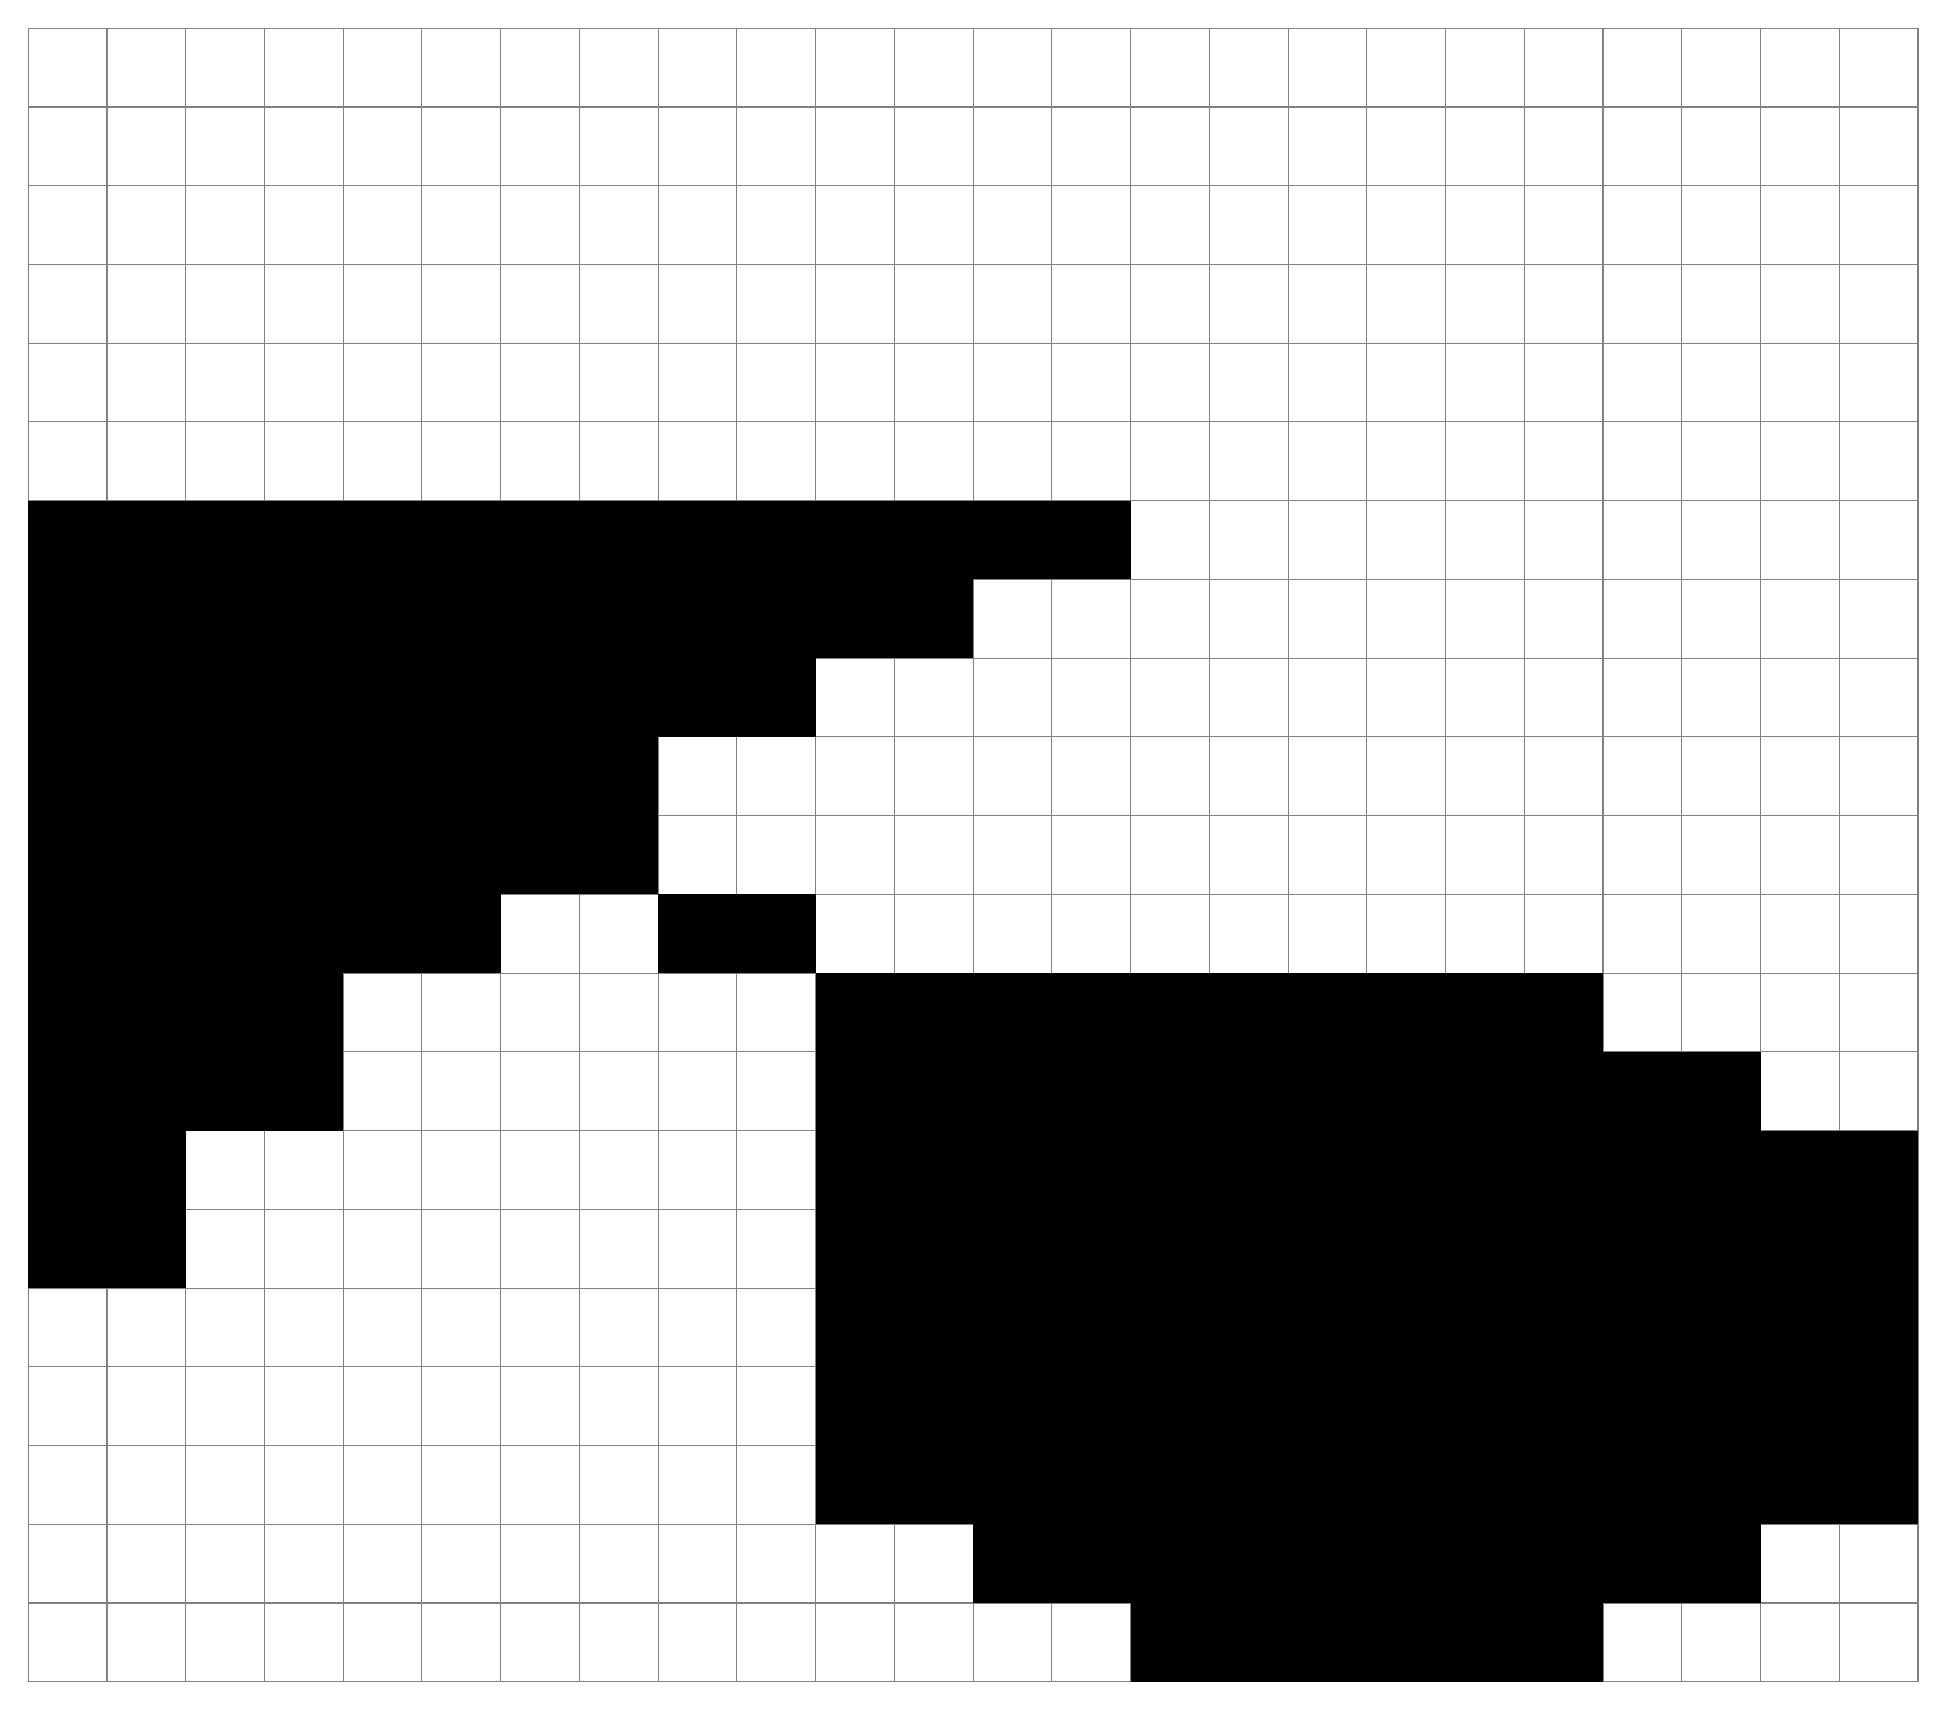
\begin{tikzpicture}

	\draw[step=1.0,gray,thin] (0,0) grid (24,21);
	\fill[\SPRITECOLOR] (0,14) rectangle ++ (1,1);
	\fill[\SPRITECOLOR] (1,14) rectangle ++ (1,1);
	\fill[\SPRITECOLOR] (2,14) rectangle ++ (1,1);
	\fill[\SPRITECOLOR] (3,14) rectangle ++ (1,1);
	\fill[\SPRITECOLOR] (4,14) rectangle ++ (1,1);
	\fill[\SPRITECOLOR] (5,14) rectangle ++ (1,1);
	\fill[\SPRITECOLOR] (6,14) rectangle ++ (1,1);
	\fill[\SPRITECOLOR] (7,14) rectangle ++ (1,1);
	\fill[\SPRITECOLOR] (8,14) rectangle ++ (1,1);
	\fill[\SPRITECOLOR] (9,14) rectangle ++ (1,1);
	\fill[\SPRITECOLOR] (10,14) rectangle ++ (1,1);
	\fill[\SPRITECOLOR] (11,14) rectangle ++ (1,1);
	\fill[\SPRITECOLOR] (12,14) rectangle ++ (1,1);
	\fill[\SPRITECOLOR] (13,14) rectangle ++ (1,1);
	\fill[\SPRITECOLOR] (0,13) rectangle ++ (1,1);
	\fill[\SPRITECOLOR] (1,13) rectangle ++ (1,1);
	\fill[\MULTICOLORONE] (2,13) rectangle ++ (1,1);
	\fill[\MULTICOLORONE] (3,13) rectangle ++ (1,1);
	\fill[\MULTICOLORONE] (4,13) rectangle ++ (1,1);
	\fill[\MULTICOLORONE] (5,13) rectangle ++ (1,1);
	\fill[\MULTICOLORONE] (6,13) rectangle ++ (1,1);
	\fill[\MULTICOLORONE] (7,13) rectangle ++ (1,1);
	\fill[\MULTICOLORONE] (8,13) rectangle ++ (1,1);
	\fill[\MULTICOLORONE] (9,13) rectangle ++ (1,1);
	\fill[\SPRITECOLOR] (10,13) rectangle ++ (1,1);
	\fill[\SPRITECOLOR] (11,13) rectangle ++ (1,1);
	\fill[\SPRITECOLOR] (0,12) rectangle ++ (1,1);
	\fill[\SPRITECOLOR] (1,12) rectangle ++ (1,1);
	\fill[\MULTICOLORONE] (2,12) rectangle ++ (1,1);
	\fill[\MULTICOLORONE] (3,12) rectangle ++ (1,1);
	\fill[\MULTICOLORONE] (4,12) rectangle ++ (1,1);
	\fill[\MULTICOLORONE] (5,12) rectangle ++ (1,1);
	\fill[\SPRITECOLOR] (6,12) rectangle ++ (1,1);
	\fill[\SPRITECOLOR] (7,12) rectangle ++ (1,1);
	\fill[\SPRITECOLOR] (8,12) rectangle ++ (1,1);
	\fill[\SPRITECOLOR] (9,12) rectangle ++ (1,1);
	\fill[\SPRITECOLOR] (0,11) rectangle ++ (1,1);
	\fill[\SPRITECOLOR] (1,11) rectangle ++ (1,1);
	\fill[\MULTICOLORONE] (2,11) rectangle ++ (1,1);
	\fill[\MULTICOLORONE] (3,11) rectangle ++ (1,1);
	\fill[\SPRITECOLOR] (4,11) rectangle ++ (1,1);
	\fill[\SPRITECOLOR] (5,11) rectangle ++ (1,1);
	\fill[\SPRITECOLOR] (6,11) rectangle ++ (1,1);
	\fill[\SPRITECOLOR] (7,11) rectangle ++ (1,1);
	\fill[\SPRITECOLOR] (0,10) rectangle ++ (1,1);
	\fill[\SPRITECOLOR] (1,10) rectangle ++ (1,1);
	\fill[\MULTICOLORONE] (2,10) rectangle ++ (1,1);
	\fill[\MULTICOLORONE] (3,10) rectangle ++ (1,1);
	\fill[\SPRITECOLOR] (4,10) rectangle ++ (1,1);
	\fill[\SPRITECOLOR] (5,10) rectangle ++ (1,1);
	\fill[\SPRITECOLOR] (6,10) rectangle ++ (1,1);
	\fill[\SPRITECOLOR] (7,10) rectangle ++ (1,1);
	\fill[\SPRITECOLOR] (0,9) rectangle ++ (1,1);
	\fill[\SPRITECOLOR] (1,9) rectangle ++ (1,1);
	\fill[\MULTICOLORONE] (2,9) rectangle ++ (1,1);
	\fill[\MULTICOLORONE] (3,9) rectangle ++ (1,1);
	\fill[\SPRITECOLOR] (4,9) rectangle ++ (1,1);
	\fill[\SPRITECOLOR] (5,9) rectangle ++ (1,1);
	\fill[\SPRITECOLOR] (8,9) rectangle ++ (1,1);
	\fill[\SPRITECOLOR] (9,9) rectangle ++ (1,1);
	\fill[\SPRITECOLOR] (0,8) rectangle ++ (1,1);
	\fill[\SPRITECOLOR] (1,8) rectangle ++ (1,1);
	\fill[\SPRITECOLOR] (2,8) rectangle ++ (1,1);
	\fill[\SPRITECOLOR] (3,8) rectangle ++ (1,1);
	\fill[\SPRITECOLOR] (10,8) rectangle ++ (1,1);
	\fill[\SPRITECOLOR] (11,8) rectangle ++ (1,1);
	\fill[\SPRITECOLOR] (12,8) rectangle ++ (1,1);
	\fill[\SPRITECOLOR] (13,8) rectangle ++ (1,1);
	\fill[\SPRITECOLOR] (14,8) rectangle ++ (1,1);
	\fill[\SPRITECOLOR] (15,8) rectangle ++ (1,1);
	\fill[\SPRITECOLOR] (16,8) rectangle ++ (1,1);
	\fill[\SPRITECOLOR] (17,8) rectangle ++ (1,1);
	\fill[\SPRITECOLOR] (18,8) rectangle ++ (1,1);
	\fill[\SPRITECOLOR] (19,8) rectangle ++ (1,1);
	\fill[\SPRITECOLOR] (0,7) rectangle ++ (1,1);
	\fill[\SPRITECOLOR] (1,7) rectangle ++ (1,1);
	\fill[\SPRITECOLOR] (2,7) rectangle ++ (1,1);
	\fill[\SPRITECOLOR] (3,7) rectangle ++ (1,1);
	\fill[\SPRITECOLOR] (10,7) rectangle ++ (1,1);
	\fill[\SPRITECOLOR] (11,7) rectangle ++ (1,1);
	\fill[\SPRITECOLOR] (12,7) rectangle ++ (1,1);
	\fill[\SPRITECOLOR] (13,7) rectangle ++ (1,1);
	\fill[\MULTICOLORTWO] (14,7) rectangle ++ (1,1);
	\fill[\MULTICOLORTWO] (15,7) rectangle ++ (1,1);
	\fill[\SPRITECOLOR] (16,7) rectangle ++ (1,1);
	\fill[\SPRITECOLOR] (17,7) rectangle ++ (1,1);
	\fill[\SPRITECOLOR] (18,7) rectangle ++ (1,1);
	\fill[\SPRITECOLOR] (19,7) rectangle ++ (1,1);
	\fill[\SPRITECOLOR] (20,7) rectangle ++ (1,1);
	\fill[\SPRITECOLOR] (21,7) rectangle ++ (1,1);
	\fill[\SPRITECOLOR] (0,6) rectangle ++ (1,1);
	\fill[\SPRITECOLOR] (1,6) rectangle ++ (1,1);
	\fill[\SPRITECOLOR] (10,6) rectangle ++ (1,1);
	\fill[\SPRITECOLOR] (11,6) rectangle ++ (1,1);
	\fill[\MULTICOLORTWO] (12,6) rectangle ++ (1,1);
	\fill[\MULTICOLORTWO] (13,6) rectangle ++ (1,1);
	\fill[\SPRITECOLOR] (14,6) rectangle ++ (1,1);
	\fill[\SPRITECOLOR] (15,6) rectangle ++ (1,1);
	\fill[\SPRITECOLOR] (16,6) rectangle ++ (1,1);
	\fill[\SPRITECOLOR] (17,6) rectangle ++ (1,1);
	\fill[\SPRITECOLOR] (18,6) rectangle ++ (1,1);
	\fill[\SPRITECOLOR] (19,6) rectangle ++ (1,1);
	\fill[\SPRITECOLOR] (20,6) rectangle ++ (1,1);
	\fill[\SPRITECOLOR] (21,6) rectangle ++ (1,1);
	\fill[\SPRITECOLOR] (22,6) rectangle ++ (1,1);
	\fill[\SPRITECOLOR] (23,6) rectangle ++ (1,1);
	\fill[\SPRITECOLOR] (0,5) rectangle ++ (1,1);
	\fill[\SPRITECOLOR] (1,5) rectangle ++ (1,1);
	\fill[\SPRITECOLOR] (10,5) rectangle ++ (1,1);
	\fill[\SPRITECOLOR] (11,5) rectangle ++ (1,1);
	\fill[\SPRITECOLOR] (12,5) rectangle ++ (1,1);
	\fill[\SPRITECOLOR] (13,5) rectangle ++ (1,1);
	\fill[\SPRITECOLOR] (14,5) rectangle ++ (1,1);
	\fill[\SPRITECOLOR] (15,5) rectangle ++ (1,1);
	\fill[\MULTICOLORONE] (16,5) rectangle ++ (1,1);
	\fill[\MULTICOLORONE] (17,5) rectangle ++ (1,1);
	\fill[\SPRITECOLOR] (18,5) rectangle ++ (1,1);
	\fill[\SPRITECOLOR] (19,5) rectangle ++ (1,1);
	\fill[\SPRITECOLOR] (20,5) rectangle ++ (1,1);
	\fill[\SPRITECOLOR] (21,5) rectangle ++ (1,1);
	\fill[\SPRITECOLOR] (22,5) rectangle ++ (1,1);
	\fill[\SPRITECOLOR] (23,5) rectangle ++ (1,1);
	\fill[\SPRITECOLOR] (10,4) rectangle ++ (1,1);
	\fill[\SPRITECOLOR] (11,4) rectangle ++ (1,1);
	\fill[\SPRITECOLOR] (12,4) rectangle ++ (1,1);
	\fill[\SPRITECOLOR] (13,4) rectangle ++ (1,1);
	\fill[\MULTICOLORONE] (14,4) rectangle ++ (1,1);
	\fill[\MULTICOLORONE] (15,4) rectangle ++ (1,1);
	\fill[\MULTICOLORONE] (16,4) rectangle ++ (1,1);
	\fill[\MULTICOLORONE] (17,4) rectangle ++ (1,1);
	\fill[\MULTICOLORONE] (18,4) rectangle ++ (1,1);
	\fill[\MULTICOLORONE] (19,4) rectangle ++ (1,1);
	\fill[\SPRITECOLOR] (20,4) rectangle ++ (1,1);
	\fill[\SPRITECOLOR] (21,4) rectangle ++ (1,1);
	\fill[\SPRITECOLOR] (22,4) rectangle ++ (1,1);
	\fill[\SPRITECOLOR] (23,4) rectangle ++ (1,1);
	\fill[\SPRITECOLOR] (10,3) rectangle ++ (1,1);
	\fill[\SPRITECOLOR] (11,3) rectangle ++ (1,1);
	\fill[\SPRITECOLOR] (12,3) rectangle ++ (1,1);
	\fill[\SPRITECOLOR] (13,3) rectangle ++ (1,1);
	\fill[\SPRITECOLOR] (14,3) rectangle ++ (1,1);
	\fill[\SPRITECOLOR] (15,3) rectangle ++ (1,1);
	\fill[\MULTICOLORONE] (16,3) rectangle ++ (1,1);
	\fill[\MULTICOLORONE] (17,3) rectangle ++ (1,1);
	\fill[\SPRITECOLOR] (18,3) rectangle ++ (1,1);
	\fill[\SPRITECOLOR] (19,3) rectangle ++ (1,1);
	\fill[\SPRITECOLOR] (20,3) rectangle ++ (1,1);
	\fill[\SPRITECOLOR] (21,3) rectangle ++ (1,1);
	\fill[\SPRITECOLOR] (22,3) rectangle ++ (1,1);
	\fill[\SPRITECOLOR] (23,3) rectangle ++ (1,1);
	\fill[\SPRITECOLOR] (10,2) rectangle ++ (1,1);
	\fill[\SPRITECOLOR] (11,2) rectangle ++ (1,1);
	\fill[\SPRITECOLOR] (12,2) rectangle ++ (1,1);
	\fill[\SPRITECOLOR] (13,2) rectangle ++ (1,1);
	\fill[\SPRITECOLOR] (14,2) rectangle ++ (1,1);
	\fill[\SPRITECOLOR] (15,2) rectangle ++ (1,1);
	\fill[\SPRITECOLOR] (16,2) rectangle ++ (1,1);
	\fill[\SPRITECOLOR] (17,2) rectangle ++ (1,1);
	\fill[\SPRITECOLOR] (18,2) rectangle ++ (1,1);
	\fill[\SPRITECOLOR] (19,2) rectangle ++ (1,1);
	\fill[\SPRITECOLOR] (20,2) rectangle ++ (1,1);
	\fill[\SPRITECOLOR] (21,2) rectangle ++ (1,1);
	\fill[\SPRITECOLOR] (22,2) rectangle ++ (1,1);
	\fill[\SPRITECOLOR] (23,2) rectangle ++ (1,1);
	\fill[\SPRITECOLOR] (12,1) rectangle ++ (1,1);
	\fill[\SPRITECOLOR] (13,1) rectangle ++ (1,1);
	\fill[\SPRITECOLOR] (14,1) rectangle ++ (1,1);
	\fill[\SPRITECOLOR] (15,1) rectangle ++ (1,1);
	\fill[\SPRITECOLOR] (16,1) rectangle ++ (1,1);
	\fill[\SPRITECOLOR] (17,1) rectangle ++ (1,1);
	\fill[\SPRITECOLOR] (18,1) rectangle ++ (1,1);
	\fill[\SPRITECOLOR] (19,1) rectangle ++ (1,1);
	\fill[\SPRITECOLOR] (20,1) rectangle ++ (1,1);
	\fill[\SPRITECOLOR] (21,1) rectangle ++ (1,1);
	\fill[\SPRITECOLOR] (14,0) rectangle ++ (1,1);
	\fill[\SPRITECOLOR] (15,0) rectangle ++ (1,1);
	\fill[\SPRITECOLOR] (16,0) rectangle ++ (1,1);
	\fill[\SPRITECOLOR] (17,0) rectangle ++ (1,1);
	\fill[\SPRITECOLOR] (18,0) rectangle ++ (1,1);
	\fill[\SPRITECOLOR] (19,0) rectangle ++ (1,1);

      \end{tikzpicture}
    \end{adjustbox}
  }\caption{UGLY\_GILBY8}
\end{figure}

	\end{subfigure}
} \\ 
        \addlinespace
        \bottomrule
      \end{tabular}
    \end{adjustbox}
  }\caption{There is no excuse for this.}
\end{figure}

\section{IBalls}

\begin{figure}[H]
  {
    \setlength{\tabcolsep}{1.0pt}
    \setlength\cmidrulewidth{\heavyrulewidth} % Make cmidrule = 
    \begin{adjustbox}{width=14cm,center}
      \begin{tabular}{ccccccc}
        \toprule
        IBall & Another One & A Third & One More & \\
        \midrule
        \midrule
\makecell[l]{
	\begin{subfigure}{0.3\textwidth}
    \def\MULTICOLORONE{gray}
    \def\MULTICOLORTWO{white}
    \def\SPRITECOLOR{black}
		
\begin{figure}[H]
  {
    \setlength{\tabcolsep}{3.0pt}
    \setlength\cmidrulewidth{\heavyrulewidth} % Make cmidrule = 
    \begin{adjustbox}{width=3cm,center}
      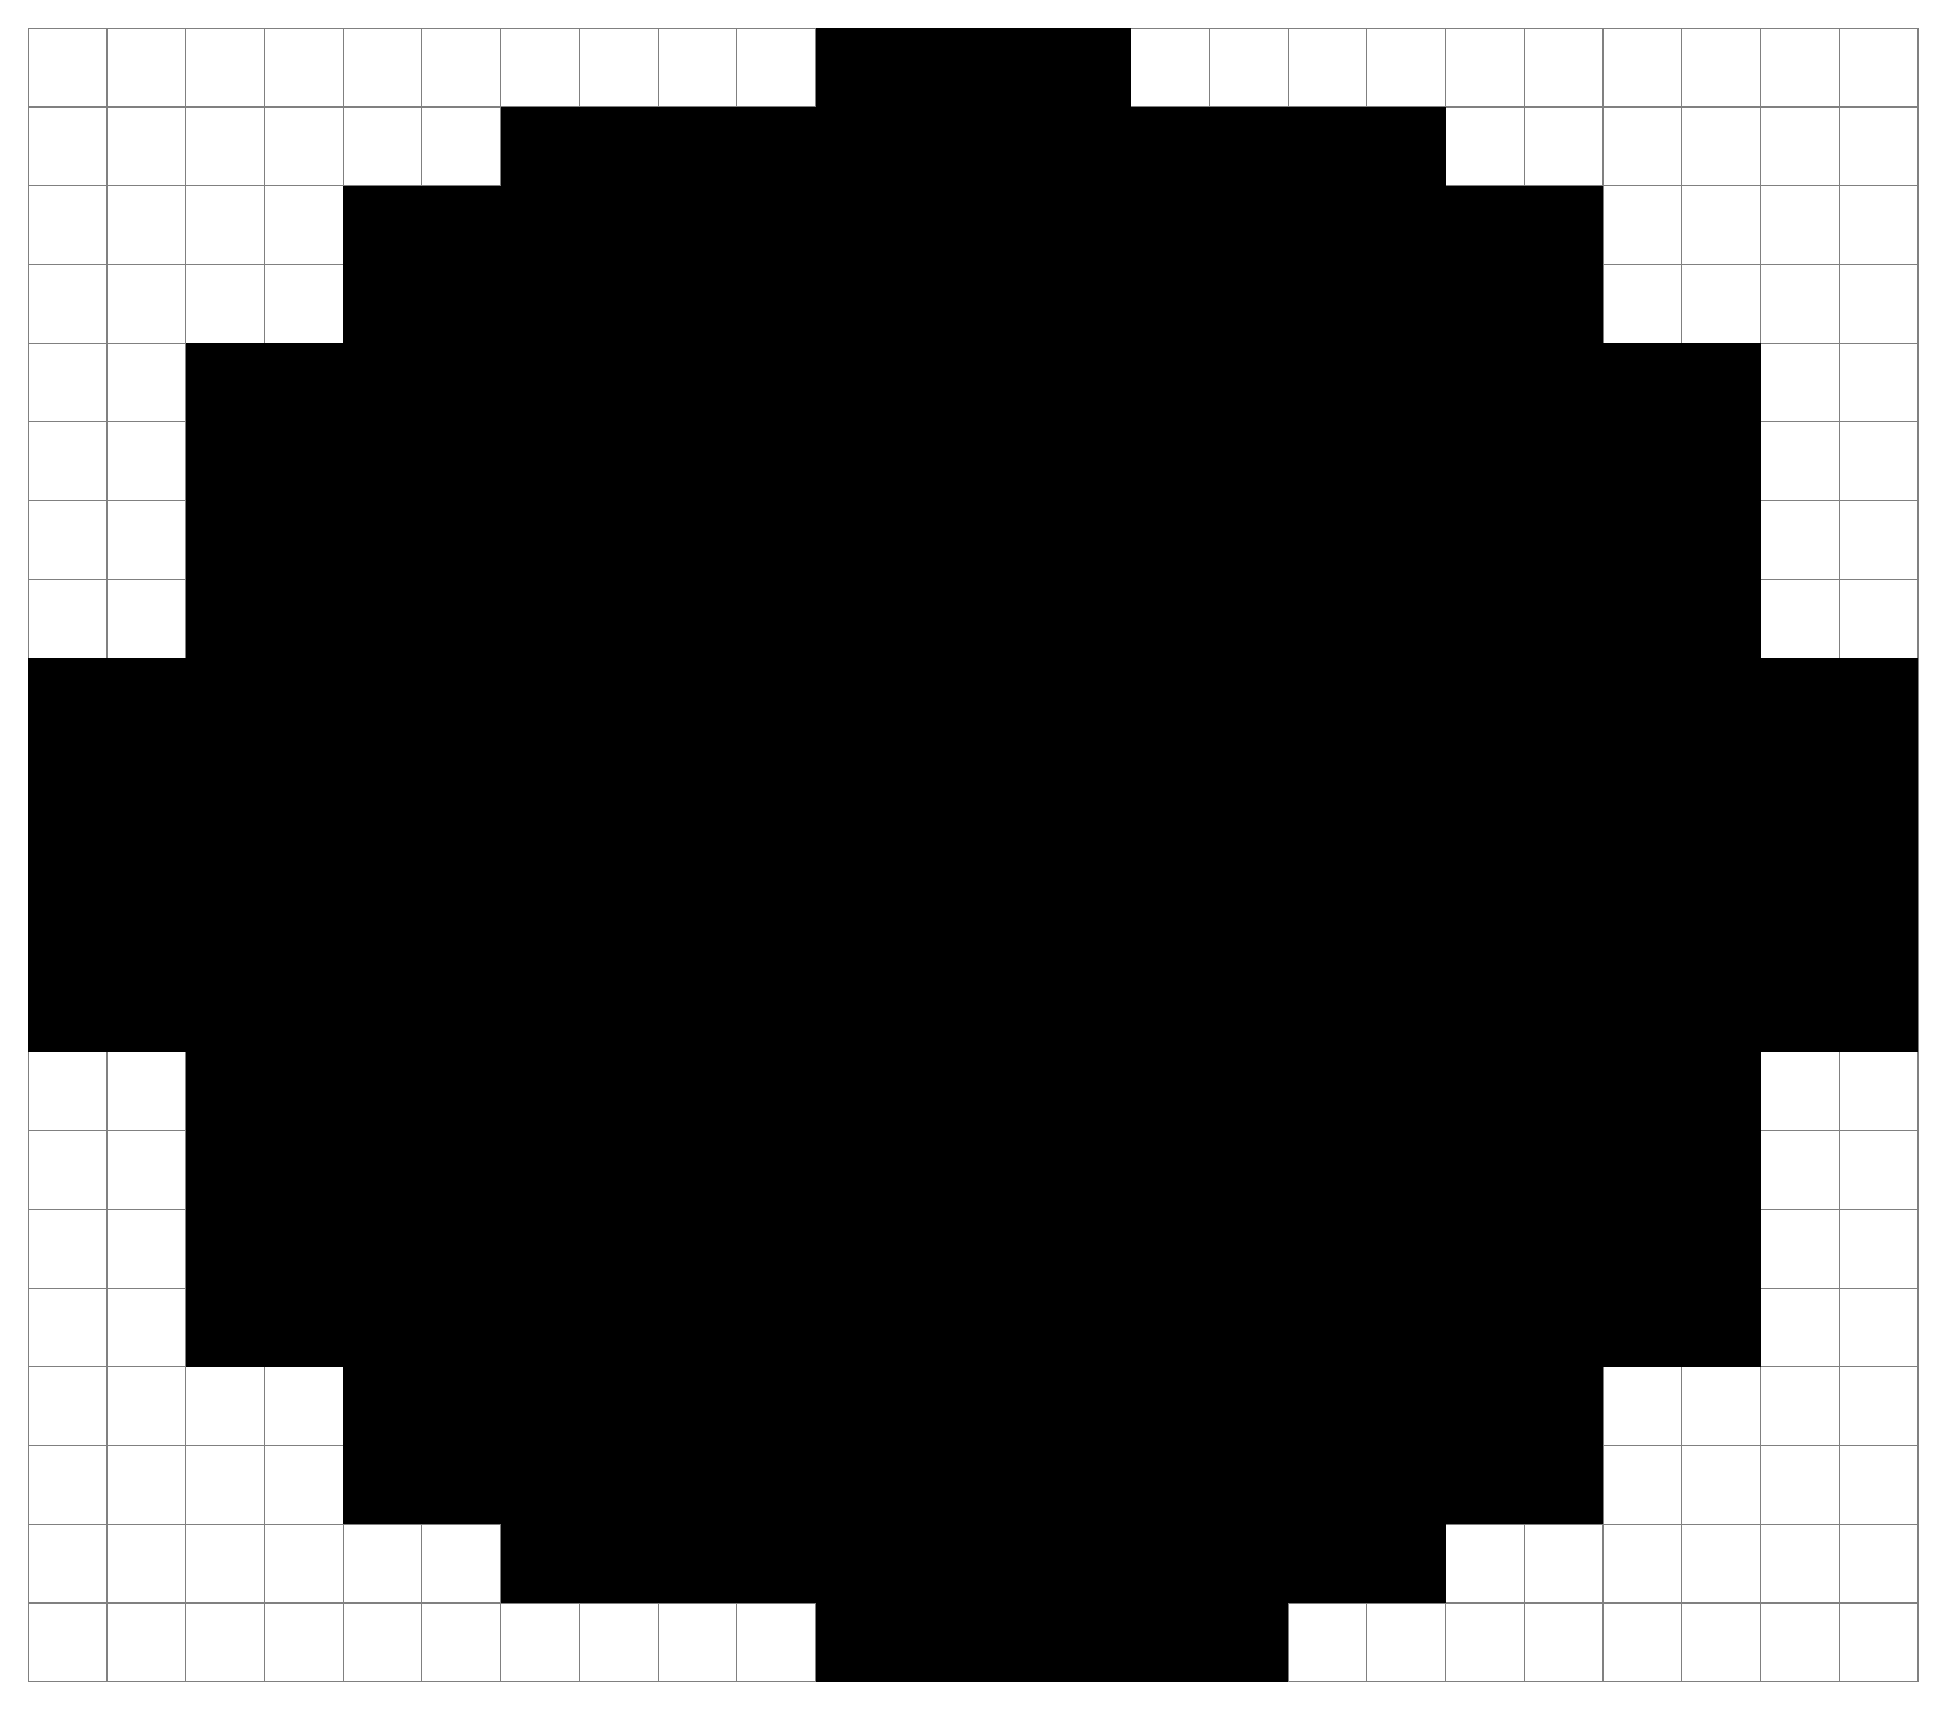
\begin{tikzpicture}

	\draw[step=1.0,gray,thin] (0,0) grid (24,21);
	\fill[\SPRITECOLOR] (10,20) rectangle ++ (1,1);
	\fill[\SPRITECOLOR] (11,20) rectangle ++ (1,1);
	\fill[\SPRITECOLOR] (12,20) rectangle ++ (1,1);
	\fill[\SPRITECOLOR] (13,20) rectangle ++ (1,1);
	\fill[\SPRITECOLOR] (6,19) rectangle ++ (1,1);
	\fill[\SPRITECOLOR] (7,19) rectangle ++ (1,1);
	\fill[\SPRITECOLOR] (8,19) rectangle ++ (1,1);
	\fill[\SPRITECOLOR] (9,19) rectangle ++ (1,1);
	\fill[\SPRITECOLOR] (10,19) rectangle ++ (1,1);
	\fill[\SPRITECOLOR] (11,19) rectangle ++ (1,1);
	\fill[\SPRITECOLOR] (12,19) rectangle ++ (1,1);
	\fill[\SPRITECOLOR] (13,19) rectangle ++ (1,1);
	\fill[\SPRITECOLOR] (14,19) rectangle ++ (1,1);
	\fill[\SPRITECOLOR] (15,19) rectangle ++ (1,1);
	\fill[\SPRITECOLOR] (16,19) rectangle ++ (1,1);
	\fill[\SPRITECOLOR] (17,19) rectangle ++ (1,1);
	\fill[\SPRITECOLOR] (4,18) rectangle ++ (1,1);
	\fill[\SPRITECOLOR] (5,18) rectangle ++ (1,1);
	\fill[\SPRITECOLOR] (6,18) rectangle ++ (1,1);
	\fill[\SPRITECOLOR] (7,18) rectangle ++ (1,1);
	\fill[\SPRITECOLOR] (8,18) rectangle ++ (1,1);
	\fill[\SPRITECOLOR] (9,18) rectangle ++ (1,1);
	\fill[\SPRITECOLOR] (10,18) rectangle ++ (1,1);
	\fill[\SPRITECOLOR] (11,18) rectangle ++ (1,1);
	\fill[\SPRITECOLOR] (12,18) rectangle ++ (1,1);
	\fill[\SPRITECOLOR] (13,18) rectangle ++ (1,1);
	\fill[\SPRITECOLOR] (14,18) rectangle ++ (1,1);
	\fill[\SPRITECOLOR] (15,18) rectangle ++ (1,1);
	\fill[\SPRITECOLOR] (16,18) rectangle ++ (1,1);
	\fill[\SPRITECOLOR] (17,18) rectangle ++ (1,1);
	\fill[\SPRITECOLOR] (18,18) rectangle ++ (1,1);
	\fill[\SPRITECOLOR] (19,18) rectangle ++ (1,1);
	\fill[\SPRITECOLOR] (4,17) rectangle ++ (1,1);
	\fill[\SPRITECOLOR] (5,17) rectangle ++ (1,1);
	\fill[\SPRITECOLOR] (6,17) rectangle ++ (1,1);
	\fill[\SPRITECOLOR] (7,17) rectangle ++ (1,1);
	\fill[\MULTICOLORTWO] (8,17) rectangle ++ (1,1);
	\fill[\MULTICOLORTWO] (9,17) rectangle ++ (1,1);
	\fill[\SPRITECOLOR] (10,17) rectangle ++ (1,1);
	\fill[\SPRITECOLOR] (11,17) rectangle ++ (1,1);
	\fill[\SPRITECOLOR] (12,17) rectangle ++ (1,1);
	\fill[\SPRITECOLOR] (13,17) rectangle ++ (1,1);
	\fill[\SPRITECOLOR] (14,17) rectangle ++ (1,1);
	\fill[\SPRITECOLOR] (15,17) rectangle ++ (1,1);
	\fill[\SPRITECOLOR] (16,17) rectangle ++ (1,1);
	\fill[\SPRITECOLOR] (17,17) rectangle ++ (1,1);
	\fill[\SPRITECOLOR] (18,17) rectangle ++ (1,1);
	\fill[\SPRITECOLOR] (19,17) rectangle ++ (1,1);
	\fill[\SPRITECOLOR] (2,16) rectangle ++ (1,1);
	\fill[\SPRITECOLOR] (3,16) rectangle ++ (1,1);
	\fill[\SPRITECOLOR] (4,16) rectangle ++ (1,1);
	\fill[\SPRITECOLOR] (5,16) rectangle ++ (1,1);
	\fill[\MULTICOLORTWO] (6,16) rectangle ++ (1,1);
	\fill[\MULTICOLORTWO] (7,16) rectangle ++ (1,1);
	\fill[\SPRITECOLOR] (8,16) rectangle ++ (1,1);
	\fill[\SPRITECOLOR] (9,16) rectangle ++ (1,1);
	\fill[\SPRITECOLOR] (10,16) rectangle ++ (1,1);
	\fill[\SPRITECOLOR] (11,16) rectangle ++ (1,1);
	\fill[\SPRITECOLOR] (12,16) rectangle ++ (1,1);
	\fill[\SPRITECOLOR] (13,16) rectangle ++ (1,1);
	\fill[\SPRITECOLOR] (14,16) rectangle ++ (1,1);
	\fill[\SPRITECOLOR] (15,16) rectangle ++ (1,1);
	\fill[\SPRITECOLOR] (16,16) rectangle ++ (1,1);
	\fill[\SPRITECOLOR] (17,16) rectangle ++ (1,1);
	\fill[\SPRITECOLOR] (18,16) rectangle ++ (1,1);
	\fill[\SPRITECOLOR] (19,16) rectangle ++ (1,1);
	\fill[\SPRITECOLOR] (20,16) rectangle ++ (1,1);
	\fill[\SPRITECOLOR] (21,16) rectangle ++ (1,1);
	\fill[\SPRITECOLOR] (2,15) rectangle ++ (1,1);
	\fill[\SPRITECOLOR] (3,15) rectangle ++ (1,1);
	\fill[\SPRITECOLOR] (4,15) rectangle ++ (1,1);
	\fill[\SPRITECOLOR] (5,15) rectangle ++ (1,1);
	\fill[\SPRITECOLOR] (6,15) rectangle ++ (1,1);
	\fill[\SPRITECOLOR] (7,15) rectangle ++ (1,1);
	\fill[\SPRITECOLOR] (8,15) rectangle ++ (1,1);
	\fill[\SPRITECOLOR] (9,15) rectangle ++ (1,1);
	\fill[\SPRITECOLOR] (10,15) rectangle ++ (1,1);
	\fill[\SPRITECOLOR] (11,15) rectangle ++ (1,1);
	\fill[\SPRITECOLOR] (12,15) rectangle ++ (1,1);
	\fill[\SPRITECOLOR] (13,15) rectangle ++ (1,1);
	\fill[\SPRITECOLOR] (14,15) rectangle ++ (1,1);
	\fill[\SPRITECOLOR] (15,15) rectangle ++ (1,1);
	\fill[\SPRITECOLOR] (16,15) rectangle ++ (1,1);
	\fill[\SPRITECOLOR] (17,15) rectangle ++ (1,1);
	\fill[\SPRITECOLOR] (18,15) rectangle ++ (1,1);
	\fill[\SPRITECOLOR] (19,15) rectangle ++ (1,1);
	\fill[\SPRITECOLOR] (20,15) rectangle ++ (1,1);
	\fill[\SPRITECOLOR] (21,15) rectangle ++ (1,1);
	\fill[\SPRITECOLOR] (2,14) rectangle ++ (1,1);
	\fill[\SPRITECOLOR] (3,14) rectangle ++ (1,1);
	\fill[\SPRITECOLOR] (4,14) rectangle ++ (1,1);
	\fill[\SPRITECOLOR] (5,14) rectangle ++ (1,1);
	\fill[\SPRITECOLOR] (6,14) rectangle ++ (1,1);
	\fill[\SPRITECOLOR] (7,14) rectangle ++ (1,1);
	\fill[\SPRITECOLOR] (8,14) rectangle ++ (1,1);
	\fill[\SPRITECOLOR] (9,14) rectangle ++ (1,1);
	\fill[\SPRITECOLOR] (10,14) rectangle ++ (1,1);
	\fill[\SPRITECOLOR] (11,14) rectangle ++ (1,1);
	\fill[\SPRITECOLOR] (12,14) rectangle ++ (1,1);
	\fill[\SPRITECOLOR] (13,14) rectangle ++ (1,1);
	\fill[\SPRITECOLOR] (14,14) rectangle ++ (1,1);
	\fill[\SPRITECOLOR] (15,14) rectangle ++ (1,1);
	\fill[\SPRITECOLOR] (16,14) rectangle ++ (1,1);
	\fill[\SPRITECOLOR] (17,14) rectangle ++ (1,1);
	\fill[\SPRITECOLOR] (18,14) rectangle ++ (1,1);
	\fill[\SPRITECOLOR] (19,14) rectangle ++ (1,1);
	\fill[\SPRITECOLOR] (20,14) rectangle ++ (1,1);
	\fill[\SPRITECOLOR] (21,14) rectangle ++ (1,1);
	\fill[\SPRITECOLOR] (2,13) rectangle ++ (1,1);
	\fill[\SPRITECOLOR] (3,13) rectangle ++ (1,1);
	\fill[\SPRITECOLOR] (4,13) rectangle ++ (1,1);
	\fill[\SPRITECOLOR] (5,13) rectangle ++ (1,1);
	\fill[\SPRITECOLOR] (6,13) rectangle ++ (1,1);
	\fill[\SPRITECOLOR] (7,13) rectangle ++ (1,1);
	\fill[\MULTICOLORTWO] (8,13) rectangle ++ (1,1);
	\fill[\MULTICOLORTWO] (9,13) rectangle ++ (1,1);
	\fill[\MULTICOLORTWO] (10,13) rectangle ++ (1,1);
	\fill[\MULTICOLORTWO] (11,13) rectangle ++ (1,1);
	\fill[\MULTICOLORTWO] (12,13) rectangle ++ (1,1);
	\fill[\MULTICOLORTWO] (13,13) rectangle ++ (1,1);
	\fill[\MULTICOLORTWO] (14,13) rectangle ++ (1,1);
	\fill[\MULTICOLORTWO] (15,13) rectangle ++ (1,1);
	\fill[\SPRITECOLOR] (16,13) rectangle ++ (1,1);
	\fill[\SPRITECOLOR] (17,13) rectangle ++ (1,1);
	\fill[\SPRITECOLOR] (18,13) rectangle ++ (1,1);
	\fill[\SPRITECOLOR] (19,13) rectangle ++ (1,1);
	\fill[\SPRITECOLOR] (20,13) rectangle ++ (1,1);
	\fill[\SPRITECOLOR] (21,13) rectangle ++ (1,1);
	\fill[\SPRITECOLOR] (0,12) rectangle ++ (1,1);
	\fill[\SPRITECOLOR] (1,12) rectangle ++ (1,1);
	\fill[\SPRITECOLOR] (2,12) rectangle ++ (1,1);
	\fill[\SPRITECOLOR] (3,12) rectangle ++ (1,1);
	\fill[\SPRITECOLOR] (4,12) rectangle ++ (1,1);
	\fill[\SPRITECOLOR] (5,12) rectangle ++ (1,1);
	\fill[\MULTICOLORTWO] (6,12) rectangle ++ (1,1);
	\fill[\MULTICOLORTWO] (7,12) rectangle ++ (1,1);
	\fill[\MULTICOLORTWO] (8,12) rectangle ++ (1,1);
	\fill[\MULTICOLORTWO] (9,12) rectangle ++ (1,1);
	\fill[\MULTICOLORTWO] (10,12) rectangle ++ (1,1);
	\fill[\MULTICOLORTWO] (11,12) rectangle ++ (1,1);
	\fill[\MULTICOLORTWO] (12,12) rectangle ++ (1,1);
	\fill[\MULTICOLORTWO] (13,12) rectangle ++ (1,1);
	\fill[\MULTICOLORTWO] (14,12) rectangle ++ (1,1);
	\fill[\MULTICOLORTWO] (15,12) rectangle ++ (1,1);
	\fill[\MULTICOLORTWO] (16,12) rectangle ++ (1,1);
	\fill[\MULTICOLORTWO] (17,12) rectangle ++ (1,1);
	\fill[\SPRITECOLOR] (18,12) rectangle ++ (1,1);
	\fill[\SPRITECOLOR] (19,12) rectangle ++ (1,1);
	\fill[\SPRITECOLOR] (20,12) rectangle ++ (1,1);
	\fill[\SPRITECOLOR] (21,12) rectangle ++ (1,1);
	\fill[\SPRITECOLOR] (22,12) rectangle ++ (1,1);
	\fill[\SPRITECOLOR] (23,12) rectangle ++ (1,1);
	\fill[\SPRITECOLOR] (0,11) rectangle ++ (1,1);
	\fill[\SPRITECOLOR] (1,11) rectangle ++ (1,1);
	\fill[\SPRITECOLOR] (2,11) rectangle ++ (1,1);
	\fill[\SPRITECOLOR] (3,11) rectangle ++ (1,1);
	\fill[\MULTICOLORTWO] (4,11) rectangle ++ (1,1);
	\fill[\MULTICOLORTWO] (5,11) rectangle ++ (1,1);
	\fill[\MULTICOLORTWO] (6,11) rectangle ++ (1,1);
	\fill[\MULTICOLORTWO] (7,11) rectangle ++ (1,1);
	\fill[\MULTICOLORTWO] (8,11) rectangle ++ (1,1);
	\fill[\MULTICOLORTWO] (9,11) rectangle ++ (1,1);
	\fill[\MULTICOLORONE] (10,11) rectangle ++ (1,1);
	\fill[\MULTICOLORONE] (11,11) rectangle ++ (1,1);
	\fill[\MULTICOLORONE] (12,11) rectangle ++ (1,1);
	\fill[\MULTICOLORONE] (13,11) rectangle ++ (1,1);
	\fill[\MULTICOLORONE] (14,11) rectangle ++ (1,1);
	\fill[\MULTICOLORONE] (15,11) rectangle ++ (1,1);
	\fill[\MULTICOLORTWO] (16,11) rectangle ++ (1,1);
	\fill[\MULTICOLORTWO] (17,11) rectangle ++ (1,1);
	\fill[\MULTICOLORTWO] (18,11) rectangle ++ (1,1);
	\fill[\MULTICOLORTWO] (19,11) rectangle ++ (1,1);
	\fill[\SPRITECOLOR] (20,11) rectangle ++ (1,1);
	\fill[\SPRITECOLOR] (21,11) rectangle ++ (1,1);
	\fill[\SPRITECOLOR] (22,11) rectangle ++ (1,1);
	\fill[\SPRITECOLOR] (23,11) rectangle ++ (1,1);
	\fill[\SPRITECOLOR] (0,10) rectangle ++ (1,1);
	\fill[\SPRITECOLOR] (1,10) rectangle ++ (1,1);
	\fill[\SPRITECOLOR] (2,10) rectangle ++ (1,1);
	\fill[\SPRITECOLOR] (3,10) rectangle ++ (1,1);
	\fill[\MULTICOLORTWO] (4,10) rectangle ++ (1,1);
	\fill[\MULTICOLORTWO] (5,10) rectangle ++ (1,1);
	\fill[\MULTICOLORTWO] (6,10) rectangle ++ (1,1);
	\fill[\MULTICOLORTWO] (7,10) rectangle ++ (1,1);
	\fill[\MULTICOLORTWO] (8,10) rectangle ++ (1,1);
	\fill[\MULTICOLORTWO] (9,10) rectangle ++ (1,1);
	\fill[\MULTICOLORONE] (10,10) rectangle ++ (1,1);
	\fill[\MULTICOLORONE] (11,10) rectangle ++ (1,1);
	\fill[\MULTICOLORONE] (12,10) rectangle ++ (1,1);
	\fill[\MULTICOLORONE] (13,10) rectangle ++ (1,1);
	\fill[\MULTICOLORONE] (14,10) rectangle ++ (1,1);
	\fill[\MULTICOLORONE] (15,10) rectangle ++ (1,1);
	\fill[\MULTICOLORTWO] (16,10) rectangle ++ (1,1);
	\fill[\MULTICOLORTWO] (17,10) rectangle ++ (1,1);
	\fill[\MULTICOLORTWO] (18,10) rectangle ++ (1,1);
	\fill[\MULTICOLORTWO] (19,10) rectangle ++ (1,1);
	\fill[\MULTICOLORTWO] (20,10) rectangle ++ (1,1);
	\fill[\MULTICOLORTWO] (21,10) rectangle ++ (1,1);
	\fill[\SPRITECOLOR] (22,10) rectangle ++ (1,1);
	\fill[\SPRITECOLOR] (23,10) rectangle ++ (1,1);
	\fill[\SPRITECOLOR] (0,9) rectangle ++ (1,1);
	\fill[\SPRITECOLOR] (1,9) rectangle ++ (1,1);
	\fill[\SPRITECOLOR] (2,9) rectangle ++ (1,1);
	\fill[\SPRITECOLOR] (3,9) rectangle ++ (1,1);
	\fill[\MULTICOLORTWO] (4,9) rectangle ++ (1,1);
	\fill[\MULTICOLORTWO] (5,9) rectangle ++ (1,1);
	\fill[\MULTICOLORTWO] (6,9) rectangle ++ (1,1);
	\fill[\MULTICOLORTWO] (7,9) rectangle ++ (1,1);
	\fill[\MULTICOLORTWO] (8,9) rectangle ++ (1,1);
	\fill[\MULTICOLORTWO] (9,9) rectangle ++ (1,1);
	\fill[\MULTICOLORONE] (10,9) rectangle ++ (1,1);
	\fill[\MULTICOLORONE] (11,9) rectangle ++ (1,1);
	\fill[\MULTICOLORONE] (12,9) rectangle ++ (1,1);
	\fill[\MULTICOLORONE] (13,9) rectangle ++ (1,1);
	\fill[\MULTICOLORONE] (14,9) rectangle ++ (1,1);
	\fill[\MULTICOLORONE] (15,9) rectangle ++ (1,1);
	\fill[\MULTICOLORTWO] (16,9) rectangle ++ (1,1);
	\fill[\MULTICOLORTWO] (17,9) rectangle ++ (1,1);
	\fill[\MULTICOLORTWO] (18,9) rectangle ++ (1,1);
	\fill[\MULTICOLORTWO] (19,9) rectangle ++ (1,1);
	\fill[\MULTICOLORTWO] (20,9) rectangle ++ (1,1);
	\fill[\MULTICOLORTWO] (21,9) rectangle ++ (1,1);
	\fill[\SPRITECOLOR] (22,9) rectangle ++ (1,1);
	\fill[\SPRITECOLOR] (23,9) rectangle ++ (1,1);
	\fill[\SPRITECOLOR] (0,8) rectangle ++ (1,1);
	\fill[\SPRITECOLOR] (1,8) rectangle ++ (1,1);
	\fill[\SPRITECOLOR] (2,8) rectangle ++ (1,1);
	\fill[\SPRITECOLOR] (3,8) rectangle ++ (1,1);
	\fill[\SPRITECOLOR] (4,8) rectangle ++ (1,1);
	\fill[\SPRITECOLOR] (5,8) rectangle ++ (1,1);
	\fill[\MULTICOLORTWO] (6,8) rectangle ++ (1,1);
	\fill[\MULTICOLORTWO] (7,8) rectangle ++ (1,1);
	\fill[\MULTICOLORTWO] (8,8) rectangle ++ (1,1);
	\fill[\MULTICOLORTWO] (9,8) rectangle ++ (1,1);
	\fill[\MULTICOLORTWO] (10,8) rectangle ++ (1,1);
	\fill[\MULTICOLORTWO] (11,8) rectangle ++ (1,1);
	\fill[\MULTICOLORTWO] (12,8) rectangle ++ (1,1);
	\fill[\MULTICOLORTWO] (13,8) rectangle ++ (1,1);
	\fill[\MULTICOLORTWO] (14,8) rectangle ++ (1,1);
	\fill[\MULTICOLORTWO] (15,8) rectangle ++ (1,1);
	\fill[\MULTICOLORTWO] (16,8) rectangle ++ (1,1);
	\fill[\MULTICOLORTWO] (17,8) rectangle ++ (1,1);
	\fill[\MULTICOLORTWO] (18,8) rectangle ++ (1,1);
	\fill[\MULTICOLORTWO] (19,8) rectangle ++ (1,1);
	\fill[\SPRITECOLOR] (20,8) rectangle ++ (1,1);
	\fill[\SPRITECOLOR] (21,8) rectangle ++ (1,1);
	\fill[\SPRITECOLOR] (22,8) rectangle ++ (1,1);
	\fill[\SPRITECOLOR] (23,8) rectangle ++ (1,1);
	\fill[\SPRITECOLOR] (2,7) rectangle ++ (1,1);
	\fill[\SPRITECOLOR] (3,7) rectangle ++ (1,1);
	\fill[\SPRITECOLOR] (4,7) rectangle ++ (1,1);
	\fill[\SPRITECOLOR] (5,7) rectangle ++ (1,1);
	\fill[\SPRITECOLOR] (6,7) rectangle ++ (1,1);
	\fill[\SPRITECOLOR] (7,7) rectangle ++ (1,1);
	\fill[\SPRITECOLOR] (8,7) rectangle ++ (1,1);
	\fill[\SPRITECOLOR] (9,7) rectangle ++ (1,1);
	\fill[\MULTICOLORTWO] (10,7) rectangle ++ (1,1);
	\fill[\MULTICOLORTWO] (11,7) rectangle ++ (1,1);
	\fill[\MULTICOLORTWO] (12,7) rectangle ++ (1,1);
	\fill[\MULTICOLORTWO] (13,7) rectangle ++ (1,1);
	\fill[\MULTICOLORTWO] (14,7) rectangle ++ (1,1);
	\fill[\MULTICOLORTWO] (15,7) rectangle ++ (1,1);
	\fill[\SPRITECOLOR] (16,7) rectangle ++ (1,1);
	\fill[\SPRITECOLOR] (17,7) rectangle ++ (1,1);
	\fill[\SPRITECOLOR] (18,7) rectangle ++ (1,1);
	\fill[\SPRITECOLOR] (19,7) rectangle ++ (1,1);
	\fill[\SPRITECOLOR] (20,7) rectangle ++ (1,1);
	\fill[\SPRITECOLOR] (21,7) rectangle ++ (1,1);
	\fill[\SPRITECOLOR] (2,6) rectangle ++ (1,1);
	\fill[\SPRITECOLOR] (3,6) rectangle ++ (1,1);
	\fill[\SPRITECOLOR] (4,6) rectangle ++ (1,1);
	\fill[\SPRITECOLOR] (5,6) rectangle ++ (1,1);
	\fill[\SPRITECOLOR] (6,6) rectangle ++ (1,1);
	\fill[\SPRITECOLOR] (7,6) rectangle ++ (1,1);
	\fill[\SPRITECOLOR] (8,6) rectangle ++ (1,1);
	\fill[\SPRITECOLOR] (9,6) rectangle ++ (1,1);
	\fill[\SPRITECOLOR] (10,6) rectangle ++ (1,1);
	\fill[\SPRITECOLOR] (11,6) rectangle ++ (1,1);
	\fill[\SPRITECOLOR] (12,6) rectangle ++ (1,1);
	\fill[\SPRITECOLOR] (13,6) rectangle ++ (1,1);
	\fill[\SPRITECOLOR] (14,6) rectangle ++ (1,1);
	\fill[\SPRITECOLOR] (15,6) rectangle ++ (1,1);
	\fill[\SPRITECOLOR] (16,6) rectangle ++ (1,1);
	\fill[\SPRITECOLOR] (17,6) rectangle ++ (1,1);
	\fill[\SPRITECOLOR] (18,6) rectangle ++ (1,1);
	\fill[\SPRITECOLOR] (19,6) rectangle ++ (1,1);
	\fill[\SPRITECOLOR] (20,6) rectangle ++ (1,1);
	\fill[\SPRITECOLOR] (21,6) rectangle ++ (1,1);
	\fill[\SPRITECOLOR] (2,5) rectangle ++ (1,1);
	\fill[\SPRITECOLOR] (3,5) rectangle ++ (1,1);
	\fill[\SPRITECOLOR] (4,5) rectangle ++ (1,1);
	\fill[\SPRITECOLOR] (5,5) rectangle ++ (1,1);
	\fill[\SPRITECOLOR] (6,5) rectangle ++ (1,1);
	\fill[\SPRITECOLOR] (7,5) rectangle ++ (1,1);
	\fill[\SPRITECOLOR] (8,5) rectangle ++ (1,1);
	\fill[\SPRITECOLOR] (9,5) rectangle ++ (1,1);
	\fill[\SPRITECOLOR] (10,5) rectangle ++ (1,1);
	\fill[\SPRITECOLOR] (11,5) rectangle ++ (1,1);
	\fill[\SPRITECOLOR] (12,5) rectangle ++ (1,1);
	\fill[\SPRITECOLOR] (13,5) rectangle ++ (1,1);
	\fill[\SPRITECOLOR] (14,5) rectangle ++ (1,1);
	\fill[\SPRITECOLOR] (15,5) rectangle ++ (1,1);
	\fill[\SPRITECOLOR] (16,5) rectangle ++ (1,1);
	\fill[\SPRITECOLOR] (17,5) rectangle ++ (1,1);
	\fill[\SPRITECOLOR] (18,5) rectangle ++ (1,1);
	\fill[\SPRITECOLOR] (19,5) rectangle ++ (1,1);
	\fill[\SPRITECOLOR] (20,5) rectangle ++ (1,1);
	\fill[\SPRITECOLOR] (21,5) rectangle ++ (1,1);
	\fill[\SPRITECOLOR] (2,4) rectangle ++ (1,1);
	\fill[\SPRITECOLOR] (3,4) rectangle ++ (1,1);
	\fill[\SPRITECOLOR] (4,4) rectangle ++ (1,1);
	\fill[\SPRITECOLOR] (5,4) rectangle ++ (1,1);
	\fill[\SPRITECOLOR] (6,4) rectangle ++ (1,1);
	\fill[\SPRITECOLOR] (7,4) rectangle ++ (1,1);
	\fill[\SPRITECOLOR] (8,4) rectangle ++ (1,1);
	\fill[\SPRITECOLOR] (9,4) rectangle ++ (1,1);
	\fill[\SPRITECOLOR] (10,4) rectangle ++ (1,1);
	\fill[\SPRITECOLOR] (11,4) rectangle ++ (1,1);
	\fill[\SPRITECOLOR] (12,4) rectangle ++ (1,1);
	\fill[\SPRITECOLOR] (13,4) rectangle ++ (1,1);
	\fill[\SPRITECOLOR] (14,4) rectangle ++ (1,1);
	\fill[\SPRITECOLOR] (15,4) rectangle ++ (1,1);
	\fill[\SPRITECOLOR] (16,4) rectangle ++ (1,1);
	\fill[\SPRITECOLOR] (17,4) rectangle ++ (1,1);
	\fill[\SPRITECOLOR] (18,4) rectangle ++ (1,1);
	\fill[\SPRITECOLOR] (19,4) rectangle ++ (1,1);
	\fill[\SPRITECOLOR] (20,4) rectangle ++ (1,1);
	\fill[\SPRITECOLOR] (21,4) rectangle ++ (1,1);
	\fill[\SPRITECOLOR] (4,3) rectangle ++ (1,1);
	\fill[\SPRITECOLOR] (5,3) rectangle ++ (1,1);
	\fill[\SPRITECOLOR] (6,3) rectangle ++ (1,1);
	\fill[\SPRITECOLOR] (7,3) rectangle ++ (1,1);
	\fill[\SPRITECOLOR] (8,3) rectangle ++ (1,1);
	\fill[\SPRITECOLOR] (9,3) rectangle ++ (1,1);
	\fill[\SPRITECOLOR] (10,3) rectangle ++ (1,1);
	\fill[\SPRITECOLOR] (11,3) rectangle ++ (1,1);
	\fill[\SPRITECOLOR] (12,3) rectangle ++ (1,1);
	\fill[\SPRITECOLOR] (13,3) rectangle ++ (1,1);
	\fill[\SPRITECOLOR] (14,3) rectangle ++ (1,1);
	\fill[\SPRITECOLOR] (15,3) rectangle ++ (1,1);
	\fill[\SPRITECOLOR] (16,3) rectangle ++ (1,1);
	\fill[\SPRITECOLOR] (17,3) rectangle ++ (1,1);
	\fill[\SPRITECOLOR] (18,3) rectangle ++ (1,1);
	\fill[\SPRITECOLOR] (19,3) rectangle ++ (1,1);
	\fill[\SPRITECOLOR] (4,2) rectangle ++ (1,1);
	\fill[\SPRITECOLOR] (5,2) rectangle ++ (1,1);
	\fill[\SPRITECOLOR] (6,2) rectangle ++ (1,1);
	\fill[\SPRITECOLOR] (7,2) rectangle ++ (1,1);
	\fill[\SPRITECOLOR] (8,2) rectangle ++ (1,1);
	\fill[\SPRITECOLOR] (9,2) rectangle ++ (1,1);
	\fill[\SPRITECOLOR] (10,2) rectangle ++ (1,1);
	\fill[\SPRITECOLOR] (11,2) rectangle ++ (1,1);
	\fill[\SPRITECOLOR] (12,2) rectangle ++ (1,1);
	\fill[\SPRITECOLOR] (13,2) rectangle ++ (1,1);
	\fill[\SPRITECOLOR] (14,2) rectangle ++ (1,1);
	\fill[\SPRITECOLOR] (15,2) rectangle ++ (1,1);
	\fill[\SPRITECOLOR] (16,2) rectangle ++ (1,1);
	\fill[\SPRITECOLOR] (17,2) rectangle ++ (1,1);
	\fill[\SPRITECOLOR] (18,2) rectangle ++ (1,1);
	\fill[\SPRITECOLOR] (19,2) rectangle ++ (1,1);
	\fill[\SPRITECOLOR] (6,1) rectangle ++ (1,1);
	\fill[\SPRITECOLOR] (7,1) rectangle ++ (1,1);
	\fill[\SPRITECOLOR] (8,1) rectangle ++ (1,1);
	\fill[\SPRITECOLOR] (9,1) rectangle ++ (1,1);
	\fill[\SPRITECOLOR] (10,1) rectangle ++ (1,1);
	\fill[\SPRITECOLOR] (11,1) rectangle ++ (1,1);
	\fill[\SPRITECOLOR] (12,1) rectangle ++ (1,1);
	\fill[\SPRITECOLOR] (13,1) rectangle ++ (1,1);
	\fill[\SPRITECOLOR] (14,1) rectangle ++ (1,1);
	\fill[\SPRITECOLOR] (15,1) rectangle ++ (1,1);
	\fill[\SPRITECOLOR] (16,1) rectangle ++ (1,1);
	\fill[\SPRITECOLOR] (17,1) rectangle ++ (1,1);
	\fill[\SPRITECOLOR] (10,0) rectangle ++ (1,1);
	\fill[\SPRITECOLOR] (11,0) rectangle ++ (1,1);
	\fill[\SPRITECOLOR] (12,0) rectangle ++ (1,1);
	\fill[\SPRITECOLOR] (13,0) rectangle ++ (1,1);
	\fill[\SPRITECOLOR] (14,0) rectangle ++ (1,1);
	\fill[\SPRITECOLOR] (15,0) rectangle ++ (1,1);

      \end{tikzpicture}
    \end{adjustbox}
  }\caption{BONUS\_IBALL1}
\end{figure}

	\end{subfigure}
} & 
\makecell[l]{
	\begin{subfigure}{0.3\textwidth}
    \def\MULTICOLORONE{gray}
    \def\MULTICOLORTWO{white}
    \def\SPRITECOLOR{black}
		
\begin{figure}[H]
  {
    \setlength{\tabcolsep}{3.0pt}
    \setlength\cmidrulewidth{\heavyrulewidth} % Make cmidrule = 
    \begin{adjustbox}{width=3cm,center}
      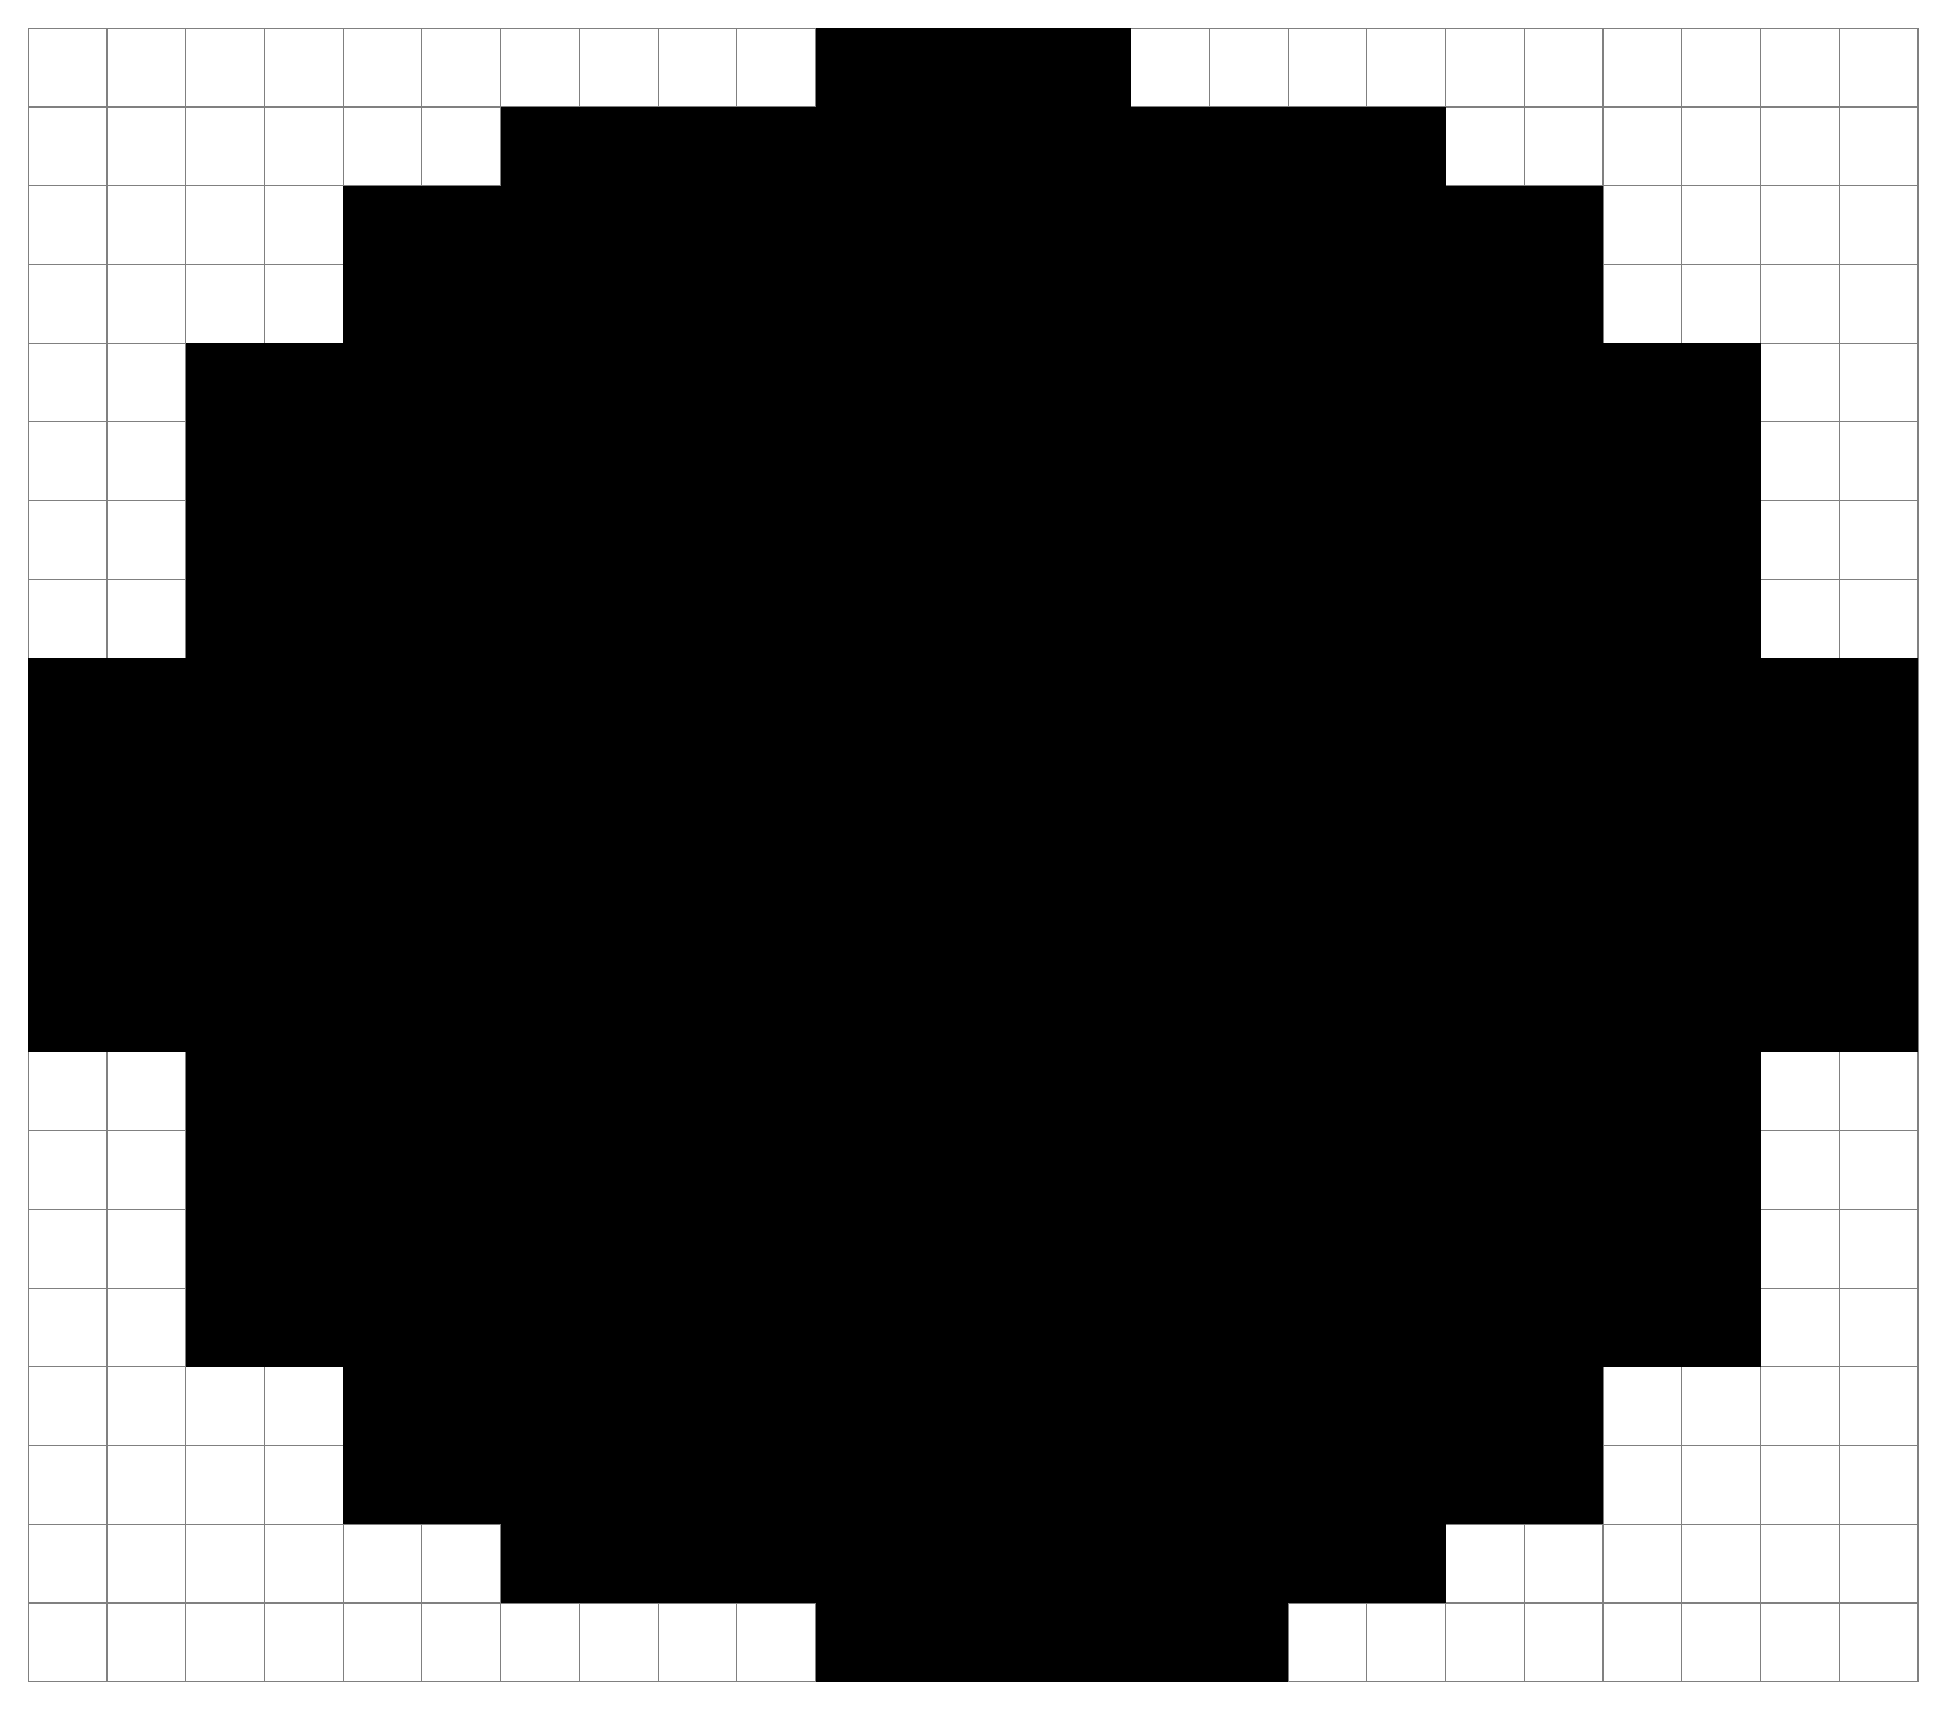
\begin{tikzpicture}

	\draw[step=1.0,gray,thin] (0,0) grid (24,21);
	\fill[\SPRITECOLOR] (10,20) rectangle ++ (1,1);
	\fill[\SPRITECOLOR] (11,20) rectangle ++ (1,1);
	\fill[\SPRITECOLOR] (12,20) rectangle ++ (1,1);
	\fill[\SPRITECOLOR] (13,20) rectangle ++ (1,1);
	\fill[\SPRITECOLOR] (6,19) rectangle ++ (1,1);
	\fill[\SPRITECOLOR] (7,19) rectangle ++ (1,1);
	\fill[\SPRITECOLOR] (8,19) rectangle ++ (1,1);
	\fill[\SPRITECOLOR] (9,19) rectangle ++ (1,1);
	\fill[\SPRITECOLOR] (10,19) rectangle ++ (1,1);
	\fill[\SPRITECOLOR] (11,19) rectangle ++ (1,1);
	\fill[\SPRITECOLOR] (12,19) rectangle ++ (1,1);
	\fill[\SPRITECOLOR] (13,19) rectangle ++ (1,1);
	\fill[\SPRITECOLOR] (14,19) rectangle ++ (1,1);
	\fill[\SPRITECOLOR] (15,19) rectangle ++ (1,1);
	\fill[\SPRITECOLOR] (16,19) rectangle ++ (1,1);
	\fill[\SPRITECOLOR] (17,19) rectangle ++ (1,1);
	\fill[\SPRITECOLOR] (4,18) rectangle ++ (1,1);
	\fill[\SPRITECOLOR] (5,18) rectangle ++ (1,1);
	\fill[\SPRITECOLOR] (6,18) rectangle ++ (1,1);
	\fill[\SPRITECOLOR] (7,18) rectangle ++ (1,1);
	\fill[\SPRITECOLOR] (8,18) rectangle ++ (1,1);
	\fill[\SPRITECOLOR] (9,18) rectangle ++ (1,1);
	\fill[\SPRITECOLOR] (10,18) rectangle ++ (1,1);
	\fill[\SPRITECOLOR] (11,18) rectangle ++ (1,1);
	\fill[\SPRITECOLOR] (12,18) rectangle ++ (1,1);
	\fill[\SPRITECOLOR] (13,18) rectangle ++ (1,1);
	\fill[\SPRITECOLOR] (14,18) rectangle ++ (1,1);
	\fill[\SPRITECOLOR] (15,18) rectangle ++ (1,1);
	\fill[\SPRITECOLOR] (16,18) rectangle ++ (1,1);
	\fill[\SPRITECOLOR] (17,18) rectangle ++ (1,1);
	\fill[\SPRITECOLOR] (18,18) rectangle ++ (1,1);
	\fill[\SPRITECOLOR] (19,18) rectangle ++ (1,1);
	\fill[\SPRITECOLOR] (4,17) rectangle ++ (1,1);
	\fill[\SPRITECOLOR] (5,17) rectangle ++ (1,1);
	\fill[\SPRITECOLOR] (6,17) rectangle ++ (1,1);
	\fill[\SPRITECOLOR] (7,17) rectangle ++ (1,1);
	\fill[\MULTICOLORTWO] (8,17) rectangle ++ (1,1);
	\fill[\MULTICOLORTWO] (9,17) rectangle ++ (1,1);
	\fill[\SPRITECOLOR] (10,17) rectangle ++ (1,1);
	\fill[\SPRITECOLOR] (11,17) rectangle ++ (1,1);
	\fill[\SPRITECOLOR] (12,17) rectangle ++ (1,1);
	\fill[\SPRITECOLOR] (13,17) rectangle ++ (1,1);
	\fill[\SPRITECOLOR] (14,17) rectangle ++ (1,1);
	\fill[\SPRITECOLOR] (15,17) rectangle ++ (1,1);
	\fill[\SPRITECOLOR] (16,17) rectangle ++ (1,1);
	\fill[\SPRITECOLOR] (17,17) rectangle ++ (1,1);
	\fill[\SPRITECOLOR] (18,17) rectangle ++ (1,1);
	\fill[\SPRITECOLOR] (19,17) rectangle ++ (1,1);
	\fill[\SPRITECOLOR] (2,16) rectangle ++ (1,1);
	\fill[\SPRITECOLOR] (3,16) rectangle ++ (1,1);
	\fill[\SPRITECOLOR] (4,16) rectangle ++ (1,1);
	\fill[\SPRITECOLOR] (5,16) rectangle ++ (1,1);
	\fill[\MULTICOLORTWO] (6,16) rectangle ++ (1,1);
	\fill[\MULTICOLORTWO] (7,16) rectangle ++ (1,1);
	\fill[\SPRITECOLOR] (8,16) rectangle ++ (1,1);
	\fill[\SPRITECOLOR] (9,16) rectangle ++ (1,1);
	\fill[\SPRITECOLOR] (10,16) rectangle ++ (1,1);
	\fill[\SPRITECOLOR] (11,16) rectangle ++ (1,1);
	\fill[\SPRITECOLOR] (12,16) rectangle ++ (1,1);
	\fill[\SPRITECOLOR] (13,16) rectangle ++ (1,1);
	\fill[\SPRITECOLOR] (14,16) rectangle ++ (1,1);
	\fill[\SPRITECOLOR] (15,16) rectangle ++ (1,1);
	\fill[\SPRITECOLOR] (16,16) rectangle ++ (1,1);
	\fill[\SPRITECOLOR] (17,16) rectangle ++ (1,1);
	\fill[\SPRITECOLOR] (18,16) rectangle ++ (1,1);
	\fill[\SPRITECOLOR] (19,16) rectangle ++ (1,1);
	\fill[\SPRITECOLOR] (20,16) rectangle ++ (1,1);
	\fill[\SPRITECOLOR] (21,16) rectangle ++ (1,1);
	\fill[\SPRITECOLOR] (2,15) rectangle ++ (1,1);
	\fill[\SPRITECOLOR] (3,15) rectangle ++ (1,1);
	\fill[\SPRITECOLOR] (4,15) rectangle ++ (1,1);
	\fill[\SPRITECOLOR] (5,15) rectangle ++ (1,1);
	\fill[\SPRITECOLOR] (6,15) rectangle ++ (1,1);
	\fill[\SPRITECOLOR] (7,15) rectangle ++ (1,1);
	\fill[\SPRITECOLOR] (8,15) rectangle ++ (1,1);
	\fill[\SPRITECOLOR] (9,15) rectangle ++ (1,1);
	\fill[\SPRITECOLOR] (10,15) rectangle ++ (1,1);
	\fill[\SPRITECOLOR] (11,15) rectangle ++ (1,1);
	\fill[\SPRITECOLOR] (12,15) rectangle ++ (1,1);
	\fill[\SPRITECOLOR] (13,15) rectangle ++ (1,1);
	\fill[\SPRITECOLOR] (14,15) rectangle ++ (1,1);
	\fill[\SPRITECOLOR] (15,15) rectangle ++ (1,1);
	\fill[\SPRITECOLOR] (16,15) rectangle ++ (1,1);
	\fill[\SPRITECOLOR] (17,15) rectangle ++ (1,1);
	\fill[\SPRITECOLOR] (18,15) rectangle ++ (1,1);
	\fill[\SPRITECOLOR] (19,15) rectangle ++ (1,1);
	\fill[\SPRITECOLOR] (20,15) rectangle ++ (1,1);
	\fill[\SPRITECOLOR] (21,15) rectangle ++ (1,1);
	\fill[\SPRITECOLOR] (2,14) rectangle ++ (1,1);
	\fill[\SPRITECOLOR] (3,14) rectangle ++ (1,1);
	\fill[\SPRITECOLOR] (4,14) rectangle ++ (1,1);
	\fill[\SPRITECOLOR] (5,14) rectangle ++ (1,1);
	\fill[\SPRITECOLOR] (6,14) rectangle ++ (1,1);
	\fill[\SPRITECOLOR] (7,14) rectangle ++ (1,1);
	\fill[\SPRITECOLOR] (8,14) rectangle ++ (1,1);
	\fill[\SPRITECOLOR] (9,14) rectangle ++ (1,1);
	\fill[\SPRITECOLOR] (10,14) rectangle ++ (1,1);
	\fill[\SPRITECOLOR] (11,14) rectangle ++ (1,1);
	\fill[\SPRITECOLOR] (12,14) rectangle ++ (1,1);
	\fill[\SPRITECOLOR] (13,14) rectangle ++ (1,1);
	\fill[\SPRITECOLOR] (14,14) rectangle ++ (1,1);
	\fill[\SPRITECOLOR] (15,14) rectangle ++ (1,1);
	\fill[\SPRITECOLOR] (16,14) rectangle ++ (1,1);
	\fill[\SPRITECOLOR] (17,14) rectangle ++ (1,1);
	\fill[\SPRITECOLOR] (18,14) rectangle ++ (1,1);
	\fill[\SPRITECOLOR] (19,14) rectangle ++ (1,1);
	\fill[\SPRITECOLOR] (20,14) rectangle ++ (1,1);
	\fill[\SPRITECOLOR] (21,14) rectangle ++ (1,1);
	\fill[\SPRITECOLOR] (2,13) rectangle ++ (1,1);
	\fill[\SPRITECOLOR] (3,13) rectangle ++ (1,1);
	\fill[\SPRITECOLOR] (4,13) rectangle ++ (1,1);
	\fill[\SPRITECOLOR] (5,13) rectangle ++ (1,1);
	\fill[\SPRITECOLOR] (6,13) rectangle ++ (1,1);
	\fill[\SPRITECOLOR] (7,13) rectangle ++ (1,1);
	\fill[\SPRITECOLOR] (8,13) rectangle ++ (1,1);
	\fill[\SPRITECOLOR] (9,13) rectangle ++ (1,1);
	\fill[\SPRITECOLOR] (10,13) rectangle ++ (1,1);
	\fill[\SPRITECOLOR] (11,13) rectangle ++ (1,1);
	\fill[\SPRITECOLOR] (12,13) rectangle ++ (1,1);
	\fill[\SPRITECOLOR] (13,13) rectangle ++ (1,1);
	\fill[\SPRITECOLOR] (14,13) rectangle ++ (1,1);
	\fill[\SPRITECOLOR] (15,13) rectangle ++ (1,1);
	\fill[\SPRITECOLOR] (16,13) rectangle ++ (1,1);
	\fill[\SPRITECOLOR] (17,13) rectangle ++ (1,1);
	\fill[\SPRITECOLOR] (18,13) rectangle ++ (1,1);
	\fill[\SPRITECOLOR] (19,13) rectangle ++ (1,1);
	\fill[\SPRITECOLOR] (20,13) rectangle ++ (1,1);
	\fill[\SPRITECOLOR] (21,13) rectangle ++ (1,1);
	\fill[\SPRITECOLOR] (0,12) rectangle ++ (1,1);
	\fill[\SPRITECOLOR] (1,12) rectangle ++ (1,1);
	\fill[\SPRITECOLOR] (2,12) rectangle ++ (1,1);
	\fill[\SPRITECOLOR] (3,12) rectangle ++ (1,1);
	\fill[\SPRITECOLOR] (4,12) rectangle ++ (1,1);
	\fill[\SPRITECOLOR] (5,12) rectangle ++ (1,1);
	\fill[\SPRITECOLOR] (6,12) rectangle ++ (1,1);
	\fill[\SPRITECOLOR] (7,12) rectangle ++ (1,1);
	\fill[\MULTICOLORTWO] (8,12) rectangle ++ (1,1);
	\fill[\MULTICOLORTWO] (9,12) rectangle ++ (1,1);
	\fill[\MULTICOLORTWO] (10,12) rectangle ++ (1,1);
	\fill[\MULTICOLORTWO] (11,12) rectangle ++ (1,1);
	\fill[\MULTICOLORTWO] (12,12) rectangle ++ (1,1);
	\fill[\MULTICOLORTWO] (13,12) rectangle ++ (1,1);
	\fill[\MULTICOLORTWO] (14,12) rectangle ++ (1,1);
	\fill[\MULTICOLORTWO] (15,12) rectangle ++ (1,1);
	\fill[\MULTICOLORTWO] (16,12) rectangle ++ (1,1);
	\fill[\MULTICOLORTWO] (17,12) rectangle ++ (1,1);
	\fill[\SPRITECOLOR] (18,12) rectangle ++ (1,1);
	\fill[\SPRITECOLOR] (19,12) rectangle ++ (1,1);
	\fill[\SPRITECOLOR] (20,12) rectangle ++ (1,1);
	\fill[\SPRITECOLOR] (21,12) rectangle ++ (1,1);
	\fill[\SPRITECOLOR] (22,12) rectangle ++ (1,1);
	\fill[\SPRITECOLOR] (23,12) rectangle ++ (1,1);
	\fill[\SPRITECOLOR] (0,11) rectangle ++ (1,1);
	\fill[\SPRITECOLOR] (1,11) rectangle ++ (1,1);
	\fill[\SPRITECOLOR] (2,11) rectangle ++ (1,1);
	\fill[\SPRITECOLOR] (3,11) rectangle ++ (1,1);
	\fill[\MULTICOLORTWO] (4,11) rectangle ++ (1,1);
	\fill[\MULTICOLORTWO] (5,11) rectangle ++ (1,1);
	\fill[\MULTICOLORTWO] (6,11) rectangle ++ (1,1);
	\fill[\MULTICOLORTWO] (7,11) rectangle ++ (1,1);
	\fill[\MULTICOLORTWO] (8,11) rectangle ++ (1,1);
	\fill[\MULTICOLORTWO] (9,11) rectangle ++ (1,1);
	\fill[\MULTICOLORONE] (10,11) rectangle ++ (1,1);
	\fill[\MULTICOLORONE] (11,11) rectangle ++ (1,1);
	\fill[\MULTICOLORONE] (12,11) rectangle ++ (1,1);
	\fill[\MULTICOLORONE] (13,11) rectangle ++ (1,1);
	\fill[\MULTICOLORONE] (14,11) rectangle ++ (1,1);
	\fill[\MULTICOLORONE] (15,11) rectangle ++ (1,1);
	\fill[\MULTICOLORTWO] (16,11) rectangle ++ (1,1);
	\fill[\MULTICOLORTWO] (17,11) rectangle ++ (1,1);
	\fill[\MULTICOLORTWO] (18,11) rectangle ++ (1,1);
	\fill[\MULTICOLORTWO] (19,11) rectangle ++ (1,1);
	\fill[\SPRITECOLOR] (20,11) rectangle ++ (1,1);
	\fill[\SPRITECOLOR] (21,11) rectangle ++ (1,1);
	\fill[\SPRITECOLOR] (22,11) rectangle ++ (1,1);
	\fill[\SPRITECOLOR] (23,11) rectangle ++ (1,1);
	\fill[\SPRITECOLOR] (0,10) rectangle ++ (1,1);
	\fill[\SPRITECOLOR] (1,10) rectangle ++ (1,1);
	\fill[\SPRITECOLOR] (2,10) rectangle ++ (1,1);
	\fill[\SPRITECOLOR] (3,10) rectangle ++ (1,1);
	\fill[\MULTICOLORTWO] (4,10) rectangle ++ (1,1);
	\fill[\MULTICOLORTWO] (5,10) rectangle ++ (1,1);
	\fill[\MULTICOLORTWO] (6,10) rectangle ++ (1,1);
	\fill[\MULTICOLORTWO] (7,10) rectangle ++ (1,1);
	\fill[\MULTICOLORTWO] (8,10) rectangle ++ (1,1);
	\fill[\MULTICOLORTWO] (9,10) rectangle ++ (1,1);
	\fill[\MULTICOLORONE] (10,10) rectangle ++ (1,1);
	\fill[\MULTICOLORONE] (11,10) rectangle ++ (1,1);
	\fill[\MULTICOLORONE] (12,10) rectangle ++ (1,1);
	\fill[\MULTICOLORONE] (13,10) rectangle ++ (1,1);
	\fill[\MULTICOLORONE] (14,10) rectangle ++ (1,1);
	\fill[\MULTICOLORONE] (15,10) rectangle ++ (1,1);
	\fill[\MULTICOLORTWO] (16,10) rectangle ++ (1,1);
	\fill[\MULTICOLORTWO] (17,10) rectangle ++ (1,1);
	\fill[\MULTICOLORTWO] (18,10) rectangle ++ (1,1);
	\fill[\MULTICOLORTWO] (19,10) rectangle ++ (1,1);
	\fill[\MULTICOLORTWO] (20,10) rectangle ++ (1,1);
	\fill[\MULTICOLORTWO] (21,10) rectangle ++ (1,1);
	\fill[\SPRITECOLOR] (22,10) rectangle ++ (1,1);
	\fill[\SPRITECOLOR] (23,10) rectangle ++ (1,1);
	\fill[\SPRITECOLOR] (0,9) rectangle ++ (1,1);
	\fill[\SPRITECOLOR] (1,9) rectangle ++ (1,1);
	\fill[\SPRITECOLOR] (2,9) rectangle ++ (1,1);
	\fill[\SPRITECOLOR] (3,9) rectangle ++ (1,1);
	\fill[\SPRITECOLOR] (4,9) rectangle ++ (1,1);
	\fill[\SPRITECOLOR] (5,9) rectangle ++ (1,1);
	\fill[\MULTICOLORTWO] (6,9) rectangle ++ (1,1);
	\fill[\MULTICOLORTWO] (7,9) rectangle ++ (1,1);
	\fill[\MULTICOLORTWO] (8,9) rectangle ++ (1,1);
	\fill[\MULTICOLORTWO] (9,9) rectangle ++ (1,1);
	\fill[\MULTICOLORONE] (10,9) rectangle ++ (1,1);
	\fill[\MULTICOLORONE] (11,9) rectangle ++ (1,1);
	\fill[\MULTICOLORONE] (12,9) rectangle ++ (1,1);
	\fill[\MULTICOLORONE] (13,9) rectangle ++ (1,1);
	\fill[\MULTICOLORONE] (14,9) rectangle ++ (1,1);
	\fill[\MULTICOLORONE] (15,9) rectangle ++ (1,1);
	\fill[\MULTICOLORTWO] (16,9) rectangle ++ (1,1);
	\fill[\MULTICOLORTWO] (17,9) rectangle ++ (1,1);
	\fill[\MULTICOLORTWO] (18,9) rectangle ++ (1,1);
	\fill[\MULTICOLORTWO] (19,9) rectangle ++ (1,1);
	\fill[\MULTICOLORTWO] (20,9) rectangle ++ (1,1);
	\fill[\MULTICOLORTWO] (21,9) rectangle ++ (1,1);
	\fill[\SPRITECOLOR] (22,9) rectangle ++ (1,1);
	\fill[\SPRITECOLOR] (23,9) rectangle ++ (1,1);
	\fill[\SPRITECOLOR] (0,8) rectangle ++ (1,1);
	\fill[\SPRITECOLOR] (1,8) rectangle ++ (1,1);
	\fill[\SPRITECOLOR] (2,8) rectangle ++ (1,1);
	\fill[\SPRITECOLOR] (3,8) rectangle ++ (1,1);
	\fill[\SPRITECOLOR] (4,8) rectangle ++ (1,1);
	\fill[\SPRITECOLOR] (5,8) rectangle ++ (1,1);
	\fill[\SPRITECOLOR] (6,8) rectangle ++ (1,1);
	\fill[\SPRITECOLOR] (7,8) rectangle ++ (1,1);
	\fill[\MULTICOLORTWO] (8,8) rectangle ++ (1,1);
	\fill[\MULTICOLORTWO] (9,8) rectangle ++ (1,1);
	\fill[\MULTICOLORTWO] (10,8) rectangle ++ (1,1);
	\fill[\MULTICOLORTWO] (11,8) rectangle ++ (1,1);
	\fill[\MULTICOLORTWO] (12,8) rectangle ++ (1,1);
	\fill[\MULTICOLORTWO] (13,8) rectangle ++ (1,1);
	\fill[\MULTICOLORTWO] (14,8) rectangle ++ (1,1);
	\fill[\MULTICOLORTWO] (15,8) rectangle ++ (1,1);
	\fill[\MULTICOLORTWO] (16,8) rectangle ++ (1,1);
	\fill[\MULTICOLORTWO] (17,8) rectangle ++ (1,1);
	\fill[\SPRITECOLOR] (18,8) rectangle ++ (1,1);
	\fill[\SPRITECOLOR] (19,8) rectangle ++ (1,1);
	\fill[\SPRITECOLOR] (20,8) rectangle ++ (1,1);
	\fill[\SPRITECOLOR] (21,8) rectangle ++ (1,1);
	\fill[\SPRITECOLOR] (22,8) rectangle ++ (1,1);
	\fill[\SPRITECOLOR] (23,8) rectangle ++ (1,1);
	\fill[\SPRITECOLOR] (2,7) rectangle ++ (1,1);
	\fill[\SPRITECOLOR] (3,7) rectangle ++ (1,1);
	\fill[\SPRITECOLOR] (4,7) rectangle ++ (1,1);
	\fill[\SPRITECOLOR] (5,7) rectangle ++ (1,1);
	\fill[\SPRITECOLOR] (6,7) rectangle ++ (1,1);
	\fill[\SPRITECOLOR] (7,7) rectangle ++ (1,1);
	\fill[\SPRITECOLOR] (8,7) rectangle ++ (1,1);
	\fill[\SPRITECOLOR] (9,7) rectangle ++ (1,1);
	\fill[\SPRITECOLOR] (10,7) rectangle ++ (1,1);
	\fill[\SPRITECOLOR] (11,7) rectangle ++ (1,1);
	\fill[\SPRITECOLOR] (12,7) rectangle ++ (1,1);
	\fill[\SPRITECOLOR] (13,7) rectangle ++ (1,1);
	\fill[\SPRITECOLOR] (14,7) rectangle ++ (1,1);
	\fill[\SPRITECOLOR] (15,7) rectangle ++ (1,1);
	\fill[\SPRITECOLOR] (16,7) rectangle ++ (1,1);
	\fill[\SPRITECOLOR] (17,7) rectangle ++ (1,1);
	\fill[\SPRITECOLOR] (18,7) rectangle ++ (1,1);
	\fill[\SPRITECOLOR] (19,7) rectangle ++ (1,1);
	\fill[\SPRITECOLOR] (20,7) rectangle ++ (1,1);
	\fill[\SPRITECOLOR] (21,7) rectangle ++ (1,1);
	\fill[\SPRITECOLOR] (2,6) rectangle ++ (1,1);
	\fill[\SPRITECOLOR] (3,6) rectangle ++ (1,1);
	\fill[\SPRITECOLOR] (4,6) rectangle ++ (1,1);
	\fill[\SPRITECOLOR] (5,6) rectangle ++ (1,1);
	\fill[\SPRITECOLOR] (6,6) rectangle ++ (1,1);
	\fill[\SPRITECOLOR] (7,6) rectangle ++ (1,1);
	\fill[\SPRITECOLOR] (8,6) rectangle ++ (1,1);
	\fill[\SPRITECOLOR] (9,6) rectangle ++ (1,1);
	\fill[\SPRITECOLOR] (10,6) rectangle ++ (1,1);
	\fill[\SPRITECOLOR] (11,6) rectangle ++ (1,1);
	\fill[\SPRITECOLOR] (12,6) rectangle ++ (1,1);
	\fill[\SPRITECOLOR] (13,6) rectangle ++ (1,1);
	\fill[\SPRITECOLOR] (14,6) rectangle ++ (1,1);
	\fill[\SPRITECOLOR] (15,6) rectangle ++ (1,1);
	\fill[\SPRITECOLOR] (16,6) rectangle ++ (1,1);
	\fill[\SPRITECOLOR] (17,6) rectangle ++ (1,1);
	\fill[\SPRITECOLOR] (18,6) rectangle ++ (1,1);
	\fill[\SPRITECOLOR] (19,6) rectangle ++ (1,1);
	\fill[\SPRITECOLOR] (20,6) rectangle ++ (1,1);
	\fill[\SPRITECOLOR] (21,6) rectangle ++ (1,1);
	\fill[\SPRITECOLOR] (2,5) rectangle ++ (1,1);
	\fill[\SPRITECOLOR] (3,5) rectangle ++ (1,1);
	\fill[\SPRITECOLOR] (4,5) rectangle ++ (1,1);
	\fill[\SPRITECOLOR] (5,5) rectangle ++ (1,1);
	\fill[\SPRITECOLOR] (6,5) rectangle ++ (1,1);
	\fill[\SPRITECOLOR] (7,5) rectangle ++ (1,1);
	\fill[\SPRITECOLOR] (8,5) rectangle ++ (1,1);
	\fill[\SPRITECOLOR] (9,5) rectangle ++ (1,1);
	\fill[\SPRITECOLOR] (10,5) rectangle ++ (1,1);
	\fill[\SPRITECOLOR] (11,5) rectangle ++ (1,1);
	\fill[\SPRITECOLOR] (12,5) rectangle ++ (1,1);
	\fill[\SPRITECOLOR] (13,5) rectangle ++ (1,1);
	\fill[\SPRITECOLOR] (14,5) rectangle ++ (1,1);
	\fill[\SPRITECOLOR] (15,5) rectangle ++ (1,1);
	\fill[\SPRITECOLOR] (16,5) rectangle ++ (1,1);
	\fill[\SPRITECOLOR] (17,5) rectangle ++ (1,1);
	\fill[\SPRITECOLOR] (18,5) rectangle ++ (1,1);
	\fill[\SPRITECOLOR] (19,5) rectangle ++ (1,1);
	\fill[\SPRITECOLOR] (20,5) rectangle ++ (1,1);
	\fill[\SPRITECOLOR] (21,5) rectangle ++ (1,1);
	\fill[\SPRITECOLOR] (2,4) rectangle ++ (1,1);
	\fill[\SPRITECOLOR] (3,4) rectangle ++ (1,1);
	\fill[\SPRITECOLOR] (4,4) rectangle ++ (1,1);
	\fill[\SPRITECOLOR] (5,4) rectangle ++ (1,1);
	\fill[\SPRITECOLOR] (6,4) rectangle ++ (1,1);
	\fill[\SPRITECOLOR] (7,4) rectangle ++ (1,1);
	\fill[\SPRITECOLOR] (8,4) rectangle ++ (1,1);
	\fill[\SPRITECOLOR] (9,4) rectangle ++ (1,1);
	\fill[\SPRITECOLOR] (10,4) rectangle ++ (1,1);
	\fill[\SPRITECOLOR] (11,4) rectangle ++ (1,1);
	\fill[\SPRITECOLOR] (12,4) rectangle ++ (1,1);
	\fill[\SPRITECOLOR] (13,4) rectangle ++ (1,1);
	\fill[\SPRITECOLOR] (14,4) rectangle ++ (1,1);
	\fill[\SPRITECOLOR] (15,4) rectangle ++ (1,1);
	\fill[\SPRITECOLOR] (16,4) rectangle ++ (1,1);
	\fill[\SPRITECOLOR] (17,4) rectangle ++ (1,1);
	\fill[\SPRITECOLOR] (18,4) rectangle ++ (1,1);
	\fill[\SPRITECOLOR] (19,4) rectangle ++ (1,1);
	\fill[\SPRITECOLOR] (20,4) rectangle ++ (1,1);
	\fill[\SPRITECOLOR] (21,4) rectangle ++ (1,1);
	\fill[\SPRITECOLOR] (4,3) rectangle ++ (1,1);
	\fill[\SPRITECOLOR] (5,3) rectangle ++ (1,1);
	\fill[\SPRITECOLOR] (6,3) rectangle ++ (1,1);
	\fill[\SPRITECOLOR] (7,3) rectangle ++ (1,1);
	\fill[\SPRITECOLOR] (8,3) rectangle ++ (1,1);
	\fill[\SPRITECOLOR] (9,3) rectangle ++ (1,1);
	\fill[\SPRITECOLOR] (10,3) rectangle ++ (1,1);
	\fill[\SPRITECOLOR] (11,3) rectangle ++ (1,1);
	\fill[\SPRITECOLOR] (12,3) rectangle ++ (1,1);
	\fill[\SPRITECOLOR] (13,3) rectangle ++ (1,1);
	\fill[\SPRITECOLOR] (14,3) rectangle ++ (1,1);
	\fill[\SPRITECOLOR] (15,3) rectangle ++ (1,1);
	\fill[\SPRITECOLOR] (16,3) rectangle ++ (1,1);
	\fill[\SPRITECOLOR] (17,3) rectangle ++ (1,1);
	\fill[\SPRITECOLOR] (18,3) rectangle ++ (1,1);
	\fill[\SPRITECOLOR] (19,3) rectangle ++ (1,1);
	\fill[\SPRITECOLOR] (4,2) rectangle ++ (1,1);
	\fill[\SPRITECOLOR] (5,2) rectangle ++ (1,1);
	\fill[\SPRITECOLOR] (6,2) rectangle ++ (1,1);
	\fill[\SPRITECOLOR] (7,2) rectangle ++ (1,1);
	\fill[\SPRITECOLOR] (8,2) rectangle ++ (1,1);
	\fill[\SPRITECOLOR] (9,2) rectangle ++ (1,1);
	\fill[\SPRITECOLOR] (10,2) rectangle ++ (1,1);
	\fill[\SPRITECOLOR] (11,2) rectangle ++ (1,1);
	\fill[\SPRITECOLOR] (12,2) rectangle ++ (1,1);
	\fill[\SPRITECOLOR] (13,2) rectangle ++ (1,1);
	\fill[\SPRITECOLOR] (14,2) rectangle ++ (1,1);
	\fill[\SPRITECOLOR] (15,2) rectangle ++ (1,1);
	\fill[\SPRITECOLOR] (16,2) rectangle ++ (1,1);
	\fill[\SPRITECOLOR] (17,2) rectangle ++ (1,1);
	\fill[\SPRITECOLOR] (18,2) rectangle ++ (1,1);
	\fill[\SPRITECOLOR] (19,2) rectangle ++ (1,1);
	\fill[\SPRITECOLOR] (6,1) rectangle ++ (1,1);
	\fill[\SPRITECOLOR] (7,1) rectangle ++ (1,1);
	\fill[\SPRITECOLOR] (8,1) rectangle ++ (1,1);
	\fill[\SPRITECOLOR] (9,1) rectangle ++ (1,1);
	\fill[\SPRITECOLOR] (10,1) rectangle ++ (1,1);
	\fill[\SPRITECOLOR] (11,1) rectangle ++ (1,1);
	\fill[\SPRITECOLOR] (12,1) rectangle ++ (1,1);
	\fill[\SPRITECOLOR] (13,1) rectangle ++ (1,1);
	\fill[\SPRITECOLOR] (14,1) rectangle ++ (1,1);
	\fill[\SPRITECOLOR] (15,1) rectangle ++ (1,1);
	\fill[\SPRITECOLOR] (16,1) rectangle ++ (1,1);
	\fill[\SPRITECOLOR] (17,1) rectangle ++ (1,1);
	\fill[\SPRITECOLOR] (10,0) rectangle ++ (1,1);
	\fill[\SPRITECOLOR] (11,0) rectangle ++ (1,1);
	\fill[\SPRITECOLOR] (12,0) rectangle ++ (1,1);
	\fill[\SPRITECOLOR] (13,0) rectangle ++ (1,1);
	\fill[\SPRITECOLOR] (14,0) rectangle ++ (1,1);
	\fill[\SPRITECOLOR] (15,0) rectangle ++ (1,1);

      \end{tikzpicture}
    \end{adjustbox}
  }\caption{BONUS\_IBALL2}
\end{figure}

	\end{subfigure}
} & 
\makecell[l]{
	\begin{subfigure}{0.3\textwidth}
    \def\MULTICOLORONE{gray}
    \def\MULTICOLORTWO{white}
    \def\SPRITECOLOR{black}
		
\begin{figure}[H]
  {
    \setlength{\tabcolsep}{3.0pt}
    \setlength\cmidrulewidth{\heavyrulewidth} % Make cmidrule = 
    \begin{adjustbox}{width=3cm,center}
      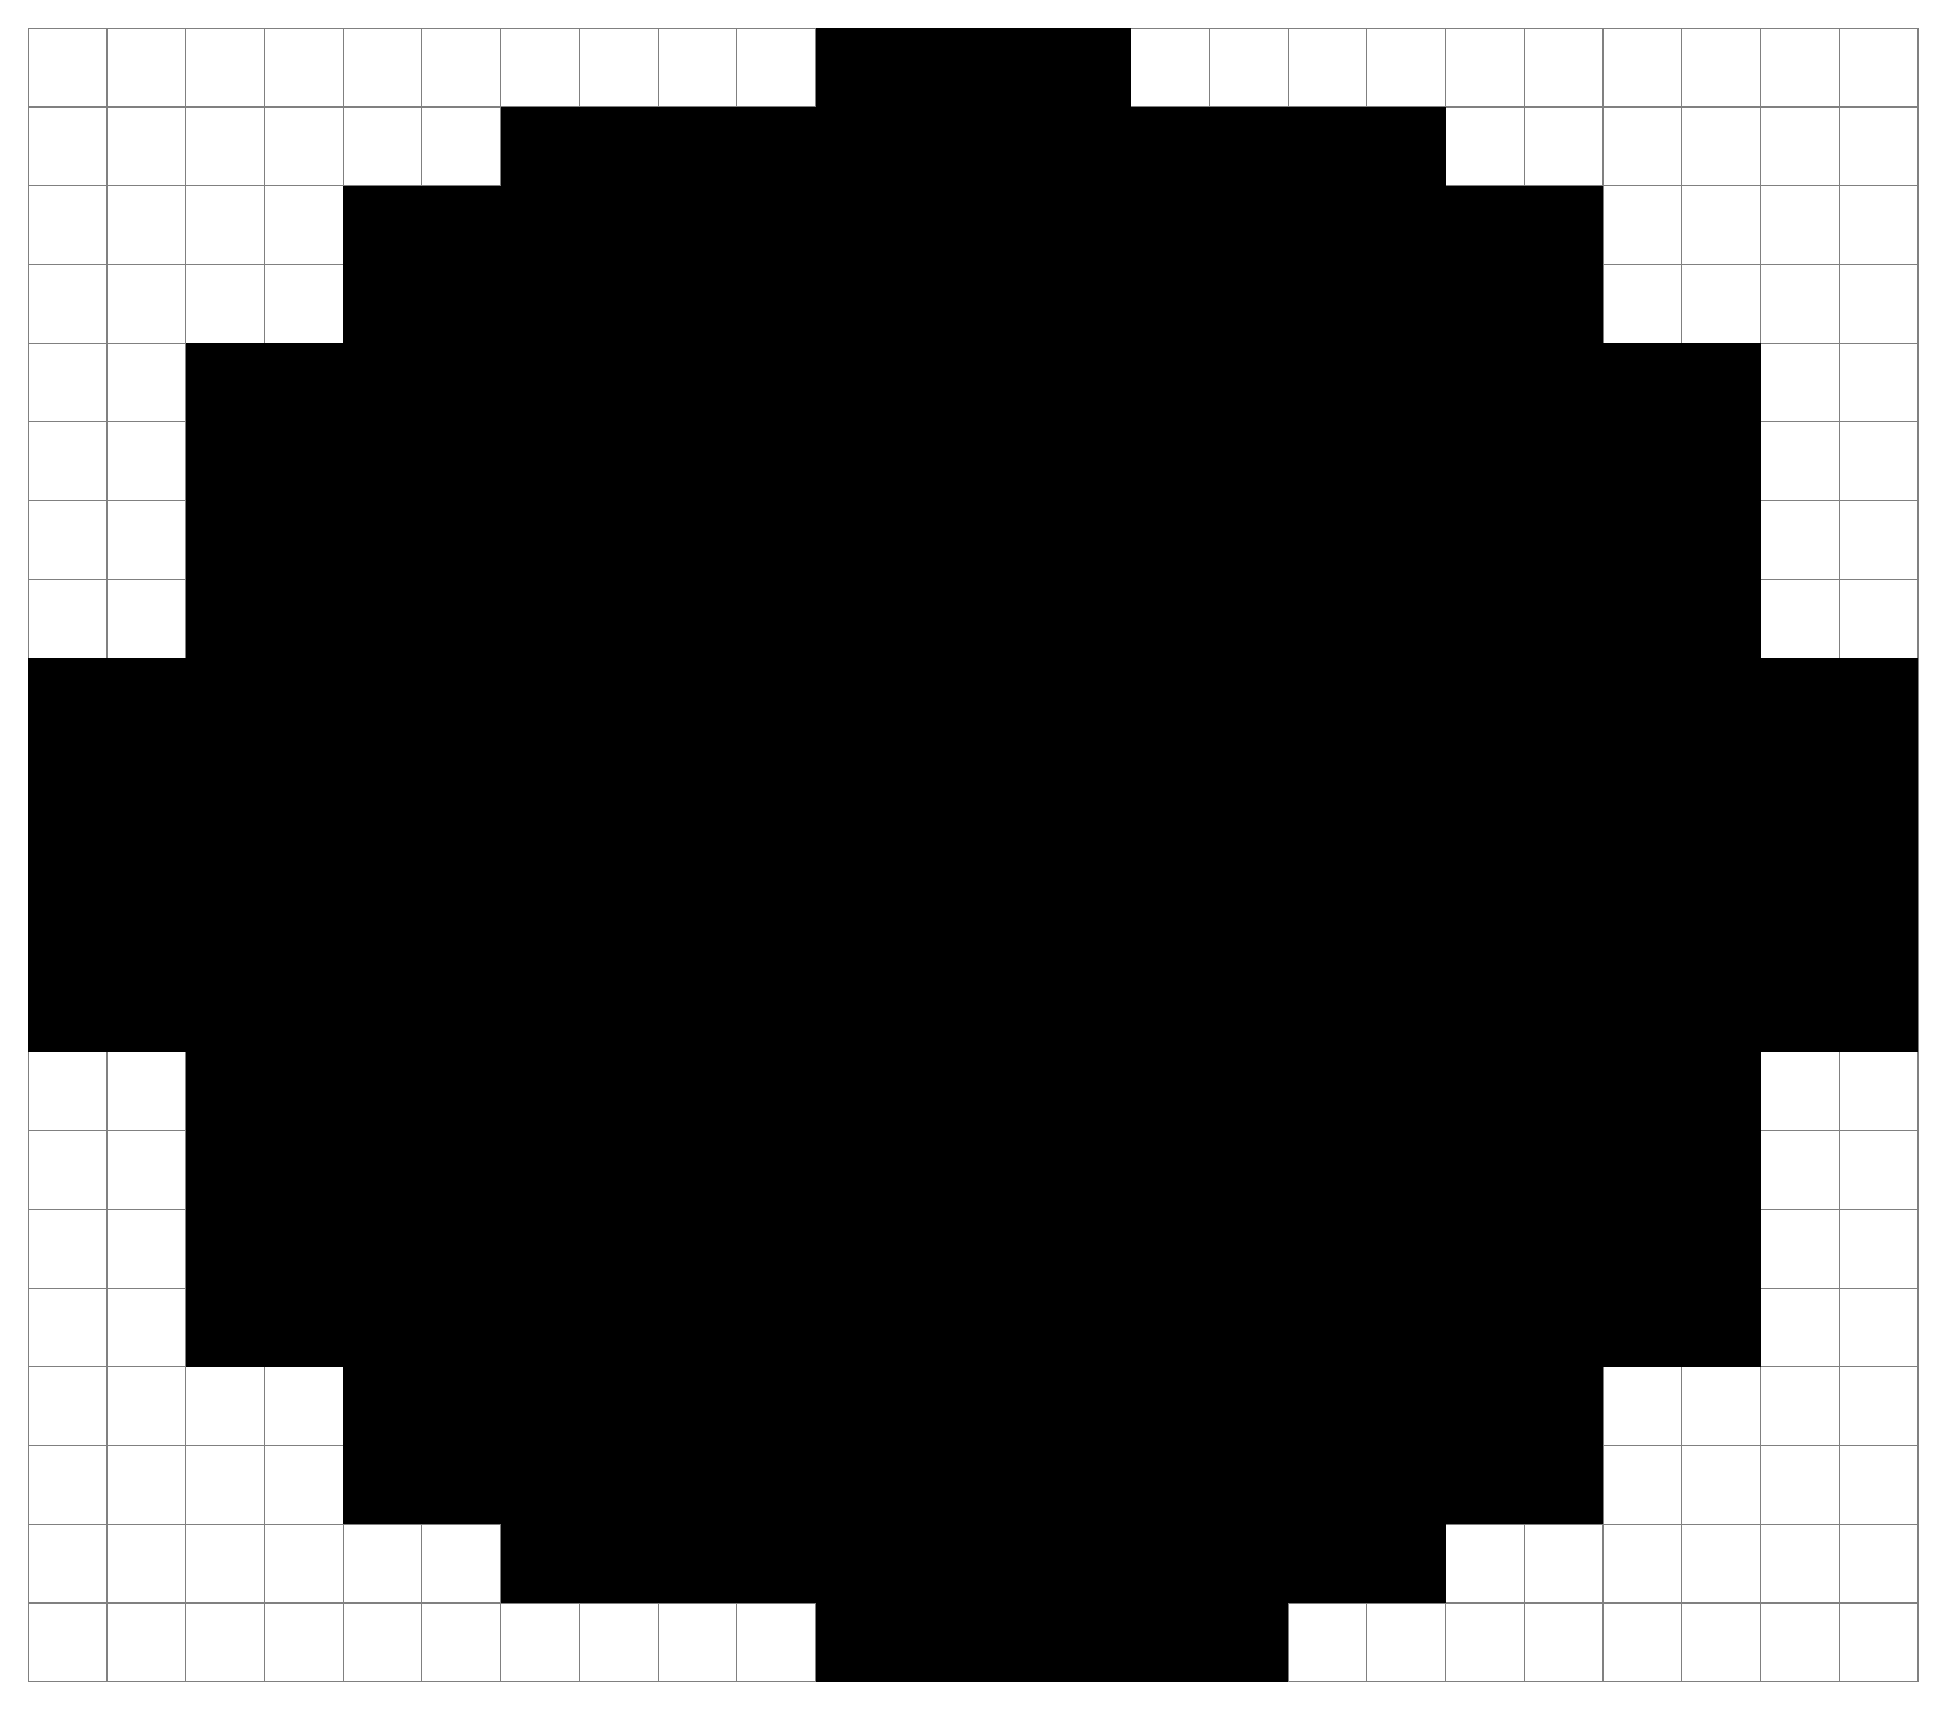
\begin{tikzpicture}

	\draw[step=1.0,gray,thin] (0,0) grid (24,21);
	\fill[\SPRITECOLOR] (10,20) rectangle ++ (1,1);
	\fill[\SPRITECOLOR] (11,20) rectangle ++ (1,1);
	\fill[\SPRITECOLOR] (12,20) rectangle ++ (1,1);
	\fill[\SPRITECOLOR] (13,20) rectangle ++ (1,1);
	\fill[\SPRITECOLOR] (6,19) rectangle ++ (1,1);
	\fill[\SPRITECOLOR] (7,19) rectangle ++ (1,1);
	\fill[\SPRITECOLOR] (8,19) rectangle ++ (1,1);
	\fill[\SPRITECOLOR] (9,19) rectangle ++ (1,1);
	\fill[\SPRITECOLOR] (10,19) rectangle ++ (1,1);
	\fill[\SPRITECOLOR] (11,19) rectangle ++ (1,1);
	\fill[\SPRITECOLOR] (12,19) rectangle ++ (1,1);
	\fill[\SPRITECOLOR] (13,19) rectangle ++ (1,1);
	\fill[\SPRITECOLOR] (14,19) rectangle ++ (1,1);
	\fill[\SPRITECOLOR] (15,19) rectangle ++ (1,1);
	\fill[\SPRITECOLOR] (16,19) rectangle ++ (1,1);
	\fill[\SPRITECOLOR] (17,19) rectangle ++ (1,1);
	\fill[\SPRITECOLOR] (4,18) rectangle ++ (1,1);
	\fill[\SPRITECOLOR] (5,18) rectangle ++ (1,1);
	\fill[\SPRITECOLOR] (6,18) rectangle ++ (1,1);
	\fill[\SPRITECOLOR] (7,18) rectangle ++ (1,1);
	\fill[\SPRITECOLOR] (8,18) rectangle ++ (1,1);
	\fill[\SPRITECOLOR] (9,18) rectangle ++ (1,1);
	\fill[\SPRITECOLOR] (10,18) rectangle ++ (1,1);
	\fill[\SPRITECOLOR] (11,18) rectangle ++ (1,1);
	\fill[\SPRITECOLOR] (12,18) rectangle ++ (1,1);
	\fill[\SPRITECOLOR] (13,18) rectangle ++ (1,1);
	\fill[\SPRITECOLOR] (14,18) rectangle ++ (1,1);
	\fill[\SPRITECOLOR] (15,18) rectangle ++ (1,1);
	\fill[\SPRITECOLOR] (16,18) rectangle ++ (1,1);
	\fill[\SPRITECOLOR] (17,18) rectangle ++ (1,1);
	\fill[\SPRITECOLOR] (18,18) rectangle ++ (1,1);
	\fill[\SPRITECOLOR] (19,18) rectangle ++ (1,1);
	\fill[\SPRITECOLOR] (4,17) rectangle ++ (1,1);
	\fill[\SPRITECOLOR] (5,17) rectangle ++ (1,1);
	\fill[\SPRITECOLOR] (6,17) rectangle ++ (1,1);
	\fill[\SPRITECOLOR] (7,17) rectangle ++ (1,1);
	\fill[\MULTICOLORTWO] (8,17) rectangle ++ (1,1);
	\fill[\MULTICOLORTWO] (9,17) rectangle ++ (1,1);
	\fill[\SPRITECOLOR] (10,17) rectangle ++ (1,1);
	\fill[\SPRITECOLOR] (11,17) rectangle ++ (1,1);
	\fill[\SPRITECOLOR] (12,17) rectangle ++ (1,1);
	\fill[\SPRITECOLOR] (13,17) rectangle ++ (1,1);
	\fill[\SPRITECOLOR] (14,17) rectangle ++ (1,1);
	\fill[\SPRITECOLOR] (15,17) rectangle ++ (1,1);
	\fill[\SPRITECOLOR] (16,17) rectangle ++ (1,1);
	\fill[\SPRITECOLOR] (17,17) rectangle ++ (1,1);
	\fill[\SPRITECOLOR] (18,17) rectangle ++ (1,1);
	\fill[\SPRITECOLOR] (19,17) rectangle ++ (1,1);
	\fill[\SPRITECOLOR] (2,16) rectangle ++ (1,1);
	\fill[\SPRITECOLOR] (3,16) rectangle ++ (1,1);
	\fill[\SPRITECOLOR] (4,16) rectangle ++ (1,1);
	\fill[\SPRITECOLOR] (5,16) rectangle ++ (1,1);
	\fill[\MULTICOLORTWO] (6,16) rectangle ++ (1,1);
	\fill[\MULTICOLORTWO] (7,16) rectangle ++ (1,1);
	\fill[\SPRITECOLOR] (8,16) rectangle ++ (1,1);
	\fill[\SPRITECOLOR] (9,16) rectangle ++ (1,1);
	\fill[\SPRITECOLOR] (10,16) rectangle ++ (1,1);
	\fill[\SPRITECOLOR] (11,16) rectangle ++ (1,1);
	\fill[\SPRITECOLOR] (12,16) rectangle ++ (1,1);
	\fill[\SPRITECOLOR] (13,16) rectangle ++ (1,1);
	\fill[\SPRITECOLOR] (14,16) rectangle ++ (1,1);
	\fill[\SPRITECOLOR] (15,16) rectangle ++ (1,1);
	\fill[\SPRITECOLOR] (16,16) rectangle ++ (1,1);
	\fill[\SPRITECOLOR] (17,16) rectangle ++ (1,1);
	\fill[\SPRITECOLOR] (18,16) rectangle ++ (1,1);
	\fill[\SPRITECOLOR] (19,16) rectangle ++ (1,1);
	\fill[\SPRITECOLOR] (20,16) rectangle ++ (1,1);
	\fill[\SPRITECOLOR] (21,16) rectangle ++ (1,1);
	\fill[\SPRITECOLOR] (2,15) rectangle ++ (1,1);
	\fill[\SPRITECOLOR] (3,15) rectangle ++ (1,1);
	\fill[\SPRITECOLOR] (4,15) rectangle ++ (1,1);
	\fill[\SPRITECOLOR] (5,15) rectangle ++ (1,1);
	\fill[\SPRITECOLOR] (6,15) rectangle ++ (1,1);
	\fill[\SPRITECOLOR] (7,15) rectangle ++ (1,1);
	\fill[\SPRITECOLOR] (8,15) rectangle ++ (1,1);
	\fill[\SPRITECOLOR] (9,15) rectangle ++ (1,1);
	\fill[\SPRITECOLOR] (10,15) rectangle ++ (1,1);
	\fill[\SPRITECOLOR] (11,15) rectangle ++ (1,1);
	\fill[\SPRITECOLOR] (12,15) rectangle ++ (1,1);
	\fill[\SPRITECOLOR] (13,15) rectangle ++ (1,1);
	\fill[\SPRITECOLOR] (14,15) rectangle ++ (1,1);
	\fill[\SPRITECOLOR] (15,15) rectangle ++ (1,1);
	\fill[\SPRITECOLOR] (16,15) rectangle ++ (1,1);
	\fill[\SPRITECOLOR] (17,15) rectangle ++ (1,1);
	\fill[\SPRITECOLOR] (18,15) rectangle ++ (1,1);
	\fill[\SPRITECOLOR] (19,15) rectangle ++ (1,1);
	\fill[\SPRITECOLOR] (20,15) rectangle ++ (1,1);
	\fill[\SPRITECOLOR] (21,15) rectangle ++ (1,1);
	\fill[\SPRITECOLOR] (2,14) rectangle ++ (1,1);
	\fill[\SPRITECOLOR] (3,14) rectangle ++ (1,1);
	\fill[\SPRITECOLOR] (4,14) rectangle ++ (1,1);
	\fill[\SPRITECOLOR] (5,14) rectangle ++ (1,1);
	\fill[\SPRITECOLOR] (6,14) rectangle ++ (1,1);
	\fill[\SPRITECOLOR] (7,14) rectangle ++ (1,1);
	\fill[\SPRITECOLOR] (8,14) rectangle ++ (1,1);
	\fill[\SPRITECOLOR] (9,14) rectangle ++ (1,1);
	\fill[\SPRITECOLOR] (10,14) rectangle ++ (1,1);
	\fill[\SPRITECOLOR] (11,14) rectangle ++ (1,1);
	\fill[\SPRITECOLOR] (12,14) rectangle ++ (1,1);
	\fill[\SPRITECOLOR] (13,14) rectangle ++ (1,1);
	\fill[\SPRITECOLOR] (14,14) rectangle ++ (1,1);
	\fill[\SPRITECOLOR] (15,14) rectangle ++ (1,1);
	\fill[\SPRITECOLOR] (16,14) rectangle ++ (1,1);
	\fill[\SPRITECOLOR] (17,14) rectangle ++ (1,1);
	\fill[\SPRITECOLOR] (18,14) rectangle ++ (1,1);
	\fill[\SPRITECOLOR] (19,14) rectangle ++ (1,1);
	\fill[\SPRITECOLOR] (20,14) rectangle ++ (1,1);
	\fill[\SPRITECOLOR] (21,14) rectangle ++ (1,1);
	\fill[\SPRITECOLOR] (2,13) rectangle ++ (1,1);
	\fill[\SPRITECOLOR] (3,13) rectangle ++ (1,1);
	\fill[\SPRITECOLOR] (4,13) rectangle ++ (1,1);
	\fill[\SPRITECOLOR] (5,13) rectangle ++ (1,1);
	\fill[\SPRITECOLOR] (6,13) rectangle ++ (1,1);
	\fill[\SPRITECOLOR] (7,13) rectangle ++ (1,1);
	\fill[\SPRITECOLOR] (8,13) rectangle ++ (1,1);
	\fill[\SPRITECOLOR] (9,13) rectangle ++ (1,1);
	\fill[\SPRITECOLOR] (10,13) rectangle ++ (1,1);
	\fill[\SPRITECOLOR] (11,13) rectangle ++ (1,1);
	\fill[\SPRITECOLOR] (12,13) rectangle ++ (1,1);
	\fill[\SPRITECOLOR] (13,13) rectangle ++ (1,1);
	\fill[\SPRITECOLOR] (14,13) rectangle ++ (1,1);
	\fill[\SPRITECOLOR] (15,13) rectangle ++ (1,1);
	\fill[\SPRITECOLOR] (16,13) rectangle ++ (1,1);
	\fill[\SPRITECOLOR] (17,13) rectangle ++ (1,1);
	\fill[\SPRITECOLOR] (18,13) rectangle ++ (1,1);
	\fill[\SPRITECOLOR] (19,13) rectangle ++ (1,1);
	\fill[\SPRITECOLOR] (20,13) rectangle ++ (1,1);
	\fill[\SPRITECOLOR] (21,13) rectangle ++ (1,1);
	\fill[\SPRITECOLOR] (0,12) rectangle ++ (1,1);
	\fill[\SPRITECOLOR] (1,12) rectangle ++ (1,1);
	\fill[\SPRITECOLOR] (2,12) rectangle ++ (1,1);
	\fill[\SPRITECOLOR] (3,12) rectangle ++ (1,1);
	\fill[\SPRITECOLOR] (4,12) rectangle ++ (1,1);
	\fill[\SPRITECOLOR] (5,12) rectangle ++ (1,1);
	\fill[\SPRITECOLOR] (6,12) rectangle ++ (1,1);
	\fill[\SPRITECOLOR] (7,12) rectangle ++ (1,1);
	\fill[\SPRITECOLOR] (8,12) rectangle ++ (1,1);
	\fill[\SPRITECOLOR] (9,12) rectangle ++ (1,1);
	\fill[\SPRITECOLOR] (10,12) rectangle ++ (1,1);
	\fill[\SPRITECOLOR] (11,12) rectangle ++ (1,1);
	\fill[\SPRITECOLOR] (12,12) rectangle ++ (1,1);
	\fill[\SPRITECOLOR] (13,12) rectangle ++ (1,1);
	\fill[\SPRITECOLOR] (14,12) rectangle ++ (1,1);
	\fill[\SPRITECOLOR] (15,12) rectangle ++ (1,1);
	\fill[\SPRITECOLOR] (16,12) rectangle ++ (1,1);
	\fill[\SPRITECOLOR] (17,12) rectangle ++ (1,1);
	\fill[\SPRITECOLOR] (18,12) rectangle ++ (1,1);
	\fill[\SPRITECOLOR] (19,12) rectangle ++ (1,1);
	\fill[\SPRITECOLOR] (20,12) rectangle ++ (1,1);
	\fill[\SPRITECOLOR] (21,12) rectangle ++ (1,1);
	\fill[\SPRITECOLOR] (22,12) rectangle ++ (1,1);
	\fill[\SPRITECOLOR] (23,12) rectangle ++ (1,1);
	\fill[\SPRITECOLOR] (0,11) rectangle ++ (1,1);
	\fill[\SPRITECOLOR] (1,11) rectangle ++ (1,1);
	\fill[\SPRITECOLOR] (2,11) rectangle ++ (1,1);
	\fill[\SPRITECOLOR] (3,11) rectangle ++ (1,1);
	\fill[\SPRITECOLOR] (4,11) rectangle ++ (1,1);
	\fill[\SPRITECOLOR] (5,11) rectangle ++ (1,1);
	\fill[\SPRITECOLOR] (6,11) rectangle ++ (1,1);
	\fill[\SPRITECOLOR] (7,11) rectangle ++ (1,1);
	\fill[\SPRITECOLOR] (8,11) rectangle ++ (1,1);
	\fill[\SPRITECOLOR] (9,11) rectangle ++ (1,1);
	\fill[\MULTICOLORONE] (10,11) rectangle ++ (1,1);
	\fill[\MULTICOLORONE] (11,11) rectangle ++ (1,1);
	\fill[\MULTICOLORONE] (12,11) rectangle ++ (1,1);
	\fill[\MULTICOLORONE] (13,11) rectangle ++ (1,1);
	\fill[\MULTICOLORONE] (14,11) rectangle ++ (1,1);
	\fill[\MULTICOLORONE] (15,11) rectangle ++ (1,1);
	\fill[\MULTICOLORTWO] (16,11) rectangle ++ (1,1);
	\fill[\MULTICOLORTWO] (17,11) rectangle ++ (1,1);
	\fill[\SPRITECOLOR] (18,11) rectangle ++ (1,1);
	\fill[\SPRITECOLOR] (19,11) rectangle ++ (1,1);
	\fill[\SPRITECOLOR] (20,11) rectangle ++ (1,1);
	\fill[\SPRITECOLOR] (21,11) rectangle ++ (1,1);
	\fill[\SPRITECOLOR] (22,11) rectangle ++ (1,1);
	\fill[\SPRITECOLOR] (23,11) rectangle ++ (1,1);
	\fill[\SPRITECOLOR] (0,10) rectangle ++ (1,1);
	\fill[\SPRITECOLOR] (1,10) rectangle ++ (1,1);
	\fill[\SPRITECOLOR] (2,10) rectangle ++ (1,1);
	\fill[\SPRITECOLOR] (3,10) rectangle ++ (1,1);
	\fill[\MULTICOLORTWO] (4,10) rectangle ++ (1,1);
	\fill[\MULTICOLORTWO] (5,10) rectangle ++ (1,1);
	\fill[\MULTICOLORTWO] (6,10) rectangle ++ (1,1);
	\fill[\MULTICOLORTWO] (7,10) rectangle ++ (1,1);
	\fill[\MULTICOLORTWO] (8,10) rectangle ++ (1,1);
	\fill[\MULTICOLORTWO] (9,10) rectangle ++ (1,1);
	\fill[\MULTICOLORONE] (10,10) rectangle ++ (1,1);
	\fill[\MULTICOLORONE] (11,10) rectangle ++ (1,1);
	\fill[\MULTICOLORONE] (12,10) rectangle ++ (1,1);
	\fill[\MULTICOLORONE] (13,10) rectangle ++ (1,1);
	\fill[\MULTICOLORONE] (14,10) rectangle ++ (1,1);
	\fill[\MULTICOLORONE] (15,10) rectangle ++ (1,1);
	\fill[\MULTICOLORTWO] (16,10) rectangle ++ (1,1);
	\fill[\MULTICOLORTWO] (17,10) rectangle ++ (1,1);
	\fill[\MULTICOLORTWO] (18,10) rectangle ++ (1,1);
	\fill[\MULTICOLORTWO] (19,10) rectangle ++ (1,1);
	\fill[\MULTICOLORTWO] (20,10) rectangle ++ (1,1);
	\fill[\MULTICOLORTWO] (21,10) rectangle ++ (1,1);
	\fill[\SPRITECOLOR] (22,10) rectangle ++ (1,1);
	\fill[\SPRITECOLOR] (23,10) rectangle ++ (1,1);
	\fill[\SPRITECOLOR] (0,9) rectangle ++ (1,1);
	\fill[\SPRITECOLOR] (1,9) rectangle ++ (1,1);
	\fill[\SPRITECOLOR] (2,9) rectangle ++ (1,1);
	\fill[\SPRITECOLOR] (3,9) rectangle ++ (1,1);
	\fill[\SPRITECOLOR] (4,9) rectangle ++ (1,1);
	\fill[\SPRITECOLOR] (5,9) rectangle ++ (1,1);
	\fill[\SPRITECOLOR] (6,9) rectangle ++ (1,1);
	\fill[\SPRITECOLOR] (7,9) rectangle ++ (1,1);
	\fill[\SPRITECOLOR] (8,9) rectangle ++ (1,1);
	\fill[\SPRITECOLOR] (9,9) rectangle ++ (1,1);
	\fill[\MULTICOLORONE] (10,9) rectangle ++ (1,1);
	\fill[\MULTICOLORONE] (11,9) rectangle ++ (1,1);
	\fill[\MULTICOLORONE] (12,9) rectangle ++ (1,1);
	\fill[\MULTICOLORONE] (13,9) rectangle ++ (1,1);
	\fill[\SPRITECOLOR] (14,9) rectangle ++ (1,1);
	\fill[\SPRITECOLOR] (15,9) rectangle ++ (1,1);
	\fill[\SPRITECOLOR] (16,9) rectangle ++ (1,1);
	\fill[\SPRITECOLOR] (17,9) rectangle ++ (1,1);
	\fill[\SPRITECOLOR] (18,9) rectangle ++ (1,1);
	\fill[\SPRITECOLOR] (19,9) rectangle ++ (1,1);
	\fill[\SPRITECOLOR] (20,9) rectangle ++ (1,1);
	\fill[\SPRITECOLOR] (21,9) rectangle ++ (1,1);
	\fill[\SPRITECOLOR] (22,9) rectangle ++ (1,1);
	\fill[\SPRITECOLOR] (23,9) rectangle ++ (1,1);
	\fill[\SPRITECOLOR] (0,8) rectangle ++ (1,1);
	\fill[\SPRITECOLOR] (1,8) rectangle ++ (1,1);
	\fill[\SPRITECOLOR] (2,8) rectangle ++ (1,1);
	\fill[\SPRITECOLOR] (3,8) rectangle ++ (1,1);
	\fill[\SPRITECOLOR] (4,8) rectangle ++ (1,1);
	\fill[\SPRITECOLOR] (5,8) rectangle ++ (1,1);
	\fill[\SPRITECOLOR] (6,8) rectangle ++ (1,1);
	\fill[\SPRITECOLOR] (7,8) rectangle ++ (1,1);
	\fill[\SPRITECOLOR] (8,8) rectangle ++ (1,1);
	\fill[\SPRITECOLOR] (9,8) rectangle ++ (1,1);
	\fill[\SPRITECOLOR] (10,8) rectangle ++ (1,1);
	\fill[\SPRITECOLOR] (11,8) rectangle ++ (1,1);
	\fill[\SPRITECOLOR] (12,8) rectangle ++ (1,1);
	\fill[\SPRITECOLOR] (13,8) rectangle ++ (1,1);
	\fill[\SPRITECOLOR] (14,8) rectangle ++ (1,1);
	\fill[\SPRITECOLOR] (15,8) rectangle ++ (1,1);
	\fill[\SPRITECOLOR] (16,8) rectangle ++ (1,1);
	\fill[\SPRITECOLOR] (17,8) rectangle ++ (1,1);
	\fill[\SPRITECOLOR] (18,8) rectangle ++ (1,1);
	\fill[\SPRITECOLOR] (19,8) rectangle ++ (1,1);
	\fill[\SPRITECOLOR] (20,8) rectangle ++ (1,1);
	\fill[\SPRITECOLOR] (21,8) rectangle ++ (1,1);
	\fill[\SPRITECOLOR] (22,8) rectangle ++ (1,1);
	\fill[\SPRITECOLOR] (23,8) rectangle ++ (1,1);
	\fill[\SPRITECOLOR] (2,7) rectangle ++ (1,1);
	\fill[\SPRITECOLOR] (3,7) rectangle ++ (1,1);
	\fill[\SPRITECOLOR] (4,7) rectangle ++ (1,1);
	\fill[\SPRITECOLOR] (5,7) rectangle ++ (1,1);
	\fill[\SPRITECOLOR] (6,7) rectangle ++ (1,1);
	\fill[\SPRITECOLOR] (7,7) rectangle ++ (1,1);
	\fill[\SPRITECOLOR] (8,7) rectangle ++ (1,1);
	\fill[\SPRITECOLOR] (9,7) rectangle ++ (1,1);
	\fill[\SPRITECOLOR] (10,7) rectangle ++ (1,1);
	\fill[\SPRITECOLOR] (11,7) rectangle ++ (1,1);
	\fill[\SPRITECOLOR] (12,7) rectangle ++ (1,1);
	\fill[\SPRITECOLOR] (13,7) rectangle ++ (1,1);
	\fill[\SPRITECOLOR] (14,7) rectangle ++ (1,1);
	\fill[\SPRITECOLOR] (15,7) rectangle ++ (1,1);
	\fill[\SPRITECOLOR] (16,7) rectangle ++ (1,1);
	\fill[\SPRITECOLOR] (17,7) rectangle ++ (1,1);
	\fill[\SPRITECOLOR] (18,7) rectangle ++ (1,1);
	\fill[\SPRITECOLOR] (19,7) rectangle ++ (1,1);
	\fill[\SPRITECOLOR] (20,7) rectangle ++ (1,1);
	\fill[\SPRITECOLOR] (21,7) rectangle ++ (1,1);
	\fill[\SPRITECOLOR] (2,6) rectangle ++ (1,1);
	\fill[\SPRITECOLOR] (3,6) rectangle ++ (1,1);
	\fill[\SPRITECOLOR] (4,6) rectangle ++ (1,1);
	\fill[\SPRITECOLOR] (5,6) rectangle ++ (1,1);
	\fill[\SPRITECOLOR] (6,6) rectangle ++ (1,1);
	\fill[\SPRITECOLOR] (7,6) rectangle ++ (1,1);
	\fill[\SPRITECOLOR] (8,6) rectangle ++ (1,1);
	\fill[\SPRITECOLOR] (9,6) rectangle ++ (1,1);
	\fill[\SPRITECOLOR] (10,6) rectangle ++ (1,1);
	\fill[\SPRITECOLOR] (11,6) rectangle ++ (1,1);
	\fill[\SPRITECOLOR] (12,6) rectangle ++ (1,1);
	\fill[\SPRITECOLOR] (13,6) rectangle ++ (1,1);
	\fill[\SPRITECOLOR] (14,6) rectangle ++ (1,1);
	\fill[\SPRITECOLOR] (15,6) rectangle ++ (1,1);
	\fill[\SPRITECOLOR] (16,6) rectangle ++ (1,1);
	\fill[\SPRITECOLOR] (17,6) rectangle ++ (1,1);
	\fill[\SPRITECOLOR] (18,6) rectangle ++ (1,1);
	\fill[\SPRITECOLOR] (19,6) rectangle ++ (1,1);
	\fill[\SPRITECOLOR] (20,6) rectangle ++ (1,1);
	\fill[\SPRITECOLOR] (21,6) rectangle ++ (1,1);
	\fill[\SPRITECOLOR] (2,5) rectangle ++ (1,1);
	\fill[\SPRITECOLOR] (3,5) rectangle ++ (1,1);
	\fill[\SPRITECOLOR] (4,5) rectangle ++ (1,1);
	\fill[\SPRITECOLOR] (5,5) rectangle ++ (1,1);
	\fill[\SPRITECOLOR] (6,5) rectangle ++ (1,1);
	\fill[\SPRITECOLOR] (7,5) rectangle ++ (1,1);
	\fill[\SPRITECOLOR] (8,5) rectangle ++ (1,1);
	\fill[\SPRITECOLOR] (9,5) rectangle ++ (1,1);
	\fill[\SPRITECOLOR] (10,5) rectangle ++ (1,1);
	\fill[\SPRITECOLOR] (11,5) rectangle ++ (1,1);
	\fill[\SPRITECOLOR] (12,5) rectangle ++ (1,1);
	\fill[\SPRITECOLOR] (13,5) rectangle ++ (1,1);
	\fill[\SPRITECOLOR] (14,5) rectangle ++ (1,1);
	\fill[\SPRITECOLOR] (15,5) rectangle ++ (1,1);
	\fill[\SPRITECOLOR] (16,5) rectangle ++ (1,1);
	\fill[\SPRITECOLOR] (17,5) rectangle ++ (1,1);
	\fill[\SPRITECOLOR] (18,5) rectangle ++ (1,1);
	\fill[\SPRITECOLOR] (19,5) rectangle ++ (1,1);
	\fill[\SPRITECOLOR] (20,5) rectangle ++ (1,1);
	\fill[\SPRITECOLOR] (21,5) rectangle ++ (1,1);
	\fill[\SPRITECOLOR] (2,4) rectangle ++ (1,1);
	\fill[\SPRITECOLOR] (3,4) rectangle ++ (1,1);
	\fill[\SPRITECOLOR] (4,4) rectangle ++ (1,1);
	\fill[\SPRITECOLOR] (5,4) rectangle ++ (1,1);
	\fill[\SPRITECOLOR] (6,4) rectangle ++ (1,1);
	\fill[\SPRITECOLOR] (7,4) rectangle ++ (1,1);
	\fill[\SPRITECOLOR] (8,4) rectangle ++ (1,1);
	\fill[\SPRITECOLOR] (9,4) rectangle ++ (1,1);
	\fill[\SPRITECOLOR] (10,4) rectangle ++ (1,1);
	\fill[\SPRITECOLOR] (11,4) rectangle ++ (1,1);
	\fill[\SPRITECOLOR] (12,4) rectangle ++ (1,1);
	\fill[\SPRITECOLOR] (13,4) rectangle ++ (1,1);
	\fill[\SPRITECOLOR] (14,4) rectangle ++ (1,1);
	\fill[\SPRITECOLOR] (15,4) rectangle ++ (1,1);
	\fill[\SPRITECOLOR] (16,4) rectangle ++ (1,1);
	\fill[\SPRITECOLOR] (17,4) rectangle ++ (1,1);
	\fill[\SPRITECOLOR] (18,4) rectangle ++ (1,1);
	\fill[\SPRITECOLOR] (19,4) rectangle ++ (1,1);
	\fill[\SPRITECOLOR] (20,4) rectangle ++ (1,1);
	\fill[\SPRITECOLOR] (21,4) rectangle ++ (1,1);
	\fill[\SPRITECOLOR] (4,3) rectangle ++ (1,1);
	\fill[\SPRITECOLOR] (5,3) rectangle ++ (1,1);
	\fill[\SPRITECOLOR] (6,3) rectangle ++ (1,1);
	\fill[\SPRITECOLOR] (7,3) rectangle ++ (1,1);
	\fill[\SPRITECOLOR] (8,3) rectangle ++ (1,1);
	\fill[\SPRITECOLOR] (9,3) rectangle ++ (1,1);
	\fill[\SPRITECOLOR] (10,3) rectangle ++ (1,1);
	\fill[\SPRITECOLOR] (11,3) rectangle ++ (1,1);
	\fill[\SPRITECOLOR] (12,3) rectangle ++ (1,1);
	\fill[\SPRITECOLOR] (13,3) rectangle ++ (1,1);
	\fill[\SPRITECOLOR] (14,3) rectangle ++ (1,1);
	\fill[\SPRITECOLOR] (15,3) rectangle ++ (1,1);
	\fill[\SPRITECOLOR] (16,3) rectangle ++ (1,1);
	\fill[\SPRITECOLOR] (17,3) rectangle ++ (1,1);
	\fill[\SPRITECOLOR] (18,3) rectangle ++ (1,1);
	\fill[\SPRITECOLOR] (19,3) rectangle ++ (1,1);
	\fill[\SPRITECOLOR] (4,2) rectangle ++ (1,1);
	\fill[\SPRITECOLOR] (5,2) rectangle ++ (1,1);
	\fill[\SPRITECOLOR] (6,2) rectangle ++ (1,1);
	\fill[\SPRITECOLOR] (7,2) rectangle ++ (1,1);
	\fill[\SPRITECOLOR] (8,2) rectangle ++ (1,1);
	\fill[\SPRITECOLOR] (9,2) rectangle ++ (1,1);
	\fill[\SPRITECOLOR] (10,2) rectangle ++ (1,1);
	\fill[\SPRITECOLOR] (11,2) rectangle ++ (1,1);
	\fill[\SPRITECOLOR] (12,2) rectangle ++ (1,1);
	\fill[\SPRITECOLOR] (13,2) rectangle ++ (1,1);
	\fill[\SPRITECOLOR] (14,2) rectangle ++ (1,1);
	\fill[\SPRITECOLOR] (15,2) rectangle ++ (1,1);
	\fill[\SPRITECOLOR] (16,2) rectangle ++ (1,1);
	\fill[\SPRITECOLOR] (17,2) rectangle ++ (1,1);
	\fill[\SPRITECOLOR] (18,2) rectangle ++ (1,1);
	\fill[\SPRITECOLOR] (19,2) rectangle ++ (1,1);
	\fill[\SPRITECOLOR] (6,1) rectangle ++ (1,1);
	\fill[\SPRITECOLOR] (7,1) rectangle ++ (1,1);
	\fill[\SPRITECOLOR] (8,1) rectangle ++ (1,1);
	\fill[\SPRITECOLOR] (9,1) rectangle ++ (1,1);
	\fill[\SPRITECOLOR] (10,1) rectangle ++ (1,1);
	\fill[\SPRITECOLOR] (11,1) rectangle ++ (1,1);
	\fill[\SPRITECOLOR] (12,1) rectangle ++ (1,1);
	\fill[\SPRITECOLOR] (13,1) rectangle ++ (1,1);
	\fill[\SPRITECOLOR] (14,1) rectangle ++ (1,1);
	\fill[\SPRITECOLOR] (15,1) rectangle ++ (1,1);
	\fill[\SPRITECOLOR] (16,1) rectangle ++ (1,1);
	\fill[\SPRITECOLOR] (17,1) rectangle ++ (1,1);
	\fill[\SPRITECOLOR] (10,0) rectangle ++ (1,1);
	\fill[\SPRITECOLOR] (11,0) rectangle ++ (1,1);
	\fill[\SPRITECOLOR] (12,0) rectangle ++ (1,1);
	\fill[\SPRITECOLOR] (13,0) rectangle ++ (1,1);
	\fill[\SPRITECOLOR] (14,0) rectangle ++ (1,1);
	\fill[\SPRITECOLOR] (15,0) rectangle ++ (1,1);

      \end{tikzpicture}
    \end{adjustbox}
  }\caption{BONUS\_IBALL3}
\end{figure}

	\end{subfigure}
} & 
\makecell[l]{
	\begin{subfigure}{0.3\textwidth}
    \def\MULTICOLORONE{gray}
    \def\MULTICOLORTWO{white}
    \def\SPRITECOLOR{black}
		
\begin{figure}[H]
  {
    \setlength{\tabcolsep}{3.0pt}
    \setlength\cmidrulewidth{\heavyrulewidth} % Make cmidrule = 
    \begin{adjustbox}{width=3cm,center}
      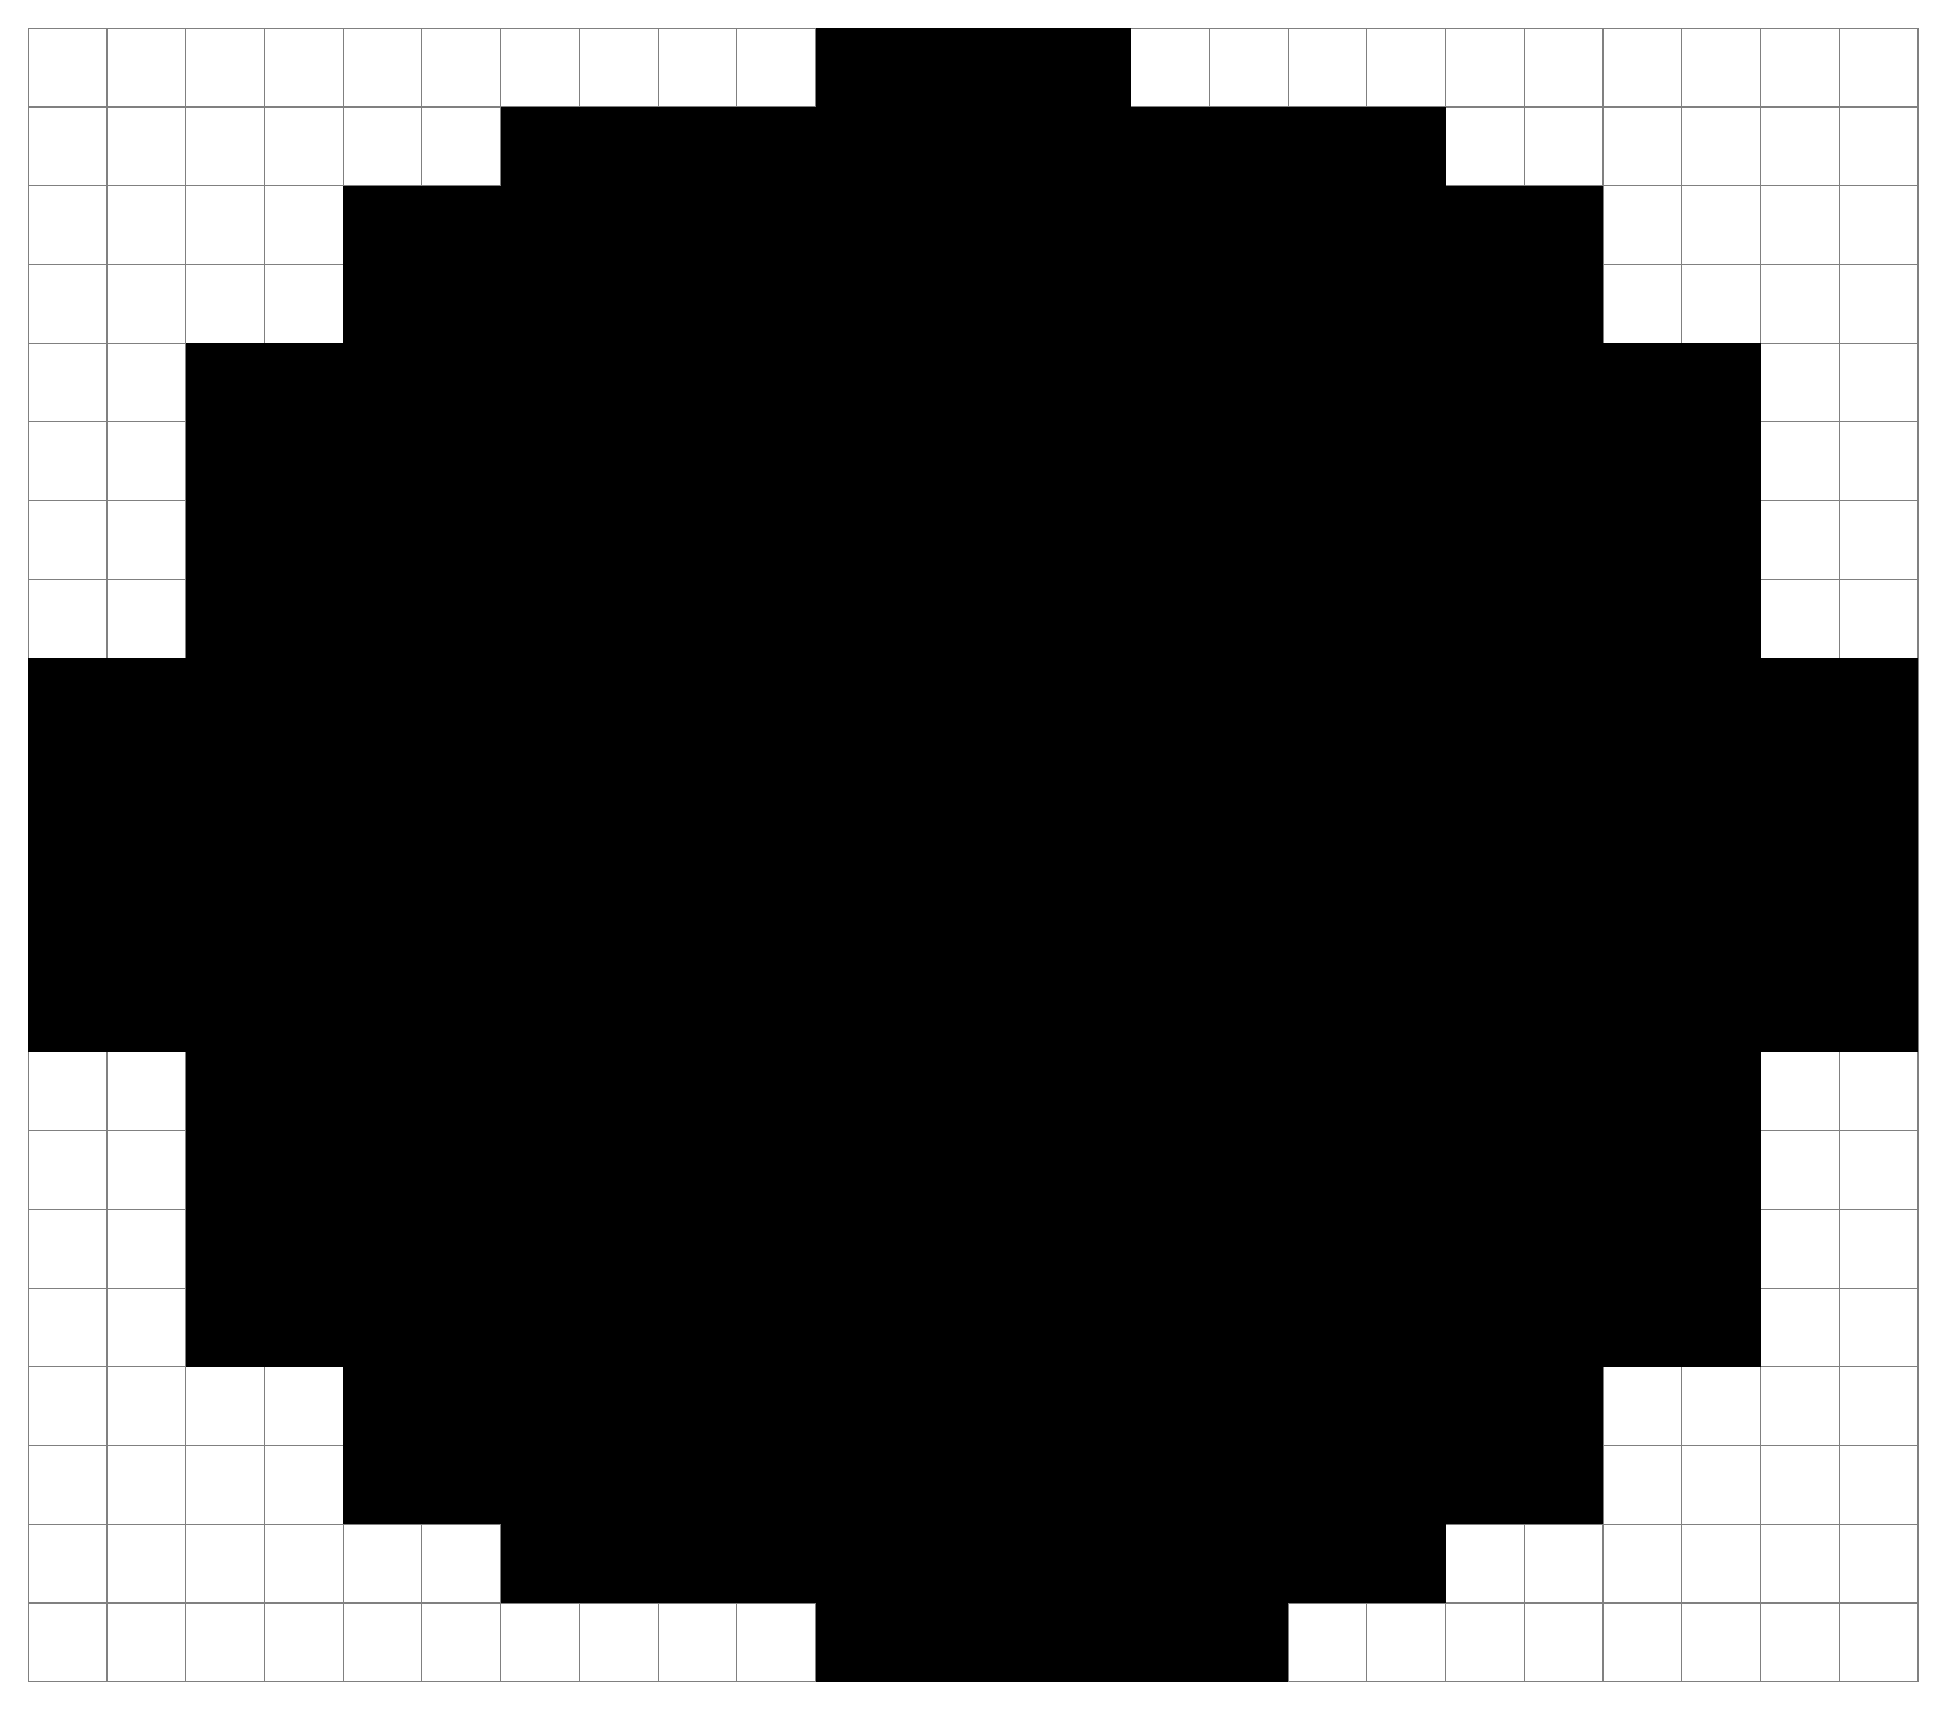
\begin{tikzpicture}

	\draw[step=1.0,gray,thin] (0,0) grid (24,21);
	\fill[\SPRITECOLOR] (10,20) rectangle ++ (1,1);
	\fill[\SPRITECOLOR] (11,20) rectangle ++ (1,1);
	\fill[\SPRITECOLOR] (12,20) rectangle ++ (1,1);
	\fill[\SPRITECOLOR] (13,20) rectangle ++ (1,1);
	\fill[\SPRITECOLOR] (6,19) rectangle ++ (1,1);
	\fill[\SPRITECOLOR] (7,19) rectangle ++ (1,1);
	\fill[\SPRITECOLOR] (8,19) rectangle ++ (1,1);
	\fill[\SPRITECOLOR] (9,19) rectangle ++ (1,1);
	\fill[\SPRITECOLOR] (10,19) rectangle ++ (1,1);
	\fill[\SPRITECOLOR] (11,19) rectangle ++ (1,1);
	\fill[\SPRITECOLOR] (12,19) rectangle ++ (1,1);
	\fill[\SPRITECOLOR] (13,19) rectangle ++ (1,1);
	\fill[\SPRITECOLOR] (14,19) rectangle ++ (1,1);
	\fill[\SPRITECOLOR] (15,19) rectangle ++ (1,1);
	\fill[\SPRITECOLOR] (16,19) rectangle ++ (1,1);
	\fill[\SPRITECOLOR] (17,19) rectangle ++ (1,1);
	\fill[\SPRITECOLOR] (4,18) rectangle ++ (1,1);
	\fill[\SPRITECOLOR] (5,18) rectangle ++ (1,1);
	\fill[\SPRITECOLOR] (6,18) rectangle ++ (1,1);
	\fill[\SPRITECOLOR] (7,18) rectangle ++ (1,1);
	\fill[\SPRITECOLOR] (8,18) rectangle ++ (1,1);
	\fill[\SPRITECOLOR] (9,18) rectangle ++ (1,1);
	\fill[\SPRITECOLOR] (10,18) rectangle ++ (1,1);
	\fill[\SPRITECOLOR] (11,18) rectangle ++ (1,1);
	\fill[\SPRITECOLOR] (12,18) rectangle ++ (1,1);
	\fill[\SPRITECOLOR] (13,18) rectangle ++ (1,1);
	\fill[\SPRITECOLOR] (14,18) rectangle ++ (1,1);
	\fill[\SPRITECOLOR] (15,18) rectangle ++ (1,1);
	\fill[\SPRITECOLOR] (16,18) rectangle ++ (1,1);
	\fill[\SPRITECOLOR] (17,18) rectangle ++ (1,1);
	\fill[\SPRITECOLOR] (18,18) rectangle ++ (1,1);
	\fill[\SPRITECOLOR] (19,18) rectangle ++ (1,1);
	\fill[\SPRITECOLOR] (4,17) rectangle ++ (1,1);
	\fill[\SPRITECOLOR] (5,17) rectangle ++ (1,1);
	\fill[\SPRITECOLOR] (6,17) rectangle ++ (1,1);
	\fill[\SPRITECOLOR] (7,17) rectangle ++ (1,1);
	\fill[\MULTICOLORTWO] (8,17) rectangle ++ (1,1);
	\fill[\MULTICOLORTWO] (9,17) rectangle ++ (1,1);
	\fill[\SPRITECOLOR] (10,17) rectangle ++ (1,1);
	\fill[\SPRITECOLOR] (11,17) rectangle ++ (1,1);
	\fill[\SPRITECOLOR] (12,17) rectangle ++ (1,1);
	\fill[\SPRITECOLOR] (13,17) rectangle ++ (1,1);
	\fill[\SPRITECOLOR] (14,17) rectangle ++ (1,1);
	\fill[\SPRITECOLOR] (15,17) rectangle ++ (1,1);
	\fill[\SPRITECOLOR] (16,17) rectangle ++ (1,1);
	\fill[\SPRITECOLOR] (17,17) rectangle ++ (1,1);
	\fill[\SPRITECOLOR] (18,17) rectangle ++ (1,1);
	\fill[\SPRITECOLOR] (19,17) rectangle ++ (1,1);
	\fill[\SPRITECOLOR] (2,16) rectangle ++ (1,1);
	\fill[\SPRITECOLOR] (3,16) rectangle ++ (1,1);
	\fill[\SPRITECOLOR] (4,16) rectangle ++ (1,1);
	\fill[\SPRITECOLOR] (5,16) rectangle ++ (1,1);
	\fill[\MULTICOLORTWO] (6,16) rectangle ++ (1,1);
	\fill[\MULTICOLORTWO] (7,16) rectangle ++ (1,1);
	\fill[\SPRITECOLOR] (8,16) rectangle ++ (1,1);
	\fill[\SPRITECOLOR] (9,16) rectangle ++ (1,1);
	\fill[\SPRITECOLOR] (10,16) rectangle ++ (1,1);
	\fill[\SPRITECOLOR] (11,16) rectangle ++ (1,1);
	\fill[\SPRITECOLOR] (12,16) rectangle ++ (1,1);
	\fill[\SPRITECOLOR] (13,16) rectangle ++ (1,1);
	\fill[\SPRITECOLOR] (14,16) rectangle ++ (1,1);
	\fill[\SPRITECOLOR] (15,16) rectangle ++ (1,1);
	\fill[\SPRITECOLOR] (16,16) rectangle ++ (1,1);
	\fill[\SPRITECOLOR] (17,16) rectangle ++ (1,1);
	\fill[\SPRITECOLOR] (18,16) rectangle ++ (1,1);
	\fill[\SPRITECOLOR] (19,16) rectangle ++ (1,1);
	\fill[\SPRITECOLOR] (20,16) rectangle ++ (1,1);
	\fill[\SPRITECOLOR] (21,16) rectangle ++ (1,1);
	\fill[\SPRITECOLOR] (2,15) rectangle ++ (1,1);
	\fill[\SPRITECOLOR] (3,15) rectangle ++ (1,1);
	\fill[\SPRITECOLOR] (4,15) rectangle ++ (1,1);
	\fill[\SPRITECOLOR] (5,15) rectangle ++ (1,1);
	\fill[\SPRITECOLOR] (6,15) rectangle ++ (1,1);
	\fill[\SPRITECOLOR] (7,15) rectangle ++ (1,1);
	\fill[\SPRITECOLOR] (8,15) rectangle ++ (1,1);
	\fill[\SPRITECOLOR] (9,15) rectangle ++ (1,1);
	\fill[\SPRITECOLOR] (10,15) rectangle ++ (1,1);
	\fill[\SPRITECOLOR] (11,15) rectangle ++ (1,1);
	\fill[\SPRITECOLOR] (12,15) rectangle ++ (1,1);
	\fill[\SPRITECOLOR] (13,15) rectangle ++ (1,1);
	\fill[\SPRITECOLOR] (14,15) rectangle ++ (1,1);
	\fill[\SPRITECOLOR] (15,15) rectangle ++ (1,1);
	\fill[\SPRITECOLOR] (16,15) rectangle ++ (1,1);
	\fill[\SPRITECOLOR] (17,15) rectangle ++ (1,1);
	\fill[\SPRITECOLOR] (18,15) rectangle ++ (1,1);
	\fill[\SPRITECOLOR] (19,15) rectangle ++ (1,1);
	\fill[\SPRITECOLOR] (20,15) rectangle ++ (1,1);
	\fill[\SPRITECOLOR] (21,15) rectangle ++ (1,1);
	\fill[\SPRITECOLOR] (2,14) rectangle ++ (1,1);
	\fill[\SPRITECOLOR] (3,14) rectangle ++ (1,1);
	\fill[\SPRITECOLOR] (4,14) rectangle ++ (1,1);
	\fill[\SPRITECOLOR] (5,14) rectangle ++ (1,1);
	\fill[\SPRITECOLOR] (6,14) rectangle ++ (1,1);
	\fill[\SPRITECOLOR] (7,14) rectangle ++ (1,1);
	\fill[\SPRITECOLOR] (8,14) rectangle ++ (1,1);
	\fill[\SPRITECOLOR] (9,14) rectangle ++ (1,1);
	\fill[\SPRITECOLOR] (10,14) rectangle ++ (1,1);
	\fill[\SPRITECOLOR] (11,14) rectangle ++ (1,1);
	\fill[\SPRITECOLOR] (12,14) rectangle ++ (1,1);
	\fill[\SPRITECOLOR] (13,14) rectangle ++ (1,1);
	\fill[\SPRITECOLOR] (14,14) rectangle ++ (1,1);
	\fill[\SPRITECOLOR] (15,14) rectangle ++ (1,1);
	\fill[\SPRITECOLOR] (16,14) rectangle ++ (1,1);
	\fill[\SPRITECOLOR] (17,14) rectangle ++ (1,1);
	\fill[\SPRITECOLOR] (18,14) rectangle ++ (1,1);
	\fill[\SPRITECOLOR] (19,14) rectangle ++ (1,1);
	\fill[\SPRITECOLOR] (20,14) rectangle ++ (1,1);
	\fill[\SPRITECOLOR] (21,14) rectangle ++ (1,1);
	\fill[\SPRITECOLOR] (2,13) rectangle ++ (1,1);
	\fill[\SPRITECOLOR] (3,13) rectangle ++ (1,1);
	\fill[\SPRITECOLOR] (4,13) rectangle ++ (1,1);
	\fill[\SPRITECOLOR] (5,13) rectangle ++ (1,1);
	\fill[\SPRITECOLOR] (6,13) rectangle ++ (1,1);
	\fill[\SPRITECOLOR] (7,13) rectangle ++ (1,1);
	\fill[\SPRITECOLOR] (8,13) rectangle ++ (1,1);
	\fill[\SPRITECOLOR] (9,13) rectangle ++ (1,1);
	\fill[\SPRITECOLOR] (10,13) rectangle ++ (1,1);
	\fill[\SPRITECOLOR] (11,13) rectangle ++ (1,1);
	\fill[\SPRITECOLOR] (12,13) rectangle ++ (1,1);
	\fill[\SPRITECOLOR] (13,13) rectangle ++ (1,1);
	\fill[\SPRITECOLOR] (14,13) rectangle ++ (1,1);
	\fill[\SPRITECOLOR] (15,13) rectangle ++ (1,1);
	\fill[\SPRITECOLOR] (16,13) rectangle ++ (1,1);
	\fill[\SPRITECOLOR] (17,13) rectangle ++ (1,1);
	\fill[\SPRITECOLOR] (18,13) rectangle ++ (1,1);
	\fill[\SPRITECOLOR] (19,13) rectangle ++ (1,1);
	\fill[\SPRITECOLOR] (20,13) rectangle ++ (1,1);
	\fill[\SPRITECOLOR] (21,13) rectangle ++ (1,1);
	\fill[\SPRITECOLOR] (0,12) rectangle ++ (1,1);
	\fill[\SPRITECOLOR] (1,12) rectangle ++ (1,1);
	\fill[\SPRITECOLOR] (2,12) rectangle ++ (1,1);
	\fill[\SPRITECOLOR] (3,12) rectangle ++ (1,1);
	\fill[\SPRITECOLOR] (4,12) rectangle ++ (1,1);
	\fill[\SPRITECOLOR] (5,12) rectangle ++ (1,1);
	\fill[\SPRITECOLOR] (6,12) rectangle ++ (1,1);
	\fill[\SPRITECOLOR] (7,12) rectangle ++ (1,1);
	\fill[\MULTICOLORTWO] (8,12) rectangle ++ (1,1);
	\fill[\MULTICOLORTWO] (9,12) rectangle ++ (1,1);
	\fill[\MULTICOLORTWO] (10,12) rectangle ++ (1,1);
	\fill[\MULTICOLORTWO] (11,12) rectangle ++ (1,1);
	\fill[\MULTICOLORTWO] (12,12) rectangle ++ (1,1);
	\fill[\MULTICOLORTWO] (13,12) rectangle ++ (1,1);
	\fill[\MULTICOLORTWO] (14,12) rectangle ++ (1,1);
	\fill[\MULTICOLORTWO] (15,12) rectangle ++ (1,1);
	\fill[\MULTICOLORTWO] (16,12) rectangle ++ (1,1);
	\fill[\MULTICOLORTWO] (17,12) rectangle ++ (1,1);
	\fill[\SPRITECOLOR] (18,12) rectangle ++ (1,1);
	\fill[\SPRITECOLOR] (19,12) rectangle ++ (1,1);
	\fill[\SPRITECOLOR] (20,12) rectangle ++ (1,1);
	\fill[\SPRITECOLOR] (21,12) rectangle ++ (1,1);
	\fill[\SPRITECOLOR] (22,12) rectangle ++ (1,1);
	\fill[\SPRITECOLOR] (23,12) rectangle ++ (1,1);
	\fill[\SPRITECOLOR] (0,11) rectangle ++ (1,1);
	\fill[\SPRITECOLOR] (1,11) rectangle ++ (1,1);
	\fill[\SPRITECOLOR] (2,11) rectangle ++ (1,1);
	\fill[\SPRITECOLOR] (3,11) rectangle ++ (1,1);
	\fill[\MULTICOLORTWO] (4,11) rectangle ++ (1,1);
	\fill[\MULTICOLORTWO] (5,11) rectangle ++ (1,1);
	\fill[\MULTICOLORTWO] (6,11) rectangle ++ (1,1);
	\fill[\MULTICOLORTWO] (7,11) rectangle ++ (1,1);
	\fill[\MULTICOLORTWO] (8,11) rectangle ++ (1,1);
	\fill[\MULTICOLORTWO] (9,11) rectangle ++ (1,1);
	\fill[\MULTICOLORONE] (10,11) rectangle ++ (1,1);
	\fill[\MULTICOLORONE] (11,11) rectangle ++ (1,1);
	\fill[\MULTICOLORONE] (12,11) rectangle ++ (1,1);
	\fill[\MULTICOLORONE] (13,11) rectangle ++ (1,1);
	\fill[\MULTICOLORONE] (14,11) rectangle ++ (1,1);
	\fill[\MULTICOLORONE] (15,11) rectangle ++ (1,1);
	\fill[\MULTICOLORTWO] (16,11) rectangle ++ (1,1);
	\fill[\MULTICOLORTWO] (17,11) rectangle ++ (1,1);
	\fill[\MULTICOLORTWO] (18,11) rectangle ++ (1,1);
	\fill[\MULTICOLORTWO] (19,11) rectangle ++ (1,1);
	\fill[\SPRITECOLOR] (20,11) rectangle ++ (1,1);
	\fill[\SPRITECOLOR] (21,11) rectangle ++ (1,1);
	\fill[\SPRITECOLOR] (22,11) rectangle ++ (1,1);
	\fill[\SPRITECOLOR] (23,11) rectangle ++ (1,1);
	\fill[\SPRITECOLOR] (0,10) rectangle ++ (1,1);
	\fill[\SPRITECOLOR] (1,10) rectangle ++ (1,1);
	\fill[\SPRITECOLOR] (2,10) rectangle ++ (1,1);
	\fill[\SPRITECOLOR] (3,10) rectangle ++ (1,1);
	\fill[\MULTICOLORTWO] (4,10) rectangle ++ (1,1);
	\fill[\MULTICOLORTWO] (5,10) rectangle ++ (1,1);
	\fill[\MULTICOLORTWO] (6,10) rectangle ++ (1,1);
	\fill[\MULTICOLORTWO] (7,10) rectangle ++ (1,1);
	\fill[\MULTICOLORTWO] (8,10) rectangle ++ (1,1);
	\fill[\MULTICOLORTWO] (9,10) rectangle ++ (1,1);
	\fill[\MULTICOLORONE] (10,10) rectangle ++ (1,1);
	\fill[\MULTICOLORONE] (11,10) rectangle ++ (1,1);
	\fill[\MULTICOLORONE] (12,10) rectangle ++ (1,1);
	\fill[\MULTICOLORONE] (13,10) rectangle ++ (1,1);
	\fill[\MULTICOLORONE] (14,10) rectangle ++ (1,1);
	\fill[\MULTICOLORONE] (15,10) rectangle ++ (1,1);
	\fill[\MULTICOLORTWO] (16,10) rectangle ++ (1,1);
	\fill[\MULTICOLORTWO] (17,10) rectangle ++ (1,1);
	\fill[\MULTICOLORTWO] (18,10) rectangle ++ (1,1);
	\fill[\MULTICOLORTWO] (19,10) rectangle ++ (1,1);
	\fill[\MULTICOLORTWO] (20,10) rectangle ++ (1,1);
	\fill[\MULTICOLORTWO] (21,10) rectangle ++ (1,1);
	\fill[\SPRITECOLOR] (22,10) rectangle ++ (1,1);
	\fill[\SPRITECOLOR] (23,10) rectangle ++ (1,1);
	\fill[\SPRITECOLOR] (0,9) rectangle ++ (1,1);
	\fill[\SPRITECOLOR] (1,9) rectangle ++ (1,1);
	\fill[\SPRITECOLOR] (2,9) rectangle ++ (1,1);
	\fill[\SPRITECOLOR] (3,9) rectangle ++ (1,1);
	\fill[\SPRITECOLOR] (4,9) rectangle ++ (1,1);
	\fill[\SPRITECOLOR] (5,9) rectangle ++ (1,1);
	\fill[\MULTICOLORTWO] (6,9) rectangle ++ (1,1);
	\fill[\MULTICOLORTWO] (7,9) rectangle ++ (1,1);
	\fill[\MULTICOLORTWO] (8,9) rectangle ++ (1,1);
	\fill[\MULTICOLORTWO] (9,9) rectangle ++ (1,1);
	\fill[\MULTICOLORONE] (10,9) rectangle ++ (1,1);
	\fill[\MULTICOLORONE] (11,9) rectangle ++ (1,1);
	\fill[\MULTICOLORONE] (12,9) rectangle ++ (1,1);
	\fill[\MULTICOLORONE] (13,9) rectangle ++ (1,1);
	\fill[\MULTICOLORONE] (14,9) rectangle ++ (1,1);
	\fill[\MULTICOLORONE] (15,9) rectangle ++ (1,1);
	\fill[\MULTICOLORTWO] (16,9) rectangle ++ (1,1);
	\fill[\MULTICOLORTWO] (17,9) rectangle ++ (1,1);
	\fill[\MULTICOLORTWO] (18,9) rectangle ++ (1,1);
	\fill[\MULTICOLORTWO] (19,9) rectangle ++ (1,1);
	\fill[\MULTICOLORTWO] (20,9) rectangle ++ (1,1);
	\fill[\MULTICOLORTWO] (21,9) rectangle ++ (1,1);
	\fill[\SPRITECOLOR] (22,9) rectangle ++ (1,1);
	\fill[\SPRITECOLOR] (23,9) rectangle ++ (1,1);
	\fill[\SPRITECOLOR] (0,8) rectangle ++ (1,1);
	\fill[\SPRITECOLOR] (1,8) rectangle ++ (1,1);
	\fill[\SPRITECOLOR] (2,8) rectangle ++ (1,1);
	\fill[\SPRITECOLOR] (3,8) rectangle ++ (1,1);
	\fill[\SPRITECOLOR] (4,8) rectangle ++ (1,1);
	\fill[\SPRITECOLOR] (5,8) rectangle ++ (1,1);
	\fill[\SPRITECOLOR] (6,8) rectangle ++ (1,1);
	\fill[\SPRITECOLOR] (7,8) rectangle ++ (1,1);
	\fill[\MULTICOLORTWO] (8,8) rectangle ++ (1,1);
	\fill[\MULTICOLORTWO] (9,8) rectangle ++ (1,1);
	\fill[\MULTICOLORTWO] (10,8) rectangle ++ (1,1);
	\fill[\MULTICOLORTWO] (11,8) rectangle ++ (1,1);
	\fill[\MULTICOLORTWO] (12,8) rectangle ++ (1,1);
	\fill[\MULTICOLORTWO] (13,8) rectangle ++ (1,1);
	\fill[\MULTICOLORTWO] (14,8) rectangle ++ (1,1);
	\fill[\MULTICOLORTWO] (15,8) rectangle ++ (1,1);
	\fill[\MULTICOLORTWO] (16,8) rectangle ++ (1,1);
	\fill[\MULTICOLORTWO] (17,8) rectangle ++ (1,1);
	\fill[\SPRITECOLOR] (18,8) rectangle ++ (1,1);
	\fill[\SPRITECOLOR] (19,8) rectangle ++ (1,1);
	\fill[\SPRITECOLOR] (20,8) rectangle ++ (1,1);
	\fill[\SPRITECOLOR] (21,8) rectangle ++ (1,1);
	\fill[\SPRITECOLOR] (22,8) rectangle ++ (1,1);
	\fill[\SPRITECOLOR] (23,8) rectangle ++ (1,1);
	\fill[\SPRITECOLOR] (2,7) rectangle ++ (1,1);
	\fill[\SPRITECOLOR] (3,7) rectangle ++ (1,1);
	\fill[\SPRITECOLOR] (4,7) rectangle ++ (1,1);
	\fill[\SPRITECOLOR] (5,7) rectangle ++ (1,1);
	\fill[\SPRITECOLOR] (6,7) rectangle ++ (1,1);
	\fill[\SPRITECOLOR] (7,7) rectangle ++ (1,1);
	\fill[\SPRITECOLOR] (8,7) rectangle ++ (1,1);
	\fill[\SPRITECOLOR] (9,7) rectangle ++ (1,1);
	\fill[\SPRITECOLOR] (10,7) rectangle ++ (1,1);
	\fill[\SPRITECOLOR] (11,7) rectangle ++ (1,1);
	\fill[\SPRITECOLOR] (12,7) rectangle ++ (1,1);
	\fill[\SPRITECOLOR] (13,7) rectangle ++ (1,1);
	\fill[\SPRITECOLOR] (14,7) rectangle ++ (1,1);
	\fill[\SPRITECOLOR] (15,7) rectangle ++ (1,1);
	\fill[\SPRITECOLOR] (16,7) rectangle ++ (1,1);
	\fill[\SPRITECOLOR] (17,7) rectangle ++ (1,1);
	\fill[\SPRITECOLOR] (18,7) rectangle ++ (1,1);
	\fill[\SPRITECOLOR] (19,7) rectangle ++ (1,1);
	\fill[\SPRITECOLOR] (20,7) rectangle ++ (1,1);
	\fill[\SPRITECOLOR] (21,7) rectangle ++ (1,1);
	\fill[\SPRITECOLOR] (2,6) rectangle ++ (1,1);
	\fill[\SPRITECOLOR] (3,6) rectangle ++ (1,1);
	\fill[\SPRITECOLOR] (4,6) rectangle ++ (1,1);
	\fill[\SPRITECOLOR] (5,6) rectangle ++ (1,1);
	\fill[\SPRITECOLOR] (6,6) rectangle ++ (1,1);
	\fill[\SPRITECOLOR] (7,6) rectangle ++ (1,1);
	\fill[\SPRITECOLOR] (8,6) rectangle ++ (1,1);
	\fill[\SPRITECOLOR] (9,6) rectangle ++ (1,1);
	\fill[\SPRITECOLOR] (10,6) rectangle ++ (1,1);
	\fill[\SPRITECOLOR] (11,6) rectangle ++ (1,1);
	\fill[\SPRITECOLOR] (12,6) rectangle ++ (1,1);
	\fill[\SPRITECOLOR] (13,6) rectangle ++ (1,1);
	\fill[\SPRITECOLOR] (14,6) rectangle ++ (1,1);
	\fill[\SPRITECOLOR] (15,6) rectangle ++ (1,1);
	\fill[\SPRITECOLOR] (16,6) rectangle ++ (1,1);
	\fill[\SPRITECOLOR] (17,6) rectangle ++ (1,1);
	\fill[\SPRITECOLOR] (18,6) rectangle ++ (1,1);
	\fill[\SPRITECOLOR] (19,6) rectangle ++ (1,1);
	\fill[\SPRITECOLOR] (20,6) rectangle ++ (1,1);
	\fill[\SPRITECOLOR] (21,6) rectangle ++ (1,1);
	\fill[\SPRITECOLOR] (2,5) rectangle ++ (1,1);
	\fill[\SPRITECOLOR] (3,5) rectangle ++ (1,1);
	\fill[\SPRITECOLOR] (4,5) rectangle ++ (1,1);
	\fill[\SPRITECOLOR] (5,5) rectangle ++ (1,1);
	\fill[\SPRITECOLOR] (6,5) rectangle ++ (1,1);
	\fill[\SPRITECOLOR] (7,5) rectangle ++ (1,1);
	\fill[\SPRITECOLOR] (8,5) rectangle ++ (1,1);
	\fill[\SPRITECOLOR] (9,5) rectangle ++ (1,1);
	\fill[\SPRITECOLOR] (10,5) rectangle ++ (1,1);
	\fill[\SPRITECOLOR] (11,5) rectangle ++ (1,1);
	\fill[\SPRITECOLOR] (12,5) rectangle ++ (1,1);
	\fill[\SPRITECOLOR] (13,5) rectangle ++ (1,1);
	\fill[\SPRITECOLOR] (14,5) rectangle ++ (1,1);
	\fill[\SPRITECOLOR] (15,5) rectangle ++ (1,1);
	\fill[\SPRITECOLOR] (16,5) rectangle ++ (1,1);
	\fill[\SPRITECOLOR] (17,5) rectangle ++ (1,1);
	\fill[\SPRITECOLOR] (18,5) rectangle ++ (1,1);
	\fill[\SPRITECOLOR] (19,5) rectangle ++ (1,1);
	\fill[\SPRITECOLOR] (20,5) rectangle ++ (1,1);
	\fill[\SPRITECOLOR] (21,5) rectangle ++ (1,1);
	\fill[\SPRITECOLOR] (2,4) rectangle ++ (1,1);
	\fill[\SPRITECOLOR] (3,4) rectangle ++ (1,1);
	\fill[\SPRITECOLOR] (4,4) rectangle ++ (1,1);
	\fill[\SPRITECOLOR] (5,4) rectangle ++ (1,1);
	\fill[\SPRITECOLOR] (6,4) rectangle ++ (1,1);
	\fill[\SPRITECOLOR] (7,4) rectangle ++ (1,1);
	\fill[\SPRITECOLOR] (8,4) rectangle ++ (1,1);
	\fill[\SPRITECOLOR] (9,4) rectangle ++ (1,1);
	\fill[\SPRITECOLOR] (10,4) rectangle ++ (1,1);
	\fill[\SPRITECOLOR] (11,4) rectangle ++ (1,1);
	\fill[\SPRITECOLOR] (12,4) rectangle ++ (1,1);
	\fill[\SPRITECOLOR] (13,4) rectangle ++ (1,1);
	\fill[\SPRITECOLOR] (14,4) rectangle ++ (1,1);
	\fill[\SPRITECOLOR] (15,4) rectangle ++ (1,1);
	\fill[\SPRITECOLOR] (16,4) rectangle ++ (1,1);
	\fill[\SPRITECOLOR] (17,4) rectangle ++ (1,1);
	\fill[\SPRITECOLOR] (18,4) rectangle ++ (1,1);
	\fill[\SPRITECOLOR] (19,4) rectangle ++ (1,1);
	\fill[\SPRITECOLOR] (20,4) rectangle ++ (1,1);
	\fill[\SPRITECOLOR] (21,4) rectangle ++ (1,1);
	\fill[\SPRITECOLOR] (4,3) rectangle ++ (1,1);
	\fill[\SPRITECOLOR] (5,3) rectangle ++ (1,1);
	\fill[\SPRITECOLOR] (6,3) rectangle ++ (1,1);
	\fill[\SPRITECOLOR] (7,3) rectangle ++ (1,1);
	\fill[\SPRITECOLOR] (8,3) rectangle ++ (1,1);
	\fill[\SPRITECOLOR] (9,3) rectangle ++ (1,1);
	\fill[\SPRITECOLOR] (10,3) rectangle ++ (1,1);
	\fill[\SPRITECOLOR] (11,3) rectangle ++ (1,1);
	\fill[\SPRITECOLOR] (12,3) rectangle ++ (1,1);
	\fill[\SPRITECOLOR] (13,3) rectangle ++ (1,1);
	\fill[\SPRITECOLOR] (14,3) rectangle ++ (1,1);
	\fill[\SPRITECOLOR] (15,3) rectangle ++ (1,1);
	\fill[\SPRITECOLOR] (16,3) rectangle ++ (1,1);
	\fill[\SPRITECOLOR] (17,3) rectangle ++ (1,1);
	\fill[\SPRITECOLOR] (18,3) rectangle ++ (1,1);
	\fill[\SPRITECOLOR] (19,3) rectangle ++ (1,1);
	\fill[\SPRITECOLOR] (4,2) rectangle ++ (1,1);
	\fill[\SPRITECOLOR] (5,2) rectangle ++ (1,1);
	\fill[\SPRITECOLOR] (6,2) rectangle ++ (1,1);
	\fill[\SPRITECOLOR] (7,2) rectangle ++ (1,1);
	\fill[\SPRITECOLOR] (8,2) rectangle ++ (1,1);
	\fill[\SPRITECOLOR] (9,2) rectangle ++ (1,1);
	\fill[\SPRITECOLOR] (10,2) rectangle ++ (1,1);
	\fill[\SPRITECOLOR] (11,2) rectangle ++ (1,1);
	\fill[\SPRITECOLOR] (12,2) rectangle ++ (1,1);
	\fill[\SPRITECOLOR] (13,2) rectangle ++ (1,1);
	\fill[\SPRITECOLOR] (14,2) rectangle ++ (1,1);
	\fill[\SPRITECOLOR] (15,2) rectangle ++ (1,1);
	\fill[\SPRITECOLOR] (16,2) rectangle ++ (1,1);
	\fill[\SPRITECOLOR] (17,2) rectangle ++ (1,1);
	\fill[\SPRITECOLOR] (18,2) rectangle ++ (1,1);
	\fill[\SPRITECOLOR] (19,2) rectangle ++ (1,1);
	\fill[\SPRITECOLOR] (6,1) rectangle ++ (1,1);
	\fill[\SPRITECOLOR] (7,1) rectangle ++ (1,1);
	\fill[\SPRITECOLOR] (8,1) rectangle ++ (1,1);
	\fill[\SPRITECOLOR] (9,1) rectangle ++ (1,1);
	\fill[\SPRITECOLOR] (10,1) rectangle ++ (1,1);
	\fill[\SPRITECOLOR] (11,1) rectangle ++ (1,1);
	\fill[\SPRITECOLOR] (12,1) rectangle ++ (1,1);
	\fill[\SPRITECOLOR] (13,1) rectangle ++ (1,1);
	\fill[\SPRITECOLOR] (14,1) rectangle ++ (1,1);
	\fill[\SPRITECOLOR] (15,1) rectangle ++ (1,1);
	\fill[\SPRITECOLOR] (16,1) rectangle ++ (1,1);
	\fill[\SPRITECOLOR] (17,1) rectangle ++ (1,1);
	\fill[\SPRITECOLOR] (10,0) rectangle ++ (1,1);
	\fill[\SPRITECOLOR] (11,0) rectangle ++ (1,1);
	\fill[\SPRITECOLOR] (12,0) rectangle ++ (1,1);
	\fill[\SPRITECOLOR] (13,0) rectangle ++ (1,1);
	\fill[\SPRITECOLOR] (14,0) rectangle ++ (1,1);
	\fill[\SPRITECOLOR] (15,0) rectangle ++ (1,1);

      \end{tikzpicture}
    \end{adjustbox}
  }\caption{BONUS\_IBALL4}
\end{figure}

	\end{subfigure}
} \\ 
        \addlinespace
        \bottomrule
      \end{tabular}
    \end{adjustbox}
  }\caption{OK this is better.}
\end{figure}


